
%   Template - Institute of Control Systems, TUHH

%#############################################################################
%     R E A D      M E     F I R S T  !
%#############################################################################
% For setting up a latex enviroment, please follow: https://www.latexbuch.de/latex-windows-installieren/
% In Texmaker you can setup fast compile with these arguments: lualatex -interaction=nonstopmode %.tex|biber %|lualatex -interaction=nonstopmode %.tex|"C:/Program Files/Adobe/Reader 11.0/Reader/AcroRd32.exe" %.pdf
% Possible compilation processes:
% Luatex -> biber -> Luatex 
% For texstudio: lualatex.exe -synctex=1 -interaction=nonstopmode --enable-write18 -interaction=nonstopmode %.tex or 
% pdflatex.exe -synctex=1 -interaction=nonstopmode -shell-escape --enable-write18 -interaction=nonstopmode %.tex
% enables the compiler to use tikz externalize as well
% Toolchain is than: PDFLatex: txs:///pdflatex | txs:///biber | txs:///pdflatex | txs:///view-pdf-internal --embedded
%					  LuaLatex: txs:///lualatex | txs:///biber | txs:///lualatex | txs:///view-pdf-internal --embedded
% VS-Code + LatexWorkshop: Config-File in header/VS_Settings.pdf
%#############################################################################
% CITATION:
% use \cite{bibkey} to cite the desired literature
%#############################################################################

%%################ Language settings #########################################
% Language settings:
% change to false for German language
\def\isenglish{true}

% draft setting:
\def\isDraft{false}

 %%################ Document settings #########################################
\def\curdir{}
\documentclass[compress]{beamer}

\mode<presentation>
{
  \usetheme{RT}
  \setbeamercovered{transparent}
  \usecolortheme{RT}
}

\setbeamertemplate{navigation symbols}{}
\setbeamertemplate{footline}[frame number]{}


\usepackage{ifthen}
\ifthenelse{\equal{\isenglish}{true}}{
	%%% English
	\usepackage[german, ngerman, english]{babel}
	\selectlanguage{english}
}{
	%%% German
	\usepackage[english, german, ngerman]{babel}
	\selectlanguage{german}
}

\usepackage{lmodern}
\usepackage{csquotes}
\usepackage{microtype}
\ifluatex
	\usepackage{fontspec}
\else
	\usepackage[utf8]{inputenc}
\fi

%% Allow usage of the part command to create different navigations parts 
\usepackage{xpatch}
\makeatletter
\xpatchcmd{\beamer@part}{\Hy@writebookmark{\the\c@section}{#1}{Outline\the\c@part}{1}{toc}}{}{}{}
\makeatother

\usepackage{appendixnumberbeamer}

\makeatletter
\AtBeginPart{%
  \beamer@tocsectionnumber=0\relax
  \setcounter{section}{0}
%   \frame{\partpage}%
}
\makeatother


 %%######## GRAPHICS Options
\graphicspath{{figures/}}				% Define the path to the figures

\usepackage{ifpdf}

 % Other figures (e.g., MATLAB  EPS or PDF figures)
\newcommand{\afig}[2]{\includegraphics[scale=#1]{#2}}

 % figures defined in TeX files
\newcommand{\tfig}[2]{\scalebox{#1}{\input{"#2.tex"}}}

\usepackage{multimedia}
\usepackage{tikz}

\usetikzlibrary{%
  arrows,%
  arrows.meta,
  shapes.misc,% wg. rounded rectangle
  shapes.arrows,
  shapes.misc,
  calc,
  plotmarks,
  chains,%
  matrix,%
  positioning,% wg. " of "
  scopes,%
  decorations.pathmorphing,% /pgf/decoration/random steps | erste Graphik
  decorations.markings,
  shadows%
}
\usetikzlibrary{external}
\tikzexternalize[prefix=figures/0externalize/] % activate!
\usepackage{pgfplots}
\pgfplotsset{compat=newest}

\newlength{\figw}
\setlength{\figw}{0.8\textwidth}
\newlength{\figh}
\setlength{\figh}{0.4\textwidth}

\newcommand{\tikzfig}[2]{
  \tikzsetnextfilename{#2}%
  \scalebox{#1}{
    \input{"figures/#2.tex"}}
}

 %%######## Logos only on Title page
% \titlegraphic{\vspace{0.1cm}\includegraphics[height=0.8cm]{admin/} \hfill \includegraphics[height=0.7cm]{Logo_ICS_4c}}

\titlegraphic{
	\vspace{1cm}
	\begin{minipage}{0.5\textwidth}
		\begin{flushleft} \large
			\ifthenelse{\equal{\isenglish}{true}}
			{\includegraphics[height=0.8cm]{admin/Logo_TUHH_rgb_en}}
			{\includegraphics[height=0.8cm]{admin/Logo_TUHH_rgb_de}}
		\end{flushleft}
	\end{minipage}
	\hfill
	\begin{minipage}{0.4\textwidth}
		\begin{flushright} \large
			\includegraphics[height=0.8cm]{admin/Logo_ICS_4c} % Supervisor's Name
		\end{flushright}
	\end{minipage}\\[0.4cm]
}

 %%######## Other FUNCTIONS

 % Some color definitions
\setbeamercolor{greenhead}{fg=white,bg=green!80!black}%
\setbeamercolor{greenbody}{fg=black,bg=green!50!white}%

\setbeamercolor{redhead}{fg=white,bg=red!80!black}%
\setbeamercolor{redbody}{fg=black,bg=red!50!white}%


\usepackage{epstopdf}

\usepackage[style=ieee,backend=biber]{biblatex} %% bibliography
\addbibresource{ics.bib}

 %%############################################################################
 %%################## Thesis Data #############################################
 % include the file thesis_data_lastname_firstname.tex here 
 % You will receive this file from your supervisor




 %%#######################################################
 %%################## Thesis Data ######################

% Student Entry No.               1

\def\titlenameEN{Comparison of data-driven control algorithms using Koopman operator and LPV
techniques for evaluating the tracking performance of an Arm-Driven Inverted Pendulum}

\def\titlenameDE{Vergleich von datengetriebenen Regelungsalgorithmen basierend auf dem Koopman Operator und LPV-Techniken zur Evaluation der Tracking-Performance eines armgetriebenen invertierten Pendels
}

\def\authorfirstname{Yashasvi Sai}
\def\authorfamilyname{Sukhavasi}

% f: female
% m: male 
\def\gender{m}

\def\studentid{21757720}

\def\studycourse{IMPMEC}

% p: project work
% b: bachelor thesis
% m: master's thesis
\def\thesistype{m}

\def\thesisnumber{\MakeUppercase{\thesistype} --- 7 --- 2020}

\def\supervisornameI {Patrick Göttsch, M.Sc.}


\def\supervisornameII {}


\def\examinernameI {Prof. Dr. Herbert Werner}


\def\examinernameII {Prof. Dr. Tobias Knopp}

% If written externally, like in a Company or at another university, note this university here
% A supervisor of the company can be put as supervisor
\def\ExternalCompany {}

% Shows if the thesis is under NDA, only displayed when ExternalCompany is set
% false: no NDA
% true: NDA
\def\HasNDA {false}
% Set date until the NDA is agreed, normally duedate + 3 years
\def\NDAdueDate {}


\def\startdate{16.06.2020}

\def\duedate{20.01.2021}

\def\todaydate{26.06.2020}


 % Project description
\def\projectdescription{
The Koopman operator theory \cite{Koopman1931}, is an increasingly popular formalism of dynamical systems theory that enables analysis, prediction and control of nonlinear dynamics from measurement data. Such data-driven techniques allow for devising linear control strategies for highly nonlinear dynamical systems for which first principle models are not available or are impractical to be constructed.\par
The motivation for this Master's thesis is derived from the desire to generate dynamical models of an ADIP through measured data. In particular it is of interest to synthesize linear model-based controllers using these data-driven models in simulation and experimentally compare the performance of data-driven controllers with LPV contrrollers based on first principles in tracking a reference trajectory.
}

 % Project tasks
\def\tasks{
\begin{packedenumerate}
	\item Literature review of state-of-the-art architecture for data-driven control systems
	\item Develop a data-driven approach using Koopman operator theory for constructing a linear representation of the ADIP plant for the purpose of swing-up and stabilizing control
    	\item Synthesize a quasi-LPV controller governing the swing-up dynamics and a stabilizing Linear Quadratic Regulator and a stabilizing quasi-LPV controller for the aforementioned data-driven model
    	\item Simulate and compare the performance of the derived controllers in tracking a reference trajectory
    	\item Experimentally validate the simulation results
    	\item Optional: Extend the above framework to synthesizing a stabilizing data-driven quasi-LPV Predictive Controller using Koopman operator techniques(KqLMPC) and compare it with the existing results on the performance of qLMPC control strategy applied on the model obtained from first principles, \cite{qLMPC}. 

\end{packedenumerate}
}

% #########todo
\setlength {\marginparwidth }{2cm}
\usepackage[colorinlistoftodos]{todonotes}
 %%##############################  CONTENTS ###################################
\begin{document}

 %% Title page
\thispagestyle{empty}
\begin{titlepage}

 %%################ general settings ###################
\definecolor{darkBlue}{rgb}{0, 0.255, 0.471} 
\newcommand{\HRule}{\textcolor{darkBlue}{\rule{\textwidth}{0.4mm}}} % Defines a new command for the horizontal lines, change thickness here
\center % Center everything on the page

% thesis type
\ifthenelse{\equal{\isenglish}{true}}{
	\ifthenelse{\equal{\thesistype}{m}}{
		\def\thesisname{Master's thesis}}
	{\ifthenelse{\equal{\thesistype}{b}}{
		\def\thesisname{Bachelor thesis}}
	{\ifthenelse{\equal{\thesistype}{p}}{
		\def\thesisname{Project work}}{
		\def\thesisname{\thesistype}
	}}}
}
{
	\ifthenelse{\equal{\thesistype}{m}}{
		\def\thesisname{Masterarbeit}}
	{\ifthenelse{\equal{\thesistype}{b}}{
		\def\thesisname{Bachelorarbeit}}
	{\ifthenelse{\equal{\thesistype}{p}}{
		\def\thesisname{Projektarbeit}}{
		\def\thesisname{\thesistype}
	}}}
}

 %%################ logo section ###################
\HRule \\[0.4cm]
\begin{minipage}{0.5\textwidth}
\begin{flushleft} \large
	\ifthenelse{\equal{\isenglish}{true}}
	{\includegraphics[height=2cm]{admin/Logo_TUHH_en}}
	{
\includegraphics[height=2cm]{admin/Logo_TUHH_de}}
\end{flushleft}
\end{minipage}
\hfill
\begin{minipage}{0.4\textwidth}
\begin{flushright} \large
\includegraphics[height=2cm]{admin/Logo_ICS_4c} % Supervisor's Name
\end{flushright}
\end{minipage}\\[0.4cm]

\HRule \\[3cm]
 {\large \textsc{\thesisname}}\\[1cm]
{\fontsize{32}{32}\selectfont
\ifthenelse{\equal{\isenglish}{true}}{\titlenameEN}{\titlenameDE}\par
}

\vfill

 %%################ author and date section ###################

\begin{minipage}[b]{0.6\textwidth}
\begin{flushleft} \large
\ifthenelse{\equal{\isenglish}{true}}{\emph{Author:}}{\emph{Autor:}}\\
\authorfirstname\, \authorfamilyname \\[1cm] % Your name
%\ifthenelse{\equal{\isenglish}{true}}{\emph{Supervisors:}}{\emph{Betreuer:}} \\
%\supervisorname
%\ifthenelse{\equal{\isenglish}{true}}{\emph{Examiners:}}{\emph{Gutachter:}} \\
%\examinername

%%################ Supervison section ###################
\begin{tabbing}
\textbf{\ifthenelse{\equal{\isenglish}{true}}{Supervisor:}{Betreuer:\hspace{0.4cm}}} \= \phantom{1.} \= \supervisornameI \\ \> \phantom{2.} \> \supervisornameII \\
\textbf{\ifthenelse{\equal{\isenglish}{true}}{Examiner:}{Prüfer:}} \> \ifthenelse{\equal{\examinernameII}{}}{}{1.}  \> \examinernameI \\
\ifthenelse{\equal{\examinernameII}{}}{}{\> 2. \> \examinernameII}
\end{tabbing}

\end{flushleft}
\end{minipage}
\hfill
\begin{minipage}{0.3\textwidth}
\begin{flushright}
{\large \today} % Date, change the \today to a set date if you want to be precise
\end{flushright}
\end{minipage}

\HRule 
\end{titlepage}

\newpage
\thispagestyle{empty}
\mbox{}
\newpage


 %% Project description
 %%################ settings ###################
\thispagestyle{empty}
\definecolor{darkBlue}{rgb}{0, 0.255, 0.471} 
\newcommand{\HRule}{\textcolor{darkBlue}{\rule{\textwidth}{0.4mm}}} 

\ifthenelse{\equal{\isenglish}{true}}
{\def\bibnamep{References}}%
{\def\bibnamep{Literatur}}%

% thesis type
\ifthenelse{\equal{\isenglish}{true}}{
	\ifthenelse{\equal{\thesistype}{m}}{
		\def\thesisname{Master's thesis}}
	{\ifthenelse{\equal{\thesistype}{b}}{
		\def\thesisname{Bachelor thesis}}
	{\ifthenelse{\equal{\thesistype}{p}}{
		\def\thesisname{Project Work}}{
		\def\thesisname{\thesistype}
	}}}
}
{
	\ifthenelse{\equal{\thesistype}{m}}{
		\def\thesisname{Masterarbeit}}
	{\ifthenelse{\equal{\thesistype}{b}}{
		\def\thesisname{Bachelorarbeit}}
	{\ifthenelse{\equal{\thesistype}{p}}{
		\def\thesisname{Projektarbeit}}{
		\def\thesisname{\thesistype}
	}}}
}

%%################ PDF Info Section #################
\ifthenelse{\equal{\thesistype}{m}}{
	\def\thesisnamePDF{Master's thesis}}
	{\ifthenelse{\equal{\thesistype}{b}}{
		\def\thesisnamePDF{Bachelor thesis}}
		{\ifthenelse{\equal{\thesistype}{p}}{
			\def\thesisnamePDF{Project Work}}{
			\def\thesisnamePDF{\thesistype}
}}}

\hypersetup{
	pdfauthor		={\authorfamilyname, \authorfirstname},
	pdftitle		={\titlenameEN},
	pdfsubject		={Project Description for \thesisnamePDF},
	pdfproducer		={LaTeX},
	pdfcreator		={LuLaTeX}
}

%%################ logo section ###################
\ifthenelse{\equal{\isDraft}{true}}{
	\newwatermark[firstpage,color=red!30,angle=22,scale=2,xpos=20,ypos=90]{DRAFT}
}{ }
\begin{flushright}
\includegraphics[height=1.7cm]{admin/Logo_ICS_4c} % Supervisor's Name
\end{flushright}
\vspace{-0.7cm}

 %%################ Data section ###################
\HRule\\[0.4cm]
\begin{minipage}[b]{0.38\textwidth}
\begin{flushleft} 
\textbf{\thesisname}
\end{flushleft}
\end{minipage}
\hfill
\begin{minipage}{0.3\textwidth}
\begin{center}
\textbf{\thesisnumber}
\end{center}
\end{minipage}
\hfill
\begin{minipage}{0.3\textwidth}
\begin{flushright}

\end{flushright}
\end{minipage}\\
\begin{minipage}[b]{0.38\textwidth}
\begin{flushleft} 
\ifthenelse{\equal{\isenglish}{true}}{for \ifthenelse{\equal{\gender}{m}}{Mr.}{Ms.}}{für \ifthenelse{\equal{\gender}{m}}{Herrn}{Frau}\textbf{}} \authorfirstname\, \authorfamilyname
\end{flushleft}
\end{minipage}
\hfill
\begin{minipage}{0.3\textwidth}
\begin{center}
\ifthenelse{\equal{\isenglish}{true}}{Student ID:}{Matr.-Nr.:} \studentid
\end{center}
\end{minipage}
\hfill
\begin{minipage}{0.3\textwidth}
\begin{flushright}
\ifthenelse{\equal{\isenglish}{true}}{Study Course:}{Studiengang:} \studycourse
\end{flushright}
\end{minipage}
\HRule
\begin{refsection}
	 %%################ Task section ###################
	\vspace{1em}
	\newline
	\textbf{\ifthenelse{\equal{\isenglish}{true}}{Title:\\\titlenameEN}{Titel:\\\titlenameDE}}
	\ifthenelse{\equal{\isDraft}{true}}{
		\newline
		\ifthenelse{\equal{\isenglish}{false}}{Title: \titlenameEN}{Titel: \titlenameDE}
	}{}
	\paragraph*{\ifthenelse{\equal{\isenglish}{true}}{Project Description:\\}{Beschreibung:\\}}\projectdescription
	\paragraph*{\ifthenelse{\equal{\isenglish}{true}}{Tasks:\\}{Aufgaben:\\}\vspace{-0.8cm}}\tasks
	
	\newpage
	%%################ Literatur section ###################
	\begingroup
		\paragraph*{\bibnamep:\\\vspace{-0.5cm}}
		\renewcommand{\section}[2]{}%
		{\fontsize{10}{11}\selectfont \printbibliography}
	\endgroup
\end{refsection}

 %%################ Supervison section ###################
\begin{tabbing}
	\textbf{\ifthenelse{\equal{\isenglish}{true}}{Supervisor:}{Betreuer:\hspace{0.3cm}}} \= \phantom{1.} \= \supervisornameI \ifthenelse{\equal{\supervisornameII}{}}{\\}{\\ \> \phantom{2.} \> \supervisornameII \\}
	\textbf{\ifthenelse{\equal{\isenglish}{true}}{Examiner:}{Prüfer:}} \> 1. \> \examinernameI \ifthenelse{\equal{\examinernameII}{}}{\\}{\\ \> 2. \> \examinernameII \\}
	% External Company
	\ifthenelse{\equal{\ExternalCompany}{}}
	{}
	{
		\; \> \; \> \;\\
		\textbf{\ifthenelse{\equal{\isenglish}{true}}
		{External:}
		{Extern:}
		} \> \; \> \ExternalCompany
		\ifthenelse{\equal{\HasNDA}{true}}
		{\ifthenelse{\equal{\isenglish}{true}}{\;(NDA until \NDAdueDate)}{\;(NDA bis \NDAdueDate)}}
		{}
		\\
	}
\end{tabbing}
\vspace{-0.5cm}
%%################ Title ##########################
\ifthenelse{\equal{\isenglish}{false}}{\textbf{English title:} \titlenameEN}{{\textbf{Deutscher Titel:}} \titlenameDE}
%%################ Date section ###################
% \vspace{-0.5cm}
\begin{tabbing}
	\textbf{\ifthenelse{\equal{\isenglish}{true}}{Start Date:}{Ausgabe der Arbeit:}} \= \phantom{1.} \= \startdate \\
	\textbf{\ifthenelse{\equal{\isenglish}{true}}{Due Date:}{Abgabe der Arbeit:}} \> \phantom{1.} \> \duedate
\end{tabbing}

 %%################ Signature section ###################
\vspace{2cm}
\todaydate, Prof.\ Dr.\ H.\ Werner

 %% Declaration
\newpage
\thispagestyle{empty}
\vspace{3cm}

\ifthenelse{\equal{\isenglish}{true}}{
Hereby I declare that I produced the present work myself only with the help of the indicated aids and sources.}
{
Hiermit erkl\"are ich, die vorliegende Arbeit selbstst\"andig durchgef\"uhrt und keine weiteren Hilfsmittel und Quellen als die angegebenen genutzt zu haben.
}
\vspace{3cm}

Hamburg, \today  \hfill  \authorfirstname\, \authorfamilyname
\cleardoublepage

 %% Abstract
\thispagestyle{empty}
\ifthenelse{\equal{\isenglish}{true}}%
{
\section*{Abstract}
This work investigates the Koopman operator framework's implementation to approximate linear predictors for the Arm-Driven Inverted Pendulum, a nonlinear controlled dynamical system. The Koopman approach promises to apply the tools developed for linear dynamical systems to the dynamical systems defined by the Koopman operator; thus obtaining a linear approximation of a nonlinear system without directly linearizing around a fixed point. This is done by lifting or embedding the underlying nonlinear dynamics into a higher dimensional space where the Koopman operator's evolution is approximately linear. Although linear, the Koopman operator is infinite-dimensional, which renders it unsuitable for application purposes and therefore, a finite-dimensional approximation is computed by applying the Extended Dynamic Mode Decomposition. Such models' tracking performance is evaluated against a model obtained from first-principles linearized around a fixed point. It is seen that the Koopman model exhibits performance superior to a locally linearized model. Importantly, the approach to compute such a model is completely data-driven and extremely simple. It involves only a nonlinear transformation of the measured data (also called \textit{lifting} the dimension of the data) and a linear least-squares problem in the higher dimensional lifted space that can be readily solved even for large data sets. This approximated linear Koopman model can be readily used to synthesize controllers for the underlying nonlinear dynamical system using linear control design methodologies. This work also compares the performance of non-predictive controllers obtained in this way against that of predictive controllers. Predictive controllers such as the Model Predictive Controller offers numerous advantages over non-predictive controllers such as the Linear Quadratic Regulator, more so in the case of data-driven control.
}
{
\section*{Zusammenfassung}
Hier sollte eine kurze Zusammenfassung Ihrer Arbeit stehen, die einem Leser eine Übersicht über die Aufgabenstellung und die erzielten Ergebnisse gibt.
Dieser Text wird auch in der öffenlichen Ankündigung zu Ihrem Abschlussvortrag erscheinen, also geben Sie sich Mühe, es kurz, verständlich und auf die wesentlichen Punkte beschränkt zu halten.

Für den folgenden Text, könnte so eine Zusammenfassung folgendermaßen aussehen:

Diese Arbeit enthält eine kurze Einführung in das Textsatzsystem \LaTeX\ und fasst dessen Vorteile zum Schreiben einer wissenschaftlichen Arbeit zusammen. 
Es folgen formelle und inhaltliche Hinweise zum Schreiben einer Bachelor-, Master- oder Studienarbeit, bezüglich Aufbau und Darstellungsweise, mit besonderem 
Fokus auf das Schreiben einer solchen Arbeit im Institut für Regelungstechnik. 
}
\cleardoublepage

 %% Table of contents
 % Page counting the contents in roman numbers

\setcounter{page}{1}
\pagenumbering{roman}

 %% Inhaltsverzeichnis							%% Table of Contents 
\tableofcontents
\cleardoublepage

 % Reset page counting (in arabic numbers)
\setcounter{page}{1}
\pagenumbering{arabic}

 %% Sections --------------------------------------------
\begin{refsection}
    \ifthenelse{\equal{\isenglish}{true}}%
	{\section*{Introduction}
\label{Chapter:Intro}
Dynamical systems provide a mathematical framework to analyze, predict and understand the behaviour of systems that co-evolve in time. This formulation encompasses a range of phenomena, including those observed in classical mechanical systems, climate sciences, finance, epidemiology and all other systems that evolve in time. The formulations for such physical systems were traditionally done by making ideal approximations and then deriving simple differential models via Newton's second law of motion. Furthermore, the derivations could often be simplified by exploiting symmetries and different coordinate systems, as highlighted by the success of Lagrangian and Hamiltonian dynamics. The dynamical models obtained through these approaches are known as \textit{first principles models} or \textit{white-box models}.\par
First-principles formulation, however, becomes demanding and sometimes untenable with the increasing complexity of the state interactions, which is often the case with real-world systems of interest. Also, the derived analytical models do not capture any external disturbances. As a result, first principle models often have limited use or poor prediction over longer time spans in the context of control. Nevertheless, a representation of dynamical systems is central to most engineering and scientific applications.\par 
An alternative to first-principles modelling is experimental system identification, i.\,e. obtaining a model from the input and output experimental data of a system. Recently, owing to the increased computational abilities, availability of inexpensive sensors and large storage capabilities, an unprecedented amount of data can be recorded and processed easily. Proven data-driven modelling methods are driving the present-day industry towards data-driven modelling of the complex as well as simple dynamical systems. As Brunton et al. \cite{brunton_kutz_2019} observe:
\begin{displayquote}
Modern dynamical systems is currently undergoing a renaissance, with analytical derivations and first principles models giving way to data-driven approaches. The confluence of big data and machine learning is driving a paradigm shift in the analysis and understanding of dynamical systems in science and engineering. 
\end{displayquote}
% 
% 
\paragraph{Motivation to Obtain Linear Representations of Nonlinear Systems:}
Almost all of the real-world systems of interest exhibit nonlinear behaviour. Obtaining linear representations of such nonlinear systems from data can potentially revolutionize the ability to predict and control these systems as there exist a wealth of techniques for the analysis, prediction, numerical simulation, estimation and control of linear dynamical systems. Thus, whenever possible it is desirable to work with linear dynamics of the form,
% 
\begin{equation}
    \label{eq:Lin}
    \frac{d}{dt}\mathbf{x} = \mathbf{A}\mathbf{x} \;,
\end{equation}
% 
the solution to which is given by 
% 
\begin{equation}
\label{eq:soln}
    \mathbf{x}(t_0+t) = e^{\mathbf{A}t}\mathbf{x}(t_0) \;.
\end{equation}
% 
Such systems admit closed-form solutions and their dynamics are completely characterized by the spectral decomposition of $\mathbf{A}$, also called the \textit{system} matrix:
% 
\begin{equation}
    \mathbf{AT} = \mathbf{T\Lambda}\;,
\end{equation}
% 
where $\mathbf{\Lambda}$ is a diagonal matrix containing the eigenvalues $\lambda_j$ and $\mathbf{T}$ is a matrix whose columns are linearly independent eigenvectors $\xi_j$ associated with eigenvalues $\lambda_j$. In this case, it is possible to write $\mathbf{A} = \mathbf{T\Lambda T^{-1}}$, and the solution in Eq.~\ref{eq:soln} becomes
% 
\begin{equation}
    \mathbf{x}(t_0+t) = \mathbf{T}e^{\mathbf{\Lambda t}}\mathbf{T^{-1}}\mathbf{x}(t_0)\;.
\end{equation}
% 
The matrix $\mathbf{T^{-1}}$ defines a transformation, $\mathbf{z = T^{-1}x}$, into intrinsic eigenvector coordinate, $\mathbf{z}$, where the dynamics become decoupled:
% 
\begin{equation}
    \frac{d}{dt}\mathbf{z} = \mathbf{\Lambda z} \;,
\end{equation}
% 
i.\;e. each coordinate, $z_j$, only depends on itself, with simple dynamics given by
% 
\begin{equation}
    \Dot{z} = \lambda_jz_j \;.
\end{equation}
% 
Thus, it is possible to transform any linear system into eigenvector coordinates where the dynamics become decoupled. No such closed-form solution or simple linear change of coordinates exist in general for nonlinear systems, motivating the search for a linear operator that can express nonlinear dynamics in a linear framework.
% 
% 
\par
Koopman operator theory provides just the framework to represent a nonlinear dynamical system in terms of a linear operator. The Koopman operator advances measurement functions of the state, also called \textit{observables}, to the next time step, thereby making accurate predictions and enabling the possibility of control of those states \cite{spectral_NL}. Recently, Koopman theory has been increasingly applied to system identification \cite{SI_Mezic, mauroy2016linear, proctor2016generalizing, WILLIAMS2016704} estimation \cite{Amit_Surana} and control \cite{MPC_Korda, Abraham} of nonlinear systems. Although the Koopman operator seems like a promising and a simple way to represent nonlinear systems, it must be noted that space spanned by all the measurement functions of the state is usually not bounded and can be described by infinitely many functions of the state. Therefore, the Koopman operator although provides a linear representation of a nonlinear system is infinite-dimensional.\\
 Obtaining a finite-dimensional approximation of the Koopman operator is still an open challenge. Several approaches have been explored to approximate this Koopman operator. Extended Dynamic Mode Decomposition (EDMD) is one such method of approximation where the input-output data is used to regress a finite-dimensional best-fit linear operator that advances measurements of the state or observables forward in time \cite{DMD_book, EDMD_1,Brunton_K_invariant_sub,MPC_Korda}. Sparse Identification of Nonlinear Dynamics (SINDy) \cite{SINDy,brunton_kutz_2019} is another data-driven linear regression approach which leverages the fact that many dynamical systems, described by nonlinear dynamics $\dot{\mathbf{x}} = \textbf{f}(\mathbf{x}),$ have dynamics \textbf{f} with only a few active terms in the space of possible right-hand side functions, and it is possible to solve for only these relevant terms that are active in dynamics using sparse regression. The SINDy algorithm can be easily adapted for classical mechanical systems since there is usually some knowledge of the right-hand side functions of the dynamics. Nevertheless, the success of the above-described methods lies in the choice of observables. This thesis work explores the possibilities of application of data-driven control techniques to an under-actuated nonlinear system, the arm driven inverted pendulum (ADIP). It is of interest to formulate data-driven models and evaluate the performance of data-driven-model-based controllers against that of a first-principles model-based controller.\par

This thesis work is organized as follows: Chapter \ref{Chapter:Prelims} introduces the necessary data regression concepts like Dynamic Mode Decomposition (\ref{sec:DMD}), Koopman operator framework (\ref{sec:KO}), Extended Dynamic Mode Decomposition (\ref{sec:EDMD}), Sparse Identification of Nonlinear Dynamics (\ref{sec:SINDy}) which form the foundation for this work. This chapter also discusses an optimization technique used for tuning the controllers called Genetic Algorithm (\ref{sec:GA}) which is based on natural selection, the process that drives biological evolution. Furthermore, since Section \ref{Sec:firstprinci} deals with the derivation of first-principles model for the ADIP, Chapter \ref{Chapter:Prelims} also covers a brief introduction of the Euler-Lagrange method (\ref{sec:Lagrange}) to obtain governing equations of motion. Chapter \ref{Chapter: Literature} summarises some of the available literature on the application of Koopman operator theory. Chapter \ref{Chapter:Plant} describes the arm-driven inverted pendulum and presents the first-principles model of the same (\ref{Sec:firstprinci}). This chapter also explores the approaches employed to derive a data-driven model of the ADIP (\ref{Chapter:Data}). Chapter \ref{Chapter:Cont} gives a brief introduction of the controllers like the LQR (\ref{sec:lqr}) and MPC (\ref{sec: MPC}), used in this thesis work. Chapter \ref{Chapter:Sim} discusses the simulation of the derived models and compares the performance of the controllers applied to the first-principles model and the data-driven model. Finally, Chapter \ref{Chapter:Conc} summarises the work done in this thesis and discusses the future scope in this area.
\newpage

}		% Introduction
	{\section* {Einleitung}

Sie stehen am Anfang Ihrer Bachelor- oder Masterarbeit bzw.\ Sie
haben bereits Ergebnisse in Form von Experimenten, Algorithmen,
Methoden, handschriftlichen Notizen etc.\ und fragen sich nun, wie
Sie das alles zu Papier bringen sollen?

Dieser Text ist sowohl eine Anleitung zur Niederschrift Ihrer
Bachelor- oder Masterarbeit als auch eine \LaTeX-Vorlage zur Verwendung für
Ihre eigene Arbeit.

Nachdem Sie sich den Text durchgelesen und die \LaTeX-Dateien
angesehen haben, die diesen Text erzeugt haben, sollten Sie in der
Lage sein, Ihre eigene Arbeit in wissenschaftlich korrekter,
anschaulicher und ansprechender äußerer Form zu produzieren.

\LaTeX\ hat sich in den letzten Jahren stetig weiterentwickelt.
Die meisten Befehle, die in älteren tex-Dateien benutzt wurden, führen
heute immer noch zu einem fehlerfreien Dokument. Allerdings gibt
es meist bessere Ersetzungen. Eine gute Zusammenfassung für deutsche 
Dokumente finden Sie bei
\href{ftp://ftp.dante.de/pub/tex/info/german/l2tabu/l2tabu.pdf}{dante.de}.

Die Arbeit gliedert sich in drei Abschnitte. Im Kapitel
\ref{a:latex} wird anhand von Beispielen die Erstellung eines
\LaTeX-Dokumentes vorgeführt. Das Kapitel \ref{a:stil} werden die
wichtige Punkte zum wissenschaftlichen Schreibstil erläutert.
Ein zusätzlich verfügbares Dokument führt Sie dann noch in die 
Besonderheiten des Instituts für Regelungstechnik ein und stellt
die Ihnen zur Verfügung stehenden Werkzeuge vor.} 	        % Einleitung
	
	\ifthenelse{\equal{\isenglish}{true}}%
	{\section{Preliminaries}
\label{Chapter:Prelims}
This chapter will introduce some concepts related to data-driven science and engineering that will be essential throughout the thesis and go beyond what can be considered as common knowledge. Accordingly, there will be no introduction into the basics of control theory. More suitable literature covering these topics is available in abundance, e.g. \cite{Ogata} or \cite{Skogestad}. 
\subsection{Dynamic Mode Decomposition}
\label{sec:DMD}
Dynamic Mode Decomposition (DMD) is a powerful data-driven modelling technique that is used for the discovery of dynamical systems, usually from high dimensional data. The method first originated in the fluid dynamics community as a method to decompose complex flows into a simple representation based on spatiotemporal coherent structures. At its core, the DMD can be thought of as an ideal combination of spatial dimensionality-reduction techniques, such as the proper orthogonal decomposition (POD), with Fourier transforms in time. This method relies simply on collecting snapshots of data $\mathbf{x}_k \in \mathbb{R}^n$ from a dynamical system at several times $t_k$, where $k = 1,2,3,\dots,M$, and regressing this data onto locally linear dynamics 
% 
\begin{equation}
\label{eq:DMD1}
    \mathbf{x}_{k+1} = \mathbf{Ax}_k \;,
\end{equation}
% 
where $\mathbf{A} \in \mathbb{R}^{n\times n}$ is chosen to minimize
% 
\begin{equation}
\label{eq:norm_error}
    \norm{\mathbf{x}_{k+1} - \mathbf{Ax}_k}_2
\end{equation}
% 
over the $k = 1,2,3,\dots,M$ snapshots. The DMD is simple to execute and makes almost no assumptions about the underlying system. The cost of the algorithm is a singular value decomposition (SVD) of the snapshot matrix constructed from the data $\mathbf{x}_k$. The optimality of this approximation though holds only over the sampling window where $\mathbf{A}$ is constructed. The DMD architecture is explained in brief as follows:
\begin{itemize}
    \item The data $\mathbf{x}_k$ is collected across $M$ snapshots and is arranged into two large data matrices $\mathbf{X}$ and $\mathbf{Y}$, where $\mathbf{Y}$ is simply the time-shifted version of $\mathbf{X}$ i.e., $\mathbf{X^+}$, in the case of discrete-time data.\\
    It is important to note that the data can (and is in-fact recommended to) be obtained from multiple trajectories, ${N}$, to sufficiently capture the dynamics of the system in question. The data is then arranged as:
    % 
    \begin{align}
    \label{data1}
        \mathbf{X} &= \begin{bmatrix}
        |                  & |                  & \quad & |                  & \quad     |            &   |               &       &         |         \\
        \mathbf{x}_{1,1}   & \mathbf{x}_{1,2}   & \dots & \mathbf{x}_{1,M}, & \quad \mathbf{x}_{2,1} & \mathbf{x}_{2,2} & \dots & \mathbf{x}_{N,M}\\
        |                  & |                  & \quad & |                  & \quad    |               & |                 &       & |                   \\
        \end{bmatrix} \in \mathbb{R}^{n\times NM}  \;, \\
        % 
        % 
        \label{data2}
        \mathbf{Y}  &= \begin{bmatrix}
        |                  & |                  & \quad & |                  & \quad     |            &   |               &       &         |         \\
        \mathbf{y}_{1,1}   & \mathbf{y}_{1,2}   & \dots &  \mathbf{y}_{1,M},   & \quad  \mathbf{y}_{2,1} & \mathbf{y}_{2,1} & \dots & \mathbf{y}_{N,M} \\
        |                  & |                  & \quad & |                  & \quad     |            &   |               &       &         |         \\
        \end{bmatrix} \in \mathbb{R}^{n\times NM} \;.
    \end{align}
    % 
    An equivalent representation also exists for continuous-time data where the time-shifted matrix is replaced by a matrix of derivatives of the corresponding state. But for this thesis work, all the data captured is discrete-time data and therefore, the formulations will be in discrete-time unless specified otherwise. \\
    The locally linear approximation in Eq.~\ref{eq:DMD1} can then be written in terms of these data matrices as
    % 
    \begin{equation}
        \mathbf{Y} \approx \mathbf{AX} \;.
    \end{equation}
    % 
    The best fit matrix $\mathbf{A} \in \mathbb{R}^{n\times n}$ is then given by
    %
    \begin{equation}
        \mathbf{A} = \mathbf{YX^{\dagger}}
    \end{equation}
    % 
    where $^\dagger$  is the Moore-Penrose pseudoinverse. The psuedoinverse is equivalent to finding the best-fit solution in the least square sense. Thus, this solution minimizes the error
    % 
    \begin{equation}
        \norm{\mathbf{Y - AX}}_F
    \end{equation}
    % 
    where $\norm{.}_F$ is the Frobenius norm given by
    % 
    \begin{equation}
        \norm{\mathbf{X}}_F = \sqrt{\sum_{j=1}^n\sum_{k=1}^mX_{jk}^2} \;.
    \end{equation}
    % 
     Note that the best-fit linear operator $\mathbf{A}$ can be solved in the above shown way for low-dimensional data only.
\end{itemize}
In case, the snapshots $\mathbf{x}_k$ are high dimensional, i.\,e. when the dimension of the measurement vector or the dimension of the observables vector is huge, the resulting matrix $\mathbf{A}$ also will be high dimensional which maybe difficult to represent or decompose. Therefore, instead of solving for $\mathbf{A}$ directly, the data is first projected onto a low-rank subspace defined by POD modes and then solved for a low-dimensional evolution of $\mathbf{\Tilde{A}}$ that evolves on these POD mode coefficients. The DMD algorithm then uses this low dimensional evolution $\mathbf{\Tilde{A}}$ to reconstruct the leading nonzero eigenvalues and eigenvectors of the full-dimensional operator $\mathbf{A}$ without ever explicitly computing $\mathbf{A}$. The eigenvalues and eigenvectors of the linear operator $\mathbf{A}$ are of particular importance, and more will be discussed about their relevance in further sections. The procedure for computing them is discussed in brief as follows:
    % 
\begin{enumerate}
    \item First, compute the SVD of $\mathbf{X}$:
    % 
    \begin{equation}
        \mathbf{X} \approx \mathbf{U\Sigma V^{\ast}}
    \end{equation}
    % 
    where $^\ast$ denotes the conjugate transpose, $\mathbf{U} \in \mathbb{C}^{n \times r}$, $\mathbf{\Sigma} \in \mathbb{C}^{r \times r}$, and $\mathbf{V} \in \mathbb{C}^{m \times r}$. Here $r$ is the rank of the reduced SVD approximation to $\mathbf{X}$. This is selected on a subjective basis. The left singular vectors $\mathbf{U}$ are POD modes.
    \item Compute $\mathbf{\tilde{A}} \in \mathbb{R}^{r \times r}$, the projection of the full matrix $\mathbf{A}$ onto POD modes.
    % 
    \begin{equation}
        \mathbf{\tilde{A}} = \mathbf{U^{\ast}YV\Sigma^{-1}} \;.
    \end{equation}
    % 
    The matrix $\mathbf{\tilde{A}}$ defines a low-dimensional linear model of the dynamical system on POD coordinates:
    % 
    \begin{equation}
        \mathbf{\tilde{x}}_{k+1} = \mathbf{\tilde{A}}\mathbf{\tilde{x}}_k
    \end{equation}
    % 
    \item Compute the eigendecomposition of $\mathbf{\tilde{A}}$
    \begin{equation}
        \mathbf{\tilde{A}}\mathbf{W} = \mathbf{W}\mathbf{\Lambda}
    \end{equation}
    where columns of $\mathbf{W}$ are eigenvectors and $\mathbf{\Lambda}$ is a diagonal matrix of corresponding eigenvalues $\lambda_k$.
    \item Finally, the eigendecomposition of $\mathbf{A}$ is reconstructed from $\mathbf{W}$ and $\mathbf{\Lambda}$. The eigenvalues of $\mathbf{A}$ are given by $\mathbf{\Lambda}$ and the eigenvectors of $\mathbf{A}$ are given by columns of $\mathbf{\Phi}$:
    \begin{equation}
    \label{dmdmodes}
        \mathbf{\Phi} = \mathbf{YV\Sigma^{-1}W} \;.
    \end{equation}
The columns of $\mathbf{\Phi}$ are also known as the DMD modes. The DMD modes are spatially coherent and oscillate and/or grow or decay at the fixed frequency $\mathbf{\lambda}$.
\end{enumerate}
With the low-rank approximations of both the eigenvalues and eigenvectors, the projected future solution can be constructed for all time in the future.
% First, rewriting for convenience $\omega_k = ln(\lambda_k)/\Delta t$, the approximate solution at all future times is given by
% 
% \begin{equation}
% \label{eq:state_soln}
%     \mathbf{x}(t) \approx \sum_{k=1}^r\boldsymbol{\phi}_k\textup{exp}(\omega_kt)b_k = \mathbf{\Phi}\textup{exp}(\mathbf{\Omega}t)\mathbf{b} \;,
% \end{equation}
% % 
% where $b_k$ is the initial amplitude of each mode and $\mathbf{\Omega} = \textup{diag}(\omega)$ is a diagonal matrix whose entries are the continuous time eigenvalues $\omega_k$. The initial conditions vector $\mathbf{b}$ is calculated as
% % 
% \begin{equation}
%     \mathbf{b} = \mathbf{\Phi^{\dagger}x}_1 \;,
% \end{equation}
% % 
% where $\mathbf{x}_1$ is the initial snapshot at time $t_1 = 0$.
Two important advantages of the DMD framework is its simple formulation in terms of well-established techniques from linear algebra, and that it is formulated entirely in terms of measurement data. For this reason, it may be applied to a broad range of applications including fluid dynamics, epidemiology, neuroscience, finance etc. \\
The key takeaways from the DMD approach for the context of this thesis work though, are the estimation of linear matrices $\mathbf{A}$ and $\mathbf{\tilde{A}}$, the computation of DMD modes $\mathbf{\Phi}$ and the DMD eigenvalues $\mathbf{\Lambda}$. Most importantly, these can be connected to the Koopman operator theory, with the DMD method viewed as computing the eigenvalues and eigenvectors of a finite-dimensional linear operator that approximates the infinite-dimensional Koopman operator, introduced in the following section.
\newpage

\subsection{Koopman Operator Framework}
\label{sec:KO}
Koopman operator theory \cite{Koopman1931} proposed by B.O.Koopman in 1931, has recently emerged as a promising framework to embed nonlinear dynamics in a global linear representation. The spectral decomposition of this linear Koopman operator completely characterizes the behaviour of a nonlinear system analogous to Eq.~\ref{eq:Lin} \cite{spectral_NL} thus enabling the use of a wealth of linear control techniques to control a dynamical system.\\
The Koopman operator is formally defined as follows:
% 
\begin{definition}
Consider a continuous-time dynamical system
% 
\begin{equation}
\label{eq:dynsys_cont}
\frac{d\mathbf{x}}{dt} = \mathbf{f(x)} \;,
\end{equation}
% 
where $\mathbf{x} \in \mathcal{M}$ is a state on a smooth n-dimensional manifold $\mathcal{M}$ and $\mathcal{M}\subseteq \mathbb{R}^n$. The Koopman operator $\mathcal{K}$ is an infinite dimensional linear operator that acts on functions of state space, $\textsl{g} \in \mathcal{F}$, with $\textsl{g} : \mathcal{M}\rightarrow\mathbb{C}$ so that
% 
\begin{equation}
    \label{eq: Koopman_main}
    \mathcal{K}\textsl{g}(\mathbf{x}) = \textsl{g}(\mathbf{f(x)})\;.
\end{equation}
\end{definition}
% 
The definition (\ref{eq: Koopman_main}) can alternatively be represented by a composition of the observables with the nonlinear evolution: $ \mathcal{K}\textsl{g} = \textsl{g}\circ \mathbf{f}$.\\
It is assumed that, $\mathcal{F} = {L}^2(\mathcal{M,\rho})$, where $\rho$ is a positive, single valued analytic function defined on $\mathcal{M}$, but not necessarily an invariant measure of the underlying dynamical system. This assumption made before in the literature by Koopman \cite{Koopman1931} and Budisic et al. \cite{Applied_Koopmanism}, is required so that the inner products can be taken in $\mathcal{F}$. 
The Koopman operator is also defined for discrete-time dynamical systems. The dynamical system (\ref{eq:dynsys_cont}) will induce a discrete-time dynamical system $(\mathcal{M},k,\mathbf{F})$ where $k \in \mathbb{Z}$ is an integer index and the flow map $\mathbf{F} : \mathcal{M} \rightarrow \mathcal{M}$, where $\mathbf{F}$ is the evolution operator that maps the state $\mathbf{x}(t_0)$ to a future time state $\mathbf{x}(t_0+t)$:
% 
\begin{equation}
    \mathbf{F}(\mathbf{x}(t_0)) = \mathbf{x}(t_0+t) = \mathbf{x}(t_0) + \int_{t_0}^{{t_0} + t} {\textbf{f}(\mathbf{x}(\tau))}\,d\tau \;.
\end{equation}
% 
This induces the discrete-time dynamical system
% 
\begin{equation}
\label{eq:disc_dynamicalSystem}
    \mathbf{x}_{k+1} = \mathbf{F}(\mathbf{x}_k) \;,
\end{equation}
% 
where $\mathbf{x}_k = \mathbf{x}(kt)$. The analogous discrete-time Koopman operator is then given by $\mathcal{K}$ such that
% 
\begin{equation}
\label{eq:disc_KO}
    \textsl{g}(\mathbf{x}_{k+1})  = \textsl{g}(\mathbf{F}(\mathbf{x}_k)) = \mathcal{K}\textsl{g}(\mathbf{x}_k) \;.
\end{equation}
%
As can be seen from the above equations, the Koopman operator maps functions of state space to functions of state space and not states to states. In other words, the Koopman operator defines a new dynamical system, $(\mathcal{F},k,\mathcal{K})$, that evolves the observables $\textsl{g} \in \mathcal{F}$ in discrete-time. 
\par
The idea of the Koopman operator theory is to analyse the flow dynamics governed by (\ref{eq:disc_dynamicalSystem}) or its continuous-time equivalent (\ref{eq:dynsys_cont}), only from available data - collected either numerically or experimentally using the eigenfunctions and eigenvalies of $\mathcal{K}$. To this end, let $\varphi_j : \mathcal{M} \rightarrow \mathbb{R}$ denote eigenfunctions and $\lambda_j \in \mathbb{C}$ denote eigenvalues of the Koopman operator,
% 
\begin{equation}
\label{eq:spec_KO}
    \mathcal{K}\varphi_j = \lambda_j\varphi_j \;, \quad \quad j = 1,2,\dots,\infty
\end{equation}
% 

\par
The dynamical system defined by $\mathbf{F}$ in (\ref{eq:disc_dynamicalSystem}), and the one defined by $\mathcal{K}$ in (\ref{eq:disc_KO}), represent a system with the same fundamental behavior. The link between the two representations is the \textit{full state observable}, $\textsl{\textbf{g}}(\mathbf{x}) = \mathbf{x}$ and the \textit{Koopman mode decomposition}~\cite{rowley_mezic}, $\{(\lambda_j,\varphi_j,\boldsymbol{v}_j)\}_{j=1}^K$, the set of $K$ tuples of Koopman eigenvalues, eigenfunctions and modes required to reconstruct the full state. $K$ could (and often will) be infinite. Although $\textsl{\textbf{g}}$ is a vector valued observable, each component of it is a scalar valued observable, i.e., $\textsl{g}_i\in \mathcal{F}$ where $\textsl{g}_i$ is the $i$-th component of $\textsl{\textbf{g}}$. Assuming $\textsl{g}$ is in the span of the set of $K$ eigenfunctions, it can be expanded \cite{spectral_NL} as
% 
\begin{equation*}
    \textsl{g}_i(\mathbf{x}) = \sum_{j=1}^K v_{ij}\varphi_j(\mathbf{x}) , \quad \quad  v_{jk} \in \mathbb{C}.
\end{equation*}
% 
Then $\textsl{\textbf{g}}$ can be obtained by ``stacking'' these weights into vectors i.e., $\boldsymbol{v}_j = [v_{1j},v_{2j},\dots,v_{nj}]^\top$. As a result, the full-state observable $\textsl{\textbf{g}}(\mathbf{x}) = \mathbf{x}$ can be written as 
% 
\begin{equation}
\label{eq:obsv_KO}
  \mathbf{x} = \textsl{\textbf{g}}(\mathbf{x}) = \begin{bmatrix}
    \textsl{g}_1(\mathbf{x})\\\textsl{g}_2(\mathbf{x})\\ \vdots \\ \textsl{g}_n(\mathbf{x})
    \end{bmatrix} = \sum_{j=1}^K \boldsymbol{v}_j \varphi_j(\mathbf{x})\;,
\end{equation}
% 
where $\boldsymbol{v_j}$ is the $j$th Koopman mode associated with the $j$th Koopman eigenfunction $\varphi_j$. In summary, Koopman modes are the weights needed to expres the full state in the Koopman eigenfunction basis.\\
Given the decomposition in Eq.~\ref{eq:obsv_KO}, the system state at future times can be obtained either by directly evolving $\mathbf{x}$ as in (\ref{eq:disc_KO}) or by evolving the full state observable through Koopman:
% 
\begin{equation}
\label{eq:KO_soln}
    \mathbf{F(x)} = \mathcal{K}\textsl{g}(\mathbf{x}) = \mathcal{K}\sum_{j=1}^K \varphi_j(\mathbf{x})\boldsymbol{v}_j = \sum_{j=1}^K \mathcal{K}\varphi_j(\mathbf{x})\boldsymbol{v}_j = \sum_{j=1}^K\lambda_j\varphi_j(\mathbf{x})\boldsymbol{v}_j 
\end{equation}
% 
% This sequence of triples, $\{(\lambda_k,\varphi_k,\boldsymbol{v}_k\}_{k=0}^\infty)$ is known as the \textit{Koopman mode decomposition}, introduced by Mezic \cite{Mezic2005SpectralPO}. 
This representation of $\mathbf{F(x)}$ is advantageous because its corresponding eigenvalue determines the dynamics associated with each eigenfunction. \\
Furthermore, the Koopman mode decomposition can be connected to the dynamic mode decomposition algorithm introduced in the previous chapter. It is then possible to determine finite dimensional approximation of Koopman eigenvalues and modes directly from data under suitable conditions through the DMD, as shown by Rowley et al. \cite{rowley_mezic}. Importantly, the choice of \textit{observables} or the measurement functions play a crucial role in the success of the Koopman method. The DMD algorithm, as presented in the previous section, will now run on an augmented set of data matrices, which are the data matrices of the observables. This is further explored in the next sections.
% % In summary, the Koopman mode decomposition enables one to:
% \begin{itemize}
%     \item transform state space so that the dynamics appear to be linear,
%     \item determine the temporal dynamics of the linear system, and 
%     \item reconstruct the state of the original system from the new linear representation.
% \end{itemize}
\newpage
Another important concept to take note of is the Koopman invariant subspace defined in \cite{Brunton_K_invariant_sub}. 
% Hilbert spaces are usually considered to define the space of the measurement functions, $\textsl{g(\mathbf{x})}$. A measurement function can then be written in terms of basis observable functions $y_i(x)$
\begin{definition}
A Koopman invariant subspace is given by span\{$\textsl{g}_1, \textsl{g}_2,\dots,\textsl{g}_p$\} if all functions \textsl{g} in this subspace,
\begin{equation}
    \textsl{g} = \alpha_1\textsl{g}_1 + \alpha_2\textsl{g}_2+\dots+\alpha_p\textsl{g}_p\;,
\end{equation}
remain in the subspace after being acted on by the Koopman operator $\mathcal{K}$:
\begin{equation}
    \mathcal{K}\textsl{g} = \beta_1\textsl{g}_1 + \beta_2\textsl{g}_2 + \dots + \beta_p\textsl{g}_p \;.
\end{equation}
\end{definition}
Instead of capturing the evolution of all measurement functions in a Hilbert space, applied Koopman analysis approximates the evolution on a subspace spanned by a finite set of measurement functions, which is the Koopman invariant subspace. For functions in these invariant subspaces, it is possible to restrict the Koopman operator to this subspace, yielding a finite-dimensional linear operator $\mathbf{K}$. $\mathbf{K}$ acts on a vector space $\mathbb{R}^p$, with the coordinates given by the values $\textsl{g}_k(\mathbf{x})$. Any finite set of eigenfunctions of the Koopman operator will span an invariant subspace, and importantly, these eigenfunctions provide intrinsic coordinates along which the dynamics behave linearly.
% Therefore, the data matrices $\mathbf{X}$ and $\mathbf{X^+}$ in (\ref{data1}) and (\ref{data2}) respectively, now become:
% % 
% \begin{align}
%     \label{augdata1}
%         \mathbf{Y} &= \begin{bmatrix}
%         |                 &                & \quad & |                 \\
%         \mathbf{g(x_{1,1})}   & \dots   & \dots & \mathbf{g(x_{N,m-1})}\\
%         |                 &                & \quad & |                   \\
%         \end{bmatrix} \;, \\
%         % 
%         % 
%         \label{augdata2}
%         \mathbf{Y^+} &= \begin{bmatrix}
%         |                 &                  & \quad & |                 \\
%         \mathbf{g(x_{1,2})}   & \dots   & \dots & \mathbf{g(x_{N,m})}\\
%         |                 &                  & \quad & |                   \\
%         \end{bmatrix} \;,
%     \end{align}
%     % 
% where each column is given by $\mathbf{y}_k = \textsl{\textbf{g}}\mathbf{(x}_k)$ or $\mathbf{y^+}_k = \textsl{\textbf{g}}\mathbf{(x^+}_k)$.  
% The DMD algorithm then computes
% % 
% \begin{equation}
%     \mathbf{A_Y} = \mathbf{Y^+Y^{\dagger}}
% \end{equation}
% % 
% along with the low-rank counterpart $\mathbf{\tilde{A}_Y}$. The eigenvalues and eigenvectors of $\mathbf{A_Y}$ may approximate Koopman eigenvalues and modes, depending on the set of observables chosen.
% The augmented modes $\mathbf{\Phi}$ approximate the Koopman modes by, (from (\ref{dmdmodes}) in the DMD algorithm)
% % 
% \begin{equation}
%     \label{Koopmanmodes}
%         \mathbf{\Phi} = \mathbf{Y^+V\Sigma^{-1}W} \;.
% \end{equation}
% % 
% where $\mathbf{W}$ comes from the eigenvalue problem $\mathbf{\tilde{A}_Y}\mathbf{W} = \mathbf{W}\mathbf{\Lambda}$ and $\mathbf{Y} = \mathbf{U\Sigma V^{\ast}}$.
% The future state in the space of observables as given in Eq. \ref{eq:KO_soln}, is alternatively given by the linear evolution
% % 
% \begin{equation}
% \label{eq:KO_soln2}
%         \mathbf{y}(t) = \mathbf{\Phi_Y}\textup{exp}(\boldsymbol{\omega}t)\mathbf{b} \;,
% \end{equation}
% % 
% where $\mathbf{b = \Phi_Y^{\dagger}y_1}$ is  determined by projecting back to the initial data observable, and $\boldsymbol{\omega}$ are the set of eigenvalues $\lambda_k$ generated from matrix $\mathbf{\Lambda}$, where $\omega_k = ln(\lambda_k)/\Delta t$.\\\\
\par
The key takeaway from Eq.~\ref{eq:KO_soln}, and this section in general,
%, \ref{eq:KO_soln2}
is that the Koopman operator captures everything about the nonlinear dynamical system (\ref{eq:dynsys_cont}), and its eigenfunctions define a nonlinear change of coordinates in which the system becomes linear. Of particular interest here is the ``slow'' subspace of the Koopman operator, which is the span of the eigenfunctions associated with the eigenvalues near the unit circle in discrete time or near the imaginary axis in the continuous-time. These eigenvalues and eigenfunctions capture the long term dynamics of observables that appear after the fast transients have subsided and could serve as a low dimensional approximation of the otherwise infinite-dimensional operator when a spectral gap, which clearly delineates the ``fast'' and ``slow'' temporal dynamics, is present \cite{WILLIAMS2016704}.
In principle, this framework is quite broadly applicable, and useful even for problems with multiple attractors that cannot be accurately approximated using models based on local linearization.\par
Thus, discovering Koopman eigenfunctions enables globally linear representations of nonlinear systems, but discovering these eigenfunctions is challenging and still an open problem. Several new machine learning techniques seek to identify relevant terms in dynamics from data. Two of the most popular techniques, the Extended Dynamic Mode Decomposition and the Sparse Identification of Nonlinear Dynamics~\cite{SINDy} are discussed in the following sections.
\newpage
\subsection{Extended Dynamic Mode Decomposition}
\label{sec:EDMD}
The extended dynamic mode decomposition(EDMD) first introduced by Williams et al. \cite{WILLIAMS2016704} aims to approximate the Koopman operator and therefore the Koopman eigenvalue, eigenfunction and modes solely from data and can be considered as an extension to the DMD which approximates only the Koopman eigenvalue and modes. The EDMD also allows for nonlinear measurements of state to be included in the vector of observables to better approximate the dynamical interactions. Thus, the system is first \textit{lifted} into a higher dimensional space that is defined by a set of nonlinear functions. The original state space can also be included in this higher dimensional space, thereby making the best of both worlds i.\,e. obtaining a nearly accurate linear representation of the nonlinear dynamics and the availability of the original state space for control, as will be illustrated in the next chapters. An important extension of the EDMD is the EDMD with control (EDMDc) which enables incorporation of input measurements into the vector of observables to disambiguate the effect of internal dynamics from actuation or external inputs \cite{DMDC}. This method is beneficial in identifying actuated dynamical systems and enable closed-loop feedback control, for example, it has been used by Korda et al. for feedback control of a bilinear motor through Koopman driven model predictive control \cite{MPC_Korda}.
\par
The EDMD approach requires only
\begin{enumerate}
    \item a data set of snapshot pairs of the system state, $\{\mathbf{x}_k,\mathbf{x}_{k+1}\}_{k=1}^M$ arranged as in Eqs. \ref{data1} and \ref{data2}, and
     \item a \textit{dictionary} of observables, $\mathcal{D} = \{\psi_1, \quad \psi_2, ~ \dots,~ \psi_K\}$ where $\psi_i \in \mathcal{F}$, whose span is denoted as $\mathcal{F_D} \subset \mathcal{F}$. $\mathcal{D}$ must be ``rich enough'' to accurately approximate a few of the leading Koopman eigenfunctions.
\end{enumerate}
Although the selection of observables which most closely approximate the dynamics of a system is still an open question, there are several approaches to choose the best possible observables. For example,
\begin{itemize}
    \item they can be selected based on physical insights of the system,
    \item partial or complete knowledge of the right hand side functions of the dynamical system,
    \item as Fourier basis functions, Radial basis functions, Hermite polynomials etc.
\end{itemize}
The list is not exhaustive. However, it is always advised to run a quick check to validate the behaviour of the system for the choice of observables. It is possible that the evolution of some observables is not bounded, resulting in an infinite-dimensional linear operator. 
% An example of this can be found in the appendix.
\newpage
\textbf{Approximating the Koopman operator through the EDMD approach \cite{WILLIAMS2016704}:} 
\begin{itemize}
    \item The state measurements are collected as detailed in Eqs. \ref{data1} and \ref{data2}.
    \item A vector of observables defined by functions of state measurements is constructed to represent the dynamics of the system in terms of a  \textit{lifted} state, $\mathbf{\Psi(x)}:\mathcal{M} \rightarrow \mathbb{C}^{1 \times K}$,
    % 
    \begin{equation}
    \label{Eq: DataMatrix}
        \mathbf{\Psi(x)} = [\psi_1(\mathbf{x}) \quad \psi_2(\mathbf{x}) ~ \dots ~ \psi_{K}(\mathbf{x})] \;.
    \end{equation}
    % 
    The data set of snapshots is typically constructed from multiple short bursts of simulation or experimental data. $\mathbf{\Psi(\mathbf{x})}$ may contain the original state $\mathbf{x}$ as well as nonlinear measurements, so often $K\gg n$. For this thesis work, the scalar measurements of the state form the first $n$ entries of $\mathbf{\Psi(x)}$ and the remaining $(K-n)$ observables are nonlinear functions of the state measurements. 
    \item The EDMD then seeks to approximate a linear operator $\mathbf{\mathcal{A}} \in \mathbb{R}^{K\times K}$ that approximately relates the lifted measurements of state, at least for short periods of time:
    % 
    \begin{equation}
        \mathbf{\Psi(x}_{k+1}) \approx \mathbf{\mathcal{A}\Psi(x}) \:.
    \end{equation}
    % 
    By definition, a function $\textsl{g} \in \mathcal{F_D}$ can be written as
    \begin{equation}
        \textsl{g} = \sum_{j=1}^K a_j\psi_j = \mathbf{\Psi a} \;,
    \end{equation}
    the linear representation of the $K$ elements in the dictionary with the weights $\mathbf{a}.$ Because $\mathcal{F_D}$ is typically not an invariant subspace of $\mathcal{K}$,
    \begin{equation}
        \mathcal{K}\textsl{g} = (\mathbf{\Psi} \circ \mathbf{F})\mathbf{a} = \mathbf{\Psi(\mathcal{A}a)} + r
    \end{equation}
    which includes the residual term $r\in \mathcal{F}$. $\mathbf{\mathcal{A}}$ is determined by minimizing, 
    % \item The relation described by Eq.~\ref{eq:disc_KO} can then be given as
    % \begin{equation}
    %     \mathbf{\Psi(x}_{k+1}) = \mathbf{\Psi(x}_{k})\mathbf{\mathcal{A}} + r(\mathbf{x}_k) \;, 
    % \end{equation}
    % where $ \mathbf{\mathcal{A}} \in \mathbb{C}^{N \times N}$ and $r(\mathbf{x}_k)$ is the approximation error or the residual.
    % \item The matrix $\mathbf{\mathcal{A}}$ which is the EDMD operator or approximation of the Koopman operator restricted to space spanned by the observables can be computed in many ways. Here, we use the EDMD approach described by Williams et al. \cite{WILLIAMS2016704}, where $\mathbf{\mathcal{A}}$ is determined by minimizing
    \begin{align}
    \label{eq:KO_residual}
    \begin{split}
        J &= \frac{1}{2}\sum_{k=1}^{M} ~\lvert r(\mathbf{x}_k) \rvert ^2 \;,\\
          &= \frac{1}{2}\sum_{k=1}^{M} ~\lvert ((\mathbf{\Psi \circ F})(\mathbf{x}_k) - \mathbf{\Psi(x}_{k})\mathbf{\mathcal{A}})\mathbf{a} \rvert ^2\\
          &= \frac{1}{2}\sum_{k=1}^{M} ~\lvert (\mathbf{\Psi(x}_{k+1}) - \mathbf{\Psi(x}_{k})\mathbf{\mathcal{A}})\mathbf{a} \rvert ^2 \;.
    \end{split}
    \end{align}
    Eq. \ref{eq:KO_residual} is a least squares problem, and therefore cannot have multiple isolated local minima; it must either have a unique global minimizer or a continuous family of minimizers. As a result, regularization may be required to ensure the solution is unique and the $\mathbf{\mathcal{A}}$ that minimizes (\ref{eq:KO_residual}) is:
    \begin{equation}
    \label{eq:EDMD1}
        \mathbf{\mathcal{A}} = \mathbf{G}_1^{\dagger}\mathbf{G}_2\;,
    \end{equation}
    where
    \begin{align}
    \label{eq:EDMD2}
        \mathbf{G}_1 & = \frac{1}{M}\sum_{k=1}^{M} ~\mathbf{\Psi(x}_{k})^*\mathbf{\Psi(x}_{k}) \;, \\
    \label{eq:EDMD3}
        \mathbf{G}_2 & =\frac{1}{M}\sum_{k=1}^{M} ~\mathbf{\Psi(x}_{k})^*\mathbf{\Psi(x}_{k+1})\;.
    \end{align}
    with $\mathbf{\mathcal{A}},\mathbf{G}_1,\mathbf{G}_2 \in \mathbb{C}^{K\times K}$. Thus, $\mathbf{\mathcal{A}}$ is a finite dimensional linear operator that maps $\textsl{g} \in \mathcal{F_D}$ to some other $\hat{\textsl{g}} \in \mathcal{F_D}$ by minimizing the residuals at the data points. It is interesting to note that $\mathbf{\mathcal{A}}$ is the transpose of the finite dimensional approximation of the Koopman operator and is exactly equal to the finite dimensional Koopman operator approximated through DMD on special set of measurements: the measurements of full-state. As a consequence, if $\boldsymbol{\xi}_j$ is the $j$-th right eigenvector of $\mathbf{\mathcal{A}}$ with the eigenvalue $\lambda_j$, then the EDMD approximation of an eigenfunction of $\mathcal{K}$ is
    \begin{equation}
        \varphi_j = \mathbf{\Psi}\boldsymbol{\xi}_j\;.
    \end{equation}
    And consequently a vector valued function $\mathbf{\Phi} : \mathcal{M}\rightarrow \mathbb{C}^K$ where,
    \begin{equation}
        \mathbf{\Phi(x)} = [\varphi_1(\mathbf{x}), \varphi_2(\mathbf{x}), \dots, \varphi_K(\mathbf{x})]
    \end{equation}
    can be written as:
    \begin{equation}
        \mathbf{\Phi(x)} = \mathbf{\Psi(x)}\mathbf{\Xi}, \quad \quad \mathbf{\Xi} = [\boldsymbol{\xi}_1, \boldsymbol{\xi}_2,\dots,\boldsymbol{\xi}_K] \;.
    \end{equation}
    The computational burden of this approach grows as the dimension of $\mathbf{\Psi(x)}$ increases. However, also, this approach generally yields a better approximation as the dimension of $\mathbf{\Psi(x)}$ increases. Therefore, the choice of observables is crucial. Furthermore, the number of data points and their distribution across the state-space will have a large effect on the computed $\mathbf{\mathcal{A}}$ matrix, since the optimality of the approximation holds only in the region of the obtained data.
    \item EDMD also computes the approximation of Koopman modes for the full state observable. Here, only the final result is presented. An in detail derivation can be found in \cite{WILLIAMS2016704}.  The full state observable can be expressed as,
    % 
    \begin{equation}
        \textsl{\textbf{g}}(\mathbf{x}) = \boldsymbol{V}\mathbf{\Psi}(\mathbf{x})^\top = \sum_{j=1}^K~\boldsymbol{v}_j\varphi_j(\mathbf{x}), \quad \quad \boldsymbol{V} = [\boldsymbol{v}_1, \boldsymbol{v}_2, \dots, \boldsymbol{v}_K] = \mathbf{W^*B}^\top
    \end{equation}
    % 
    where $\boldsymbol{v}_i = (\mathbf{w}_i^*\mathbf{B})^\top$ is the $i$-th Koopman mode and $\mathbf{w}_i$ is the $i$-th left eigenvector of $\mathbf{\mathcal{A}}$ associated with $\lambda_i$, and $\mathbf{B} = [\mathbf{b}_1,\mathbf{b}_2,\dots,\mathbf{b}_n], \mathbf{B} \in \mathbb{C}^{K \times n}$ is some appropriate vector of weights:
    \begin{equation*}
        \textsl{g}_i(\mathbf{x}) = \sum_{j=1}^K~\psi_j(x) b_{j,i} = \mathbf{\Psi(x)b}_i.
    \end{equation*} 
\end{itemize}
 \newpage
 In summary, EDMD computes a finite dimensional approximation of the Koopman operator from snapshot pairs of a data set, a dictionary of observables and the assumption that the leading Koopman eigenfunctions are (nearly) contained within $\mathcal{F_D}$. Furthermore, the eigenvalues of $\mathbf{\mathcal{A}}$ are the EDMD approximations of the Koopman eigenvalues, the right eigenvectors of $\mathbf{\mathcal{A}}$ generate the approximations of the eigenfunctions and the left eigenvectors of $\mathbf{\mathcal{A}}$ generate the approximations of the Koopman modes.
 \par
As previously discussed, the EDMD approach can readily be extended to actuated systems of the form
% 
\begin{equation}
\label{eq:EDMDc}
    \mathbf{x}_{k+1} = \mathbf{A}\mathbf{x}_k + \mathbf{Bu}\;,
\end{equation}
to estimate the approximate $\mathbf{A}$, and $\mathbf{B}$ matrices. The approach employed is largely similar to the one described above. The state measurements are first lifted to a higher dimensional $\mathbf{\Psi(x)}$ and additionally, the corresponding input measurements are recorded as
% 
\begin{equation}
    \label{Eq: InputMatrix}
    \mathbf{u} =  \begin{bmatrix}
        |                &  |               &    \quad&         |         \\
        \mathbf{u}_{1}   &  \mathbf{u}_{2}, &   \dots & \mathbf{u}_{m} \\
        |                &  |               &    \quad&         |       
        \end{bmatrix}  \;.
\end{equation}
% 
$\mathbf{\Gamma(u}_k)$ can simply be scalar measurements of input.  For the purpose of this thesis work, $\mathbf{\Gamma} \in \mathbb{R}^{m}$, is a vector of scalar measurements of input.
The state observables vector, (\ref{Eq: DataMatrix}), and the input vector, (\ref{Eq: InputMatrix}), are then combined to form an augmented observables vector, $\mathbf{\Omega} \in \mathbb{C}^{(K+1) \times {m}} $
% 
\begin{equation}
    \mathbf{\Omega(x,u)} = [ \mathbf{\Psi} \quad \mathbf{\Gamma}]^\top \;.
\end{equation}
%
The EDMDc operator then seeks to approximate the system in Eq. \ref{eq:EDMDc}:
% 
\begin{equation}
    \mathbf{\Omega}(\mathbf{x}_{k+1},\mathbf{u}_{k+1}) = [\mathbf{\hat{A}~~\hat{B}}]\begin{bmatrix}
    \mathbf{\Psi}_k \\ \mathbf{\Gamma}_k
    \end{bmatrix}\;,
\end{equation}
% 
where the approximate system matrix $\mathbf{\hat{A}} \in \mathbb{R}^{K\times K}$ and the approximate input matrix $\mathbf{\hat{B}} \in \mathbb{R}^m$ can be easily computed by decomposition of the Koopman operator in (\ref{eq:EDMD1}) obtained by replacing $\mathbf{\Psi(x_k)}$ with the corresponding augmented observables vector $\mathbf{\Omega(x_k,u_k)}$ in Eqs.~[\ref{eq:EDMD1}~-~\ref{eq:EDMD3}].
\par
In summary, the enriched dictionary of observables $\mathcal{D}$ provides a larger basis in which the Koopman operator can be approximated. It has been shown that in the limit of infinite snapshots, the EDMD operator converges to the Koopman operator projected onto the subspace spanned by $\mathcal{D}$ \cite{Korda_edmd_conv}. However, it must be noted that if $\mathcal{D}$ does not span a Koopman invariant subspace, then the projected operator may not have any resemblance to the original Koopman operator, as all of the eigenvalues and eigenvectors may be different. In fact, it was shown that EDMD operator would have spurious eigenvalues and eigenvectors unless it is represented in terms of a Koopman invariant subspace \cite{Brunton_K_invariant_sub}. Therefore, it is essential to use validation and cross-validation techniques to ensure that the EDMD models are not overfitting. This is possible by leveraging the SINDy regression \cite{SINDy} to identify Koopman eigenfunctions corresponding to a particular eigenvalue $\lambda$, selecting only a few active terms in the dictionary $\mathcal{D}$ to avoid overfitting. 
\newpage
\subsection{Sparse Identification of Nonlinear Dynamics}
\label{sec:SINDy}
Sparse identification of Nonlinear dynamics (SINDy) technique is another equation-free data-driven method to identify a dynamical system. SINDy re-envisions the discovery of dynamical system explored previously through EDMD from the perspective of sparse regression. Specifically,  Brunton et al. \cite{SINDy} take advantage of the fact that most physical systems have only a few relevant terms that define the dynamics, therefore, making the governing equations sparse in a high-dimensional nonlinear function space. The SINDy algorithm applied to discrete-time data \cite{Brunton_K_invariant_sub}, is briefly described as follows:
% 
\begin{itemize}
    \item Collect measurements of state as in Eqs.~\ref{data1} and \ref{data2} and augment them into a larger vector $\mathbf{\Theta(x)}$, where $\mathbf{\Theta(x)}$ is a dictionary of all possible candidate terms in the right hand side dynamics $\mathbf{F}_t$ in Eq.~\ref{eq:disc_dynamicalSystem}.
    % 
    \begin{equation}
    \label{eq:theta_sym}
        \mathbf{\Theta({x})} = \begin{bmatrix}
         \theta_1\mathbf{(x)}\\ \theta_2\mathbf{(x)} \\ \rowsvdots \\ \theta_L\mathbf{(x)}\\
        \end{bmatrix}
    \end{equation}
    % 
    $\mathbf{\Theta(x)}$ here is similar to $\mathbf{\Psi(x)}$ introduced in the previous section, except that $\mathbf{\Theta(x)}$ almost always contains a lot more candidate terms than in $\mathbf{\Psi(x)}$, $L \gg K$. \\
    Note that representation of $\mathbf{\Theta({x})}$ and the following equations in this section are taken from \cite{Brunton_K_invariant_sub}. These are equivalent to the equations in the original SINDy algorithm in \cite{SINDy}. The equations in \cite{Brunton_K_invariant_sub} are merely the transposed version of the original.
    \item The following matrix system of equations is then set up:
    % 
    \begin{equation}
    \label{eq:SINDy1}
        % 
        \begin{bmatrix}
        |                &  |               &    \quad&         |         \\
        \mathbf{x}_{2}   &  \mathbf{x}_{3}, &   \dots & \mathbf{x}_{m} \\
        |                &  |               &    \quad&         |       
        \end{bmatrix} = \brows{\mathbf{\xi}_1^\top \\ \mathbf{\xi}_2^\top \\ \rowsvdots \\ \mathbf{\xi}_n^\top}
        \begin{bmatrix}
         |                &  |               &    \quad&         |         \\
        \mathbf{\Theta(x}_{1})   &  \mathbf{\Theta(x}_{2}), &   \dots & \mathbf{\Theta(x}_{m-1}) \\
        |                &  |               &    \quad&         |       
        \end{bmatrix} \;,
    \end{equation}
    % 
    Eq.~\ref{eq:SINDy1} can be written in matrix short-hand as:
    % 
    \begin{equation}
    \label{Eq:SINDy2}
        \mathbf{X^+} = \mathbf{\Xi^\top \Theta(X)} \;,
    \end{equation}
    % 
    % where $\mathbf{X^+} \in \mathbb{R}^{n \times N(m-1)}$, $\mathbf{\Xi}^\top \in \mathbb{R}^{n \times K}$, and $\mathbf{\Theta(X) \in \mathbb{R}}^{K \times N(m-1)}$
    Note that the above equation is considered only for one trajectory ($N =1$) for convenience of representation. It is however recommended that the data matrices are constructed from multiple trajectories spanning the desired state space. The data from multiple trajectories is arranged as previously shown in Eqs.~\ref{data1} and \ref{data2}.\\
    The row vectors $\mathbf{\xi_k^\top}$ ($k = 1,2,\dots,n$) determine which nonlinear terms in $\mathbf{\Theta(x)}$ are active in the $k$-th row of $\mathbf{F}_t$. Typically, $\mathbf{\xi_k}$ will be a sparse vector, since only a few terms are active in the right hand side of many dynamical systems of interest. In this case, sparse regression is used to solve for each sparse row $\mathbf{\xi_k^\top}$. The sparse matrix $\mathbf{\Xi^\top}$ then yields a nonlinear discrete-time model for Eq.~\ref{data1}, obtained purely from data:
    % 
    \begin{equation}
        \mathbf{x}_{k+1} = \mathbf{\Xi^\top}\mathbf{\Theta(x}_k) \;.
    \end{equation}
    % 
    Note that $\mathbf{\Theta(x})$ is a vector of symbolic functions of elements of $\mathbf{x}$ (Eq. \ref{eq:theta_sym}), as opposed to $\mathbf{\Theta(X})$, which is a data matrix.\\
    With the active terms in the nonlinear dynamics identified as the nonzero entries in the rows of $\mathbf{\Xi^\top}$, it is possible to include these funcitons in the Koopman subspace. $\mathbf{\Xi^\top}$ is only a mapping from the observable state-space to the original state space and is not the Koopman operator. However, if $\mathbf{\Theta(x)} = \mathbf{x}$, the problem in Eq.~\ref{Eq:SINDy2} reduces to the standard DMD problem:
    \begin{equation}
        \mathbf{X^+} = \mathbf{\Xi X} \;,
    \end{equation}
    and $\mathbf{\Xi} \in \mathbb{R}^{n \times n}$ becomes the linear operator that advances the state of the system.
\end{itemize}
Similar to EDMDc, the SINDy method can also be generalized to include inputs and control \cite{SINDyc}. This only requires building a larger library $\mathbf{\Theta(x,u)}$ of candidate functions that include $\mathbf{u}$ and consequently measurements of state $\mathbf{x}$ and input $\mathbf{u}$. The candidate functions can also include nonlinear cross terms in $\mathbf{x}$ and $\mathbf{u}$.\\
If the input $\mathbf{u}$ corresponds to external forcing, the Eq.~\ref{Eq:SINDy2} can be solved for sparse coefficients $\Xi$: 
\begin{equation}
            \mathbf{X^+} = \mathbf{\Xi^\top \Theta(X,\Gamma)} \;.
\end{equation}
However, if the input $\mathbf{u}$ corresponds to a feedback control signal, where $\mathbf{u = k(x)}$, then the SINDy regression becomes ill-conditioned and it will be impossible to disambiguate the effect of feedback control $\mathbf{u}$ with internal feedback terms $\mathbf{k(x)}$ within the dynamical system. In this case, the feedback input $\mathbf{u}$ is identified as a function of the state:
\begin{equation}
    \mathbf{\Gamma} = \mathbf{\Xi}_u^\top \mathbf{\Theta(X)}\;.
\end{equation}
And the coefficients of the states are identified by perturbing the input $u$ with a sufficiently large white noise or occasionally kicking the system with a large impulse or step in $\mathbf{u}$ to distinguish the input $\mathbf{u}$ from $\mathbf{k(x)}$ terms.
\par 
Brunton et al. \cite{SINDyc} demonstrate the above detailed SINDy with control algorithm on the Lorenz equations with external forcing and feedback control.
\newpage

% \paragraph{Approximating Koopman Eigenfunctions from Data:}
% In discrete time, a Koopman eigenfunction, $\varphi(\mathbf{x})$ evaluated at a number of data points in $\mathbf{X}$ will satisfy:
% \begin{equation}
%     \begin{bmatrix}
%     \lambda\varphi(\mathbf{x}_1)\\ \lambda\varphi(\mathbf{x}_2) \\ \vdots \\ \lambda\varphi(\mathbf{x}_m)
%     \end{bmatrix}
%     = 
%     \begin{bmatrix}
%     \varphi(\mathbf{x}_2)\\\varphi(\mathbf{x}_3)\\ \vdots \\ \varphi(\mathbf{x}_{m+1})
%     \end{bmatrix} \;.
% \end{equation}
% It is possible to approximate this eigenfunction as an expansion in terms of sets of candidate functions that may contain the original state $\mathbf{x}$ as well as nonlinear measurements, so often $p\gg n$.
% \begin{equation}
%     \Theta(\mathbf{x}) = [\theta_1(\mathbf{x}) \quad \theta_2(\mathbf{x}) \quad \dots \quad \theta_p(\mathbf{x})] \;.
% \end{equation}
% The Koopman eigenfunction can then be approximated in the above basis as:
% \begin{equation}
%     \varphi(\mathbf{x}) \approx \sum_{k=1}^p \theta_k(\mathbf{x})\xi_k = \Theta(\mathbf{x})\mathbf{\xi} \;.
% \end{equation}

% However, obtaining the eigenfunctions from data or analytic expressions is still an open challenge. Several ways have been proposed to obtain the Koopman eigenfunctions. For example, applying the chain rule to the time derivative of the Koopman eigenfunction $\varphi(\mathbf{x})$ yields
% \begin{equation}
% \label{eq:KO2}
%      \frac{d}{dt}\varphi(\mathbf{x}) = \nabla \varphi(\mathbf{x})\cdot\Dot{\mathbf{x}} = \nabla \varphi(\mathbf{x}) \cdot \textbf{f(x)} \;.
% \end{equation}
% % Combining Eq. \ref{eq:KO1} with Eq. \ref{eq:KO2} results in a partial differential equation (PDE) for the Koopman eigenfunction $\varphi(\mathbf{x})$:
% \begin{equation}
% \label{eq:pde}
%     \nabla \varphi(\mathbf{x})\cdot\mathbf{f(x)} = \lambda \varphi(\mathbf{x}) \;.
% \end{equation}
% With the nonlinear PDE \ref{eq:pde}, it is possible to approximate the Koopman eigenfunctions either by solving for the Laurent series or with data via regression. This forms the basis of motivation for using the Sparse Identification of Nonlinear Dynamics algorithm (SINDy) through which the Koopman eigenfunctions have been successfully approximated for several systems \cite{SINDy}.
% The goal of Koopman control is to reformulate nonlinear dynamics in a linear framework to enable the use of powerful control techniques available for linear systems.
% Sparse identification of Eigenfunctions: It is possible to leverage the SINDy regression to identify Koopman eigenfunctions corresponding to a particular eigenvalue $\lambda$, selecting the few active terms in the library $\mathbf{\Theta{x}}$ to avoid overfitting. Given the data matrices, $\mathbf{X}$ and $\mathbf{\Dot{X}}$ from above it is possible to construct the library of basis functions $\mathbf{\Theta{x}}$ as well as a library of directional derivatives, representing the possible terms in $\nabla\mathbf{\varphi(x)\cdot f(x)}$
\subsection{Genetic Algorithm}
\label{sec:GA}
Genetic algorithm (GA) is a search heuristic to find globally optimizing solutions for both constrained and unconstrained optimization problems inspired by Darwin's theory of natural evolution. This algorithm reflects the process of natural selection where the fittest individuals are the most probable to be selected to reproduce offspring of the next generation. Thus, the population evolves toward an optimum solution over successive generations. In this thesis work, this notion of natural selection is applied to find optimal tuning parameters for controllers. This is particularly advantageous for tuning controllers applied to data-driven models as it enables quick and reliable solutions to the optimizing problems for controlling data-driven models. The concept and the application of GA are vast, and this section provides only the basic knowledge required to execute a GA in Matlab. Importantly, there are five phases considered in a genetic algorithm.
\begin{enumerate}
    \item \textbf{Initial Population: } The process of natural selection starts with a set of \textit{individuals} called \textit{population}, where each individual is a solution to the problem one wants to solve. An individual is characterized by a set of variables known as \textit{genes}. To understand this better, consider for example, the problem of finding optimal tuning parameters $\mathbf{Q} \in \mathbb{R}^{n \times n}$ and $\mathbf{R} \in \mathbb{R}^{m\times m}$ for a linear quadratic regulator problem:
    \begin{equation*}
        \mathbf{Q} = \begin{bmatrix} 
        q_{1,1} & q_{1,2} & \dots & q_{1,n}\\
        q_{2,1} & q_{2,2} & \dots & q_{2,n}\\
        \rowsvdots & \rowsvdots & &\rowsvdots\\
        q_{n,1} & q_{n,2} & \dots & q_{n,n}
        \end{bmatrix} \quad \quad \textup{and}  \quad \quad 
        \mathbf{R} = diag(r_1,r_2,\dots, r_m) \;.
    \end{equation*} 
    Here, the entries of the matrix $\mathbf{Q}$ and $\mathbf{R}$ are the variables (the genes) and the set of variables $[q_{1,1},\dots,{q}_{n,n}, r_1,...r_m ]$ is a solution (an individual), and a collection of such sets of individuals forms a population. Care must be taken in choosing the initial population as the `evolution' naturally depends on it. 
    \item \textbf{Fitness Function: } The fitness function or simply, the cost function determines the ability of an individual to compete with other individuals, i.e. it decides how to fit an individual through a \textit{fitness score}. The individuals with the highest fitness scores have a high probability to be selected for reproduction. The fitness function can be anything subject to the requirement. For example, it can evaluate performance measures such as rise time, settling time, overshoot, tracking error, etc. 
    \item \textbf{Selection: } The idea of selection phase is to select the fittest individuals and pass their genes to the next generation.
    \item \textbf{Crossover: } Crossover is the most significant phase in a GA. In this phase, a randomly chosen number of genes specified by the crossover point is exchanged between the parents (fittest individuals) to create offspring. The new offspring are then added to the population.
    \item \textbf{Mutation: } In certain new offspring, some of the genes can be subjected to mutation with a low random probability. Mutation ensures diversity within the population and prevents premature convergence.
    \item \textbf{Termination: } Finally, the algorithm terminates if the population has converged (does not produce offspring which are significantly different from the previous generation) or if the number of specified generations is reached. The GA provides a set of solutions to the problem when this happens.
\end{enumerate}
The crossover and mutation options used in this thesis, \textit{crossoverscattered} and \textit{mutationgaussian}, respectively, were the GA's default options toolbox. Likewise, the crossover fraction is also unchanged from the default value of 0.8. More information on the options can be found on the Matlab help page for the toolbox. Furthermore, a fitness limit of 0.02 was specified after some initial trials and observations. This is subjective to the fitness function and objective at hand. A few general guidelines when creating a genetic algorithm can help in the successful implementation of the same. They are enlisted as follows:
\begin{itemize}
    \item Population size: Generally, the population size depends on the number of genes. Longer genes would mean a larger population size as the solution space has a higher dimension. 
    \item Number of generations: The maximum number of generations should be chosen such that the algorithm ideally terminates when the specified fitness value is reached.
\end{itemize}
However, the above-presented guidelines are not hard and fast rules; they only serve as a guide to initiate a GA. Consequently, in this thesis work, six genes are defined for LQi tuning. Five represent the states (original state of the system + integrated error of arm angle, $\phi_1$) and the remaining gene represents the penalty on input. Similarly, the MPC problem has five genes. As an initial guess, population size and a generation size of 10 each produced reasonably good results. The computation, however, stopped as the number of generations were reached and not because the fitness value was achieved.\par
The next important task is formulating the fitness function. Again, this is subjective to the requirements of the designer. The fitness function returns a scalar fitness value used to select the `elite' genes. One can specify various performance objectives to calculate this cost, for example, rise time, settling time, peak overshoot etc. . In this thesis work, however, the requirement was to track a reference trajectory as closely as possible and therefore, the fitness function consisted of a simple quadratic error of the states and the reference, 
\begin{equation}
    J = \sum_k (\mathbf{x}_k - \mathbf{r}_k)^2 \;,
\end{equation}
where $k$ is the discrete-time index, and $r_k$ is the desired reference trajectory. Since the tracking of arm angle $\phi_1$ while maintaining the pendulum in the upright position is the goal of this thesis, one can further simplify the computation of the above-specified cost function by just considering the quadratic error of the states ($\phi_1$ and $\Dot{\phi_1}$). Furthermore, in this thesis, the quadratic errors of the two states were weighted as follows:
\begin{equation}
J = \sum_k (\mathbf{x}_k - \mathbf{r}_{x_k})^2 +(\mathbf{\Dot{x}}_k - \beta\mathbf{r}_{\Dot{x}_k})^2 \;, \quad \quad \beta = 0.1 \;.
\end{equation}
The value of $\beta$ can be varied as per the requirement of the user. In this thesis, it was required to track $\phi_1$ with reasonably good rise and settling times, and therefore it was intuitively chosen as $\beta = 0.1$.
\newpage
\subsection{Euler-Lagrange Formulation}
\label{sec:Lagrange}
The \textit{equations of motion} describe how a rigid body or a system moves under the influence of a force as a function of time. There are several ways to derive the equations of motion, the most common being applying Newton's second law of motion. While this method's application is simple and straight-forward for systems with Cartesian coordinate systems and/or low dimensional systems, the complexity of the computations increases with the dimension of the system or if the coordinate system is not perpendicular. The go-to solution for formulating the equations of motion in such cases is the \textit{Euler-Lagrange} formulation based on energy method. Unlike the Newtonian approach, which involves vector quantities, the Lagrangian approach involves scalar quantities such as the kinetic energy and the potential energy and proves to be easier than the Newtonian approach for most systems.\par
Lagrangian formulation involves describing a rigid body system in terms of \textit{generalized coordinates}. These generalized coordinates can be chosen freely as per the requirement. They can be position coordinates, angles, momentum of particles, or charges. There can even be additional dependent generalized coordinates to help in formulating effective control laws. \par
A brief procedure of deriving the governing equation of motion through Lagrangian formulation based on the energy method can be given as follows:
\begin{enumerate}

    \item Choose a set of generalized coordinates $\mathbf{q} \in \mathbb{R}^n$ that completely describes the system configuration.
    
    \item Define a set of generalized forces $\mathbf{u} \in \mathbb{R}^m$.
    
    \item Compute the kinetic energy $T(q,\Dot{q})$ and the potential energy, $V(q)$ of the system.
    
    \item Compute the Lagrangian function $ L(q,\Dot{q})$ defined as the difference between the overall kinetic energy of the system and the potential energy of the system.
        \begin{equation}
        L = T - V\;,
        \end{equation}
        
    \item The equations of motion can now be expressed in terms of the Lagrangian as follows:
    \begin{equation}
    \label{eq:LagrangeEqn}
    \frac{d}{dt}\left(\frac{\partial{L}}{\partial{\Dot{q}}}\right) - \frac{\partial{L}}{\partial{q}} = u\;.     
    \end{equation}
\end{enumerate}
\par

The dynamical model formulated using the Lagrange formulation method can then be written in the following form:
\begin{equation}
\label{eq:lagdyn}
    \mathbf{M}\mathbf{\Ddot{q}} + \mathbf{C(q,\Dot{q})}\mathbf{\Dot{q}} + \mathbf{G(q)} = \mathbf{u}\;,
\end{equation}
where $\mathbf{\Ddot{q}} = [\Ddot{q}_1, \Ddot{q}_2, \dots, \Ddot{q}_n]^{\top}$ is the vector of accelerations, $\mathbf{\Dot{q}} = [\Dot{q}_1, \Dot{q}_2, \dots, \Dot{q}_n]^{\top}$ is the vector of velocities, and $\mathbf{q} = [q_1, q_2, \dots, q_n]^{\top}$ is the vector of generalized coordinates.  $\mathbf{M(q)}$ is the inertia matrix, $\mathbf{C(q,\Dot{q})}$ is the Coriolis and centripetal force matrix, and $\mathbf{G(q)}$ is the gravitational force matrix. $\mathbf{u} = [u_1, u_2, \dots, u_m]^{\top}$ is the vector of generalized forces.
\pagebreak
\newpage}		% Preliminaries
	{\section* {Einleitung}

Sie stehen am Anfang Ihrer Bachelor- oder Masterarbeit bzw.\ Sie
haben bereits Ergebnisse in Form von Experimenten, Algorithmen,
Methoden, handschriftlichen Notizen etc.\ und fragen sich nun, wie
Sie das alles zu Papier bringen sollen?

Dieser Text ist sowohl eine Anleitung zur Niederschrift Ihrer
Bachelor- oder Masterarbeit als auch eine \LaTeX-Vorlage zur Verwendung für
Ihre eigene Arbeit.

Nachdem Sie sich den Text durchgelesen und die \LaTeX-Dateien
angesehen haben, die diesen Text erzeugt haben, sollten Sie in der
Lage sein, Ihre eigene Arbeit in wissenschaftlich korrekter,
anschaulicher und ansprechender äußerer Form zu produzieren.

\LaTeX\ hat sich in den letzten Jahren stetig weiterentwickelt.
Die meisten Befehle, die in älteren tex-Dateien benutzt wurden, führen
heute immer noch zu einem fehlerfreien Dokument. Allerdings gibt
es meist bessere Ersetzungen. Eine gute Zusammenfassung für deutsche 
Dokumente finden Sie bei
\href{ftp://ftp.dante.de/pub/tex/info/german/l2tabu/l2tabu.pdf}{dante.de}.

Die Arbeit gliedert sich in drei Abschnitte. Im Kapitel
\ref{a:latex} wird anhand von Beispielen die Erstellung eines
\LaTeX-Dokumentes vorgeführt. Das Kapitel \ref{a:stil} werden die
wichtige Punkte zum wissenschaftlichen Schreibstil erläutert.
Ein zusätzlich verfügbares Dokument führt Sie dann noch in die 
Besonderheiten des Instituts für Regelungstechnik ein und stellt
die Ihnen zur Verfügung stehenden Werkzeuge vor.} 	        % Einleitung
	%
	\ifthenelse{\equal{\isenglish}{true}}%
	{\section{Literature Review}
\label{Chapter: Literature}
In this chapter, a few of the seminal works in the area of application of Koopman operator theory is explored. The following works explore various approaches to obtain the Koopman operator and/or control nonlinear systems through linear Koopman embeddings. Each of these works also demonstrates the application of the derived Koopman operator on various physical systems. 
\par
Abraham et al. \cite{Abraham} explore the application of Koopman operator theory to model and control various robotic systems. In particular, the authors explore the utility of the Koopman operator in deriving a dynamical model of the Sphero SPRK solely from data and evaluate open-loop and closed-loop controller performance of the robot on various terrains. The Sphero SPRK is a differential drive mobile robot enclosed in a spherical case. The underlying mechanism and consequently, the controllers are proprietary and therefore is a good example of applying the data-driven modelling and control strategies. The authors present a generalized way of approximating the dynamical system through linearization of approximated Koopman operator. The linearized Koopman operator is then used for model-based control synthesis. Importantly, this linearized Koopman operator propagates forward only the quantities of interest, for example, the states of the system, thereby limiting the order of the approximated dynamical system while preserving its nonlinear interactions. Furthermore, the authors also explore the possibility of augmenting the Koopman operator to model the interactions of a Vertical Take-Off and Landing (VTOL) drone with an unactuated pendulum attached to it. Only the dynamics of the VTOL are known in this case, and the pendulum is swung up and stabilized based on a good choice of observables and the corresponding data collected. The authors evaluate and compare the overall performance of the system for various choices of observables like polynomial basis and Fourier basis functions. Throughout the work, the authors emphasize the effect of the choice of observables, the number of data points collected and their distribution across the state-space on the fidelity of the generated Koopman Operator.
% 
% 
%
\par
Cisneros et al. \cite{Cisneros.2020} explore Koopman operator-based identification techniques to obtain a velocity based quasi-linear parametric varying (qLPV) model of a control moment gyroscope through the application of EDMD algorithm as illustrated in (\cite{Abraham} and \cite{WILLIAMS2016704}). The qLPV model of the CMG is recovered both in the state-space form (where the knowledge of states is assumed to be available) as well as input/output form (where no knowledge of states is assumed). A model predictive controller is then synthesized for these models. Importantly, the authors exploit a priori knowledge about the plant to construct the vector of observables. The authors also note that even in the absence of a priori knowledge of the system dynamics, when it is possible, observables derived from the intuitive knowledge of the system and physical insight perform much better than generalized basis functions like radial basis functions (RBFs) used by Korda et al. Importantly, the approximate Koopman operator here was computed online. This was done by running a short open-loop experiment using chirp test signals to boot-strap the Koopman algorithm and give a meaningful initial model to the MPC controller. The Koopman operator was updated online recursively subject to certain threshold constraints where the Koopman operator was updated only when novel dynamics recognized by significant prediction errors were encountered. Furthermore, the authors compared the closed-loop performances of the model recovered through velocity based qLPV and the one recovered through direct Koopman approach by Korda et al. \cite{MPC_Korda}, on the same tracking scenario. The authors noted that the former model which has fewer states (and therefore easier to tune) consequently performed much better in tracking a trajectory than the latter which had many more lifted states and also was highly sensitive to any perturbations in the tuning weights. The higher number of lifted states also meant that the computational complexity of the model recovered through direct Koopman approach was significantly higher than the other. The authors thus conclude that converting high dimensional Koopman model via velocity linearization into a much lower dimensional qLPV system and then using the qLMPC approach proposed by Cisneros et al. in \cite{Cisneros2016}, led to superior control performance and numerical efficiency over the methods used by Korda et al. The above claims were corroborated through experimentation on a control moment gyroscope.
% 
% 
% 
\par
Korda et al. \cite{MPC_Korda} extend the definition of Koopman operator to controlled dynamic systems by viewing the controlled dynamical system as an uncontrolled one evolving on an extended state-space given by the product of the original state-space and the space of all control sequences. A modified version of the extended dynamic mode decomposition is then used to compute a finite-dimensional approximation of the Koopman operator with control. The authors test the linear predictors (linear A, B and C matrices) obtained through this approach on a Van der Pol oscillator to predict the evolution of the system dynamics and conclude that these linear predictors exhibited a superior predictive performance as compared to the one obtained by Carleman linearization and local linearization methods. Additionally, the authors also extend the application of these linear predictors to synthesize a model predictive feedback controller. Importantly, the authors show that the computational complexity of the model predictive controllers synthesized based on these linear predictors was comparable to that of linear dynamical systems with the same number of control input and states. This was achieved by using \textit{dense-form} of an MPC problem whose computational complexity is independent of the number of states (or the dimension of the lifted system) and only dependent on the number of control inputs. This was experimentally demonstrated by comparing the performance of feedback control of a bilinear motor in tracking a reference trajectory. Moreover, the comparison is made between an MPC synthesized for a model derived solely from data with no knowledge of the states and an MPC synthesized for a model where the exact dynamics were known and linearized locally.}		% Lit. Survey
	{\section {Das Schreiben mit \LaTeX}
\label{a:latex}

\subsection{Das Besondere an \LaTeX}

In diesem Kapitel werden Sie einige nützliche Hinweise zur
Erstellung von Bachelor- oder Masterarbeiten mit \LaTeX\ erhalten.
Wichtig zu wissen ist, dass \LaTeX\ kein WYSIWYG (what you see is
what you get) Programm ist wie andere Texteditoren wie z.B.
Microsoft Word. Es ist vielmehr eine Art Programmiersprache, mit
der Sie den logischen Zusammenhang Ihres Textes durch geeignete
Befehle zunächst beschreiben. Dieser ''Quellcode'' ist die sog.\
\LaTeX-Datei.

Es gibt wie bei Programmen eine compilierbare Datei für das
Hauptprogramm und u.U.\ weitere Dateien für Unterprogramme, die
eingebunden werden (sinnvollerweise sind das hier die Kapitel).
Der Compiler erzeugt aus dem Quellcode entweder eine sog.\
dvi-Datei (für ''device independent'') (\texttt{LaTeX}) oder direkt eine
pdf-Datei (\texttt{pdfLaTeX}). Aus der dvi-Datei können Sie mit dem
Programm \texttt{dvi2ps} dann eine Postscript-Datei erstellen, die dann auf
geeigneten Druckern ausgedruckt werden kann.

Dies gibt Ihnen z.B.\ auch die Möglichkeit im Quellcode Kommentare
einzufügen, die im endgültigen Text nicht sichtbar sind. Es kommt
dabei auch nicht auf die Zeilenumbrüche im Quellcode an, da diese
erst durch den Compilierungsvorgang erzeugt werden. Das Layout der
fertigen Arbeit können Sie getrost in der letzten Woche Ihrer Arbeit
machen; wenn alle logischen Verknüpfungen und der Text als solcher
sowie die Bilder stimmig sind, dauert das ca.\ einen bis zwei Tage. 
Bedenken Sie, dass auch das Ausdrucken, ins Besondere bei farbigen 
Seiten Zeit in Anspruch nimmt!

Die Vorteile von \LaTeX\ werden ins Besondere bei Umstellungen des
Textes und beim Formelsatz deutlich. Durch die logische
Referenzierung stimmen die Referenzen immer, die Druckqualität von
Formeln wird von anderen Programmen nicht erreicht. Die
Einfachheit des Zitierens ist gerade für einen Anfänger sehr
hilfreich.

Der folgende Text als solcher ist nicht sonderlich sinnvoll, wenn
Sie aber gleichzeitig die Datei mit dem Quellcode lesen, kann man
sehr gut verstehen, wie verschiedene Elemente erzeugt werden. Sie
sollten dann diese Datei auch selbst compilieren und das Ergebnis
vergleichen. Wenn es nicht identisch ist, ist u.U.\ die
\LaTeX-Konfiguration nicht korrekt und muss dann korrigiert werden.

\subsection{Normaler Text}

Normalen Text zu schreiben ist ganz einfach. Man nutzt einen
beliebigen Editor und schreibt einfach den Text, ohne auf die
Formatierung, Zeilenumbrüche etc. zu achten. Will man einen neuen
Abschnitt beginnen, so lässt man einfach eine oder mehrere
Leerzeilen...

Hier sind wir nun im neuen Abschnitt. Die Schriftgröße wird
übrigens im Kopfteil des Hauptdokumentes definiert. Man kann
Hervorhebungen durch andere Schrifttypen machen. Normalerweise
werden neu definierte Begriffe \textit{kursiv}, wichtige
Aussagen \textbf{fett} und Programmzeilen im \texttt{Schreibmaschinenstil}
gesetzt.

\subsubsection{Gliederungsebenen}

Man kann feinere Unterteilungen der Abschnitte durch den Befehl
\texttt{subsubsection} erreichen. Diese Ebene sollte die unterste Ihrer
Arbeit sein.

\subsubsection*{Gleiche Ebene, aber nicht numeriert}

Sehen Sie in den Quellcode, um zu wissen, wie das erreicht wird!

\subsection{Besondere Objekte}


\subsubsection{Abbildungen}\label{b:picturesubsection}

Abbildung~\ref{f:picfirstfigure} zeigt ein Blockschaltbild.

\begin{figure}[ht]		% h - here, t - top, b - bottom, p - page, ! - try hard
  \centering
  \afig{1}{figures/example}			% {scaling}{Figure from MATLAB, picture, etc.}
  \caption{Das erste Bild}
  \label{f:picfirstfigure}
\end{figure}
 
Weitere kostenlose Vektorgrafikprogramme sind
\begin{itemize}
	\item Inkscape,
	\item \LaTeX Draw,
	\item \textsc{Matlab} mit Matlab2Tikz
	\item ...
\end{itemize}

Viele Bilder werden üblicherweise direkt unter \textsc{Matlab} erzeugt, bitte beachten Sie die
Export-Optionen, die der Befehl ''print'' bietet. Sie können aber auch die Möglichkeiten von \textsc{Matlab2Tikz} nutzen. Siehe auch \href{https://github.com/matlab2tikz/matlab2tikz}{Github:Matlab2Tikz}. Sie können sowohl Blockdiagramme

\begin{figure}[!ht]
    \centering
    \tikzfig{1}{closedloop_L}
    \caption{Dies ist ein Blockdiagramm}
    \label{fig:c1_closedloop_L}
\end{figure}

als auch Figures aus \textsc{Matlab}, die Sie mit den Befehlen in eine tex file umwandeln können.
Sie solten aus Gründen der Geschwindigkeit und der Kompilierbarkeit auch den Befehl \texttt{cleanfigure} ausführen, um die Daten an die Auflösung zum Drucken anzupassen. Dieses reduiziert die Dateigröße drastisch.

\begin{lstlisting}
cleanfigure('targetResolution', 300);
matlab2tikz(filename, 'width', '12cm', 'height','6cm');
\end{lstlisting}

\begin{figure}[!ht]
    \centering
    \setlength{\figw}{0.8\textwidth}
    \setlength{\figh}{0.4\textwidth}
    \tikzfig{1}{figure2}
    \caption{Die ist eine Figure aus \textsc{Matlab} umgewandelt mit \textsc{Matlab2Tikz}}
    \label{fig:c1_figure2}
\end{figure}


\subsubsection{Formeln}

Formeln wie diese
\begin{eqnarray}
\ddot{\phi}_1
    &=&
    \frac{M_1+l_1 \sin \phi_2
    (m_2 l_{s2} + m_3 l_{s3})
    (\dot{\phi}_2^2+2 \dot{\phi}_1\dot{\phi}_2 )
    -f_1 \dot{\phi}_1}
    {\theta_1+\theta_2+\theta_3+2l_1 (m_1 l_{s2}+m_3 l_{s3} \cos \phi_2)+
    m_3 (l_1^2+l_2^2)+m_l l_1^2}  \,,  \label{e:eqnfirst} \\
\ddot{\phi}_2
    &=&
    \frac{M_2 + l_1 \sin \phi_2 (m_2 l_{s2} + m_3 l_{s3})
    \dot{\phi}_1^2 +2 - \phi_2 \dot{\phi}_2}
    {\theta_1+\theta_2+\theta_3} \, \label{e:eqnsecond}
\end{eqnarray}
können in schönem Satz ausgedruckt werden. Bitte beachten Sie,
dass auch Formeln zu den Sätzen gehören und ebenso Satzzeichen
enthalten können!


\subsubsection{Symbole}

Symbole wie $\Omega$ können auch einfach in den Fliesstext mit
aufgenommen werden. Sätze fangen {\bf nie} mit einem Symbol an!


\subsubsection{Zitate}

Zitate werden einfach mit Komma an den Satz angehängt,
\cite{We14}. Nachdem man das Programm BiB\TeX\ aufgerufen hat, wird
das Literaturverzeichnis automatisch erstellt. Die Auswahl eines
Zitierstiles erfolgt in der Haupt-Datei.


\subsubsection{Inhaltsverzeichnis}

Das Inhaltsverzeichnis wird automatisch durch \LaTeX\ erstellt. Dazu
schreibt das Programm bei jedem Compilierungslauf sog.\
\texttt{aux}-Dateien (auxiliary), die alle für das Inhaltsverzeichnis
wichtigen Elemente enthalten. Diese Dateien werden dann beim
nächsten Compilieren mit eingebunden. Das gleiche passiert mit allen
Referenzen auf Abbildungen, Formeln, etc. Eine leicht vereinfachte, aber
intuitive Erklärung besteht darin, dass sich \LaTeX\ gewissermaßen Notizen
macht während es Ihren Text von oben nach unten durchließt. Beim zweiten
Durchgang enthält der Notizblock die Information, die zum Schließen der
Verbindungen benötigt werden. Fast so, wie wenn Sie ein Vorlesungsskript studieren...


\subsubsection{Referenzen}\label{b:subsecrefer}

Man kann auf Abbildungen wie die Abbildung~\ref{f:picfirstfigure}, 
Gleichungen~(\ref{e:eqnsecond}), oder ganze Abschnitte~\ref{b:picturesubsection}
verweisen. Sehen Sie, wie das geht? Hierin liegt die eigentliche
Stärke des Programms!

Übrigens sind die Beschriftungen unter den Abbildungen nicht wie Titel kapitalisiert, weil
es sich um Beschreibungen und nicht um Titel handelt.


\subsubsection{Tables}

Tabellen zu erzeugen ist so ziemlich das aufwändigste, was man beim Schreiben einer Arbeit 
in \LaTeX\ tun muss---und das sagt etwas über die Eleganz und Einfachheit von \LaTeX \ aus!

Bei genauem Hinschauen erkennt man, dass Tabelle~\ref{t:table} keine vertikalen und horizontale Trennstriche unterschiedlicher Linienstärken verwendet.
So sollten Tabellen aussehen. Fühlt man sich in der Verlegenheit, vertikale Trennstriche einzusetzen, ist vermutlich das gesamte
Tabellendesign nicht sonderlich gut leserlich.

\begin{table}
	\caption{Eine wunderschöne Tabelle}
	\label{t:table}
	\begin{center}
	\begin{tabular}{ccccc}
	\toprule
                          	&        & \multicolumn{3}{c}{Spalten} \\
    \cmidrule{3-5}
                            & No.    & A     & B     & C           \\
    \midrule
	\multirow{3}{*}{Zeilen} & 1      & A1    & B1    & C1          \\
	                        & 2      & A2    & B2    & C2          \\
	                        & 3      & A3    & B3    & C3          \\
	\bottomrule
	\end{tabular}
	\end{center}
\end{table}

Hier kann man sich über grundlegende Regeln für guten Tabellensatz informieren:

\href{http://tug.org/pracjourn/2007-1/mori/mori.pdf}{``\textit{Tables in \LaTeX\ 2${}_\varepsilon$: Packages and Methods}''}.
} 	        %
	%
	\ifthenelse{\equal{\isenglish}{true}}%
	{\section{Plant}
\label{Chapter:Plant}
\subsection{Plant Description}
\begin{figure}[hbt]
    \centering
    \includegraphics{figures/ADIP_plant.png}
    \caption{ADIP in Up-Up configuration}
    \label{fig:ADIP}
\end{figure}
Dr Y. Nishi originally designed the ADIP for training purposes at Kawasaki Heavy Industry in Japan. Here, the pendulum is the top link and is driven by the rotating arm, which is the bottom link. A DC motor actuates the arm. It is, therefore, a single input multi output system where the angles of the arm, $\phi_1$, and the pendulum, $\phi_2$, are the outputs measured by incremental rotary encoders. It is worth noting that the dynamics of the ADIP are highly non-linear and chaotic. Additionally, the ADIP is an under-actuated system. This makes it a challenging problem for control. The ADIP has infinitely many fixed points, and of those, an important fixed point is the stable equilibrium of the system described as the `down-down' configuration, where both the arm and pendulum are in the downward position i.\,e. $\phi_1 = \phi_2 = \pi$ radians. This system is characterized by only one stable equilibrium point, and the rest of the fixed points constitute unstable equilibria. For the scope of this work, a set of unstable equilibria is described as the `up-up' configuration where both the arm and pendulum are positioned as $-\pi/2<\phi_i<\pi/2, i = 1,2$. The case of an up-up configuration when $\phi_1 = \phi_2 = 0$ is shown in Fig. \ref{fig:ADIP}.\\
% The software Quarc acts as an interface between Simulink and the actual plant to implement the synthesized controller. The Simulink model is converted into a C++ code and executed in a real-time environment by this software. A universal power
% module (UPM2410-PWM) converts the low-voltage signal from the PC into a current signal for the motor.
\newpage
\subsection{First-Principles Model}
\label{Sec:firstprinci}
\begin{figure}[H]
	\centering
	    \scalebox{.5}{\input{figures/externalize/FBD_ADIP.tex}}
		\caption{A schematic of the ADIP}
		\label{fig:ADIP_model}
\end{figure}
Consider a schematic ADIP shown in Fig. \ref{fig:ADIP_model} . The arm is of length $L_1$ and has a mass $m_1$ which is assumed to be concentrated at a distance $l_1$, the approximate centre of mass of the arm. Similarly, the pendulum is of length $L_2$ and has a mass $m_2$ assumed to be concentrated $l_2$, the approximate centre of mass of the pendulum. An encoder is placed at the link between the arm and the pendulum to measure the angle made by the pendulum with the vertical. The encoder, along with its mounting on the arm, has a mass $m_3$ located at $L_1$.\par
The states and inputs are defined in a right hand Cartesian coordinate system. Since the ADIP is a planar setup, only the $x$ and $y$ axes are considered. The angular rotation of the arm $\phi_1$, and of the pendulum $\phi_2$, are measured to the $y$ axis where a clockwise direction is positive. $\phi_1 = \phi_2 = \pi$ when the ADIP is in the stable equilibrium position.\par
The DC motor applies a torque $u_1$ to the arm, and the link between the arm and the pendulum is not actuated but free to rotate. As a consequence of the torque in the arm, a disturbance torque $u_2$ is experienced by the pendulum.
A few assumptions are made before deriving the dynamics of the system. These assumptions are referenced from those made for a similar system, the Furuta pendulum, as presented by Cazzolato et al., \cite{Cazzolato}. These are:
\begin{enumerate}
    \item The motor shaft and the arm are assumed to be rigidly coupled and infinitely stiff,
    \item The pendulum is assumed to be infinitely stiff,
    \item Only viscous friction at the joints with damping coefficients $C_{arm}$ and $C_{pend}$ for arm and pendulum respectively are considered. All other forms of damping, if necessary, can be added to the final governing equations of motion appropriately.  
\end{enumerate}
The equations of motion for the ADIP are formulated through the Euler-Lagrangian energy-based method. This formulation needs only the change in the kinetic and potential energies of the system.\par
Since the arm and the pendulum are rigid bodies and have uniformly distributed mass along their length, it is convenient to calculate the total change in kinetic energy, $T$, as the sum of kinetic energies of the masses $m_1$, $m_2$ and $m_3$. \\
\begin{equation*}
    T = \frac{1}{2}J_{arm}\Dot{\phi_1}^2 + \frac{1}{2}J_{pend}\Dot{\phi_2}^2 + \frac{1}{2}m_2{v_{c}}^2 + \frac{1}{2}J_{enc}\Dot{\phi_1}^2  + \frac{1}{2}J_{motor}\Dot{\phi_1}^2 \;,
\end{equation*}
where $J_{arm}$ is the moment of inertia of the arm at the point of rotation of the arm, $J_{pend}$ is the moment of inertia of the pendulum about its centre of mass, $v_c$ is the velocity of the centre of mass of the pendulum, $J_{enc}$ is the moment of inertia of mass $m_3$  at the point of rotation of the arm, and  $J_{motor}$ is the rotational inertia of the DC motor. The rotational kinetic energy caused due to the rotational inertia of the DC motor is also added to the total kinetic energy since this value is not negligible and has a considerable effect on the dynamics of the system. \par
The change in potential energy of the system is similarly calculated as:
\begin{align*}
    V &= V_{1} + V_{2} + V_{3}\;, \\
    V &= m_1gl_1(1-\cos{\phi_1}) + m_2g(L_1(1-\cos{\phi_1}) + l_2(1-\cos{\phi_2})) + m_3gL_1(1-\cos{\phi_1})\;.
\end{align*}
\par
The equations of motion for the ADIP can then be computed from Eqs. \ref{eq:LagrangeEqn} and \ref{eq:lagdyn} as
\begin{equation}
\label{eq:ADIP_dyn}
    \mathbf{M}\mathbf{\Ddot{q}} + \mathbf{C(q,\Dot{q})}\mathbf{\Dot{q}} + \mathbf{G(q)} = \mathbf{u}\;,
\end{equation}
where
\begin{align*}
\mathbf{M} &=    \begin{bmatrix}
        \theta_1  & \theta_3c_{12}\\
        \theta_3c_{12} & \theta_2  
\end{bmatrix}\; , \quad
\mathbf{C} = \begin{bmatrix}
C_{arm} & \theta_3\Dot{\phi_2}s_{12}\\
-\theta_3\Dot{\phi_1}s_{12} & C_{pend}
\end{bmatrix}\;,\\
\mathbf{G} &=    \begin{bmatrix}
        -\theta_4g\sin(\phi_1)\\
        -\theta_5g\sin(\phi_2) 
\end{bmatrix}\;, \\
\textup{with}\\
\theta_1 &= J_{arm} + J_{motor} + J_{enc} + m_1l_1^2 + m_2L_1^2 \;,\\
\theta_2 &= m_2l_2^2 + J_{pend} \;,\\
\theta_3 &= m_2L_1l_2 \;,  \\
\theta_4 & = m_1l_1 + m_2L_1 + m_3L_1 \;, \\
\theta_5 &= m_2l_2 \;,\\
s_{12} &= \sin(\phi_1 - \phi_2) \quad \textup{and} \quad c_{12} = \cos(\phi_1 - \phi_2). 
\end{align*}
For the ADIP, $\mathbf{q} = [\phi_1 ~~ \phi_2]^{\top}$, $\mathbf{u} = [u_1 ~~ 0]^{\top}$.
% and $D = \frac{1}{2}C_{arm}\Dot{\phi_1}^2 + \frac{1}{2}C_{pend}\Dot{\phi_2}^2$.
The physical parameters of the ADIP and their values are listed in Table \ref{tab:params}. The masses and the geometrical entities were measured physically when the plant was disassembled. The motor parameters were taken from the motor manual, which can also be found in the appendix of this report. The friction is considered to be viscous and is estimated through the system identification tool-box in Matlab by comparing the simulated and experimental data.
\newpage
\begin{table}[H]
    \centering
    \begin{tabular}{lll}
         \toprule
         Parameter   & Description                              & Value\\
         \midrule
         $L_1$       & Length of arm                            & $0.154~m$\\
         $L_2$       & Length of pendulum                       & $0.186~m$ \\
         $l_1$       & Distance to C.G of the arm               & $0.077~m$\\
         $l_2$       & Distance to C.G of the pendulum          & $0.093~m$\\
         $m_1$       & Mass of arm                              & $0.13~kg$\\
         $m_2$       & Mass of pendulum                         & $0.07~kg$\\
         $m_3$       & Mass of encoder assembly                 & $0.04~kg$\\
         $J_{arm}$   & Moment of Inertia of arm                 & $3.00 \times 10^{-4}~kg{\cdot}m^2$\\
         $J_{pend}$  & Moment of Inertia of pendulum            & $2.02 \times 10^{-4} ~ kg{\cdot}m^2$\\
         $J_{motor}$ & Moment of Inertia of motor               & $1.58 \times 10^{-4}~kg{\cdot}m^2$\\
         $J_{enc}$   & Moment of Inertia of encoder assembly    & $7.37 \times 10^{-4}~kg{\cdot}m^2$\\
         $C_{arm}$   & Viscous damping co-efficient of arm      & $2.89 \times 10^{-3}~N{\cdot}s/m$\\
         $C_{pend}$  & Viscous damping co-efficient of pendulum & $1.41 \times 10^{-5}~N{\cdot}s/m$\\
         $g$         & Acceleration due to gravity              & $9.81~m/s^2$\\
        \bottomrule
    \end{tabular}
    \caption{ADIP parameters}
    \label{tab:params}
\end{table}

\subsection{Data-Driven Model}
\label{Chapter:Data}
A data-driven model is derived solely from available measurement data with almost no assumptions made about the plant. However, one can always augment the obtained measurements by \textit{lifting} the measurements through some linear or nonlinear functions of the same. This enables one to predict the behaviour of a model over longer time spans and deduce a linear operator which governs the evolution of these measurements. This linear operator is obtained by applying the previously mentioned methods like DMD, EDMD or SINDy. This section elaborates on the observables that are relevant for this thesis work. As previously discussed in Chapter \ref{Chapter:Prelims}, the choice of observables is crucial to estimate the Koopman operator, but discovering the `correct' observables is still an ongoing topic of research. Currently, there are several approaches to approximate the observables, for example, exploiting apriori knowledge of system dynamics \cite{Brunton_K_invariant_sub}, physical intuition of the system dynamics \cite{Cisneros.2020}, applying popular function approximators like radial basis functions \cite{Korda_edmd_conv} or polynomial basis and Fourier basis functions \cite{Abraham}, estimating the dominant candidates in a dynamic equation through sparse regression as done in SINDy \cite{SINDy} etc. \par 
During the course of this thesis work, all of the above-stated options were explored. While some worked well for prediction, the same could not be applied for control purposes. The reason why this could not be done is left to further research. However, it was observed that SINDy worked well in predicting the dynamics of the system, and this could be used as a first step in identifying reliable observables, at least for prediction, if not control. It was also observed that the measured state of the system predicted the dynamics of the system very well in the vicinity of the equilibrium and as the system moved farther away, the addition of some nonlinear states helped in better prediction of the system states. This is better explained in the Chapter~\ref{Chapter:Sim} where the effect of the choice of observables is evaluated in open-loop and closed-loop system identification.
\par 
In this thesis, a combination of states and nonlinear functions form the observables vector. Again, the choice of observables vary with the purpose. Many different combinations of observables were tried and for the purpose of the Chapter~\ref{Chapter:Sim}, four different vectors of observables are defined as follows
\begin{equation}
    \label{eq: obs1}
\mathbf{\Psi}_1 = [\phi_1 \quad \phi_2 \quad \dot{\phi}_1\quad \dot{\phi}_2 \quad u]^\top \in \mathbb{R}^5 \;,
\end{equation}
Thus, $\mathbf{\Psi}_1$ is just the state variables $\boldsymbol{\phi}^\top$ augmented with the input variable. \par
The state variables is augmented by a vector of polynomials up to second degree of the states which form the second observable vector,
\begin{align}
    \mathbf{\Psi}_2 &= [\boldsymbol{\phi}^\top \quad \psi_1\quad \psi_2 \quad \dots \quad \psi_{10} \quad u]  \in \mathbb{R}^{15}\;,\\
    \psi_i &= \phi_1^{\alpha_i}\phi_2^{\beta_i}\dot{\phi}_1^{\gamma_i}\dot{\phi}_2^{\delta_i} \;,
\end{align}
where $\alpha_i,\beta_i,\gamma_i,\delta_i$ are non-negative numbers and index $i$ tabulates all the combinations such that $\alpha_i+\beta_i+\gamma_i+\delta_i \leq Q$ and $Q>1$ defines the largest allowed polynomial degree. In the above case, $Q = 2.$\par
The third observables vector extends $\mathbf{\Psi}_2$ by including a combination of polynomial and sine functions of the state variables,
\begin{equation}
    \mathbf{\Psi}_3 = [\boldsymbol{\phi}^\top \quad \boldsymbol{\psi}^\top \quad \phi_1s_1 \quad \phi_1s_2 \quad \phi_1c_1 \quad \phi_1c_2 \quad \phi_2s_1 \quad \dots \quad \dot{\phi_2}c_2 \quad u] \in \mathbb{R}^{31}\;,
\end{equation}
where $s_1 = \sin{\phi_1}$, $c_1 = \cos{\phi_1}$ and similarly for others. Note that only the first two states were considered for the sine and cosine functions. Including the derivatives did not improve the prediction significantly and hence were discarded.\par
Finally, a combination of state variables and radial basis functions was also used. A \textit{radial function} is a real-valued function $\kappa$, that is radially symmetric around some point called the function's centre. This can be either the origin so that, $\kappa(\mathbf{x}) = \kappa(\norm{\mathbf{x}})$, or in general, some other point $\mathbf{c}$ so that $\kappa(\mathbf{x,c}) = \kappa(r)$, where $ r = \norm{\mathbf{x-c}}_2$ is the Euclidean distance between the points $\mathbf{x}$ and $\mathbf{c}$. Radial functions are typically used as a basis (and hence the name) to construct an approximation $\tilde{f}$, of a function of the form $y_i = f(\mathbf{x}_i)$ such that,
\begin{equation}
    \tilde{f}(\mathbf{x}) = \sum_{i=1}^N \boldsymbol{w}_i \kappa(\norm{\mathbf{x}-\mathbf{c}_i}) \;,
\end{equation}
where the approximating function $\tilde{f}$ is represented as a sum of $N$ radial basis functions~(RBFs), each associated with a different centre $\mathbf{c}_i$, and weighted by an approximate coefficient $\boldsymbol{w}_i$. The weights $\boldsymbol{w}_i$ are determined by ensuring that the approximation will exactly match the given data at data points i.e., $\tilde{f}(\mathbf{x}_i) = y_i $. This is accomplished by using the matrix methods of linear least squares, as the approximating function is linear in the weights $\boldsymbol{w}_i$. A detailed treatment of RBFs can be found in \cite{RBF}. There are several different types of radial basis functions, for example, gaussian RBFs, multi quadratic RBFs, polyharmonic RBFs, thin-plate splines etc. Thin plate spline RBFs usually work very well for function approximations \cite{Korda_edmd_conv} and are independent of any manual tuning parameters except for the choice of function centres. In this thesis work, therefore, 50 thin-plate spline RBFs are used along with the state vector to form the fourth observable vector,
\begin{align}
    \mathbf{\Psi}_4 &= [\boldsymbol{\phi}^\top \quad \kappa_1 \quad \kappa_2 \quad \dots \quad \kappa_{50} \quad u] \in \mathbb{R}^{55}\;,\\
    \textup{where} \notag \\
    \kappa(\boldsymbol{\phi}) &= \norm{\boldsymbol{\phi} - c}_2^2\log{(\norm{\boldsymbol{\phi} - c}_2)} \;.
\end{align}
In this thesis, the centres are chosen randomly within a set defined by the operating range of the system. Figure \ref{fig: RBF_centres} shows a selection of such centres and Figure \ref{fig: thinplate} shows a graph of the thin plate  spline RBF centred at the origin ($c = 0$). It is clearly seen that the value of $\kappa$ increases with the distance of the function from the centre. Therefore, it can be interpreted as if the RBF will be inactive when the centres are chosen near or at the measured data points, which is what is required since the observables vector also contains the measured state as observables. 
% 
\begin{figure}[ht]
\centering
\begin{subfigure}[t]{1\textwidth}
    \centering
    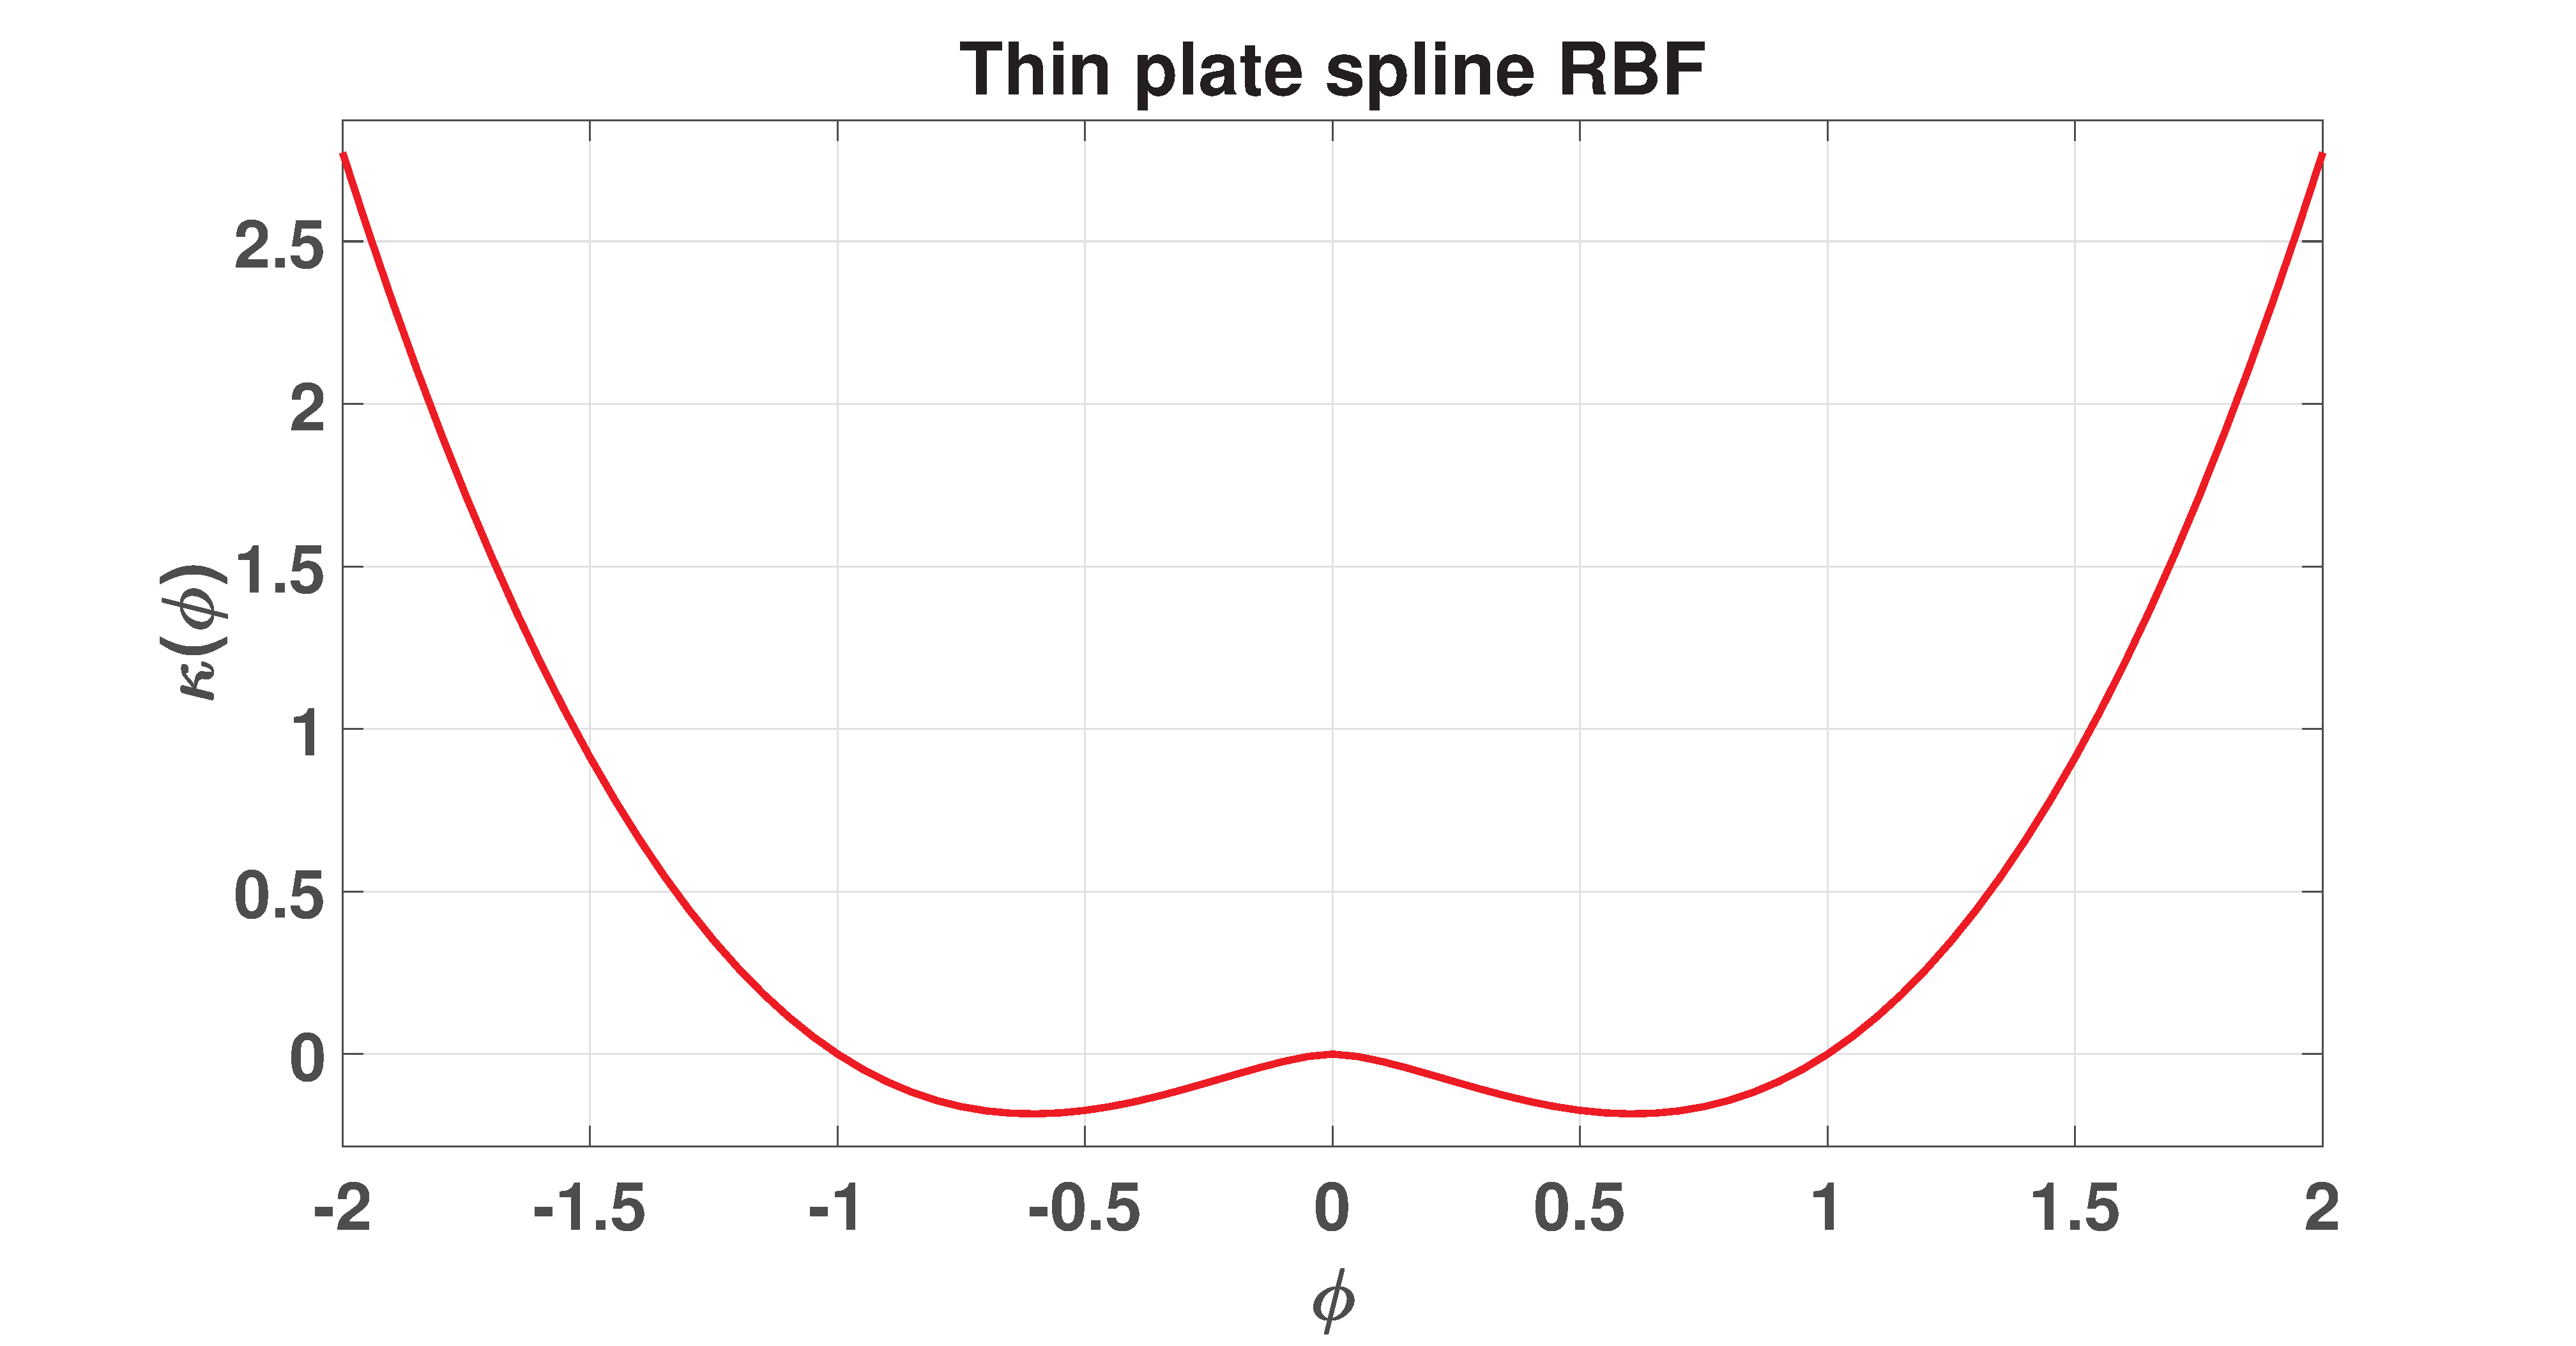
\includegraphics[width=0.75\linewidth]{figures/thinplate}
    \caption{Thin plate spline RBF}
    \label{fig: RBF_centres}
\end{subfigure}
\begin{subfigure}[t]{0.75\textwidth}
    \centering
    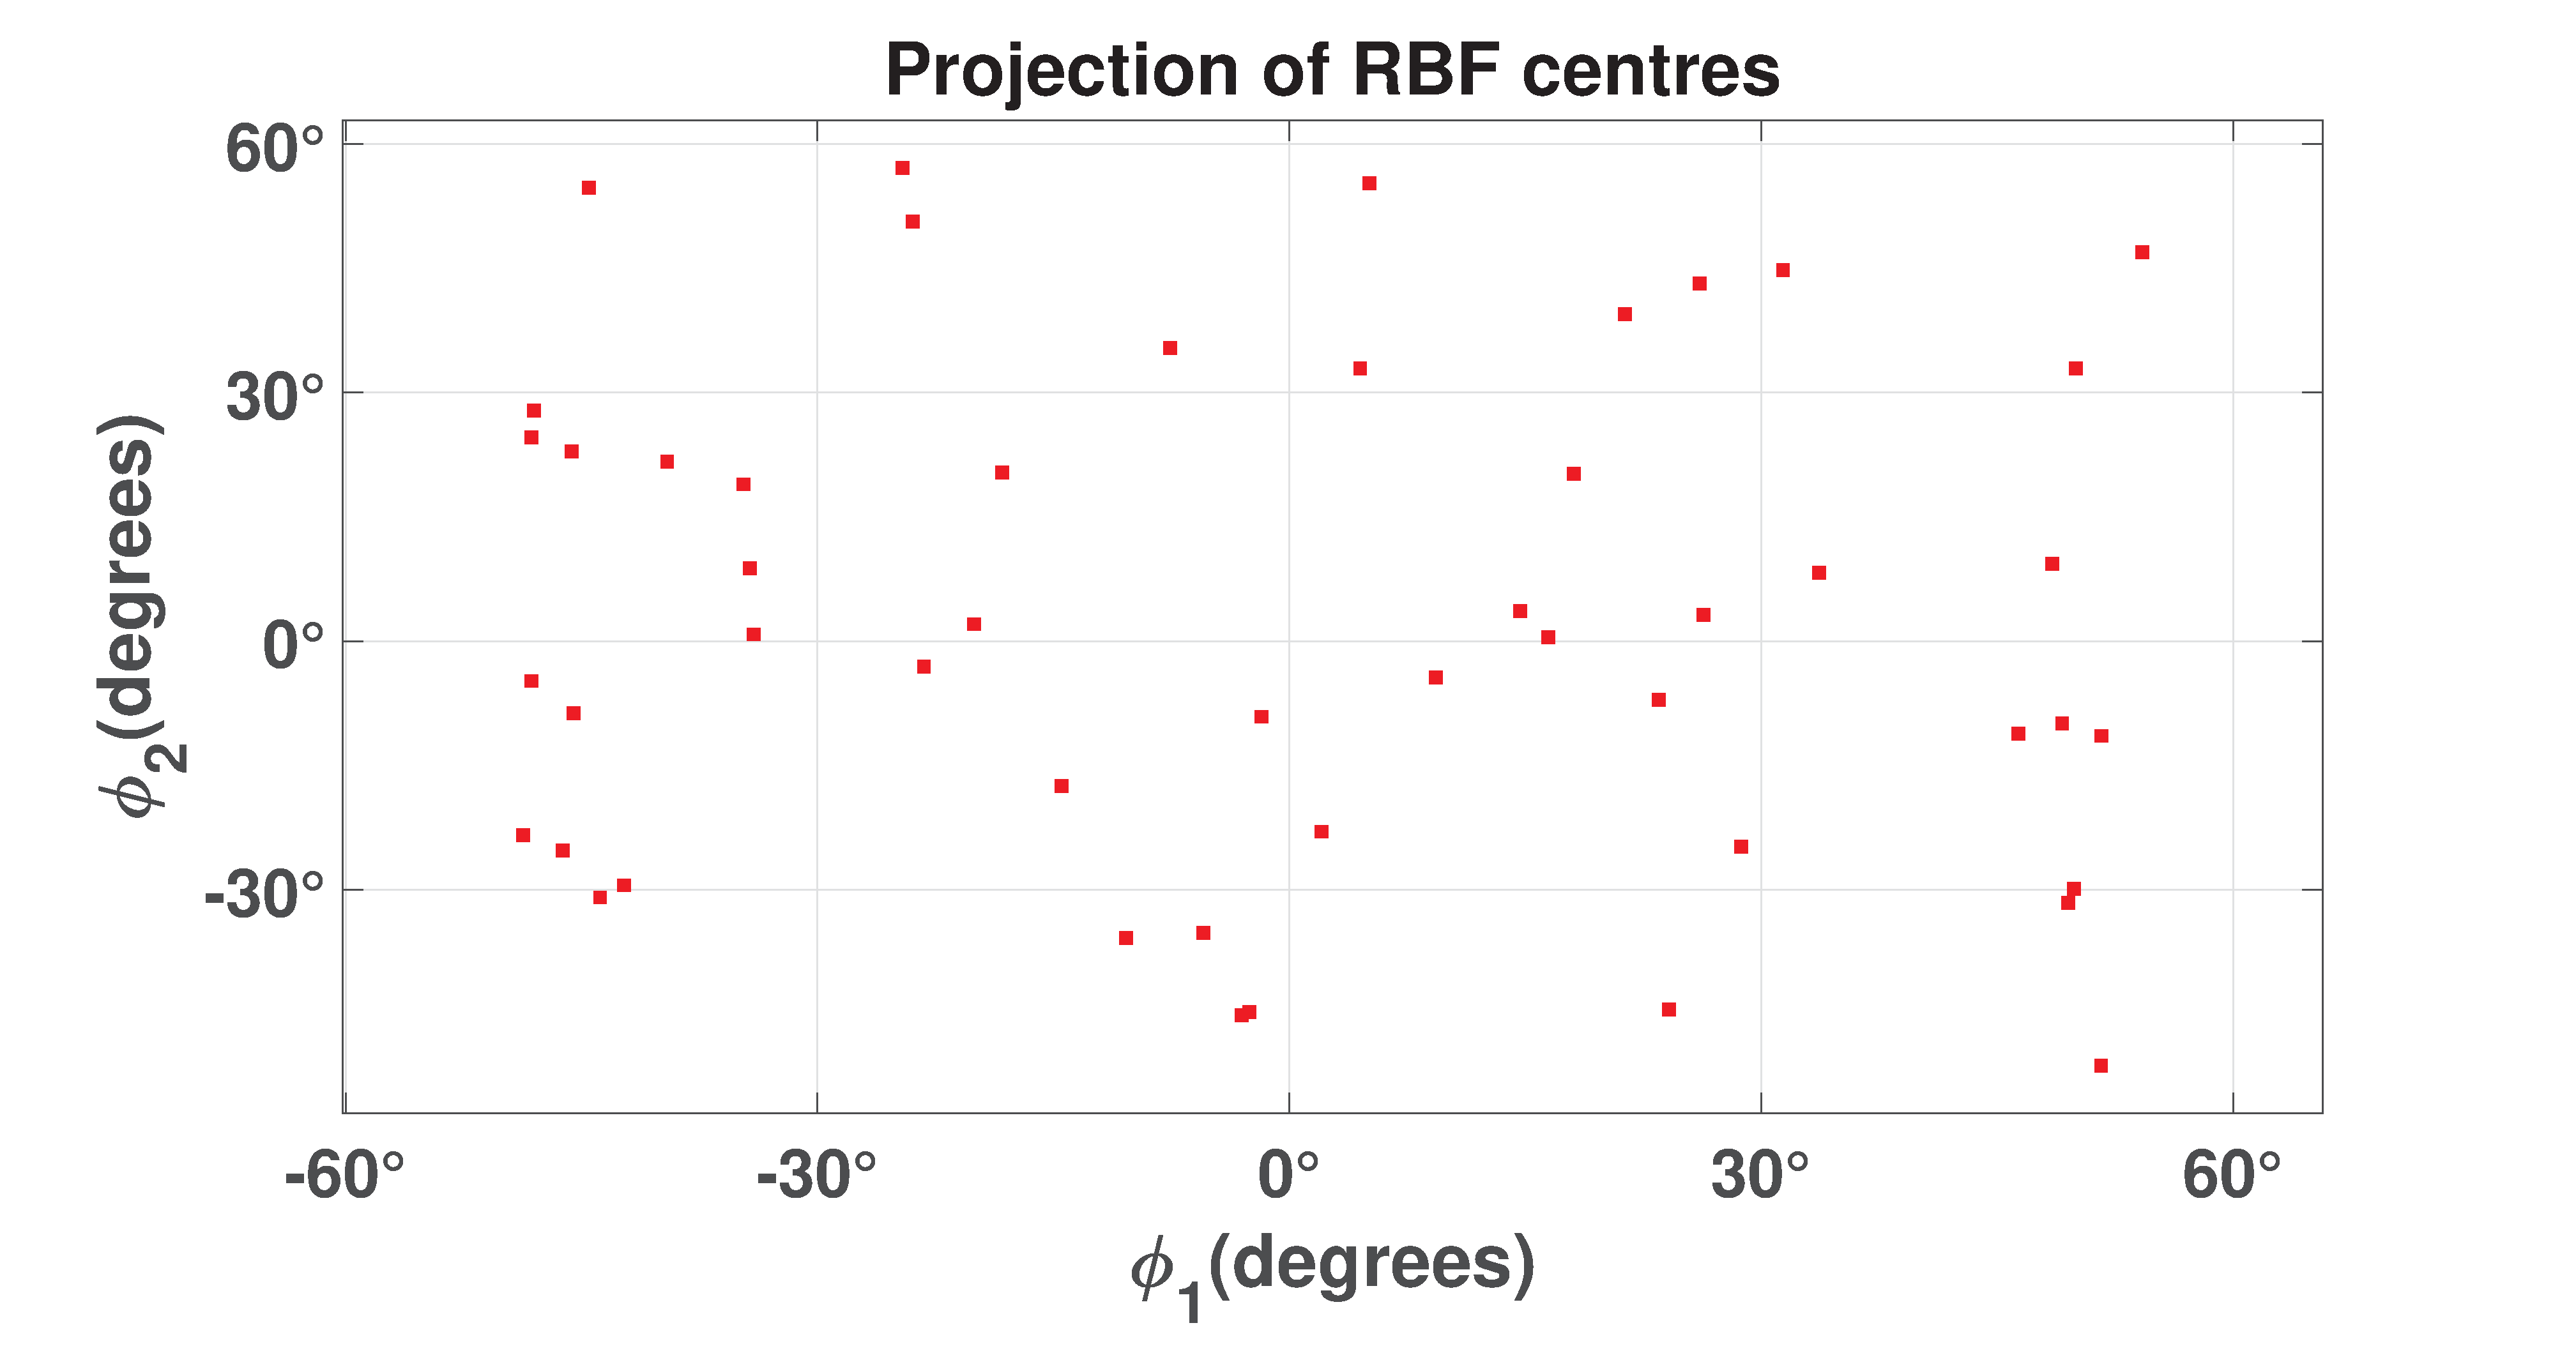
\includegraphics[width=1\linewidth]{figures/RBF_centres}
    \caption{RBF centres projected onto a plane for $\mathbf{\Psi_4}$ }
    \label{fig: thinplate}
\end{subfigure}
\caption{Thin plate splines RBF and the centres}
\end{figure}


}		% Plant
	{\section {Der wissenschaftliche Schreibstil}
\label{a:stil}

Die nachfolgenden Unterpunkte sind dem an der Universität Essen
entwickelten Schreibtrainer entnommen, \cite{BuBiPo00}. Dort kann
ein Vielfaches an Informationen mehr rund um das Schreiben
nachgeschlagen werden, was bitte als Ermunterung verstanden werden
soll! Im Internet findet man den Schreibtrainer unter der
Web-Adresse

\begin{center}
\href{http://www.uni-essen.de/schreibwerkstatt/trainer}
{http://www.uni-essen.de/schreibwerkstatt/trainer}.
\end{center}


\subsection{Korrektheit}

Der sprachliche Ausdruck sollte so treffend wie möglich sein. Die
Wörter dürfen weder umgangssprachlich noch Modewörter oder
Füllwörter sein, hier können Wörterbücher eine Hilfe sein.

Die Regeln der Grammatik, der Rechtschreibung und der
Zeichensetzung sind zu beachten. Texte, Sätze oder Wörter, die
sprachlich falsch sind, können für den Leser missverständlich oder
ärgerlich sein. Die Sätze in Schrifttexten müssen vollständig
sein.

Dass die eigentlichen Ergebnisse (z.B.\ Experimente) auch korrekt
wiedergegeben werden müssen (auch wenn es nicht so schön aussieht,
wie eigentlich erwartet), ist selbstverständlich. Wer hier nicht
wahrhaftig ist, schadet nicht nur sich selbst, sondern in gewisser
Weise der ganzen Weiterentwicklung.


\subsection{Verständlichkeit}

Nicht alles, was richtig ist, ist auch  verständlich. Die
Verständlichkeit eines Textes muss aus der Perspektive des Lesers
beurteilt werden: Seine Position, sein Vorwissen, sein
Aufnahmevermögen sind zu bedenken. Formulierungen sollten so genau
wie möglich, aber nicht genauer als nötig sein. Entsprechend sind
\begin{itemize}
    \item solche Wörter zu wählen, die bekannt sind;
    \item vermutlich unbekannte, klärungsbedürftige Wörter so einzubinden,
        dass ihre Bedeutung sich aus dem Zusammenhang erschließt,
        sie zu definieren oder zu erklären;
    \item Sätze weder nebeneinander zu stellen noch zu verschachtelt zu bauen und
    \item abhängig von der Textsorte und der Länge des Textes Textkommentare einzufügen.
\end{itemize}


\subsection{Argumentationweise}

Der Gang einer Argumentation ist immer vom Thema und von der
Textsorte abhängig. Um zunächst einen groben Textverlauf
festzulegen, sollte man die folgenden sechs Fragen klären:

\begin{enumerate}
    \item Was ist das Textziel?
    \item Was ist der Textinhalt? Was wird warum eingegrenzt?
    \item Was gehört nicht (mehr) zum Textinhalt, was wird ausgegrenzt?
    \item Welche Teile des Textinhaltes gehören wie zusammen, wie ist die
        Struktur des Themas?
    \item Welcher Teil des Textinhalts ist ein geeigneter Zielpunkt?
    \item Welcher Teil des Textinhalts ist ein geeigneter
        Anfangspunkt?
\end{enumerate}

Die sechs Fragen skizzieren die Möglichkeiten, die für eine
Argumentation bestehen, sie legen den roten Faden fest. Sie zeigen
deutlich, dass - selbst bei übereinstimmender Textsorte und
übereinstimmendem Textziel - viele unterschiedliche Texte
(Textverläufe) zu einem Thema denkbar sind. Um sich bewusst für
einen Verlauf entscheiden zu können, ist es wichtig, das Thema und
damit auch den Textinhalt genau zu analysieren.


\subsection{Quellenangaben}


Mit der wichtigste Unterschied zwischen wissenschaftlicher
Schreibpraxis und dem Verfassen von anderen Texten ist die
detaillierte Angabe der geistigen Quellen Ihrer eigenen Arbeit.
Sie werden in der Anfangsphase der Arbeit ja diverse Bücher,
Artikel, Konferenzbeiträge, Handbücher, etc.\ gelesen haben.
Manche stellen sich als belanglos für Ihrer Arbeit heraus, aus
anderen ergeben sich Ihre wesentlichen Ideen.

Grundsätzlich sind Sie dazu verpflichtet, all diese Quellen
aufzuführen und die Stellen in Text zu markieren, die auf den
Ergebnissen anderen beruhen (evtl.\ auch Ihren eigenen, falls Sie
schon Veröffentlichungen gemacht haben, können Sie auch diese
zitieren).

Das Zitat wird meist an einen Satz mit Komma angehängt, wobei in
der Regel in den Ingenieurswissenschaften nicht wörtliche Zitate,
die man dann noch durch Hervorhebung kennzeichnen sollte, genutzt
werden, sonderen die Umschreibung des Inhaltes in eigenen Worten
erfolgt, was den Text dann verständlicher machen sollte.

Das Literaturverzeichnis befindet sich nach dem Schluss und vor
dem Anhang. Hier werden alle Literaturstellen aufgeführt. \LaTeX
bietet hier viele Möglichkeiten der Automation, die im nächsten
Kapitel noch genauer beschrieben werden.

\subsection{Struktur}


Jede schriftliche wissenschaftliche Arbeit beginnt mit einer
Einleitung. Diese Einleitung
\begin{itemize}
    \item führt in den abzuhandelnden Themenbereich ein,
    \item benennt das Thema,
    \item erörtert die zu behandelnde Fragestellung,
    \item erläutert die Zielsetzung,
    \item beschreibt die Vorgehensweise und
    \item skizziert den Aufbau der Arbeit.
\end{itemize}

Bitte bedenken Sie, dass es Leser gibt, die ausschließlich die
Einleitung und den Schluss (Zusammenfassung und Ausblick) lesen
und Ihre Arbeit diesen Lesern alle notwendigen Informationen in
diesen Kapiteln zur Verfügung stellen muss, damit diese beurteilen
können, ob die Arbeit überhaupt das Gesuchte enthält und ob ein
Lesen des Hauptteils wirklich die erwarteten Erkenntnisse bringt.
Tipp: Betrachten Sie Arbeiten anderen Autoren unter diesem
Gesichtspunkt!

Der Hauptteil ist ebenfalls strukturiert aufzubauen, hier gibt es
allerdings keine allgemeingültigen Gesetze. In Abhängigkeit davon,
ob Sie eher theoretisch, methodisch oder experimentell gearbeitet
haben werden Sie die Reihenfolge der Kapitel auswählen. Bitte
überlegen Sie sich eine Gewichtung der Kapitel, die sich dann im
Umfang wiederspiegeln sollte und nicht immer proportional zu dem
Arbeitsaufwand für das einzelne Problem ist. Z.B.\ kann Sie die
Fehlersuche in einem Programm Wochen gekostet haben, die Sie aber
bitte nicht in epischer Breite beschreiben!


Im Schlussteil steht eine Zusammenfassung der Arbeitsergebnisse.
Bitte schauen Sie sich dazu auch die Problemstellung, die Sie in
der Einleitung formuliert haben noch einmal unter dem Aspekt an,
ob Sie Divergenz feststellen. Bitte bringen Sie keine noch nicht
erwähnten Erkenntnisse, Messungen, Methoden in der Zusammenfassung
unter, alles muss schon im Hauptteil beschrieben sein.

Als letztes folgt der Ausblick, der mögliche Anschlussprojekte,
unbeantwortete Fragestellungen, genauer zu betrachtende Themen
aufführt. Scheuen Sie sich nicht, dort die Punkte zu nennen, die
Ihnen während Ihrer Arbeit in den Sinn gekommen sind. Eine gute
Arbeit zeichnet sich nicht zuletzt dadurch aus, dass sie mehr
Fragen aufwirft als klärt!!
} 	        %
% 	%
	\ifthenelse{\equal{\isenglish}{true}}%
	{\section{Controller Design}
\label{Chapter:Cont}
This section discusses the theoretical background of controllers relevant for this thesis work in brief. An overview of related topics such as energy-based swing-up control, the linear quadratic regulator (LQR) and model predictive control (MPC) is presented.
% 
% 
\subsection{Swing-up Control}
\label{sec: swingup}
The swing-up control problem for the ADIP is to swing the system (the arm and the pendulum) up from its stable equilibrium at $\phi_1 = \phi_2 = \pi$ rad., and balance it about its unstable equilibrium at $\phi_1 = \phi_2 = 0$. This is achieved by swinging up the system from its stable equilibrium position through a `swing-up' controller and bringing it into a \textit{basin of attraction} in the up-up configuration where the swing-up controller is switched to a locally convergent stabilizing controller, usually an LQR, that will balance the system about its up-up position. Swing-up control for inverted pendulum systems, in general, has been traditionally achieved through feedback linearization techniques \cite{Spong}, or energy-based control \cite{Cazzolato}. Though the feedback linearization technique has almost always worked perfectly well in solving the swing-up control problem, it does not come with any stability analysis or performance guarantees.\par
Fantoni et al. \cite{Fantoni} solve this issue by presenting a control strategy based on energy approach and passivity properties of the pendubot system (which is the same as ADIP). This control strategy ensures that the state is brought either arbitrarily close to the up-up position or to a homoclinic orbit that will eventually enter the basin of attraction of any locally convergent controller. Stability analysis for the same is presented based on LaSalle's theorem. The main result of the work by the authors is presented as a theorem in \cite{Fantoni}. The swing-up control law is given as:
\begin{equation}
    u = \frac{-k_DF-t_M(\dot{\phi_1}+k_P{\phi_1})}{t_Mk_E\tilde{E} + k_D\theta_2} \;,
\end{equation}
with 
\begin{align*}
F &= \theta_2\theta_3\sin{(\phi_1-\phi_2)}\dot{\phi}_2^2 + \theta_3^2\cos{(\phi_1 - \phi_2)}\sin{(\phi_1 - \phi_2)}\dot{\phi_1}^2\\
&+ \theta_2\theta_4g\sin{\phi_1} + \theta_3\theta_5g\sin{(\phi_1 - 2\phi_2)} + C_{arm}\theta_2\dot{\phi_1} + C_{pend}\theta_3\cos{(\phi_1-\phi_2)}\dot{\phi_2}\;, \\
t_M &= (\theta_1\theta_2 - \theta_3^2\cos^2{(\phi_1-\phi_2})) \;,\\
\tilde{E} &= E - E_{top}
\end{align*}
where $k_E,k_D, \textup{and}~ k_P$ are strictly positive constants and $\tilde{E}$ is the difference in the actual total energy of the system and total energy at the up-up position. The $\theta_i,~i = \{1,2,\dots,5\}$ are given in Chapter \ref{Chapter:Plant}.\\
Furthermore, Xin et al.~\cite{XIN} propose a sufficient condition for the parameters: $k_E,k_D, \textup{and}~ k_P$ in the control law such that the total energy of the Pendubot will converge to the potential energy of its top upright position. The initial parameters were obtained through the method proposed by the authors and thereafter, a GA was used to fine tune the parameters.\pagebreak

\subsection{Linear Quadratic Regulator}
\label{sec:lqr}
The overarching goal of this thesis is to reformulate strongly nonlinear dynamics in a linear framework to enable the use of powerful optimal and robust control techniques available for linear systems. Consider the nonlinear system affected by an external input:
\begin{equation}
\label{eq:statedyn}
    \frac{d}{dt}\mathbf{x}(t) = \mathbf{f}(\mathbf{x,u})\;, \quad \mathbf{x}(0) = \mathbf{x}_0 \;,
\end{equation}
with multi-channel control input $\mathbf{u} \in \mathbb{R}^q$ and continuously differentiable dynamics $\mathbf{f(x,u)}$ : $\mathbb{R}^n \times \mathbb{R}^m \rightarrow \mathbb{R}^n$. Without loss of generality, the origin is an equillibrium: $\mathbf{f(0,0) = 0}$.\\
Inifinte-horizon optimal control then minimizes the following quadratic cost functional 
\begin{equation}
\label{eq:Costfunc}
    J(\mathbf{x,u}) = \frac{1}{2}\int_0^\infty \mathbf{x}^\top (t)\mathbf{Qx}(t) + \mathbf{u}^\top\mathbf{Ru}(t)~dt
\end{equation}
with state and input weight matrices $\mathbf{Q} \in \mathbf{R}^{n\times n}$ and $\mathbb{R}^{m\times m}$. Both matrices are symmetric and fulfill $\mathbf{Q} > 0$ and $\mathbf{R} \geq 0$. A full-state feedback control law
\begin{equation}
    \mathbf{u(x)} = -\mathbf{F(x)x}
\end{equation}
with gain $\mathbf{F}: \mathbb{R}^n \rightarrow \mathbb{R}^{m\times n}$ is sought to minimize the cost function in Eq.~\ref{eq:Costfunc} subject to the state dynamics in Eq.~\ref{eq:statedyn} to drive the system to the origin, i.e. \[\lim_{x\to\infty} \mathbf{x}(t) = \mathbf{0} \quad \forall ~\mathbf{x}.\]  
The above control problem simplifies considerably for linear systems of the form
\begin{equation}
    \frac{d}{dt}\mathbf{x}(t) = \mathbf{Ax} + \mathbf{Bu}, \quad \mathbf{x}(0) = \mathbf{x}_0.
\end{equation}
Using $\mathbf{z} = \mathbf{x}^\top\mathbf{Px}$ for the co-state, the optimal control is given by
\begin{equation}
    \mathbf{u} = \mathbf{-R}^{-1}\mathbf{B}^\top\mathbf{z} = \mathbf{-R}^{-1}\mathbf{B}^\top\mathbf{Px} \;, 
\end{equation}
with constant gain $\mathbf{F} = \mathbf{-R}^{-1}\mathbf{B}^\top\mathbf{P}$ and where the semi-definte matrix $\mathbf{P} \in \mathbb{R}^{n \times n}$ is the solution to the algebraic Riccati equation (ARE):
\begin{equation}
    \mathbf{Q} + \mathbf{PA} +\mathbf{A}^\top\mathbf{P} - \mathbf{PBR}^{-1}\mathbf{B}^\top\mathbf{P} = \mathbf{0}\;.
\end{equation}
The above formulation is referred to as the linear quadratic regulator for which the solution of ARE yields a global state-feedback control law. This simplicity motivates efforts to find linear representations for nonlinear systems and explains why nonlinear embeddings via Koopman operator theory are so appealing \cite{kaiser2020datadriven}. 
\pagebreak
\subsection{Model Predictive Control}
\label{sec: MPC}
Model predictive control~(MPC) is an advanced method of feedback control that is used to control a system while satisfying a set of constraints on the input and/or the state. It offers several advantages over the infinite horizon LQR; to list a few, the input is computed over a receding finite time horizon, i.e., at each time step, an optimal control input vector is computed by minimizing a user-specified cost function (e.g., energy or tracking error) over a predefined time horizon $N_p$, and only the first value of this input vector is applied to progress the system to the next time step where the entire process is repeated, thereby enabling optimal tracking of the reference trajectory.  Although this appears as a computationally expensive process, which it is when compared to the LQR, it performs a whole lot better in the event of any external disturbances or sudden changes in reference trajectory. This is especially advantageous in tracking problems where the controller is able to `predict' any setpoint changes and react accordingly. Consequently, this also means that the controller can predict and provide early warnings of any potential problems. Also, any constraints on input and output can be imposed in a simple way in this technique.\par
For this thesis, the state-space form of MPC is considered. There is abundant literature available describing the construction and implementation of the MPC; the reader is encouraged to refer \cite{MPCbook} for a detailed explanation of the MPC. This section will therefore only briefly explain the cost function used in this thesis and an approach explored in Korda et al. \cite{MPC_Korda} to eliminate the dependence of the cost function on the dimension of state of the system which will eventually prove useful for formulating the MPC for high-dimensional systems. \par 
The following formulations are an adaptation of the formulations presented in \cite{MPC_Korda}.\\
Assume a nonlinear system of the form $\mathbf{x}_{k+1} = f(\mathbf{x}_k,\mathbf{u}_k)$ can be approximated in terms of a linear model of the form,
\begin{equation}
\label{eq:MPCdisc}
    \mathbf{x}_{k+1} = \mathbf{Ax}_k + \textbf{Bu}_k \:,
\end{equation}
The model predictive controller solves at each time step $k$ of the closed-loop iteration the optimization problem, 
\begin{equation}
  \label{eq:MPCoptim}
  \begin{alignedat}{3}
&\min_{\mathbf{u}_{i},\mathbf{x}_{i}} && J\left((\mathbf{u}_{i})_{i=0}^{N_p-1}, (\mathbf{x}_{i})_{i=0}^{N_p-1}\right) && \\
&\textup{subject to} \quad &&\mathbf{x}_{i+1}  = \mathbf{Ax}_{i} + \textbf{Bu}_{i} \:, && i = 0,1,\dots,N_p-1\\
& &&\mathbf{E}_{i}\mathbf{x}_{i} + \mathbf{F}_{i}\mathbf{u}_{i} \leq \mathbf{b}_{i} \;, &&  i = 0,1,\dots,N_p-1\\
& &&\mathbf{E}_{N_p}\mathbf{x}_{N_p} \leq \mathbf{b}_{N_p} \;, &&\\
&\textup{parameter} && \mathbf{x}_0 = \mathbf{x}_k \;, &&   
\end{alignedat}
\end{equation}

where the matrices $\mathbf{E}_{i} \in \mathbb{R}^{n_c \times n}$, $\mathbf{F}_{i} \in \mathbb{R}^{n_c \times m}$ define the state and input polyhedral constraints, respectively and $\mathbf{b}_{i} \in \mathbb{R}^{n_c}$ is the vector of constraints, and the convex quadratic cost function $J$ is given by,
\begin{equation}
\label{eq:MPCcostfunction}
    J = \mathbf{x}_{N_p}^\top \mathbf{Q}_{N_p} \mathbf{x}_{N_p} + \sum_{i=0}^{N_p-1} \mathbf{x}_{i}^\top \mathbf{Q} \mathbf{x}_{i} + \mathbf{u}_{i}^\top \mathbf{R}\mathbf{u}_{i} \;,
\end{equation}
% 
where $\mathbf{x}_{N_p}$ is the final state at time instance $N_p$, $\mathbf{Q}_{N_p} \in \mathbb{R}^{n \times n}$ is the corresponding penalty on the final state.
\par 
The optimization problem (\ref{eq:MPCoptim}) parametrized by the current state of the nonlinear dynamical system $\mathbf{x}_k$ then defines a feedback controller $F\mathbf{(x)} = \mathbf{u_0}^\ast(\mathbf{x}_k)$, where $\mathbf{u_0}^\ast(\mathbf{x}_k)$ is the optimal solution to the optimization problem.\par
It is always beneficial to eliminate the dependence of the optimization problem on the dimension of the state $n$. Consequently, the computational complexity of solving the optimization problem will be rendered independent of the dimension $n$. This is especially useful when dealing with the approximation of nonlinear systems through the Koopman operator theory, where the state might be $\textit{lifted}$ to a higher dimension which results in a linear dynamical system that approximates the nonlinear dynamical system. This elimination can be achieved by formulating the dynamics in the following way: consider the discrete-time or the \textit{one step-ahead predictor} state-space model
\begin{align}
\label{Eq: predicteqns}
\begin{split}
    \mathbf{x}_{k+1} &= \mathbf{Ax}_k + \mathbf{B}\mathbf{u}_k \quad \quad \mathbf{x}(0) = \mathbf{x}_0\;, \\
    \mathbf{y}_k &= \mathbf{C}\mathbf{x}_k \;,
\end{split}
\end{align}
where $\mathbf{x}_{k+1} \in \mathbb{R}^{n}$ is the `future' value of the current state $\mathbf{x}_k$ at a time instance $k = [0,1,2,\dots,N_p-1]$, $\mathbf{u}_k \in \mathbb{R}^m$ is the input at time instance $k$ and $\mathbf{A} \in \mathbb{R}^{n\times n},\mathbf{B} \in \mathbb{R}^{n \times m} ~ \textup{and}~ \mathbf{C} \in \mathbb{R}^{l \times n} $ are the system, input and output matrices, respectively. Naturally, the state at time instance $k+2$ can then be predicted from Eq.~\ref{Eq: predicteqns} as
% 
\begin{equation}
\label{eq:predicteqns2}
    \mathbf{x}_{k+2} = \mathbf{Ax}_{k+1} + \mathbf{B}\mathbf{u}_{k+1} \;,
\end{equation}
% 
Subsituting Eq.~\ref{Eq: predicteqns} in Eq.~\ref{eq:predicteqns2}, the future state at the second time instance can be obtained in the terms of the initial state $\mathbf{x}_k$ as
% 
\begin{equation}
    \mathbf{x}_{k+2} = \mathbf{A}^2\mathbf{x}_{k} + \mathbf{AB}\mathbf{u}_{k} + \mathbf{B}\mathbf{u}_{k+1} \;.
\end{equation}
% 
The one-step ahead predictor model therefore, can be used recursively to predict the evolution of state for the next $N_p$ steps of interest where $N_p$ is the time interval over which a cost function is evaluated to compute the optimal input corresponding to the desired state evolution in that time interval.
% 
\begin{equation}
\label{eq: Nstep}
    \underbrace{\begin{bmatrix}
    \mathbf{x}_{k+1} \\
    \mathbf{x}_{k+2}\\
    \vdots\\
    \mathbf{x}_{k+N_p} 
    \end{bmatrix}}_{\mathbf{X}_{k+1}} = \underbrace{\begin{bmatrix}
    \mathbf{A}\\
    \mathbf{A}^2\\
    \vdots\\
    \mathbf{A}^{N_p}
    \end{bmatrix}}_{\mathbf{\bar{A}}}~\mathbf{x}_k + \underbrace{\begin{bmatrix}
    \mathbf{B} & \mathbf{0} & \dots & \mathbf{0}\\
    \mathbf{AB} & \mathbf{B} & \dots & \mathbf{0}\\
    \vdots & \vdots & \dots & \vdots\\ 
    \mathbf{A}^{N_p-1}\mathbf{B} & \mathbf{A}^{N_p-2}\mathbf{B} & \dots & \mathbf{B}\\
    \end{bmatrix}}_{\mathbf{\bar{B}}} ~ \underbrace{\begin{bmatrix}
    \mathbf{u}_k \\
    \mathbf{u}_{k+1}\\
    \vdots\\
    \mathbf{u}_{k+N_p-1}
    \end{bmatrix}}_{\mathbf{U}_k}\;.
\end{equation}
% 
Eq.~\ref{eq: Nstep} can be compactly written as,
% 
\begin{equation}
    \label{eq:NstepComp}
    \mathbf{X}_{k+1} = \mathbf{\bar{A}x}_k + \mathbf{\bar{B}}\mathbf{U}_k \;,
\end{equation}
% 
where $\mathbf{X}_{k+1} \in \mathbb{R}^{N_pn}$ is the vector of state predictions, $\mathbf{\bar{A}} \in \mathbb{R}^{N_pn\times n}$, $\mathbf{\bar{B}} \in \mathbb{R}^{N_pn\times N_pn}$ is a Toeplitz matrix~(or a diagonal-constant matrix) and $\mathbf{U}_k \in \mathbb{R}^{N_pm}$ is the vector of predicted sequence of control inputs. Note that Eq.~\ref{eq:NstepComp} depends only on the initial state $\mathbf{x}_0$ and the sequence of control inputs $\mathbf{U}_k$.\par
Consequently, the output equation is
% 
\begin{equation}
\label{eq:Nstepout}
    \mathbf{Y}_{k+1} = \mathbf{\bar{C}}\mathbf{\bar{A}x}_k + \mathbf{\bar{C}}\mathbf{\bar{B}U}_k \;, 
\end{equation}
% 
where $\mathbf{Y}_{k+1} \in \mathbb{R}^{N_pl}$ is the vector of predicted future outputs and $\mathbf{\bar{C}} \in \mathbb{R}^{N_pl\times N_pn}$ is the computed as the Kronecker product $\mathbf{I}_{N_p} \otimes \mathbf{C}$. Note that the notations used in this section, $\mathbf{\bar{A},\bar{B},\bar{C}}$ correspond to the notations $\mathbf{A_b, B_b, C_b}$ used in the Matlab script.
\par
It is then possible to transform the optimization problem (\ref{eq:MPCoptim}) to the so-called \textit{dense form}
\begin{equation}
\label{eq:MPCdense}
\begin{alignedat}{2}
        &\min_{\mathbf{U} \in \mathbb{R}^{mN_p}} \quad && \mathbf{U}^\top\mathbf{H}\mathbf{U} +  \mathbf{x}_0^\top\mathbf{G}\mathbf{U} \\
        & \textup{subject to}\quad && \mathbf{L}\mathbf{U} + \mathbf{M}\mathbf{x}_0 \leq \mathbf{c} \\
        ~ & \textup{parameter} && \mathbf{x}_0 = \mathbf{x}_k
        % \mathbf{h}^\top\mathbf{U} +
\end{alignedat}    
\end{equation}
for some positive-definite matrix, the \textit{Hessian} $\mathbf{H} \in \mathbb{R}^{mN_p \times mN_p}$ and some matrices, $\mathbf{G} \in \mathbb{R}^{n \times mN_p}$, $\mathbf{L} \in \mathbb{R}^{n_cN_p \times mN_p}$, $\mathbf{M} \in \mathbb{R}^{n_cN_p \times n}$ and vector of constraints $\mathbf{c} \in \mathbb{R}^{n_cN_p}$. The matrices are defined as
\begin{equation}
    \begin{alignedat}{5}
    &\mathbf{H} && = \mathbf{\bar{R}} + \mathbf{\bar{B}}^\top\mathbf{\bar{Q}}\mathbf{\bar{B}} \;, \quad &&\mathbf{G} && = 2\mathbf{\bar{A}}^\top\mathbf{\bar{Q}}\mathbf{\bar{B}}\;, && \\
    & \mathbf{L} &&= \mathbf{\bar{F}} + \mathbf{\bar{E}\bar{B}}\;, && \mathbf{M} && = \mathbf{\bar{E}\bar{A}} \;,&& \mathbf{c} &&= [\mathbf{b}_0^\top,\dots,\mathbf{b}_{N_p}^\top]^\top
    % \mathbf{h} &&= \mathbf{\bar{B}}^\top\mathbf{q} + \mathbf{r} \;, \quad && 
    \end{alignedat}
\end{equation}
where $\mathbf{\bar{Q}} = \mathbf{I}_{N_p} \otimes \mathbf{Q}  ~\in \mathbb{R}^{nN_p \times nN_p}$, $\mathbf{\bar{R}} = \mathbf{I}_{N_p} \otimes \mathbf{R} ~ \in \mathbb{R}^{N_pm \times N_pm}$, $\mathbf{E} = \mathbf{I}_{N_p} \otimes \mathbf{E}  ~\in \mathbb{R}^{n_cN_p \times n_cN_p}$, and
\begin{equation*}
    \mathbf{\bar{F}} = \begin{bmatrix}
    F_0 & 0 & ~ \dots ~ & 0 \\
    0 & F_1 & ~ \dots ~ & 0 \\
    \vdots & \vdots & & \vdots\\
    0 & 0 & ~ \dots ~ & F_{N_p-1}\\
    0 & 0 & ~ \dots ~ & 0
    \end{bmatrix}
\end{equation*}
Note that (\ref{eq:MPCdense}) is formulated in a purely quadratic form and one can use any of the available QP solvers available. The optimization is done over the predicted control inputs $\mathbf{U} = [\mathbf{u}_0^\top,\mathbf{u}_1^\top,\dots,\mathbf{u}_{N_p-1}^\top]^\top$. Importantly, note that the size of the $\mathbf{H}$ and that of the vector of constraints $\mathbf{c}$ is independent of the dimension of the state. This formulation, when extended to lifted systems with a lifted dimension $K$ of the state, proves very useful as the above said matrices are independent of $K$ and the matrices can, in fact, be precomputed offline before deploying the controller. One needs only to evaluate the nonlinear mapping or the lifting of state at each time step, thereby making the cost of computation inexpensive. In summary, once the data matrices in (\ref{eq:MPCdense}) are formed, the cost of solving the optimization problem is independent of the dimension of the state space and therefore, a nonlinear MPC problem can be solved as a linear MPC problem provided linear predictors of the form (\ref{eq:MPCdisc}) can be estimated using the Koopman operator theory. Section \ref{Chapter:Data} deals with such \textit{lifting} variables that can approximate nonlinear systems.
% It is possible to write the discrete-time version of the regulation cost function in Eq.~\ref{eq:Costfunc} over a finite horizon $N_p$ as
% % 
% \begin{equation}
%     J_p = \sum_{i=0}^{N_p-1} \mathbf{x}_{k+i}^\top \mathbf{Q} \mathbf{x}_{k+i} + \mathbf{u}_{k+i}^\top \mathbf{R}\mathbf{u}_{k+i}
% \end{equation}
% % 
% which can be written as,
% \begin{equation}
%     J_p = \mathbf{X}_{k}^\top \mathbf{\bar{Q}} \mathbf{X}_{k} + \mathbf{U}_{k}^\top \mathbf{\bar{R}}\mathbf{U}_{k} \;, \quad \quad k = [0,1,\dots,N_p-1]
% \end{equation}
% . This can further be formulated in a pure quadratic form by considering $\mathbf{w} = [\mathbf{X}_k\quad \mathbf{U}_k]^\top$ which results in
% % 
% \begin{equation}
%     J_p = \mathbf{W}^\top\begin{bmatrix}
%     \mathbf{\bar{Q}} & \\
%      & \mathbf{\bar{R}}
%     \end{bmatrix} \mathbf{W}
% \end{equation}
% % 
% The optimal control problem (OCP) for a LTI predictive control law can then defined as
% % 
% \begin{align}
% \label{eq:MPC1}
% \begin{split}
%     & \min_{\mathbf{U}_k} \mathbf{W}^\top\begin{bmatrix}
%     \mathbf{\bar{Q}} & \\
%      & \mathbf{\bar{R}}
%     \end{bmatrix} \mathbf{W} \;, \\
%     & \textup{subject to}\\
%     &\tilde{\mathbf{A}}\mathbf{W} + \tilde{\mathbf{b}} = \mathbf{0}\;, \\
%     &\textup{with}\\
%     &\tilde{\mathbf{A}} = [(\mathbf{\bar{A}} - \mathbf{I}) \quad \mathbf{\bar{B}}] ~ \textup{and} ~ \tilde{\mathbf{b}} = \mathbf{A}_0\mathbf{x}
% \end{split}
% \end{align}
% The Eqs.~\ref{eq:NstepComp} and \ref{eq:Nstepout} can be written in a quadratic form  and the optimization can be formulated as minimization of 



% % 
% where $\mathbf{Q} \in \mathbb{R}^{l\times l}$ is the penalty on the output state error and is positive semi-definite and $\mathbf{R} \in \mathbb{R}^{m\times m}$ is the penalty on the input and is positive definite. This is similar to the cost function defined in Eq. \ref{eq:Costfunc} except that the cost function here is evaluated over a finite time horizon defined by $N_p$ time steps. The cost function for the entire prediction horizon can consequently be written as,
% % 
% \begin{equation}
% \label{eq:MPC2}
%     \mathbf{J}_p = (\mathbf{R}_{k+1} - \mathbf{Y}_{k+1})^\top\mathbf{\bar{Q}}(\mathbf{R}_{k+1} - \mathbf{Y}_{k+1})^\top + \mathbf{U}_k^\top\mathbf{\mathbf{R}}\mathbf{U}_k \;, 
% \end{equation}\\
% % 
%  and is not to be confused with $\mathbf{R} = \mathbf{I}_{N_p} \otimes \mathbf{r} ~\in \mathbb{R}^{N_pl}$ which is the vector of reference trajectory. Substituting Eqs.~\ref{eq:NstepComp} and \ref{eq:Nstepout} in Eq.~\ref{eq:MPC2} and after some algebraic manipulations and taking the gradient of the cost function with respect to the optimization variable $\mathbf{U}_k$ and solving for the optimal control sequence $\mathbf{U}_k^{\ast}$ by setting the gradient to zero,  which is elaborately explained in \cite{MPCbook}, the final result can be presented as,
% % 
% \begin{equation}
%     \mathbf{U}_k^{\ast} = -(\mathbf{\bar{B}}^\top\mathbf{\bar{C}}^\top\mathbf{\bar{Q}}\mathbf{\bar{C}}\mathbf{\bar{B}} + \mathbf{\bar{R}})^{-1}~(\mathbf{\bar{B}}^\top\mathbf{\bar{C}}^\top\mathbf{\bar{Q}}^\top\mathbf{\bar{C}}\mathbf{\bar{A}}\mathbf{x}_k - \mathbf{\bar{B}}^\top\mathbf{\bar{C}}^\top\mathbf{\bar{Q}}^\top\mathbf{R}_{k+1}) \;.
% \end{equation}
% % 
% The above optimal control input sequence can be computed without any significant computational effort. However, the significance of MPC relies just not on the predictive capability but also on the ease of including constraints on the inputs and outputs.

% The general structure of the controller is shown below. 
% \begin{equation}
%     J = \sum_{i=0}^{N_p-1} \boldsymbol{e}_{k+i}^\top \mathbf{Q} \boldsymbol{e}_{k+i} + \boldsymbol{\Delta}\mathbf{u}_{k+i}^\top \mathbf{R}\boldsymbol{\Delta}\mathbf{u}_{k+i} \;, 
% \end{equation}
% where $\boldsymbol{e_{k+i}} = \mathbf{x}_{k+i} - \boldsymbol{r}_{k+i}$ is the deviation of the state from its reference, $\boldsymbol{\Delta}\mathbf{u}_{k+i}$ is the input increment and $N_p$ is the prediction horizon,  The model in -- needs to be augmented with the incremental value of input
% \begin{equation}
% \label{eq:MPCmodel}
%     \begin{bmatrix}
%     \mathbf{x}_{k+1} \\ \mathbf{u}_k
%     \end{bmatrix} = \begin{bmatrix}
%     \mathbf{A} & \mathbf{B} \\ \mathbf{0} & ~\mathbf{I}_m
%     \end{bmatrix}~\begin{bmatrix}
%     \mathbf{x}_k \\ \mathbf{u}_{k-1}
%     \end{bmatrix}~+~ \begin{bmatrix}
%     \mathbf{B} \\ ~\mathbf{I}_m 
%     \end{bmatrix} \boldsymbol{\Delta}\mathbf{u}_k \;.
% \end{equation}
% \textbf{Topics to be included in this section:}
% $\boldsymbol{e_{k+i}} = \boldsymbol{r}_{k+i} - \mathbf{Cx}_{k+i}$ is the deviation of the output state from its reference, 
% The optimal control problem (OCP) for the LTI predictive control law is defined as
% \begin{align}
%     & \min_{\Delta \mathbf{U}_k} \sum_{i=0}^{N_p-1} \boldsymbol{e}_{k+i}^\top \mathbf{Q} \boldsymbol{e}_{k+i} + \boldsymbol{\Delta}\mathbf{u}_{k+i}^\top \mathbf{R}\boldsymbol{\Delta}\mathbf{u}_{k+i} \;, \tag{5.10a}\label{eq:MPCcost} \\
%     & \textup{subject to} \notag\\
%     & \tilde{\mathbf{x}}_{k+j+1} = \tilde{\mathbf{A}}\tilde{\mathbf{x}}_{k+j} + \tilde{\mathbf{B}}\boldsymbol{\Delta}\mathbf{u}_{k+j} \;, \tag{5.10b}\label{eq:MPCmodel_const} \\
%     & \mathbf{u}_{k+j} = \mathbf{u}_{k-1} + \sum_{i=0}^j (\boldsymbol{\Delta}\mathbf{u})_{k+i} \in \mathcal{U} \;, \tag{5.10c}\label{eq:MPCinput_const} \\
%     & \tilde{\mathbf{x}}_{k+j} \in \mathcal{X}~ \textup{for} ~j \in [0,1,\dots,N-1] \;, \tag{5.10d}\label{eq:MPCstates}
% \end{align}
% where $\mathcal{U}$ is the constrained input set and $\mathcal{M}$ is the set of admissible states. The vector $\boldsymbol{\Delta}\mathbf{U}_k = [\boldsymbol{\Delta}\mathbf{u}_k^\top,\dots,\boldsymbol{\Delta}\mathbf{u}_{k+N-1}^\top]^\top$ represents the future inputs. Note that the model constraints (\ref{eq:MPCmodel_const}) are linear in the input increments, thus they can be substituted into the cost function by using an $N$ step ahead prediction equation. This will transform the optimal control problem into a quadratic program (QP), which can be solved fast and efficiently. An important observation is that the order of the model (\ref{eq:MPCmodel}), does not increase the problem complexity since the QP only has the inputs as decision variables. 
% \begin{itemize}
%     \item Overview of control in Koopman coordinates
% \end{itemize}
}		% Controllers
	{\section {Schreiben am Institut für Regelungstechnik}
\label{a:ab_rts_en}


\subsection{Hardware-Ausstattung}

Im Rechnerraum N1.059 stehen PCs für Studenten zur Verfügung, die
generell sowohl für Berechnungen (meist mit \textsc{Matlab}/\textsc{Simulink}) als
auch für die Ausarbeitung des schriftlichen Teils genutzt werden
können.


\subsection{Verfügbare Software}

Als geeignete \LaTeX-Editoren haben sich
\begin{itemize}
    \item TeXnicCenter
    \item Texmaker
    \item TeXStudio
    \item Visual Studio Code + LatexWorkshop
\end{itemize}

bewährt.
Prinzipiell kann jeder Editor (z.B. LED) genutzt werden.
Damit haben Sie die richtigen Einstellungen zum Kompilieren und es sollte eine pdf-datei mit ihrer Arbeit erzeugt werden.
Ist dies nicht der Fall, überprüfen Sie Ihre Einstellungen, ob die Pfade zu den Programmen zur Nachbereitung und des Viewers stimmen. 

\subsection{Zitate aus der Literatur-Datenbank}

Das Institut verfügt über eine gemeinsame
Literatur-Datenbank, in der eine Vielzahl der Bücher und Artikel,
die Sie zitieren wollen, wahrscheinlich bereits enthalten sind. 
Das entsprechende bib-file, welches Sie mit Ihrem \LaTeX-Editor oder einem
Literaturverwaltungstool wie beispielsweise ''jabref'' öffnen können, 
finden Sie unter \verb"S:\ICS Library\ics.bib". 
Fragen Sie Ihren Betreuer/Betreuerin nach der aktuellsten Version und kopieren Sie diese in das Hauptverzeichnis Ihrer Arbeit.

Prüfen Sie, ob Ihre Literaturstelle enthalten ist. 
Dann können Sie einfache das \LaTeX-Kürzel in
den entsprechenden Befehl einfügen. Durch den Verweis auf die
Bib\TeX-Datei wird dann das
Literaturverzeichnis automatisch erstellt. Hierfür müssen Sie \texttt{biber} aufrufen.

Sollte das von Ihnen gewünschte Zitat noch nicht in der
Literaturdatenbank aufgeführt sein, sprechen Sie bitte mit Ihrem
Betreuer. Wir sind bemüht, die Datenbank um für uns wichtige
Dokumente zu erweitern und die Tatsache, dass die Literaturstelle
von Ihnen ausgewählt wurde, spricht schon für die Wichtigkeit! Wir
werden das dann in der Regel übernehmen und somit können Sie auch
''Ihr'' Zitat dann in der Datenbank finden. Es empfiehlt sich, die
Literaturliste bereits bei Beginn der Niederschrift mit dem Stand
der Datenbank zu vergleichen, damit zusätzliche Einträge oder
Änderungen nicht in letzter Minute noch eingepflegt werden müssen.
Es ist immer Hilfreich dem Betreuer vollständige Angaben zur Literaturstelle
zu machen: Titel, Autoren, Datum, DOI, vielleicht sogar ein PDF!


\subsection{Binden der Arbeit}

Am Arbeitsbereich gibt es die Möglichkeit, die fertige Arbeit zu drucken und zu
binden. Dazu fertigt man in der Regel drei Exemplare an (für den
Betreuer, den Professor und sich selbst), ggf.\ aber auch mehr.
Nachdem der Titel der Arbeit endgültig festgelegt ist, wird dieser
von Ihrem Betreuer in die Literaturdatenbank des Arbeitsbereiches
eingetragen. 

Ihre Arbeit wird in der korrekten Reihenfolge gedruckt. Vorne kommt eine Klarsichtfolie davor und dahinter eine Kartonseite.

Im Gegensatz zu einer Leimbindung, die auf den ersten Blick sehr
elegant aussieht, hat die Klammerbindung den unschätzbaren
Vorteil, dass sie auch nach Jahren nicht auseinander fällt. Suchen
Sie sich die Klammern in der richtigen Größe aus dem Regal im Computerpool und nutzen Sie die großen
Heftklammerapparate. Danach sollten Sie den Rücken der Arbeit noch
mit Gewebeband umkleben, unter dem die Klammern dann verschwinden.
Sie finden sicherlich Anschauungsmaterial in Form alter Arbeiten
in der Bibliothek.

Zur Abgabe ist auch eine CD/DVD, mit Ihrer Arbeit als pdf und allen wichtigen Dateien, nötig. Bitte ordnen Sie diese übersichtlich, damit auch Jahre später noch jemand daraus schlau werden kann. Die CD/DVD wird mit einer Papierhülle hinten in Ihre Arbeit geklebt.

Zu guter Letzt, denken Sie daran die Eigenständig\-keits\-erklärung zu unterschreiben, bevor Sie die Arbeit abgeben.} 	        %
	
	\ifthenelse{\equal{\isenglish}{true}}%
	{\include{contents/kapitel_4_en}}		% Data-driven models 
	{\include{contents/kapitel_4}} 	        %
	%
	\ifthenelse{\equal{\isenglish}{true}}%
	{\section{Simulation and Results}
\label{Chapter:Sim}

This chapter summarises the observations, implementations, and consequent results of Koopman operator theory's application on the Arm-Driven Inverted Pendulum. Since it is infeasible to work with infinite-dimensional models, even though they are linear, the infinite-dimensional Koopman operator is projected onto a finite-dimensional space where the finite-dimensional (approximate)~Koopman operator is a linear operator approximated by data-driven regression methods such as Dynamic Mode Decomposition. The various data-driven regression methods and their respective applications have been discussed in the previous sections.\par
The essence of data-driven regression is naturally the measured data, and care must be taken on the choices made to record this data; for example, whether the data must be recorded with or without the influence of a forcing function, whether the identification should be made in open-loop or closed-loop, whether the data should be captured from a single trajectory or multiple trajectories etc. This chapter aims to answer such questions by investigating the results of various choices.\par
The choice of system identification (open-loop or closed-loop) to collect the necessary measurement data is first investigated in Section \ref{sec:Results_ident}. Since the final goal is tracking a reference trajectory, it is important to identify the system dynamics in the up-up configuration. However, this poses a serious challenge because firstly, the equilibrium of the up-up configuration is unstable and to add to that, the dynamics of the ADIP are chaotic, i.e., the system can evolve along drastically different trajectories for a small variation in the initial conditions, and it is very challenging (and maybe not even possible) to estimate the dynamics of ADIP in open-loop about the up-up configuration. Therefore, it is necessary to identify the system in closed-loop. This too proves problematic in the context of implementation as one needs to have a stabilizing controller already. Without knowledge of dynamics, it is challenging to synthesize such a controller. Nevertheless, assuming that a non-model based controller can be synthesized for an unstable but controllable nonlinear dynamical system, it is possible to estimate the system's closed-loop dynamics. \par 
In this thesis work, however, since the ADIP is a relatively simple system when compared to systems with complex dynamical interactions of the state (which can also be high-dimensional to add to the complexity), a mathematical model was derived as presented in Chapter \ref{Chapter:Plant}. A model-based feedback controller, the LQR was subsequently designed for the ADIP, and closed-loop reference tracking was executed to collect the required measurement data. An important observation is in order concerning finding a stabilizing controller in the absence of a mathematical model, as discussed previously. The data-driven controller's ultimate goal is to track a reference trajectory nearly as good as the model-based controller and if possible, extend the range of tracking. However, a data-driven model is only as good as the measured data, i.e. it is most probable to work in the measured data range. To this end, it was of interest to analyze an iterative approach to derive the best possible data-driven controller with data captured from a limited range of trajectory. It was observed that data recorded for a small range of motion was enough to capture the system's dominant closed-loop dynamics. Therefore, the model derived from such data can be iterated to obtain a reasonably close approximation of the model derived from data recorded over a larger range. This particular method of deriving a data-driven approximation could be particularly useful in designing data-driven controllers for highly unstable systems for which no prior knowledge of dynamics exist and can only be controlled in a small region around the unstable equilibrium. This is further explained at the end of this chapter. \par
It is important to note that although the region of interest for this thesis is the up-up configuration for which it is necessary to perform closed-loop system identification, open-loop identification for the ADIP around the stable equilibrium point provides many useful and important insights into the methods of data collection and the choice of observables for prediction and control. The knowledge derived from open-loop system identification is applied to measurement data and choice of observables for the closed-loop system. This has been elaborately discussed in Section \ref{sec:Results_ident}. Furthermore, the choice of identification signal also varies from open-loop identification to closed-loop identification. In open-loop identification, a chirp signal was used to excite the plant around the stable equilibrium. In closed-loop identification, the input signal was simply the control input generated by a suitable controller corrupted by some white noise. White noise is added to the control input to differentiate the plant dynamics from input dynamics. One can also kick the closed-loop system occasionally with an impulse input for this purpose.\par
Section \ref{sec:ResultsTrack} presents some comparisons of controllers such as the LQR with integral action~(LQi) and a model predictive controller~(MPC) applied to a \textit{local} model versus a data-driven model. The \textit{local} model is simply a linear approximation of the nonlinear dynamics of the ADIP locally linearized at the Up-Up position~($\phi_1 = \phi_2 = 0^\circ$). The effect of the choice of observables is investigated in this section. Furthermore, the data-driven model's performance is compared with a quasi-linear parameter varying model of the ADIP. \par
Finally, Section \ref{sec:Results_swingup} compares an energy-based swing up approach as presented in \cite{Fantoni} with a linear model predictive control approach where the nonlinear ADIP model is approximated by a quasi-linear parameter varying model as presented in \cite{qLMPC}. Although the authors here use the idea to evaluate a reference tracking objective with a qLPV, it was of interest to investigate if this approach could also be applied for linear model based swing-up of the inverted pendulum.   
\newpage
% 
%
\subsection{System identification and identification signal}
\label{sec:Results_ident}
As discussed, the desired area of interest for this thesis is the up-up configuration of the ADIP. To this end, a closed-loop feedback controller is designed for the local model, which tracks a reference trajectory. The tracking data, which comprises state and input measurements, is then used as the raw data to approximate a data-driven controller. Additionally, Brunton et al. \cite{SINDyc}, and Kaiser et al. \cite{kaiser2020datadriven} observe that during closed-loop identification since the feedback is a function of the state, there is a need to add sufficiently large white noise or kick the system occasionally with large impulse or step inputs to distinguish the feedback dynamics of the input from the state dynamics. Note that this step is not necessary for open-loop system identification, which will be discussed later.\par
In this thesis work, a reference trajectory, as shown in Figure \ref{fig:ReferenceTraj} was chosen for which an LQ regulator was designed. The resulting input signal is shown in Figure \ref{fig:InputSignal}. This input signal is the feedback signal perturbed by a white noise of noise power 0.05. \\
\begin{figure}[ht]
    \captionsetup[subfigure]{justification=centering}
    \centering
    \begin{subfigure}[t]{1\textwidth}
    \centering
    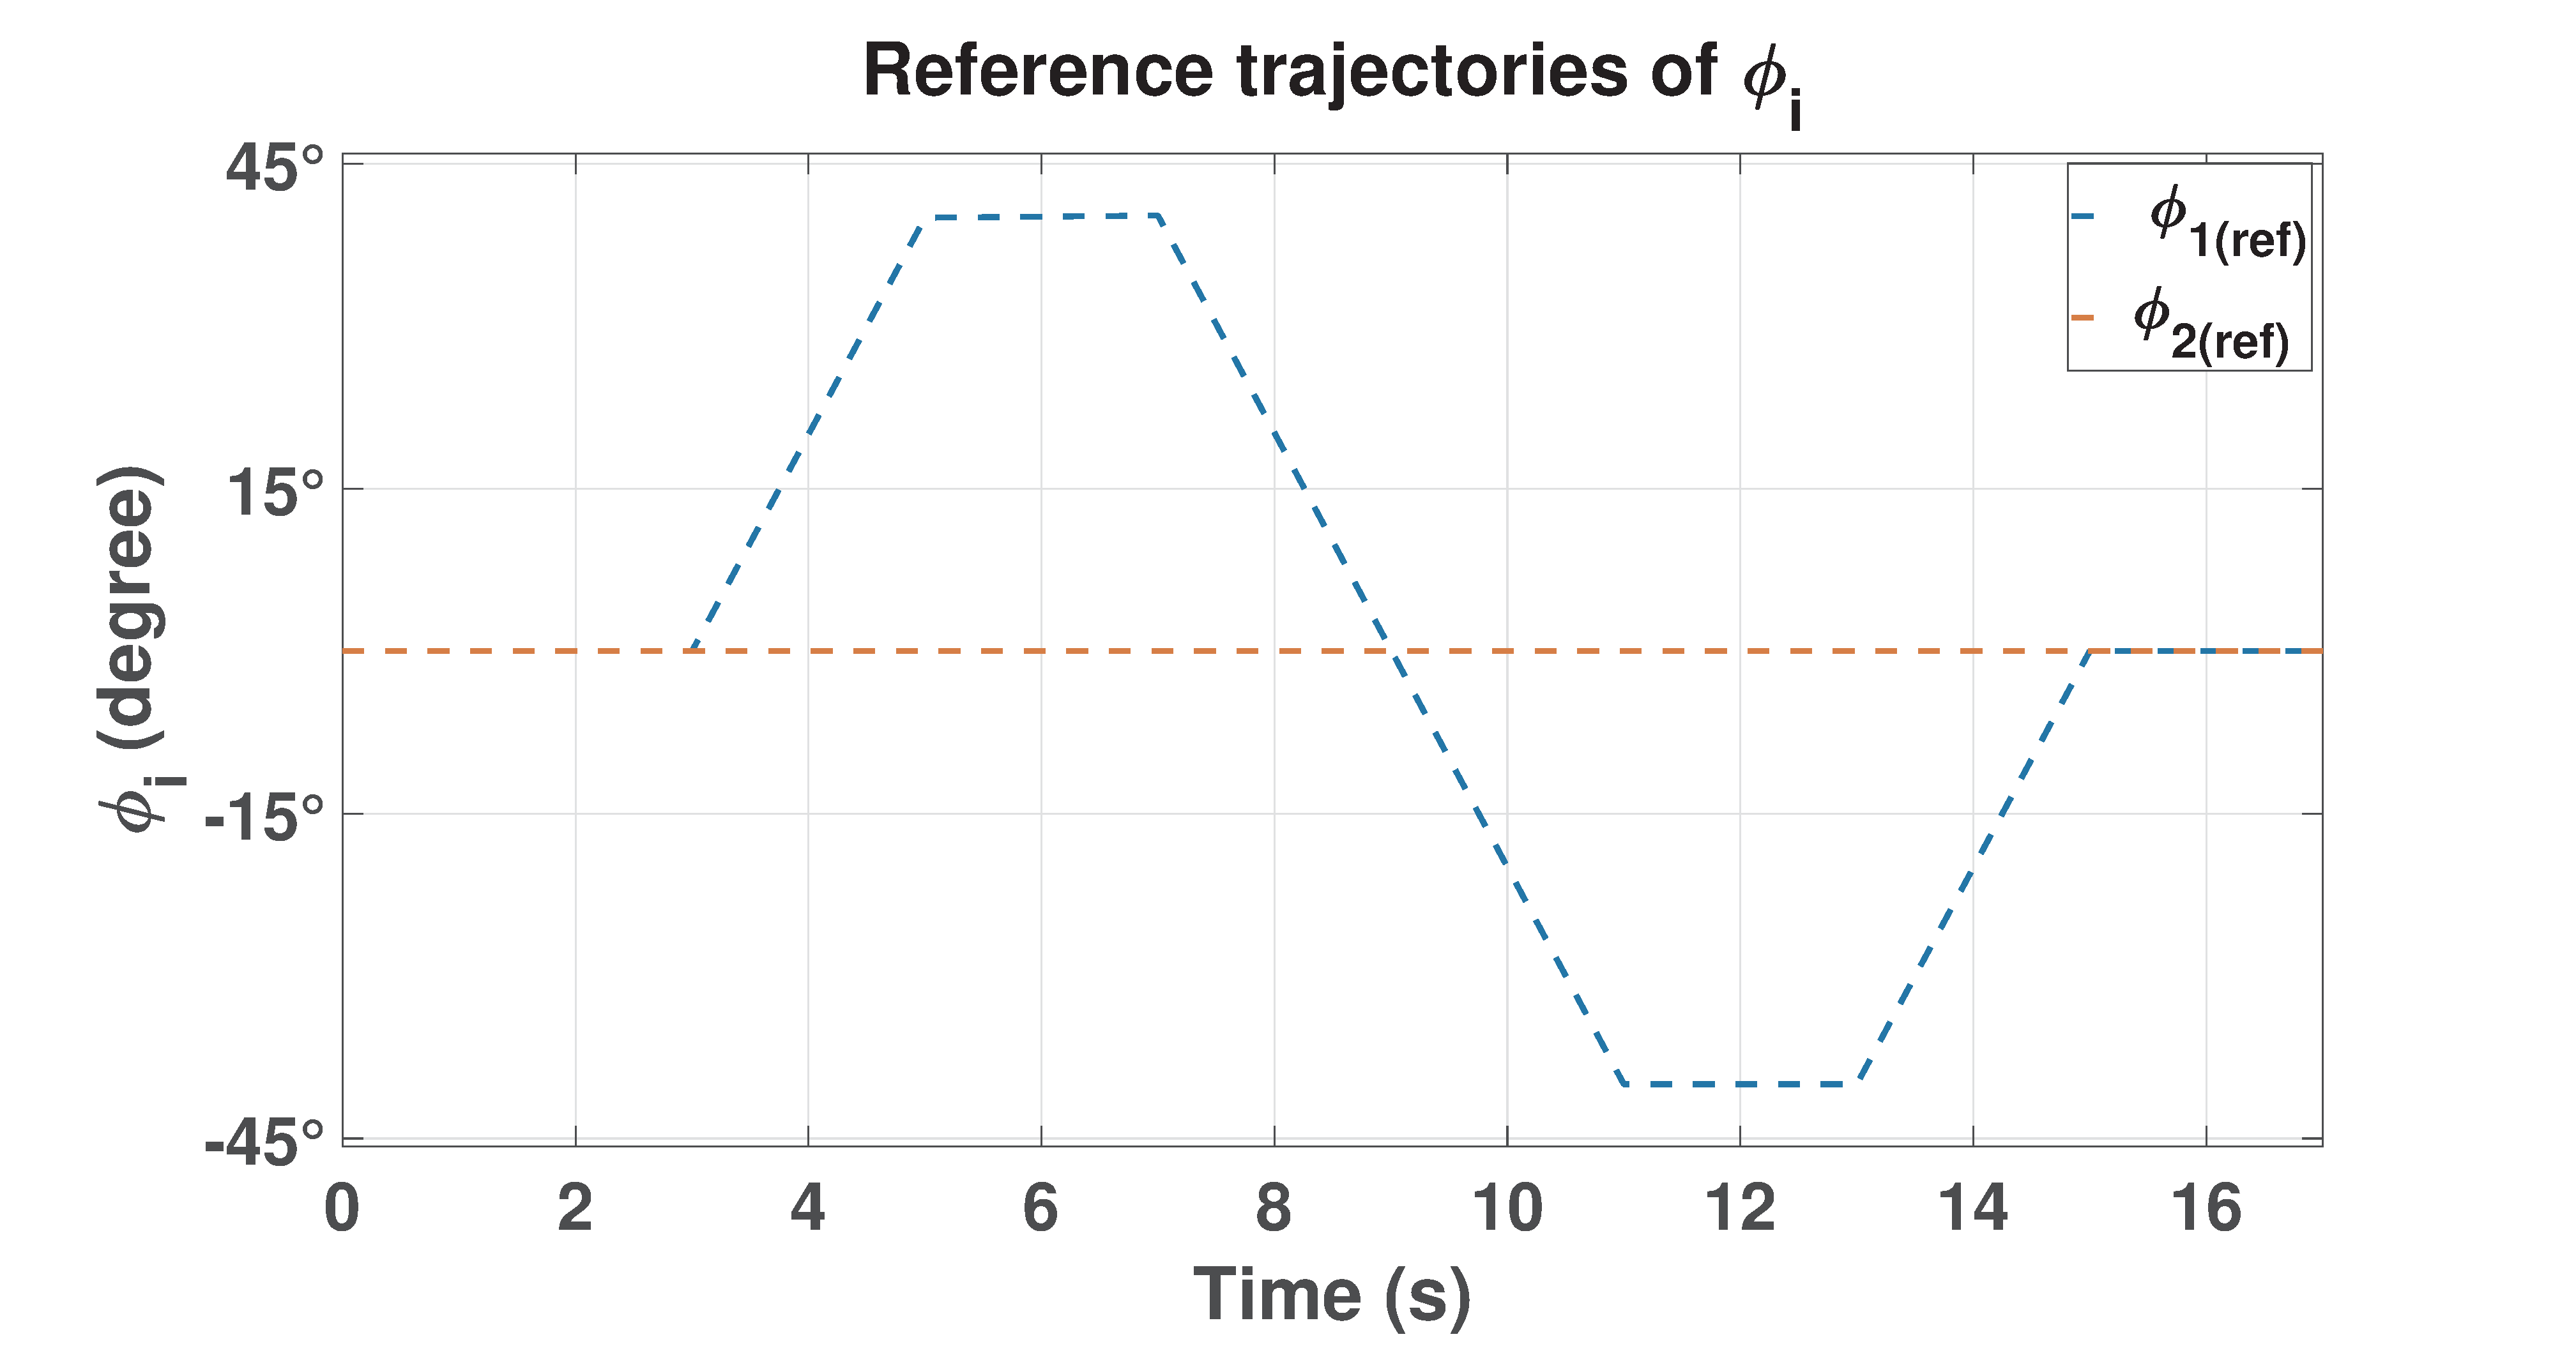
\includegraphics[width=1\linewidth]{figures/Reference}
    \caption{Reference trajectory of the states ($\phi_1$ and $\phi_2$).}
    \label{fig:ReferenceTraj}
    \end{subfigure}%
    \vspace{0.5em}
    \begin{subfigure}[t]{0.485\textwidth}
    \centering
    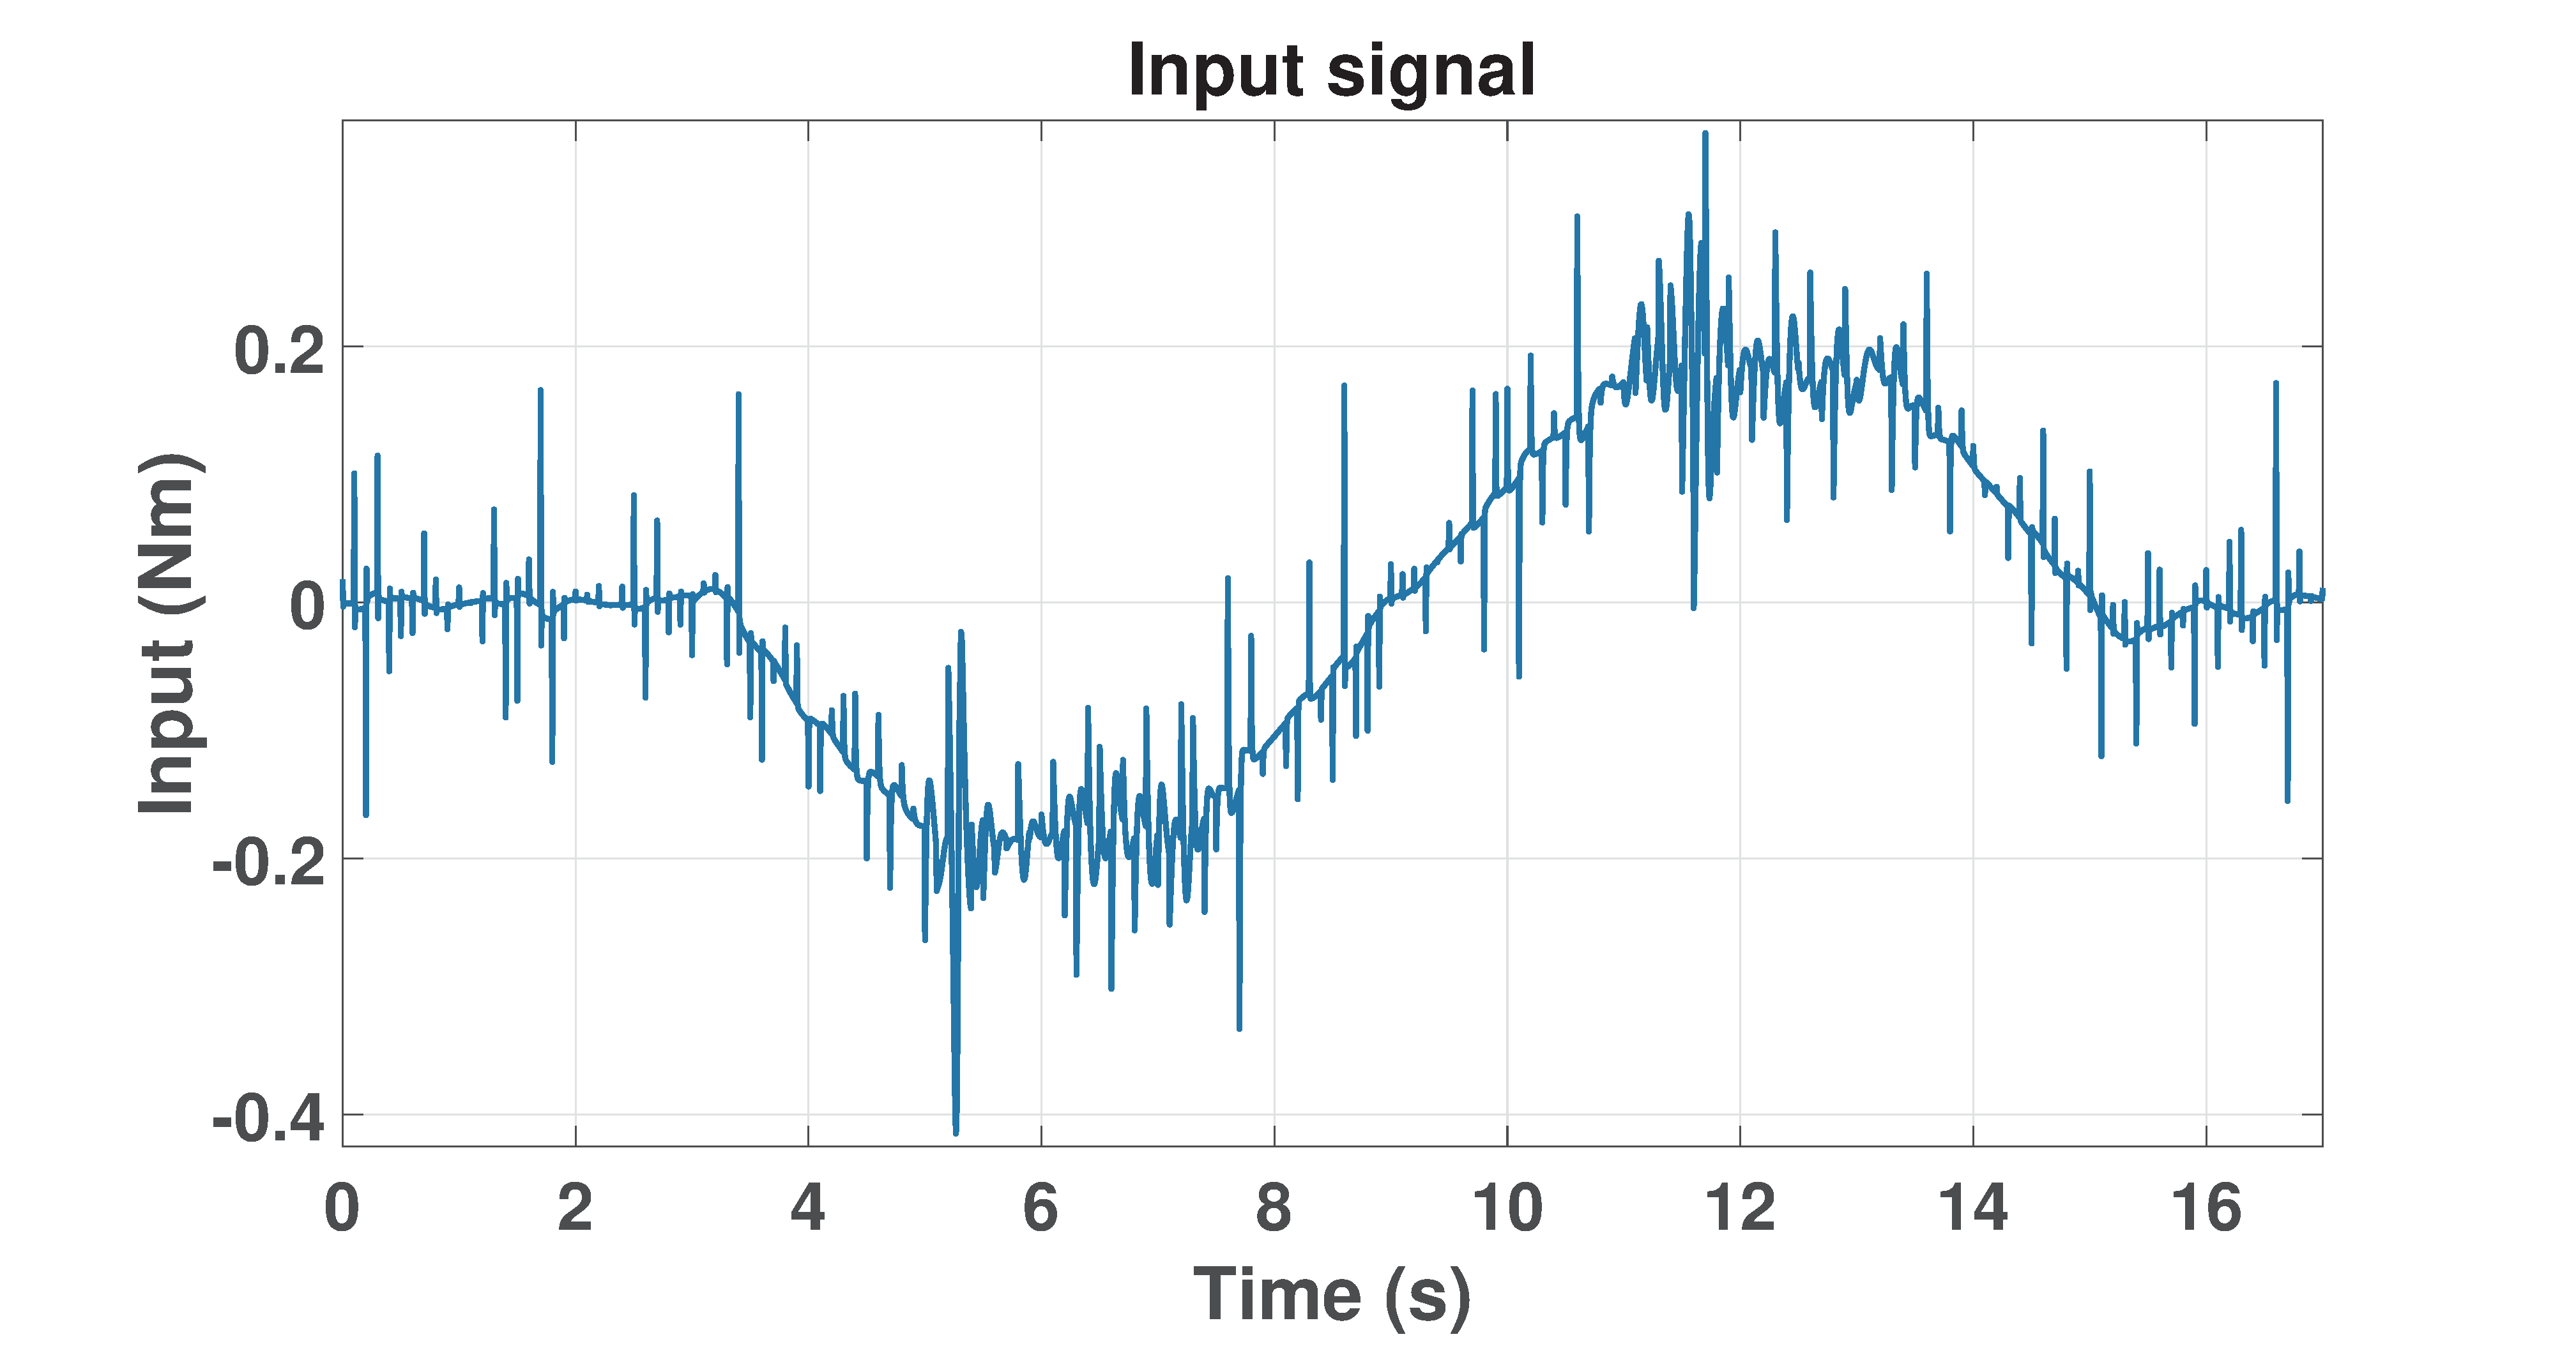
\includegraphics[width=\textwidth]{figures/RefInput}
    \caption{Input signal}
    \label{fig:InputSignal}
    \end{subfigure}
    ~
    \begin{subfigure}[t]{0.485\textwidth}
    \centering
    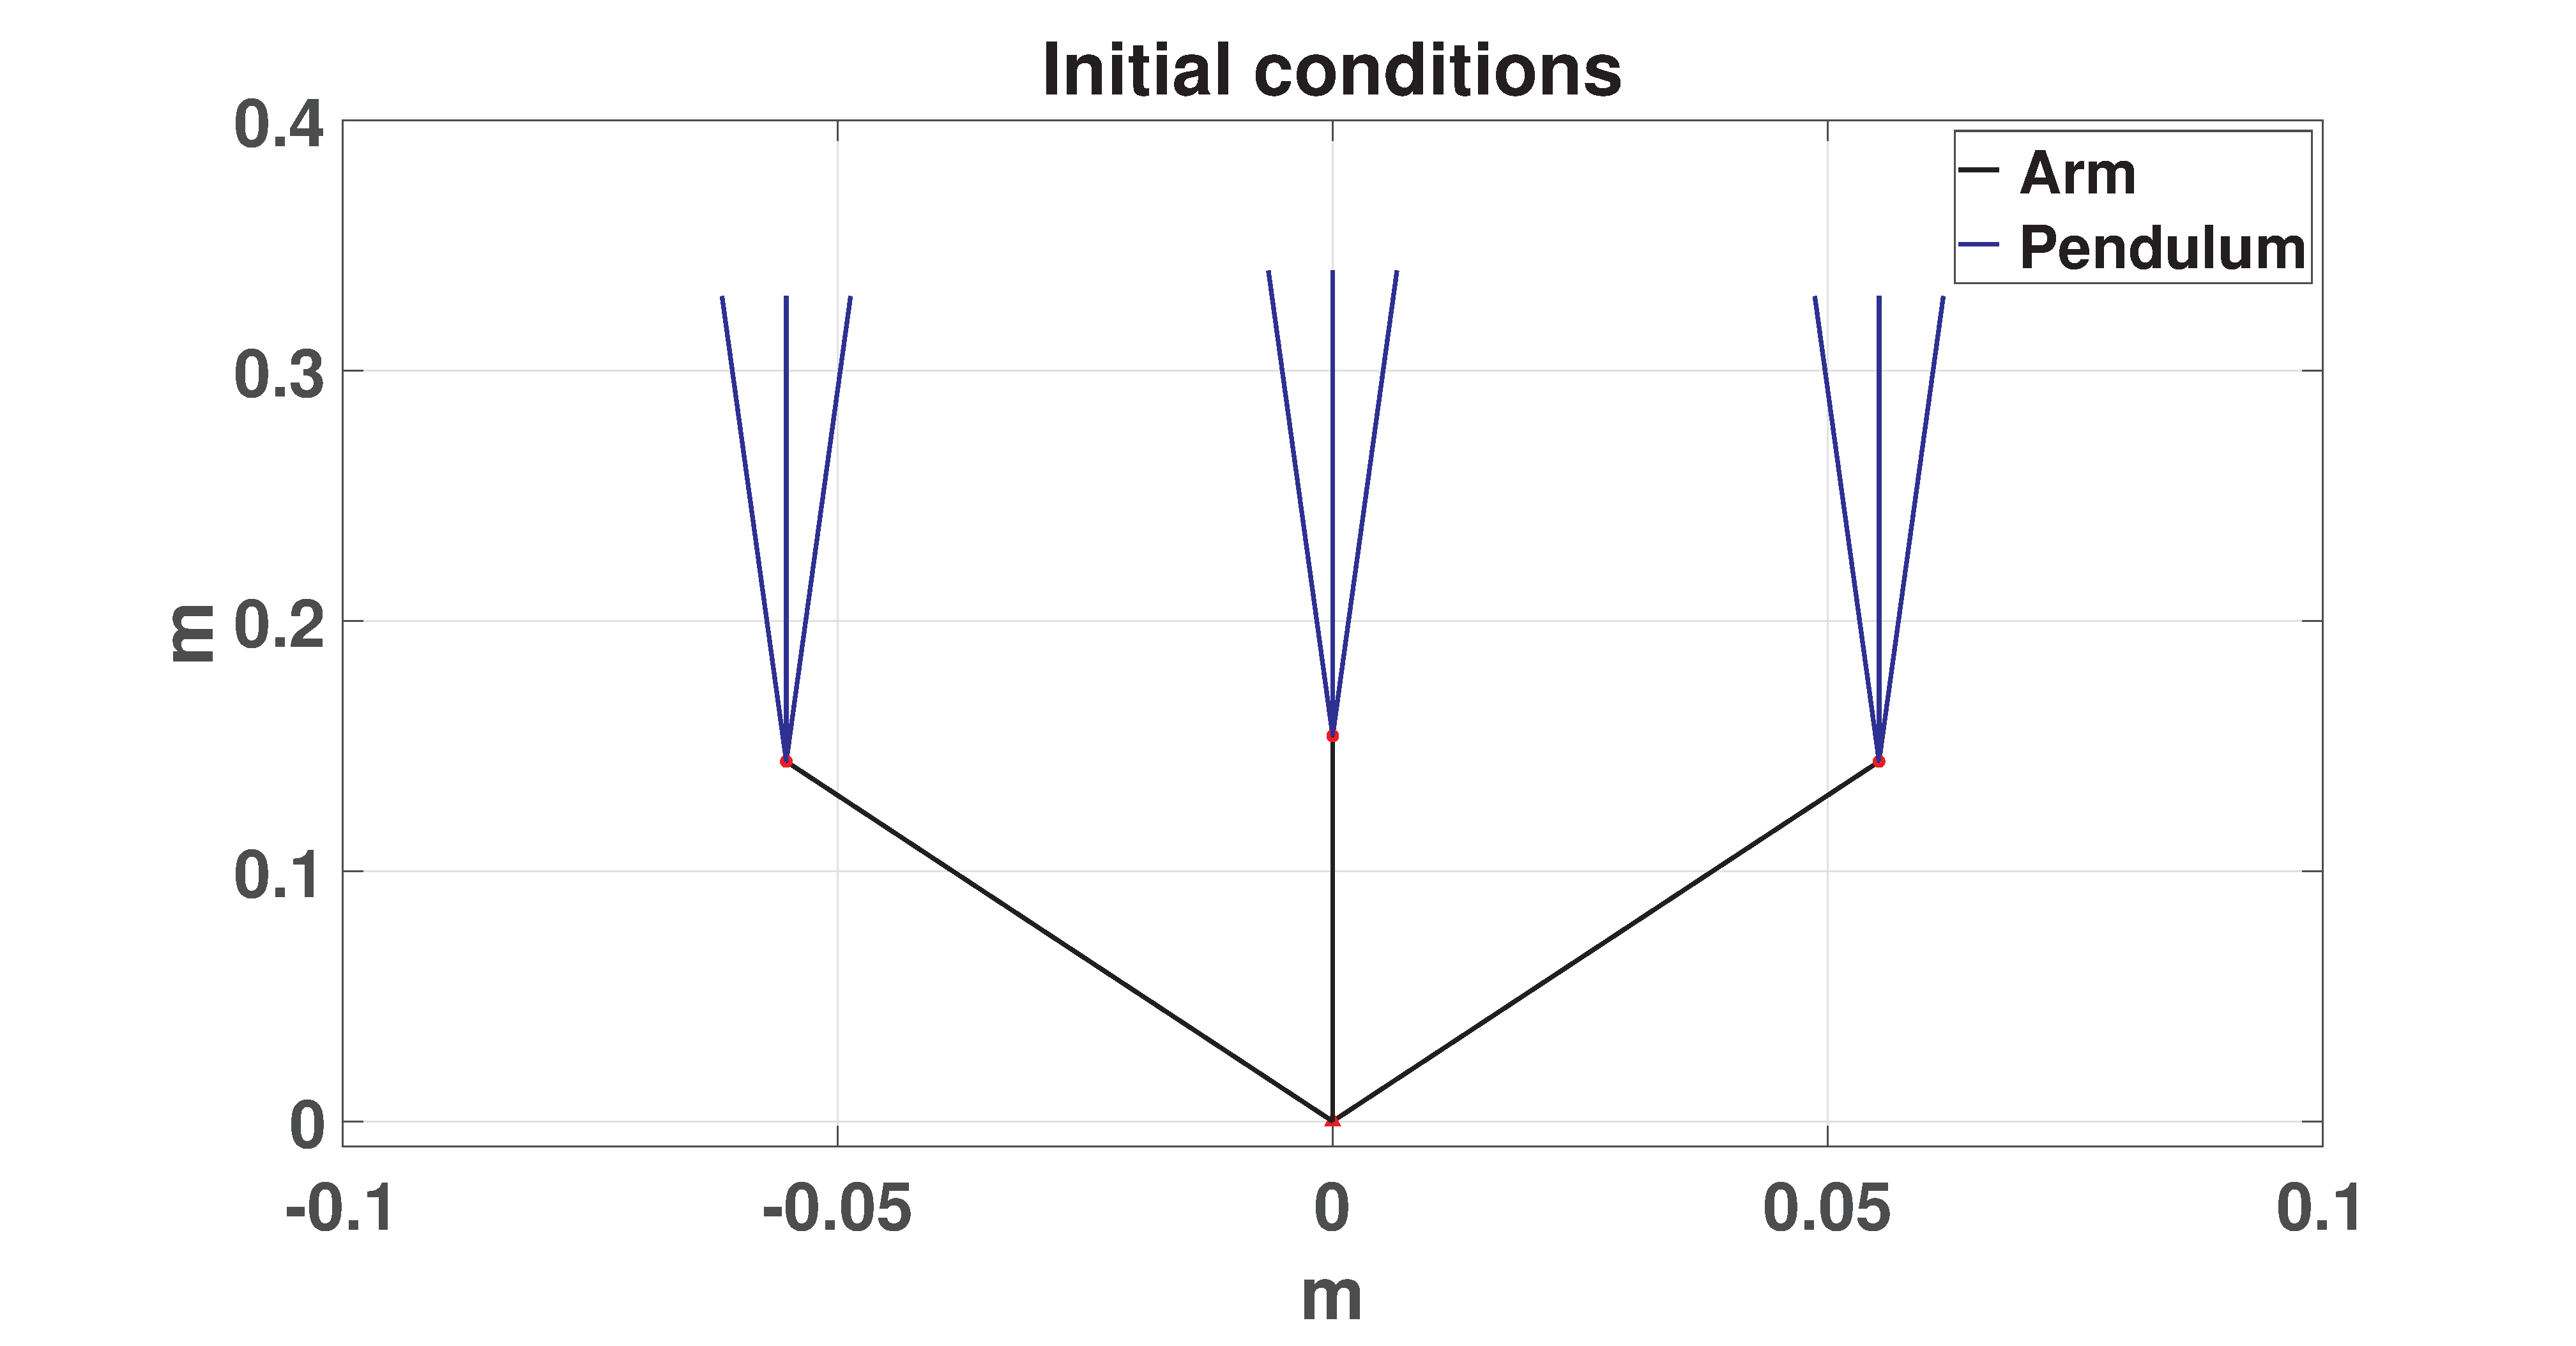
\includegraphics[width=\textwidth]{figures/InitCondn}
    \caption{Visualization of the initial conditions}
    \label{fig:InitCondns}
    \end{subfigure}
    \caption{Reference trajectory, Input signal and Initial conditions}
\end{figure}
\newpage
Data was collected by simulating the system multiple times in closed-loop with random initial conditions given by
\begin{equation}
\label{Eq:MultInit}
    \mathbf{x}_0 = [\mathcal{U}(-1 \quad 1)l_{\phi_1},~\mathcal{U}(-1 \quad 1)l_{\phi_2},~\mathcal{U}(-1 \quad 1)l_{\dot{\phi}_1},~\mathcal{U}(-1 \quad 1)l_{\dot{\phi}_2}] \;,
\end{equation}
where~ $\mathcal{U}(-1,~1)$ is a uniformly distributed random variable with range $-1$ to $1$, and $l_{\phi_1} = 40^{\circ}$, $l_{\phi_2} = 2^{\circ}$, $l_{\dot{\phi}_1} = l_{\dot{\phi}_2} = 0.25$rad/s. Therefore, the initial condition is uniformly distributed around the unstable equilibrium ($\phi_1 = \phi_2 = \dot{\phi}_1 = \dot{\phi}_2 = 0^{\circ}$) and its range is defined by $L = [l_{\phi_1}, l_{\phi_2}, l_{\dot{\phi}_1}, l_{\dot{\phi}_2} ]$. Figure \ref{fig:InitCondns} visualizes the distribution of initial conditions with respect to the states $\phi_1$ and $\phi_2$. $L$ was chosen by trial-and-error and it represents the range limit in which the controller is able to track the subsequent reference trajectory successfully. One might also choose $L$ by evaluating a regulation task instead of tracking. The data was generated by simulations of 17s each on a nonlinear model of the ADIP (refer Chapter \ref{Chapter:Plant}) where the controller tracked the reference trajectory~(Fig.~\ref{fig:ReferenceTraj}). The data was sampled every 5ms. The subsequent approximation of the linear matrices follows the procedure detailed in Section \ref{sec:EDMD}. \par
As stated previously, although the region of interest for this thesis work is the up-up configuration for which only closed-loop identification is possible, open-loop identification around the stable equilibrium nevertheless presents numerous important insights into the generation of data and choice of observables, which was then applied to generate data and/or influenced the choice of observables in closed-loop identification. During the course of this thesis, numerous combinations of observables and data were tried and analyzed, and this could not have been easily done in the up-up configuration as it demands a corresponding controller to stabilize the system.\par
In this thesis, SINDy with control (SINDYc) algorithm (refer Section \ref{sec:SINDy}) is used to approximate the open-loop dynamics to demonstrate the working of SINDy algorithm. EDMDc can also very well be used for the same. However, SINDYc approximates the states' time evolution directly from data and a set of candidate functions without having to go through the hassle of choosing the `correct' observables and computing the corresponding Koopman operator. It is important to note that SINDYc has also been used for feedback control of nonlinear systems \cite{SINDyc}; however, this has not been implemented in this work.\par
The forcing function used in open-loop identification is a chirp signal with the frequency defined in the range $[f_{min}~ f_{max}]$ and with amplitude $A$. The frequencies and amplitudes were chosen such that the system does not translate to the `chaotic zone' but is also sufficiently perturbed away from its stable equilibrium. The chirp signal can be generated using the \textit{chirp} command in Matlab. In summary, the forcing functions for training and validation purposes are given as,
% 
\begin{align}
\label{Eq:Forcing}
\begin{split}
    \textup{Training} &\rightarrow A*chirp(t,f_{min},t_s,f_{max},[~],-90), \quad [f_{min}~f_{max}] = [0.3 ~ 0.7]\textup{Hz}, A = 0.1 \;, \\ 
    \textup{Validation} &\rightarrow A*chirp(t,f_{min},t_s,f_{max},[~],-90), \quad [f_{min}~f_{max}] = [0.7 ~ 0.9]\textup{Hz}, A = 0.065 \;.
\end{split}
\end{align}
% 
First, the case for data obtained from multiple trajectories is made. As Abraham et al. \cite{Abraham} observed, the number of data points and their distribution across the state space will have a large effect on the computed Koopman operator of the underlying nonlinear system. It is always beneficial to record trajectories from multiple initial conditions as shown in (\ref{Eq:MultInit}).\par
Figures \ref{fig:SingleTrajTrain} and \ref{fig: MultTrajTrain} compare the identification of the system through SINDYc from training data generated by a single initial condition and training data generated from multiple initial conditions respectively. The training data generated from multiple initial conditions is visualized in Figure \ref{fig:TrainingData}. In this case, the training data is generated from multiple initial conditions (\ref{Eq:MultInit}) with $l_{\phi_1} = 210^{\circ}$, $l_{\phi_2} = 150^{\circ}$, $l_{\dot{\phi}_1} = l_{\dot{\phi}_2} = 1$rad/s and the forcing function~(\ref{Eq:Forcing}) with $f_{min} = f_{max} = 0.5$Hz and $A = 0.1$, respectively. Again, the choice of these values are influenced by the requirement for trajectories to lie in the non-chaotic zone.
\begin{figure}[ht]
    \centering
    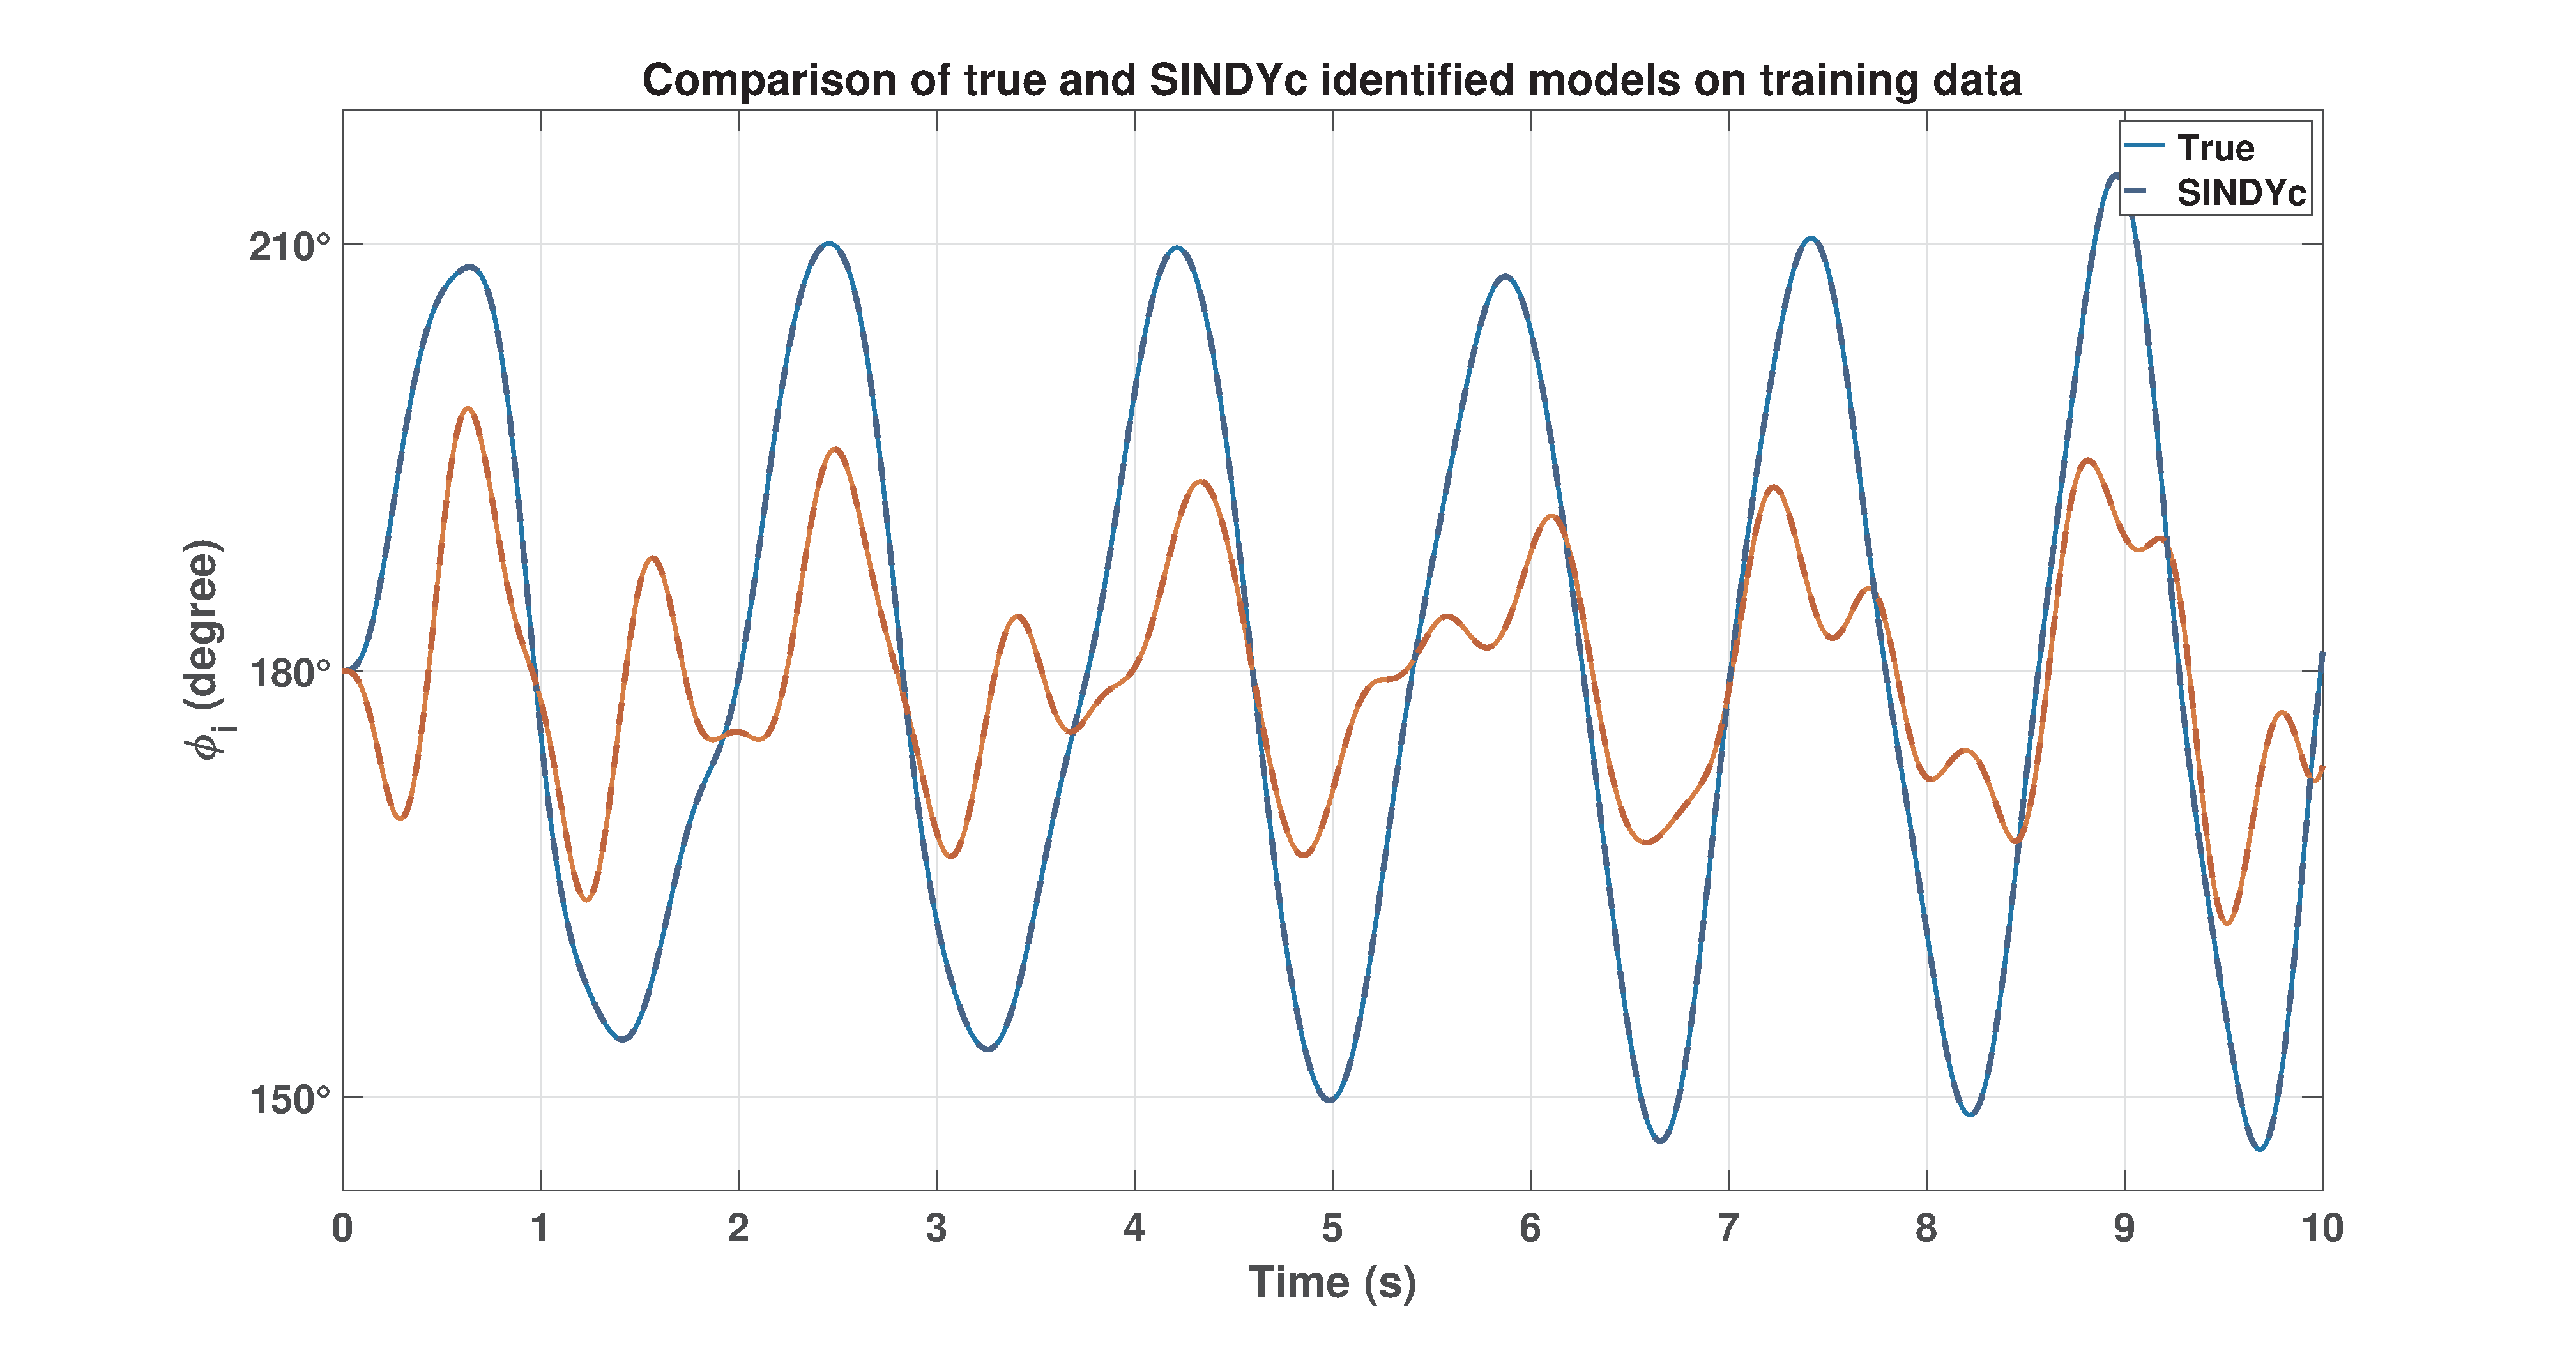
\includegraphics[width=0.915\linewidth]{figures/SingleTrajTrain_2_0_1}
    \caption{Identification with single trajectory and $\mathbf{\Psi_3}$ on training data. (\textcolor{blue}{\textbf{--}}) and (\textcolor{red}{\textbf{--}}) represent the trajectories of $\phi_1$ and $\phi_2$, respectively}
\label{fig:SingleTrajTrain}
\end{figure}
\vspace{0em}
\begin{figure}[ht]
    \centering
    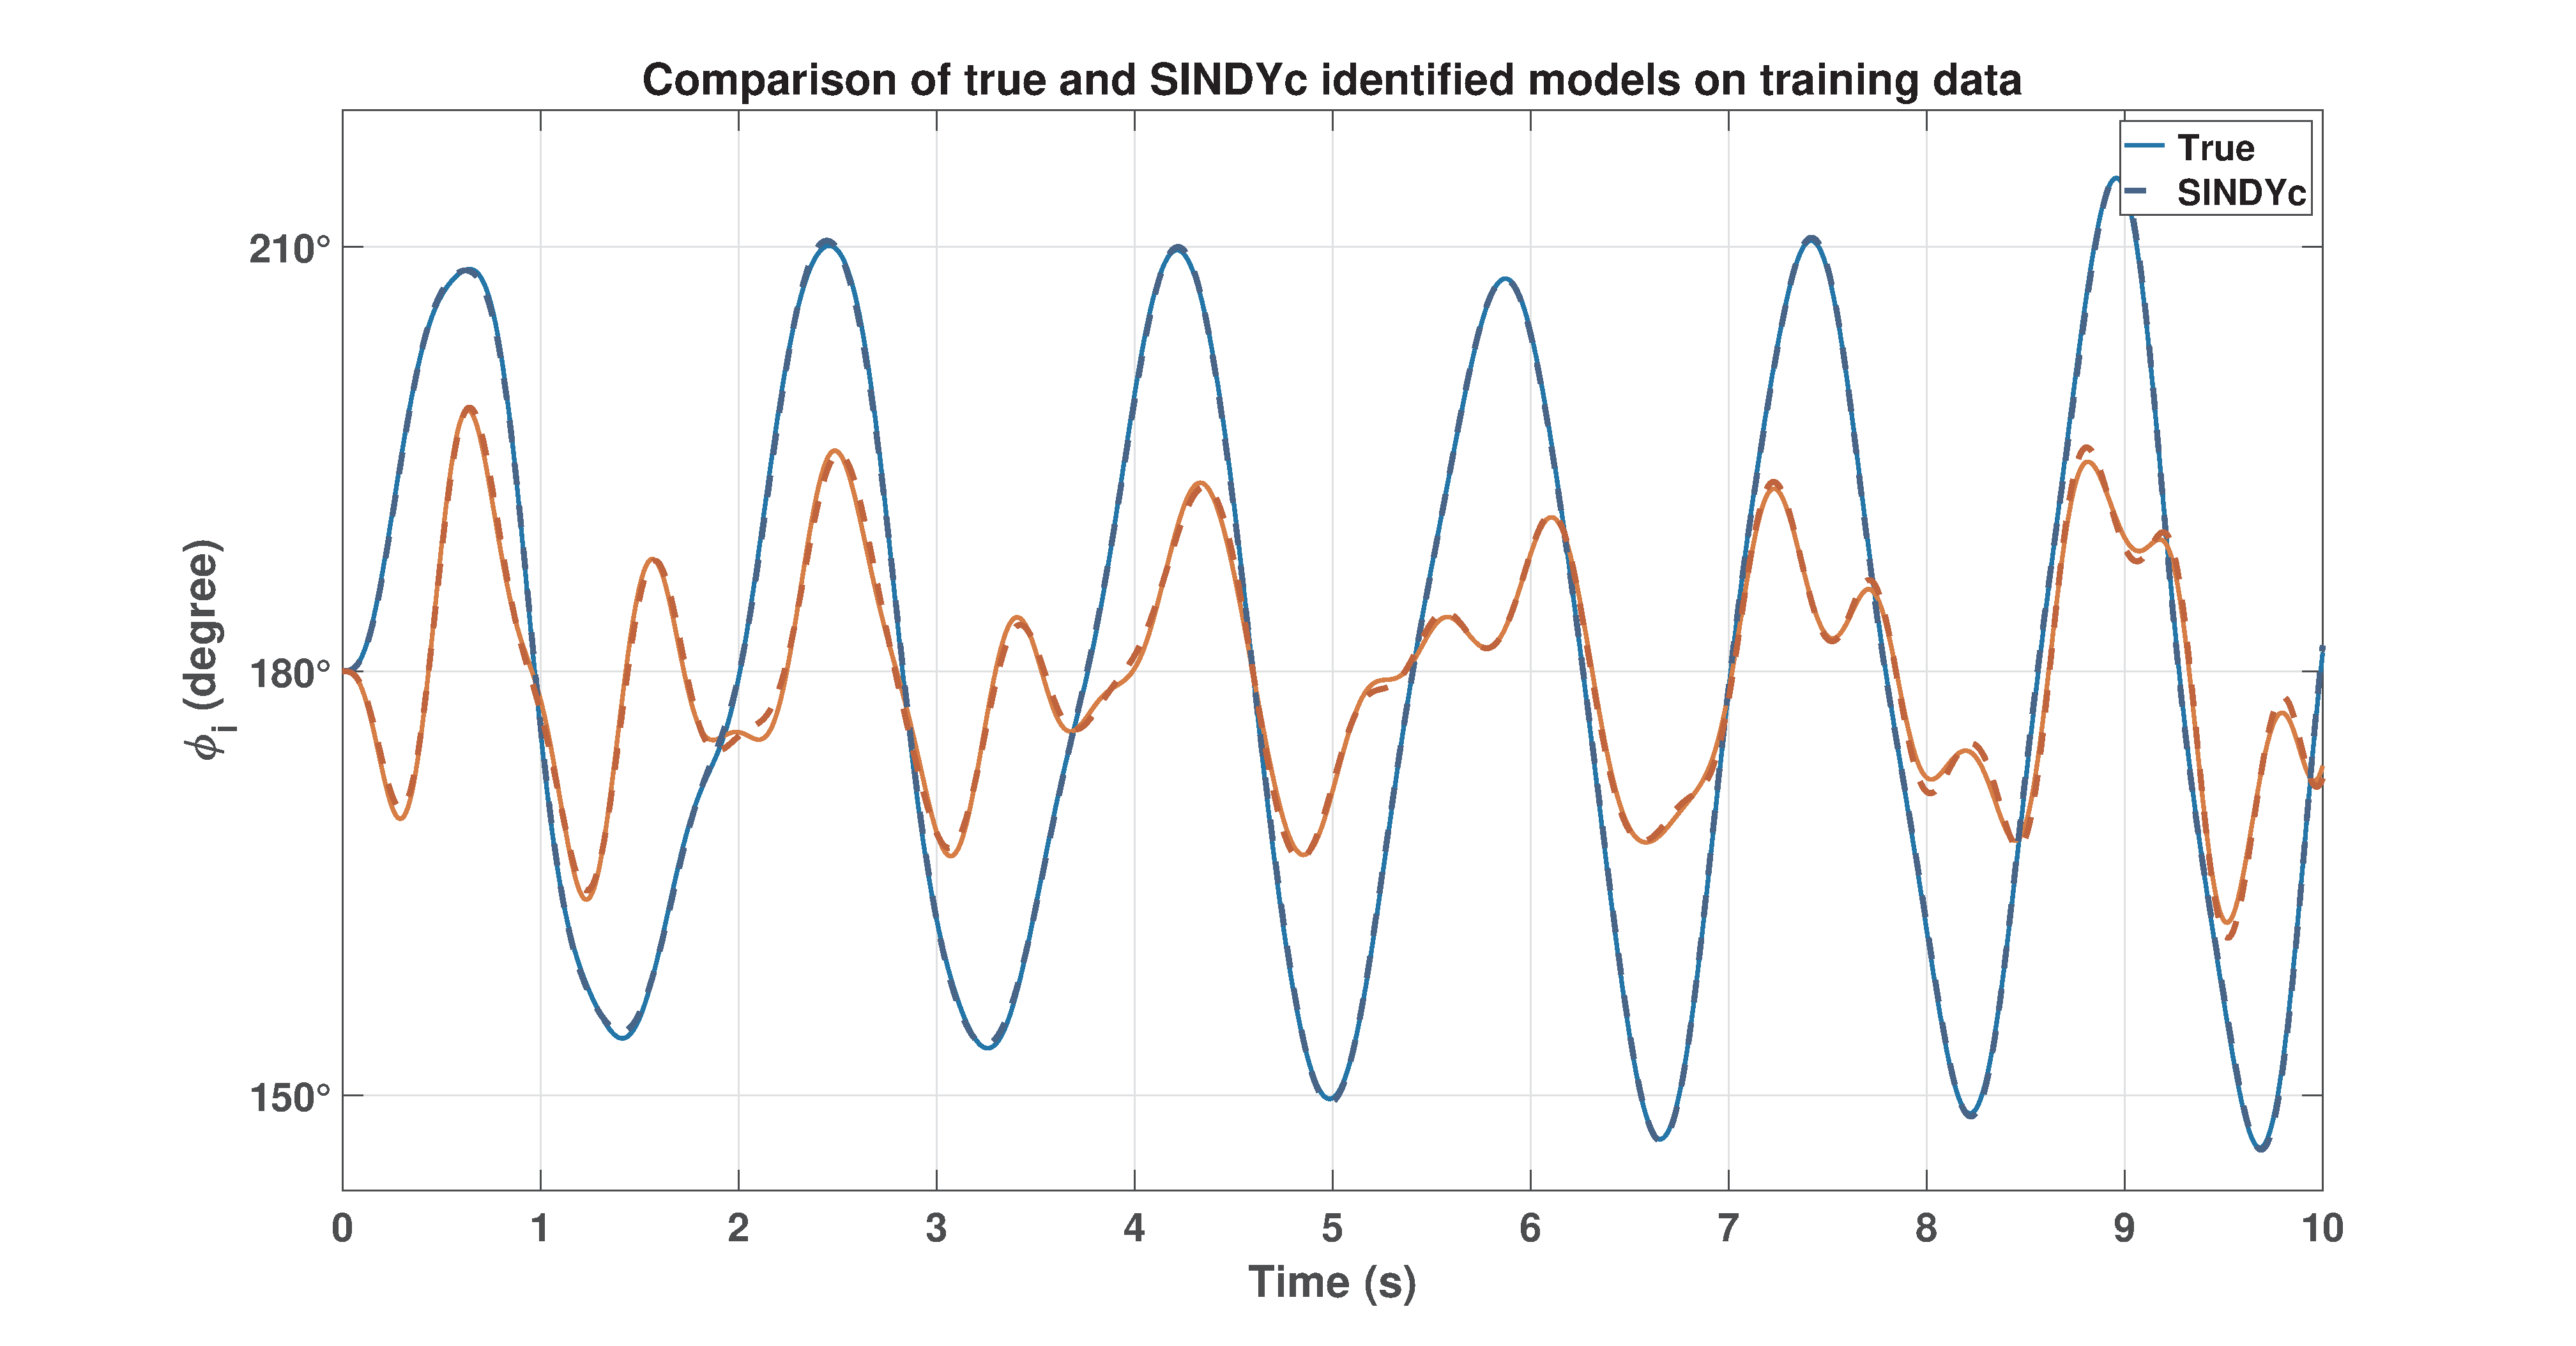
\includegraphics[width=0.915\linewidth]{figures/MultTrajtrain_2_0_1}
    \caption{Identification with multiple trajectories and $\mathbf{\Psi_3}$ on training data.}
    \label{fig: MultTrajTrain}
\end{figure}
% 
% 
\begin{figure}[ht]
    \centering
    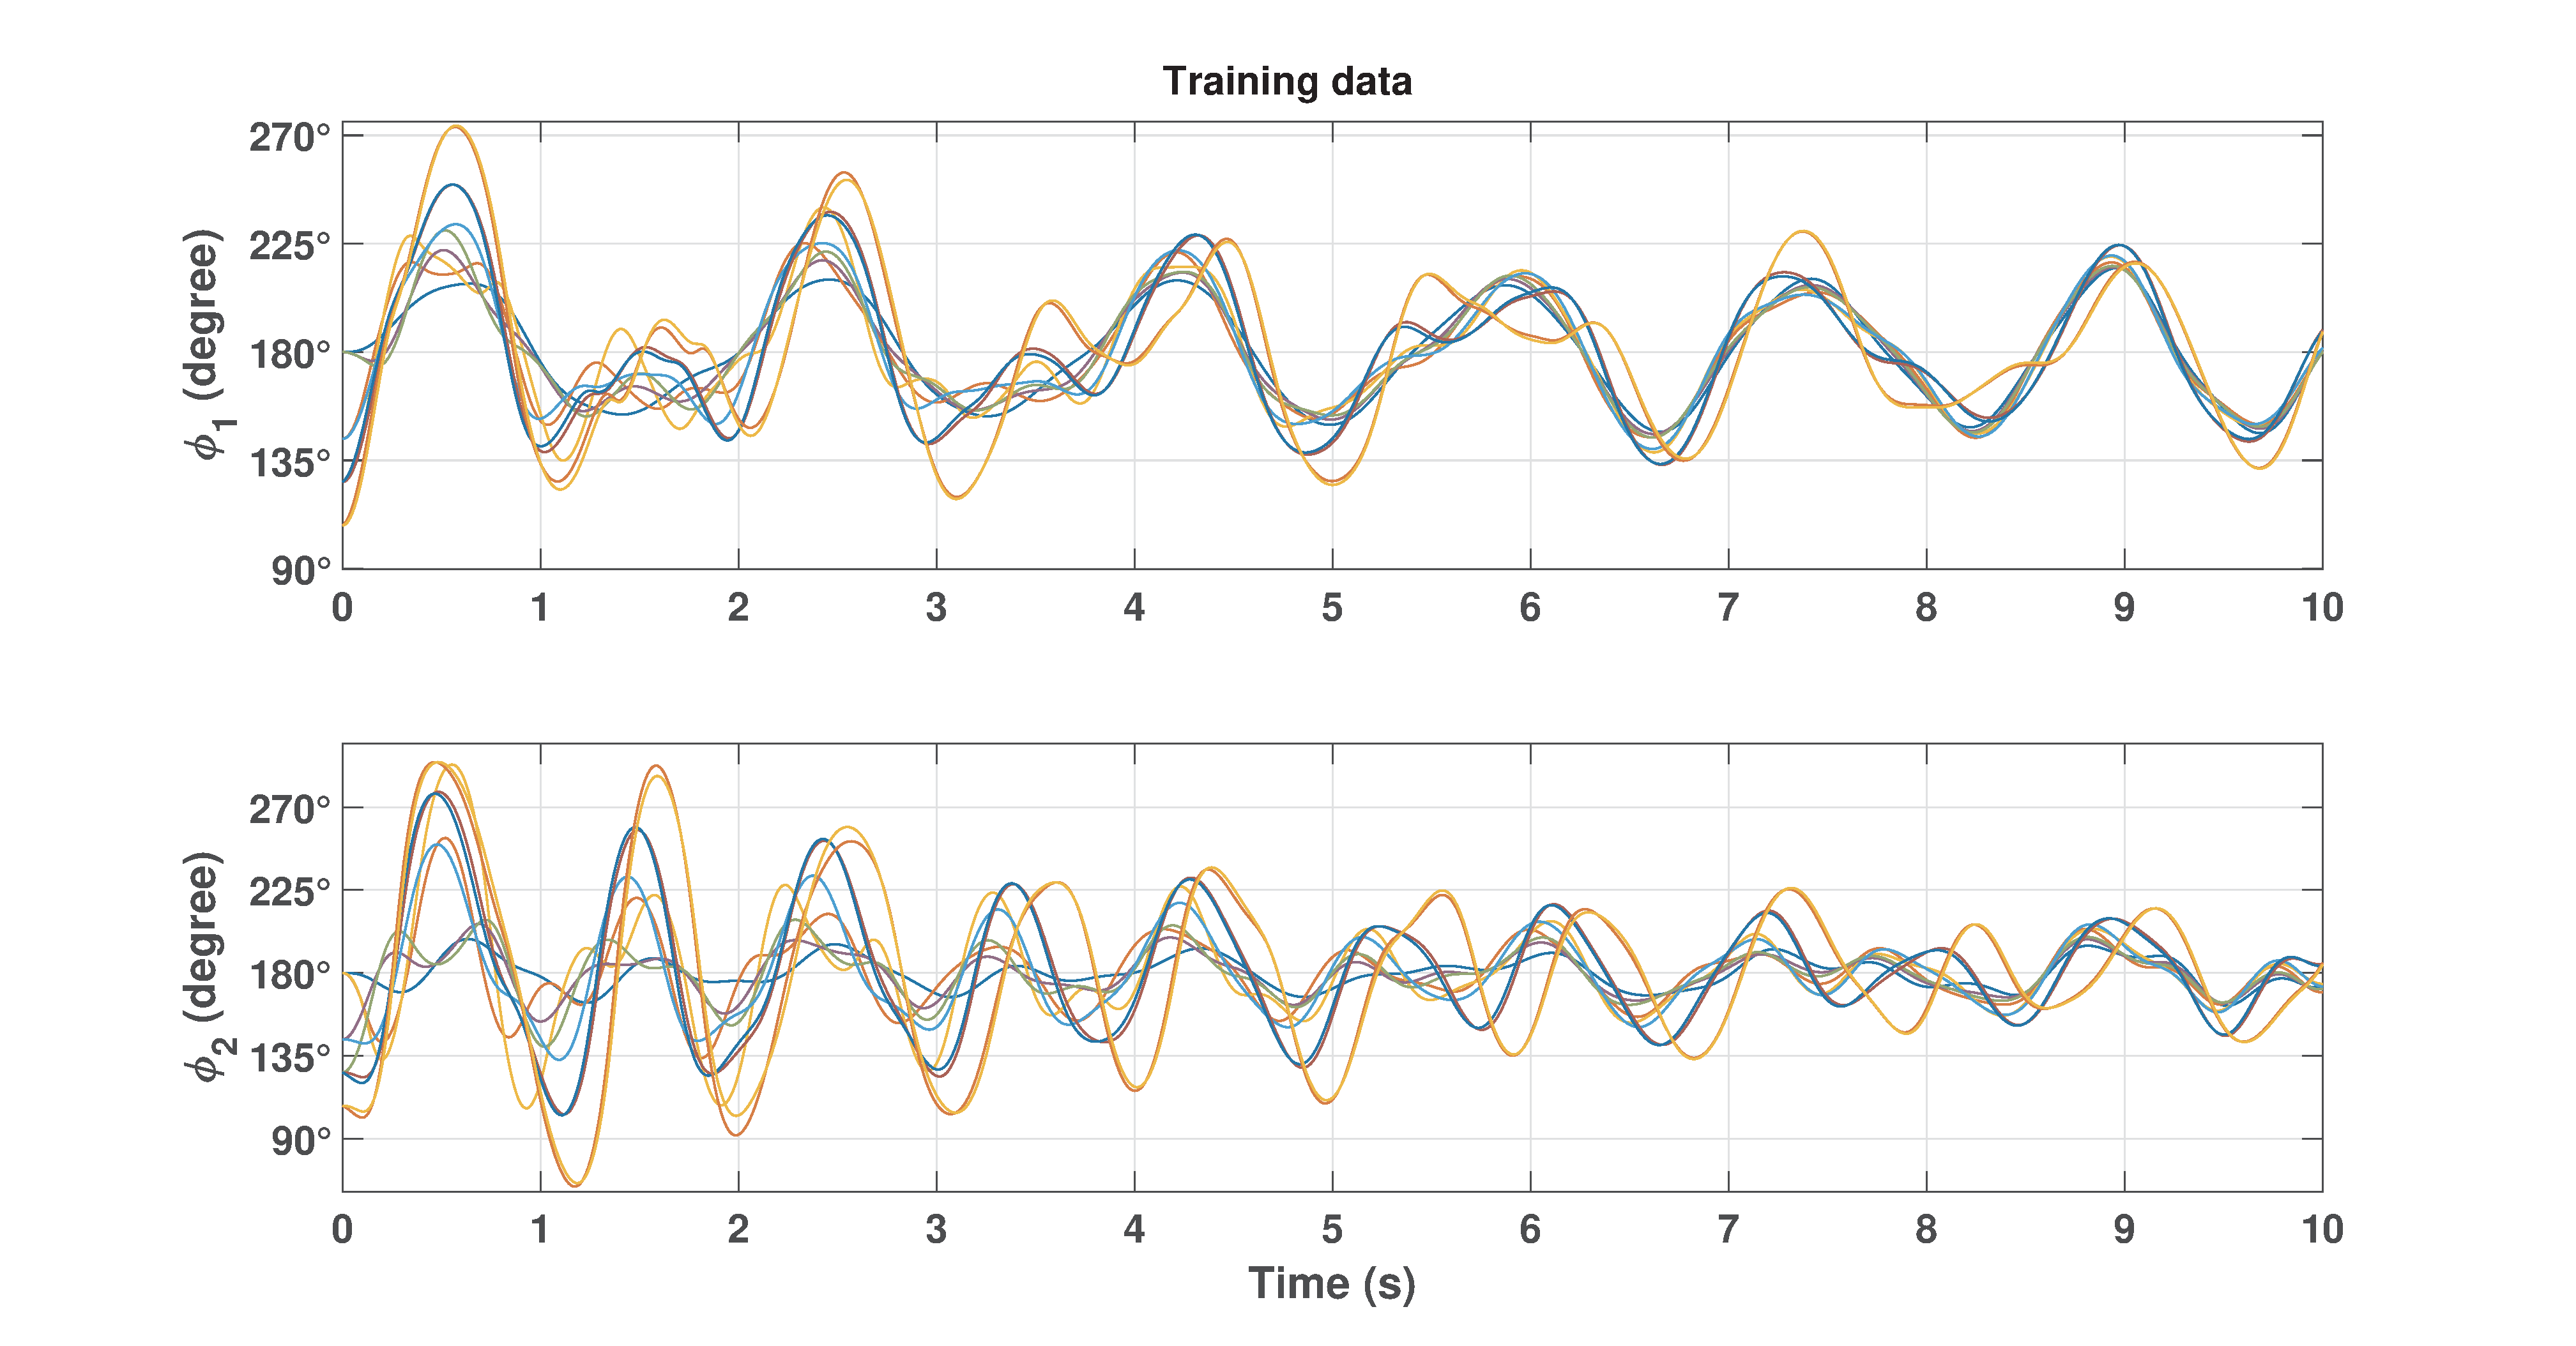
\includegraphics[width=1\linewidth]{figures/TrainingData}
    \caption{Training data from multiple trajectories}
    \label{fig:TrainingData}
\end{figure}
\newpage
In the above figures, $\mathbf{\Psi_3}$ is a vector of observables that is already defined in Section \ref{Chapter:Data}. From the above figures, one can see that the SINDYc algorithm almost perfectly identifies the time evolution of the state trajectories both in the case of training data obtained from a single initial condition and multiple initial conditions for a specific choice of candidate functions.\par
Even though it might seem that data from a single trajectory is enough to approximate the dynamics, this will almost always fail when the system is forced with a forcing function that is different from the forcing function used to generate the training data. Revisiting Section \ref{sec:SINDy}, SINDY-with-control~(SINDYc) computes a (tall) sparse matrix of coefficients of the candidate functions $\mathbf{\Xi}$ (which also contains the input function), and this matrix of coefficients is then used to simulate the dynamics for a new forcing function. Figures \ref{fig:SingleTrajVal} and \ref{fig: MultTrajVal} show the prediction of dynamics evaluated on the matrix of coefficients generated from training data for a new `validation' forcing function in (\ref{Eq:Forcing}). It is interesting to note that while the $\mathbf{\Xi}$ generated from a single trajectory worked perfectly well for data that lies within the range of training data, it fails to correlate the dynamics over a longer time span when the forcing function drives the trajectory away from the training trajectory, as observed in Fig \ref{fig:SingleTrajVal}. The predicted trajectory by SINDYc fails to follow the reference trajectory after approximately 1.5 seconds, where both the amplitude and the frequency of the reference trajectory differ from the trajectory used for training. Whereas, in Fig.~\ref{fig: MultTrajVal} it is seen that the dynamics are approximately predicted for $\mathbf{\Xi}$ generated from multiple trajectories for a `good' choice of observables. Therefore, it is vital to generate data from multiple trajectories and train the regressors, be it SINDYc or EDMDc, for a close approximation of the dynamics. 
% 
\begin{figure}[ht]
    \centering
    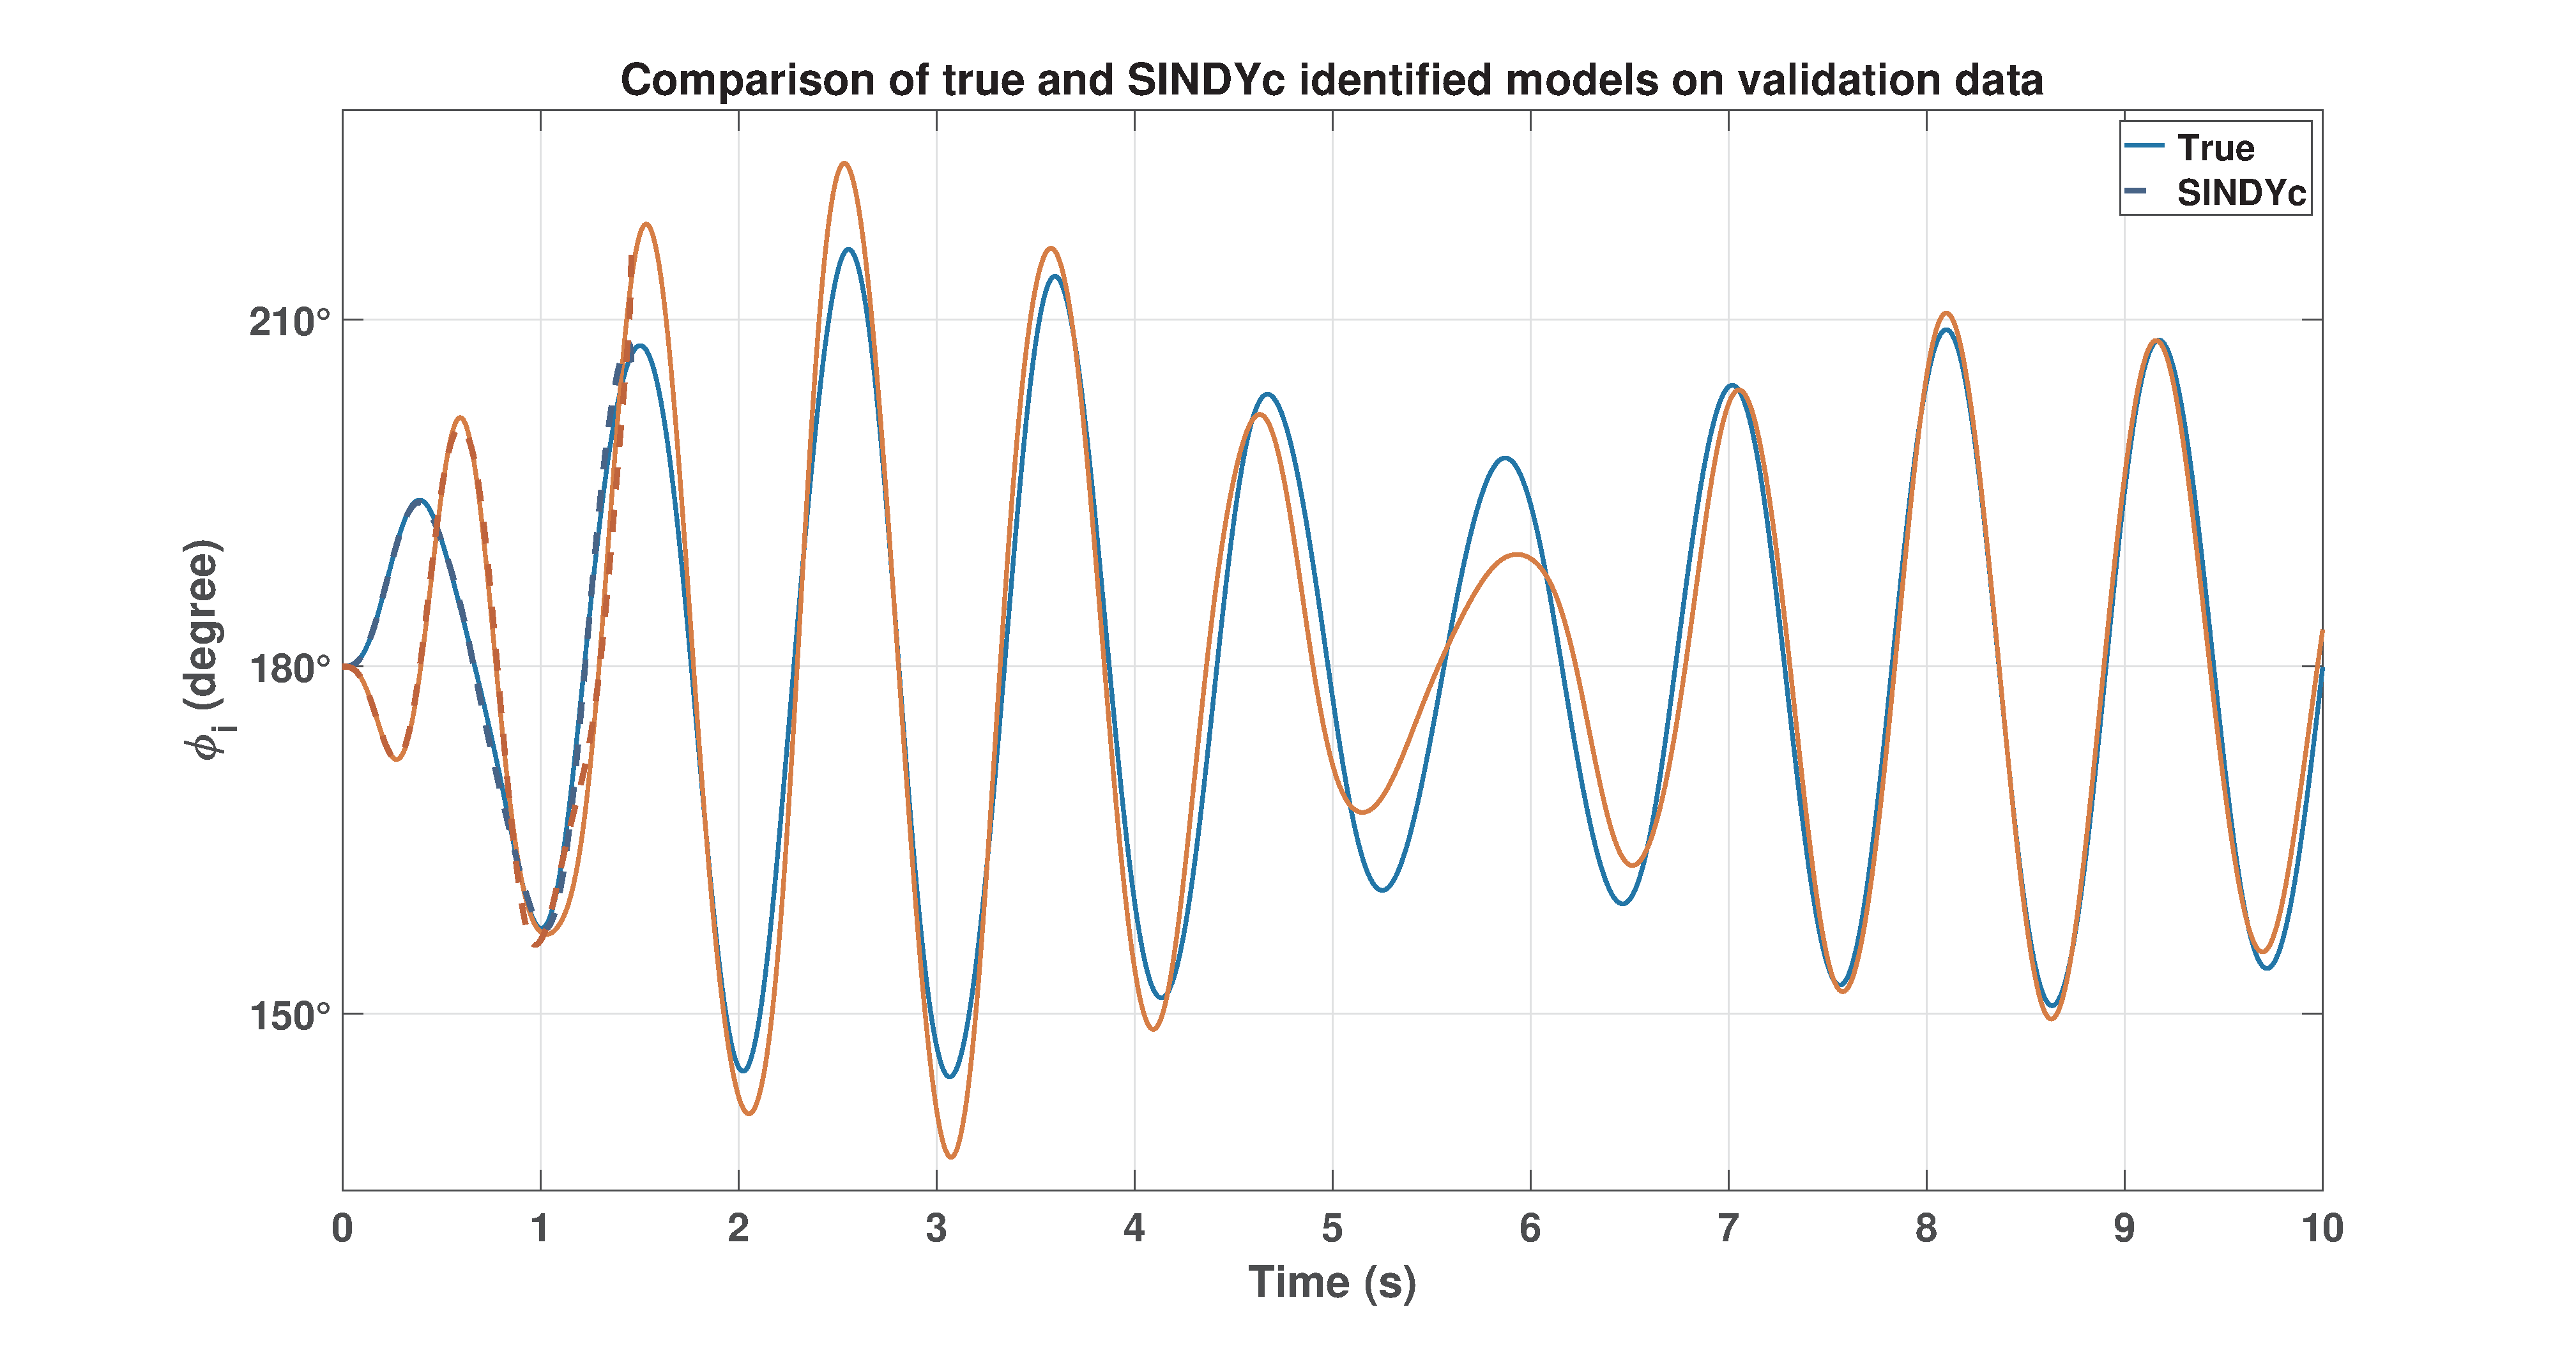
\includegraphics[width=1\linewidth]{figures/SingleTrajVal_2_0_1}
    \caption{Identification with single trajectory and $\mathbf{\Psi_3}$ on validation data}
    \label{fig:SingleTrajVal}
\end{figure}
% 
\begin{figure}[ht]
    \centering
    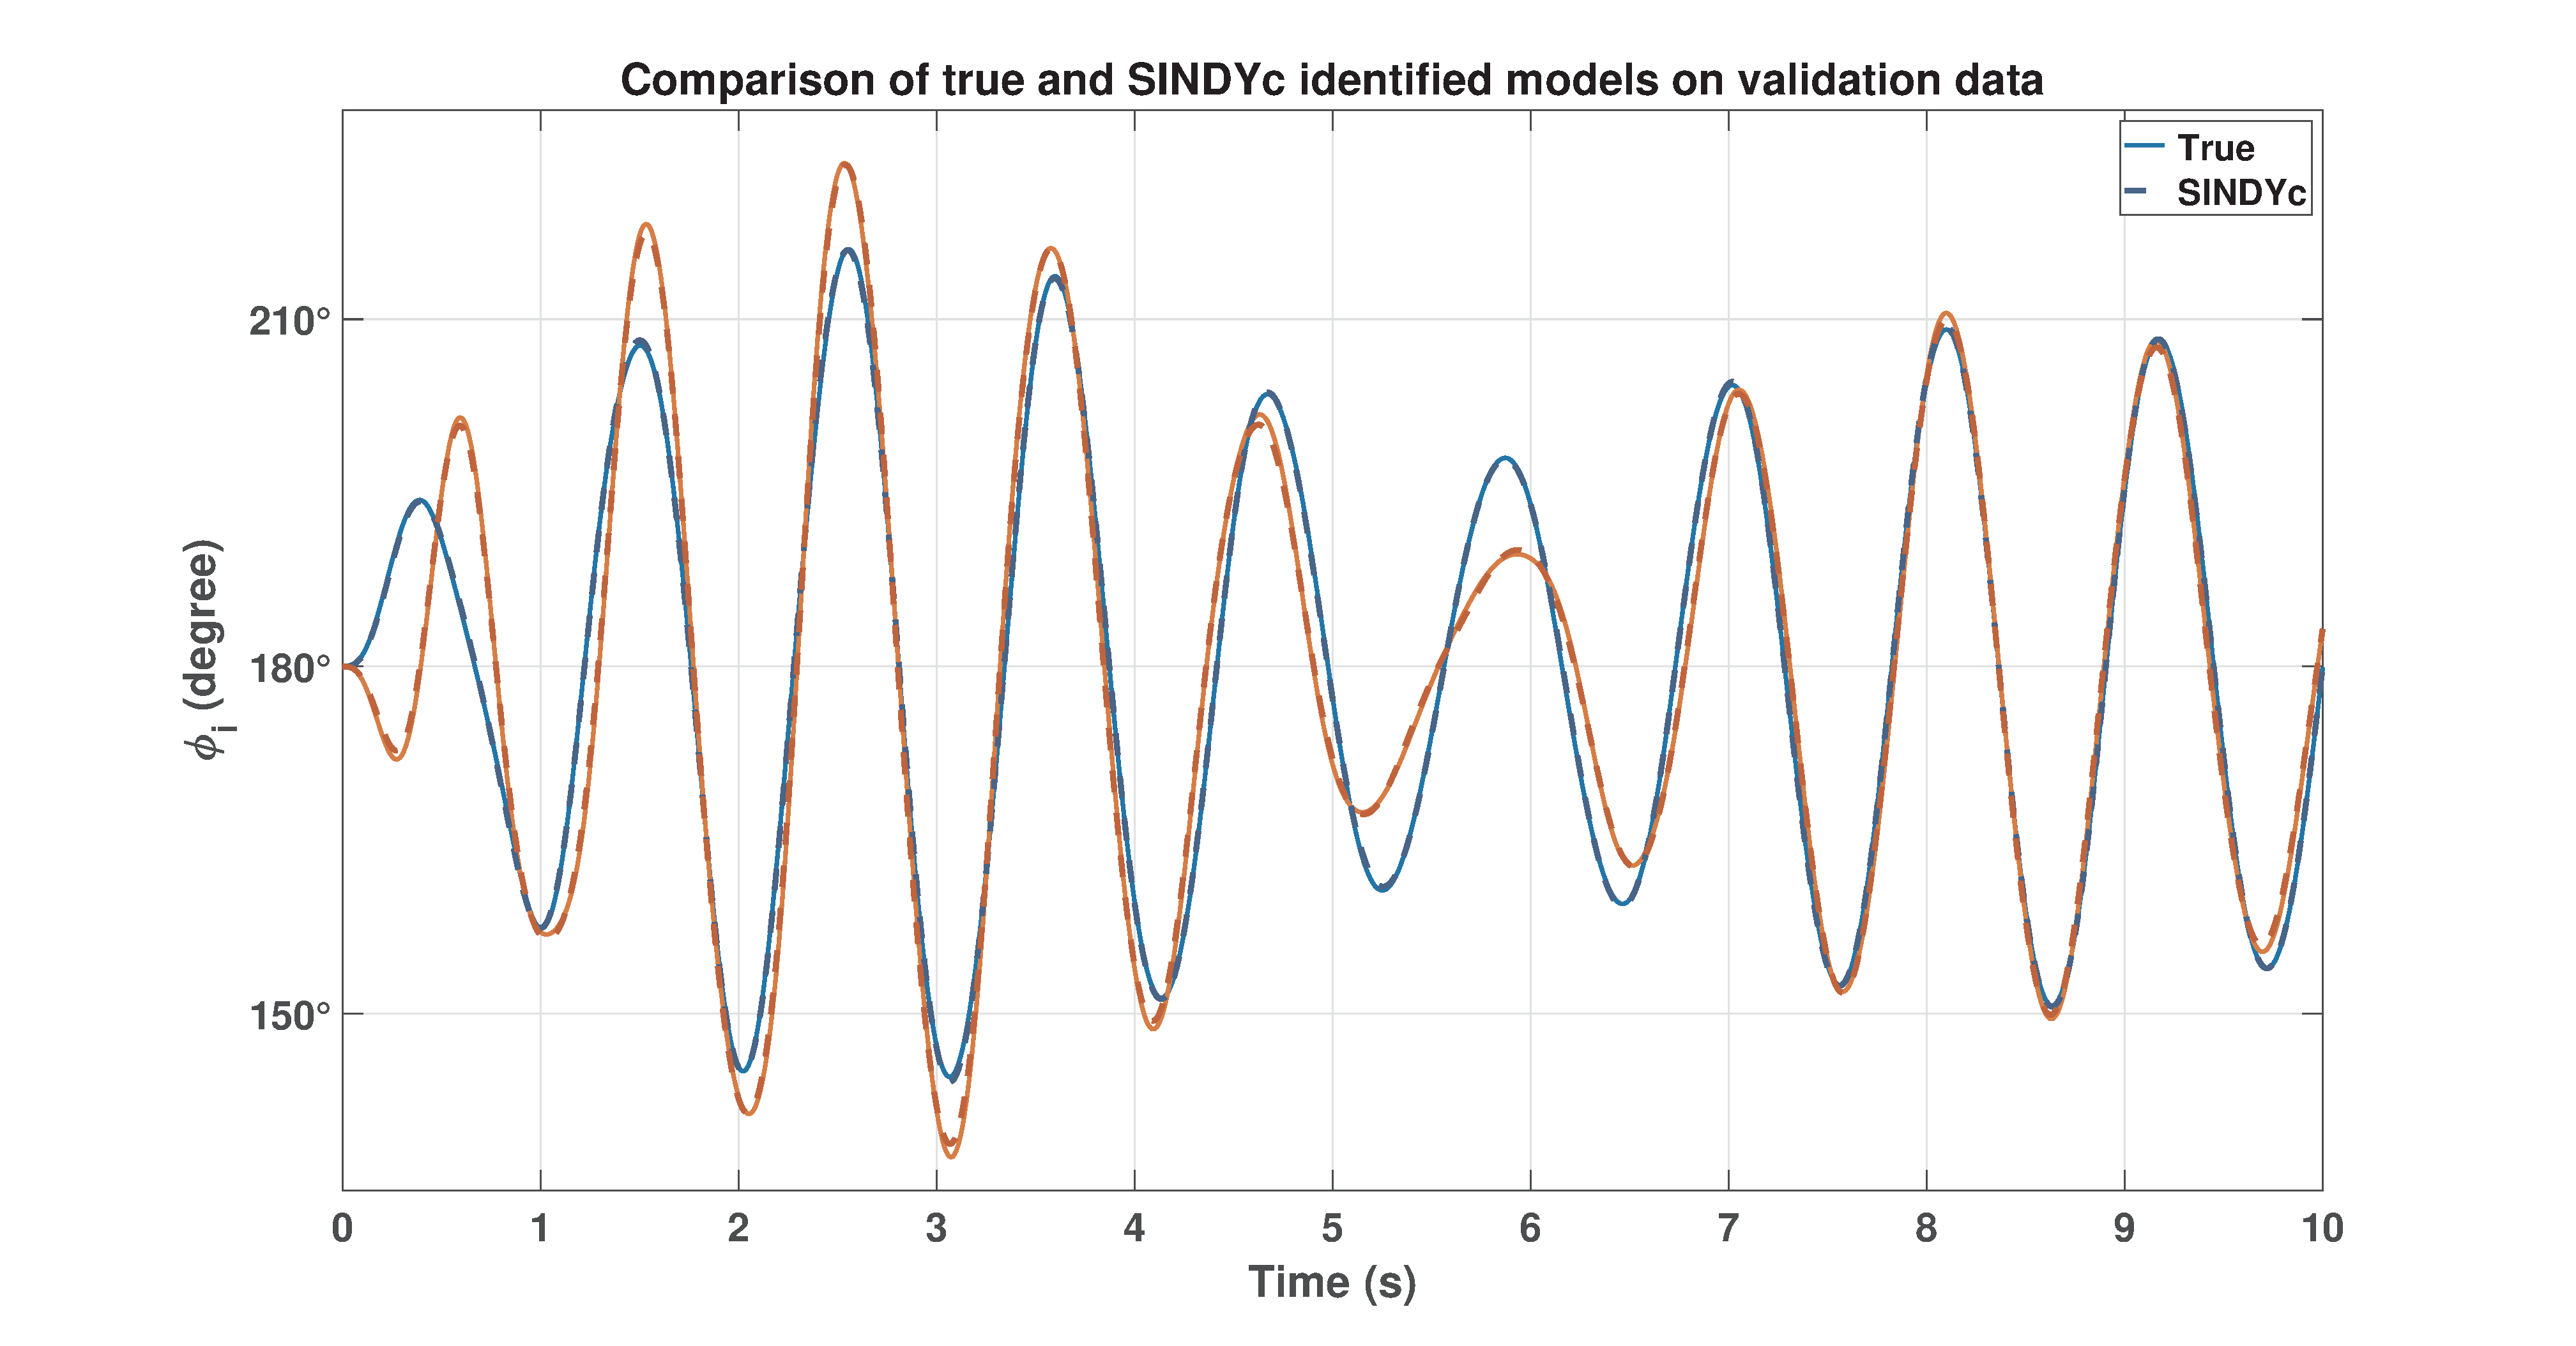
\includegraphics[width=1\linewidth]{figures/MultTrajVal_2_0_1}
    \caption{Identification with multiple trajectories and $\mathbf{\Psi_3}$ on validation data}
    \label{fig: MultTrajVal}
\end{figure}
% 
\newpage
Figures \ref{fig: inputTrainVal}, \ref{fig: SingleTrajValCombo} and \ref{fig: MultTrajValCombo} visualize forcing functions and the consequent predictions with a slightly different forcing function from earlier but still within the range defined by (\ref{Eq:Forcing}). The forcing function used here for training is a chirp signal with a constant frequency. Again, it is seen that model approximated from data generated by multiple trajectories performs better.
\begin{figure}[H]
    \centering
    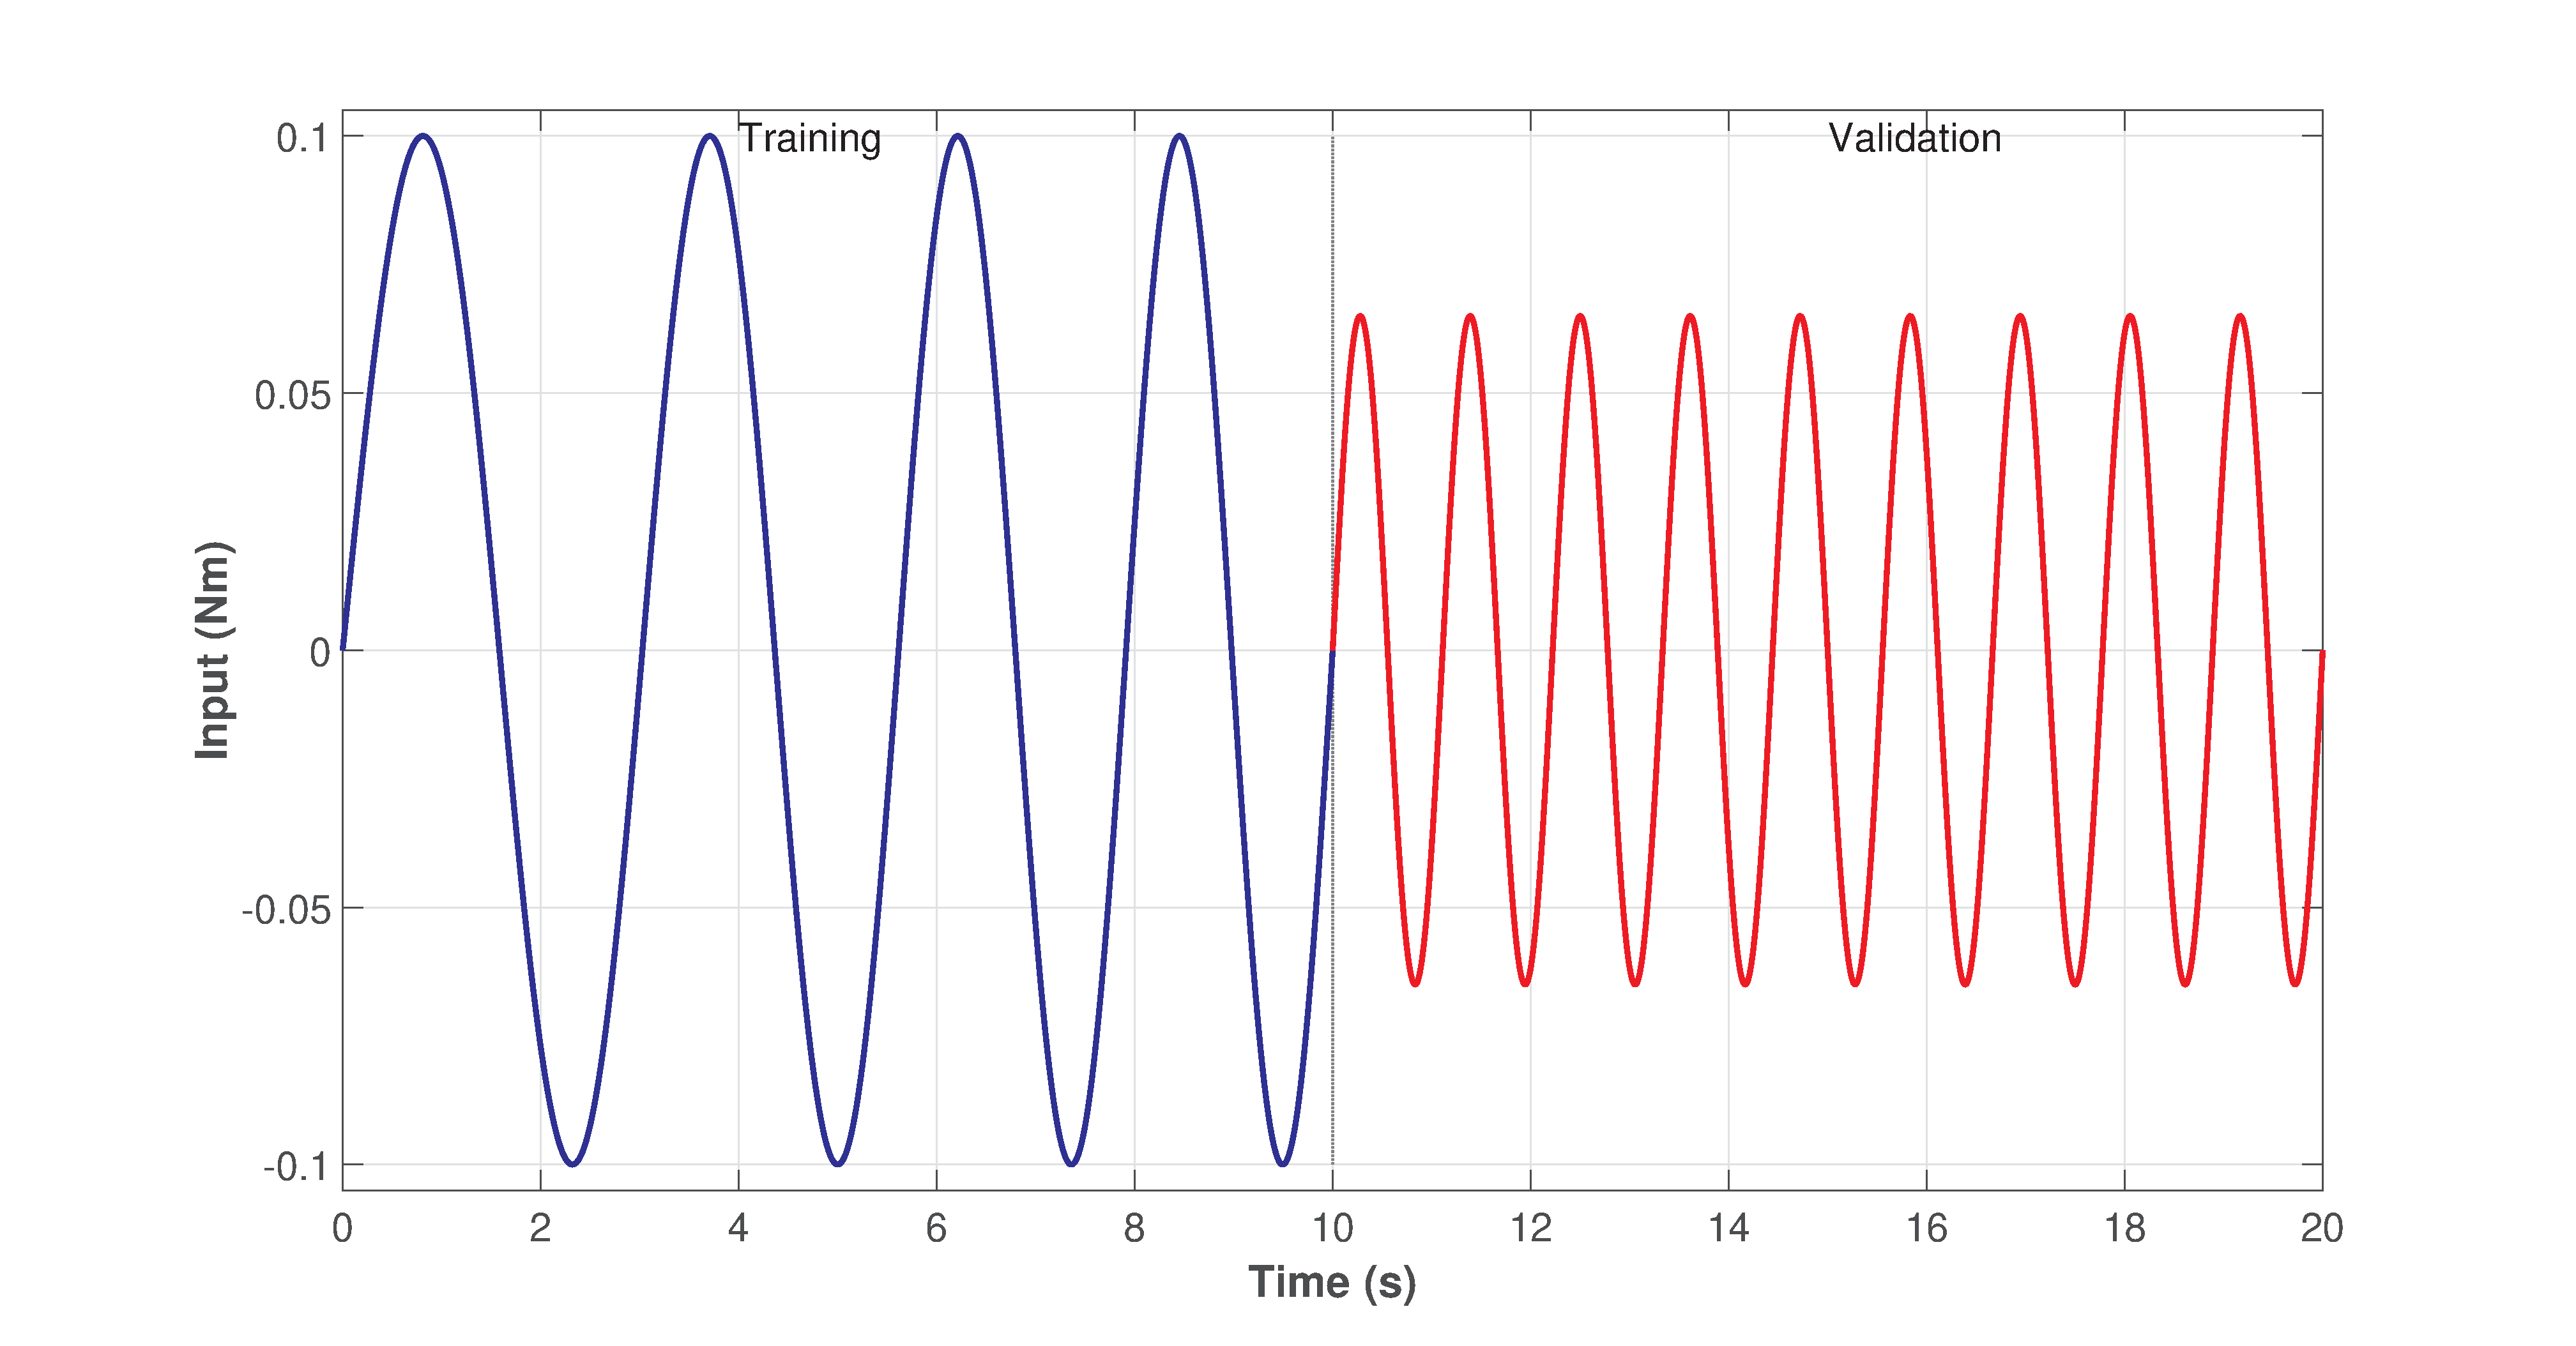
\includegraphics[width=0.85\linewidth]{figures/Input}
    \caption{The training and validation inputs}
    \label{fig: inputTrainVal}
% \end{figure}
\vspace{0.005em}
% \begin{figure}[ht]
    \centering
    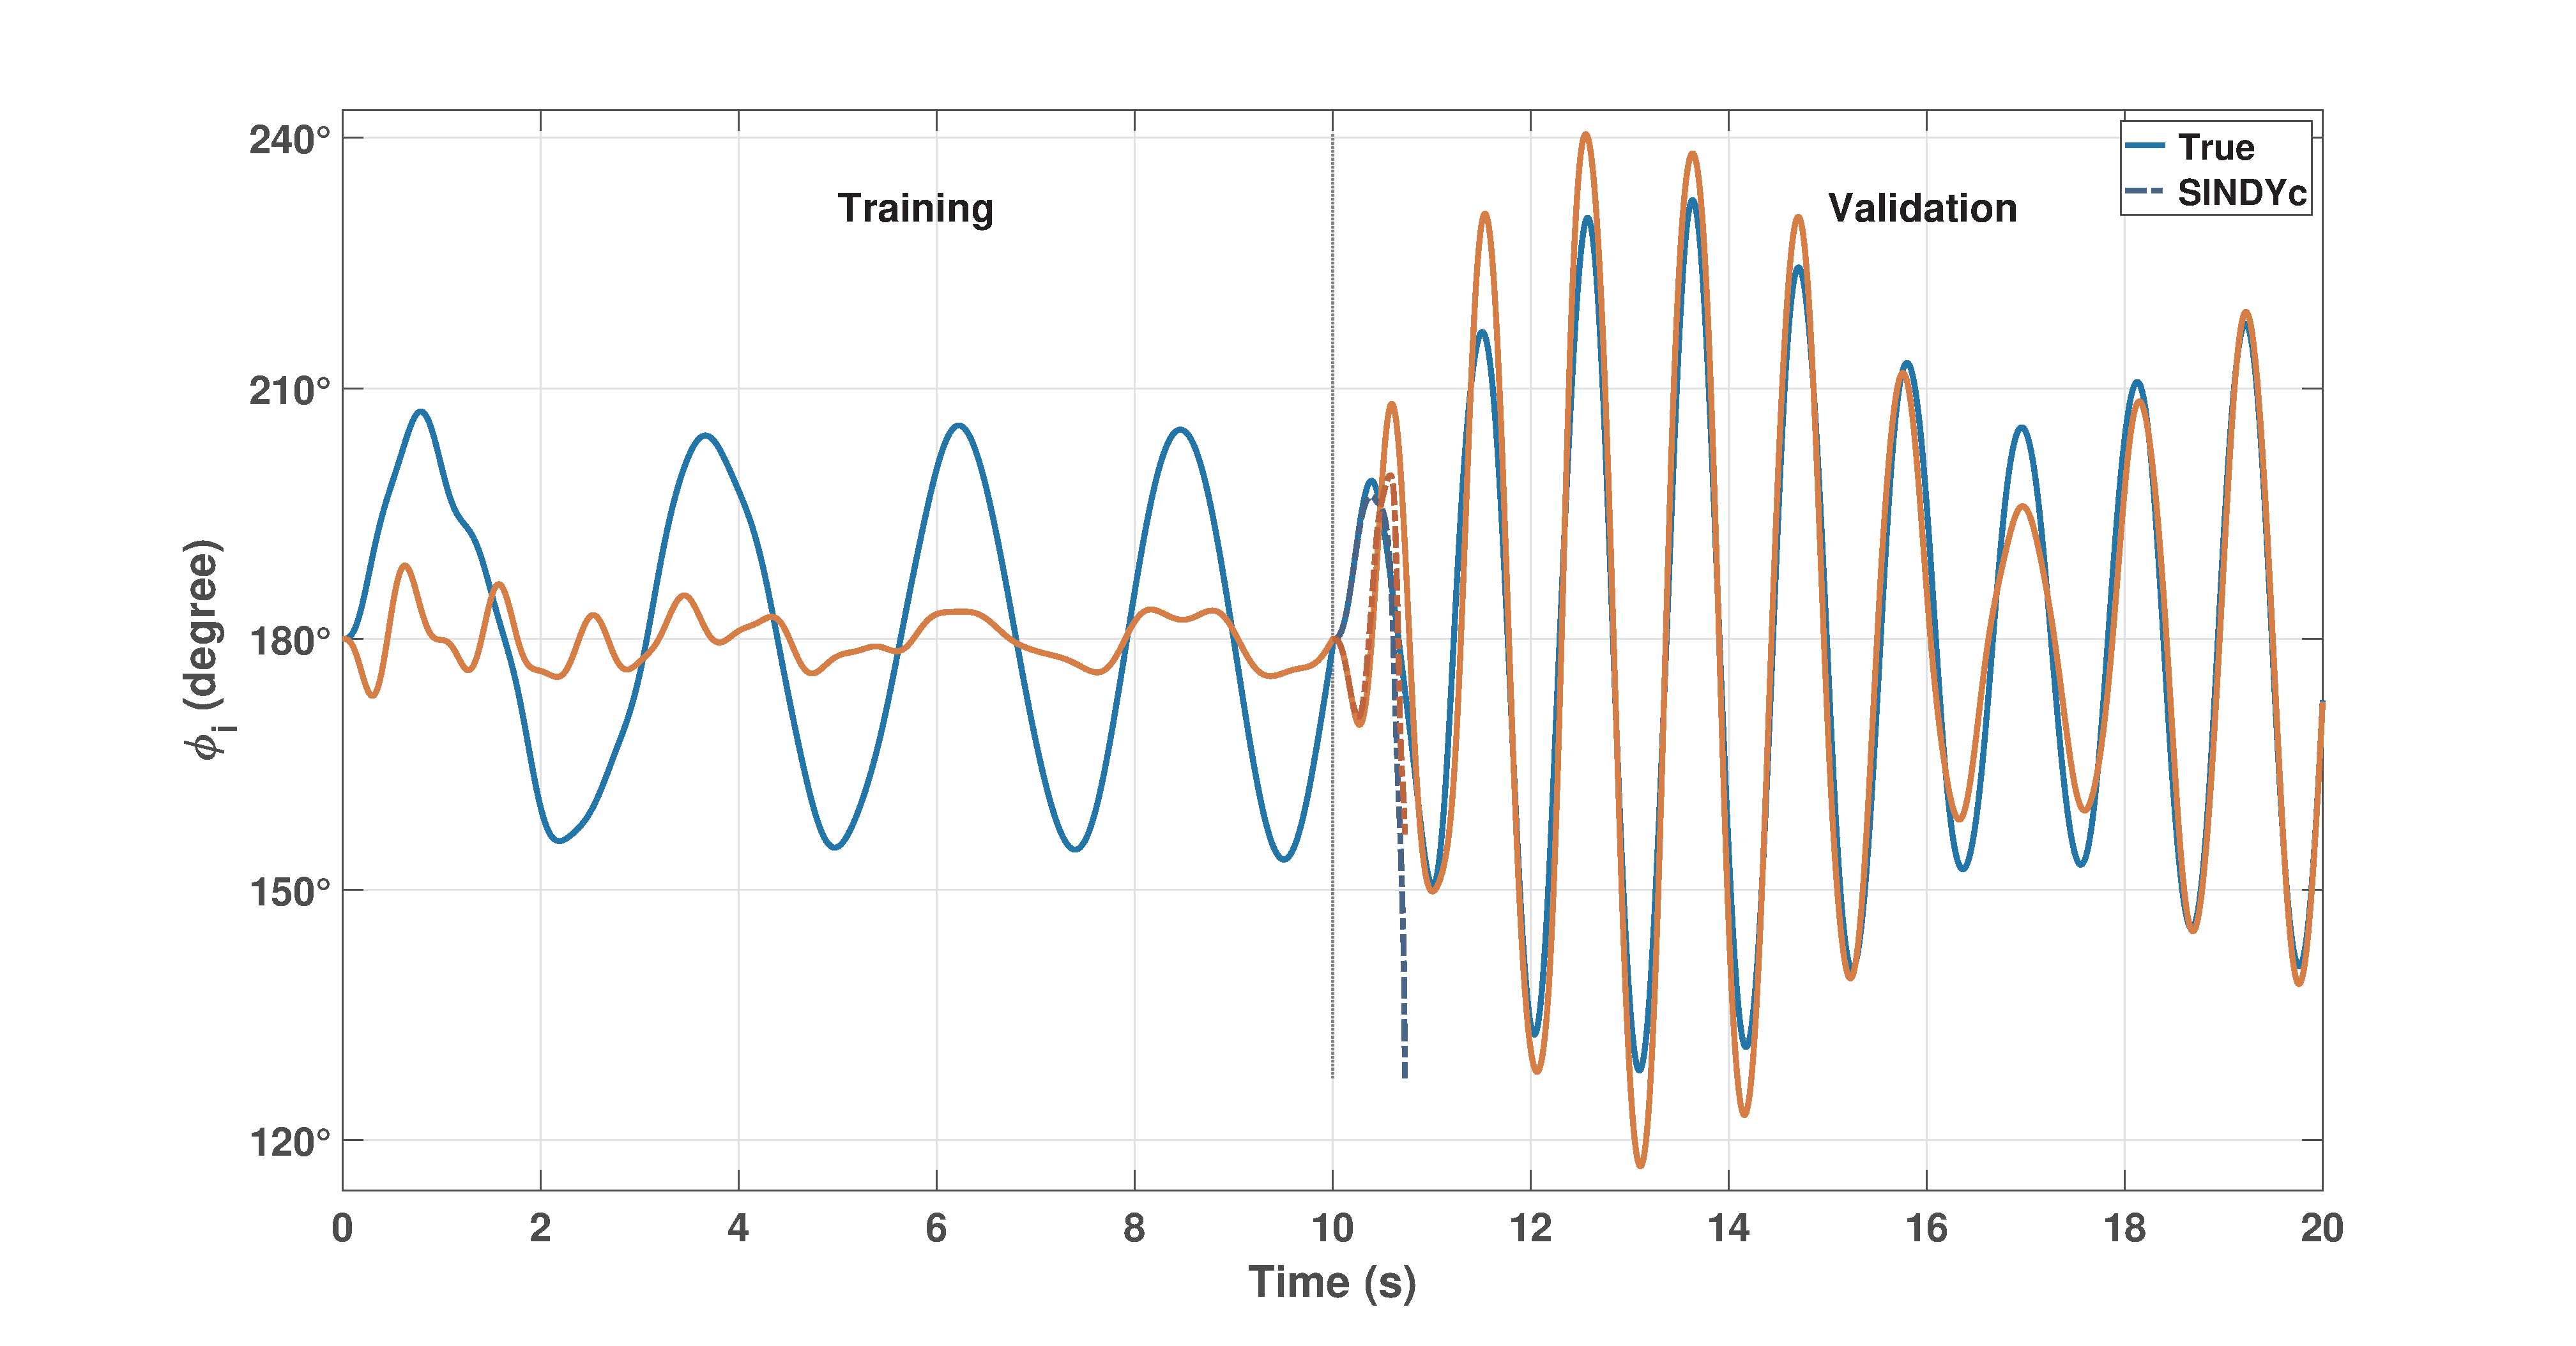
\includegraphics[width=0.85\linewidth]{figures/VizSingleTrajVal_2_0_1}
    \caption{Visualization of the validation with single trajectory and $\mathbf{\Psi_3}$}
    \label{fig: SingleTrajValCombo}
% \end{figure}
\vspace{0.005em}
% \begin{figure}[ht]
    \centering
    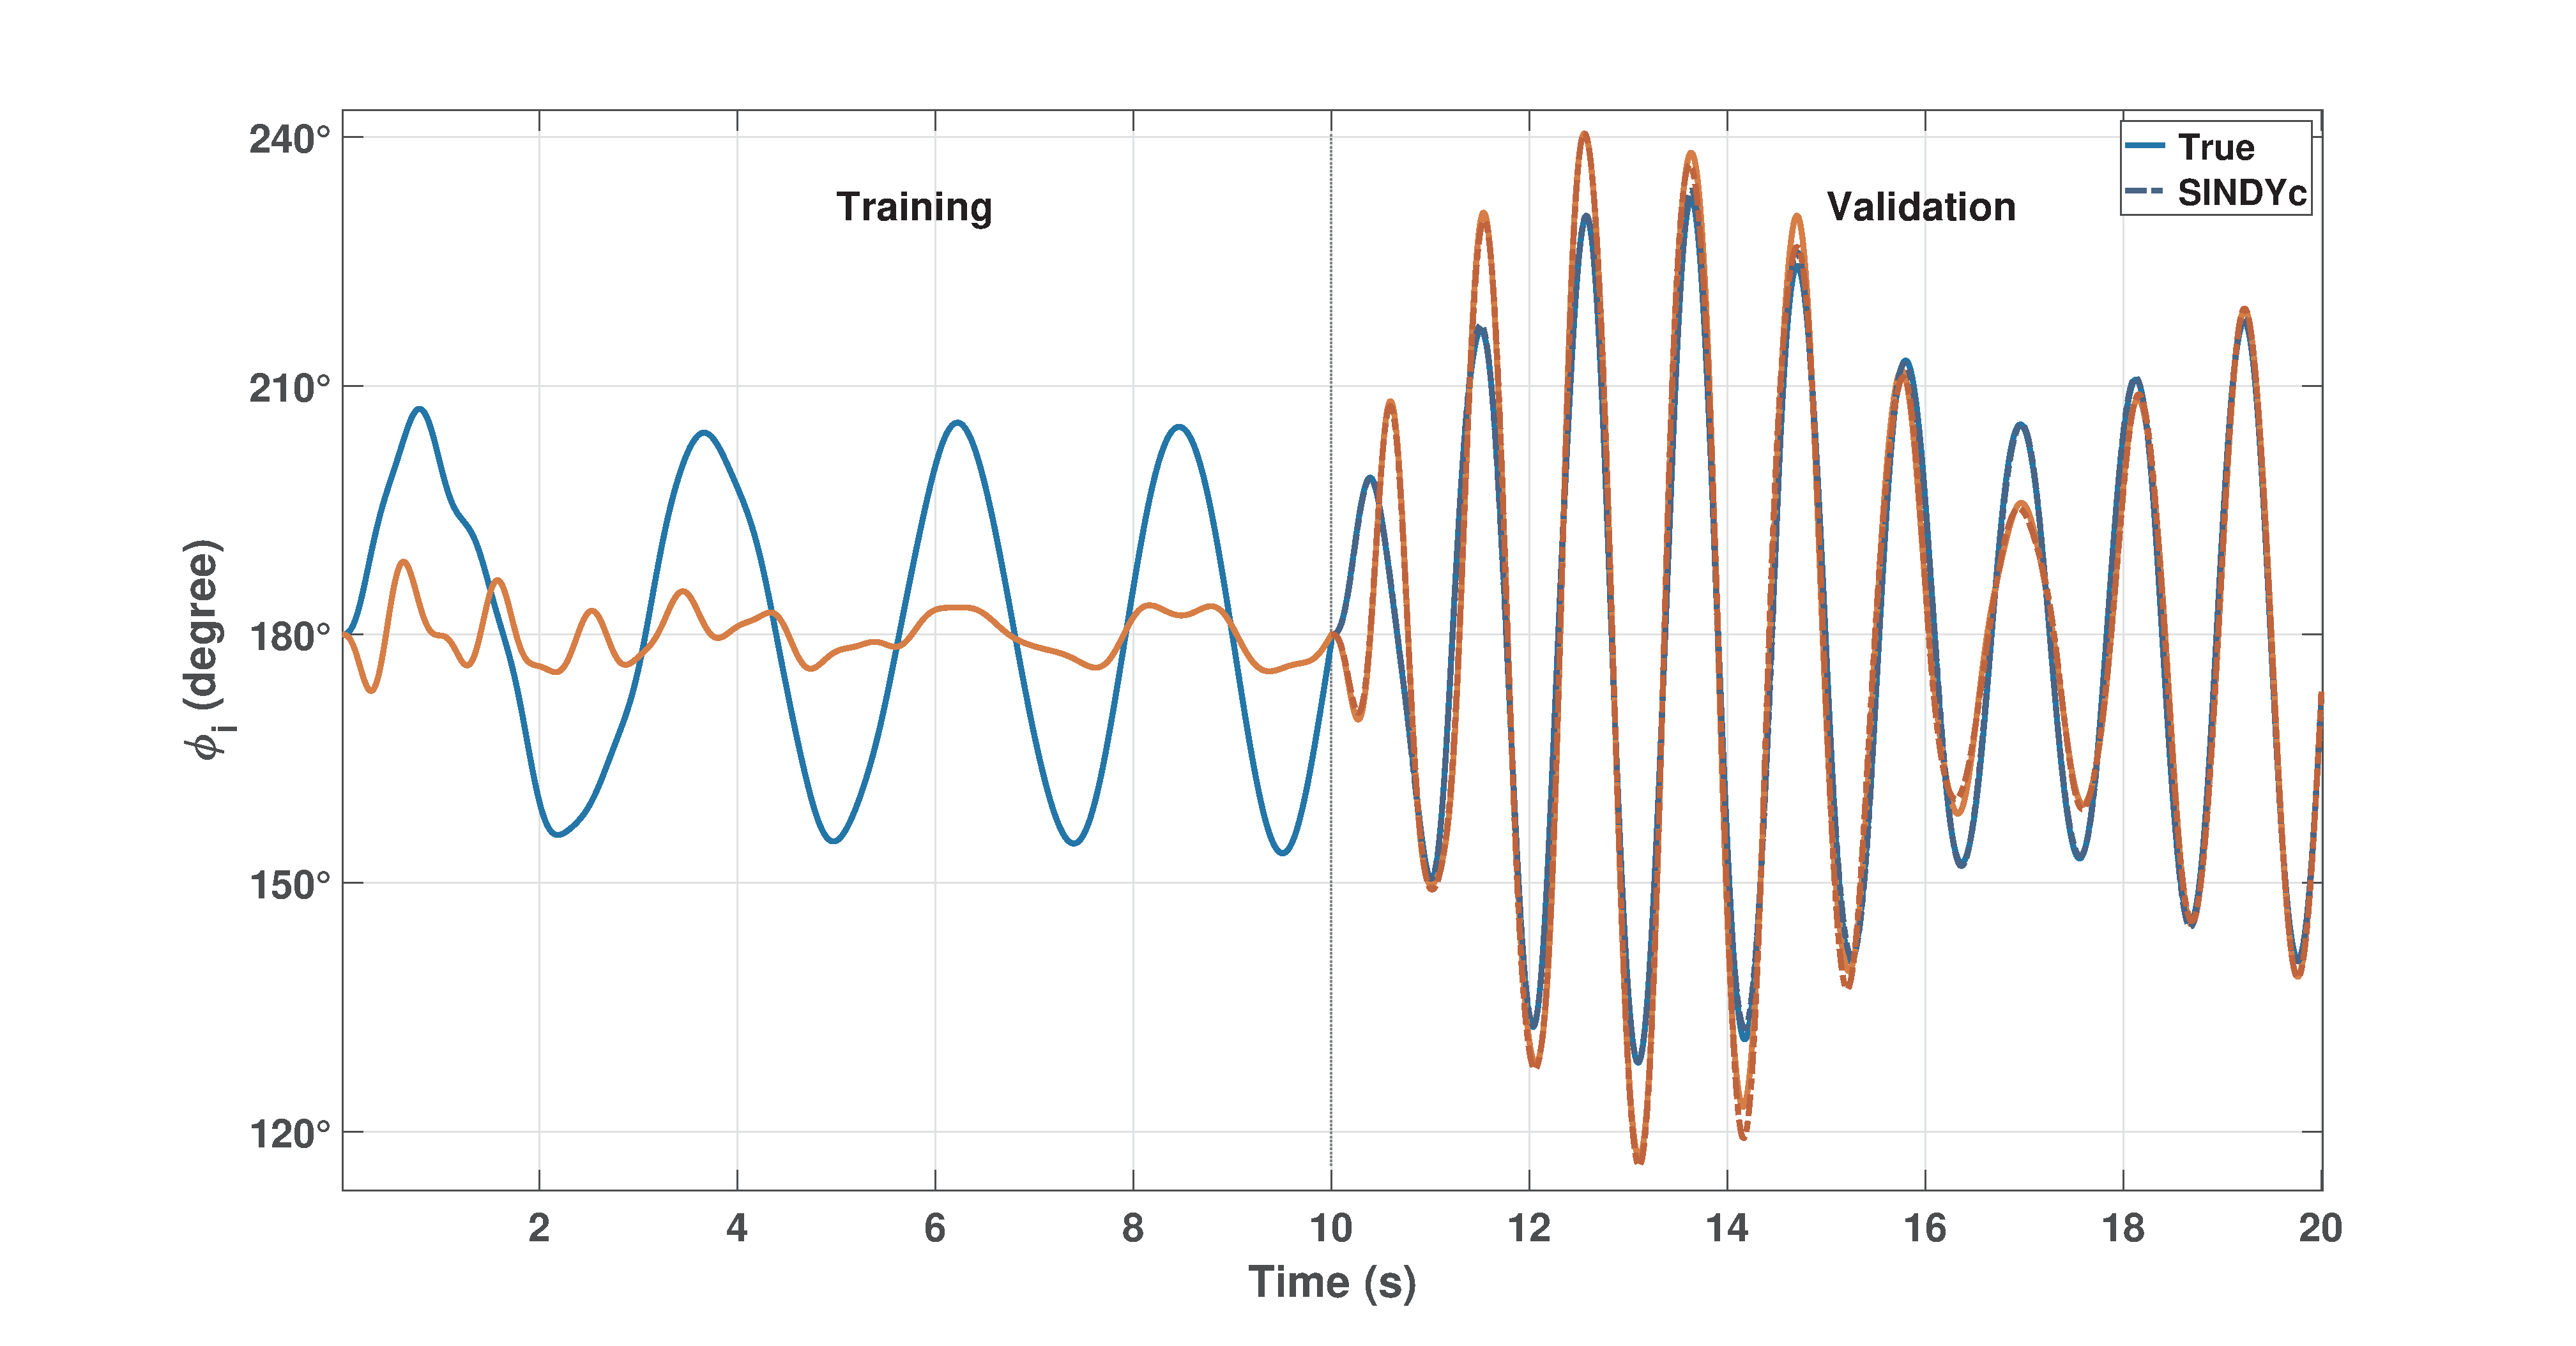
\includegraphics[width=0.85\linewidth]{figures/VizMultTrajVal_2_0_1}
    \caption{Visualization of the validation with multiple trajectories and $\mathbf{\Psi_3}$}
    \label{fig: MultTrajValCombo}
\end{figure}
% 
\newpage
The predictions fit the true trajectories for a specific choice of candidate functions, $\mathbf{\Psi}_3$, in the above figures. Some or all of the linear or nonlinear functions in this set of candidate functions may form the set of observables required to compute the Koopman operator, generating a linear approximation of the underlying nonlinear system. The sparse coefficients matrix $\mathbf{\Xi}$ is a good indicator of such dominant linear or nonlinear functions which can then be considered as observables. It is important to note that the choice of candidate functions, and consequently, the choice of observables is highly subjective, and there are no fixed rules/methods to choose them. Some of the ways have been discussed in Chapter \ref{Chapter:Intro}. Figure \ref{fig: MultTrajVal2} illustrates the effect of choice of candidate functions. The set of candidate functions used in this case to generate the $\mathbf{\Xi} $ is $\mathbf{\Psi}_2$ which is a set of polynomials up to a second degree. It is seen that $\mathbf{\Psi_2}$ can only approximate the dynamics in a small region around the stable equilibrium after which the predicted trajectories do not behave like the reference trajectory. On the other hand, in Figure \ref{fig: MultTrajVal}, the predicted trajectories closely match the true trajectory. This shows that as one moves away from the desired equilibrium point, the initial state vector needs to be augmented with other nonlinear functions to enable predictions over longer time spans and/or over a larger range.
% 
\begin{figure}[H]
    \centering
    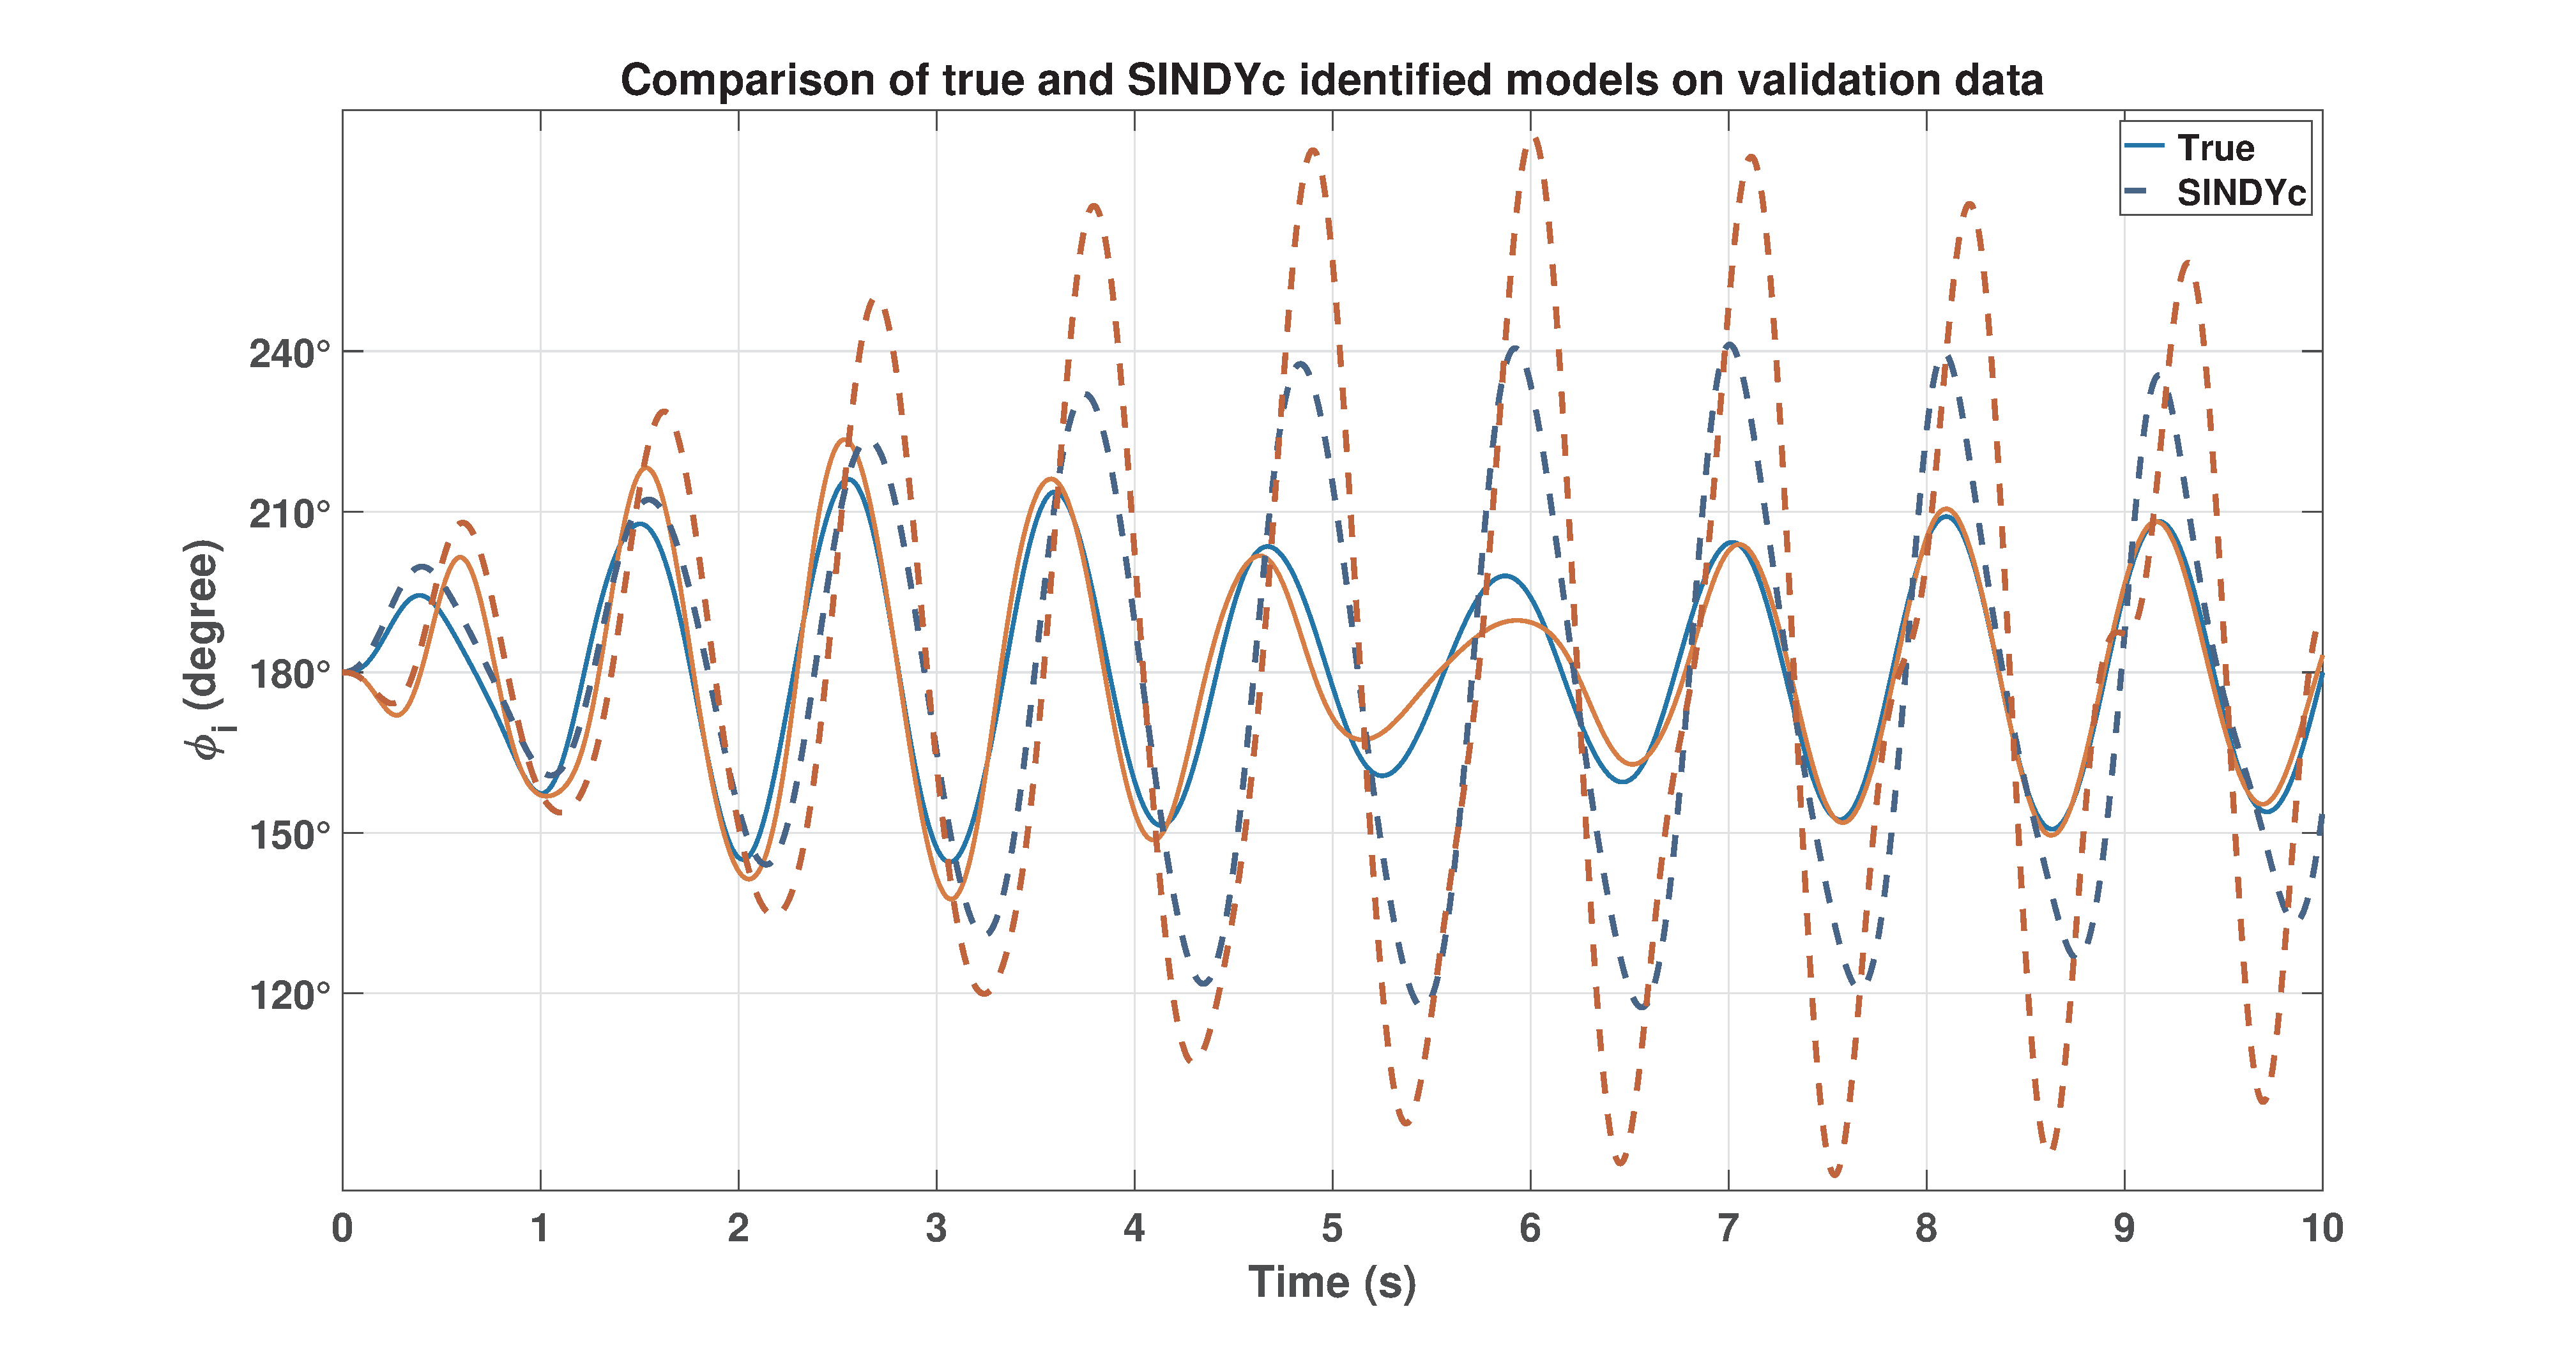
\includegraphics[width=1\linewidth]{figures/MultTrajVal_2_0_0}
    \caption{Identification with multiple trajectories and $\mathbf{\Psi_2}$ on validation data}
    \label{fig: MultTrajVal2}
\end{figure}
% 
The following section applies the knowledge obtained from this section to efficiently synthesize a data-driven controller for the ADIP to track a closed-loop reference trajectory.\newpage
\subsection{Tracking}
\label{sec:ResultsTrack}
One can safely say that data-driven control is majorly dependent on the setting up of data, computation of data-driven linear matrices (the finite approximation of the Koopman operator) and stands mostly solved once the parameters of data generation are decided upon. Once the linear matrices are generated, synthesizing a controller follows the same procedure as any linear model. In this thesis, all the controllers used were tuned using a genetic algorithm that simplifies finding the right combination of tuning parameters. \par 
In the following results, for the sake of comparison, the tuning matrices used for all the presented controllers with the exception of the qLMPC are the same with $\mathbf{Q} = \textup{diag}(85.38,~15.32,~0,~0.44)$ and $\textup{R} = 1.4$. Additionally, the penalty on the integrated error state is $\textup{Q}_i = 300$ and the penalty on the final state for MPC is, $\textup{Q}_N = Q$.\par
This section applies the insights and observations from the previous section in tracking a reference trajectory in the up-up configuration of ADIP. The full-state measurements are collected as discussed previously in Section \ref{sec:Results_ident} (see Figures \ref{fig:ReferenceTraj}, \ref{fig:InputSignal}) assuming that a closed-loop controller is available to stabilize the system. Also, the input torque is bounded by the maximum allowable range $[-2.5~~2.5]$Nm.\par
Figure \ref{fig: LQi_comp} compares the tracking performance of a linear quadratic regulator with integral action on the \textit{local} model generated by Jacobian linearization of the nonlinear dynamics at the point of unstable equilibrium ($\phi_1 = \phi_2 = 0^{\circ}$) against the Koopman model generated solely from data with the observables vector $\mathbf{\Psi}_1 = [\phi_1~\phi_2~\Dot{\phi}_1~\Dot{\phi}_2]^\top$, i.e, only the linear measurements of state. It was observed that the linear measurements of the state were enough to track a reference up to $40^{\circ}$ with an LQi controller, which also agrees with the LQi applied to the local model. Furthermore, Fig. \ref{fig: LQi_cost} visualizes the quadratic cost $J$ in Eq.~\ref{eq:Costfunc}. It can be seen that costs for the local model and the data-driven model are comparable and in fact, the former's cost was a little bit higher than of the latter. Importantly, it must be noted that the Koopman model was generated solely from data with almost no assumptions made about the system. \par
In the figures \ref{fig: LQi_comp}, \ref{fig: MPC_all}, (\textcolor{blue}{\textbf{--}}) and (\textcolor{red}{\textbf{--}}) represent the trajectories of $\phi_1$ and $\phi_2$ generated by the local model, respectively. Consequently, (\textcolor{blue}{\textbf{-~-}}) and (\textcolor{red}{\textbf{-~-}}) represent the trajectories of $\phi_1$ and $\phi_2$ generated by the Koopman model, respectively.
% % 
\begin{figure}[H]
    \centering
    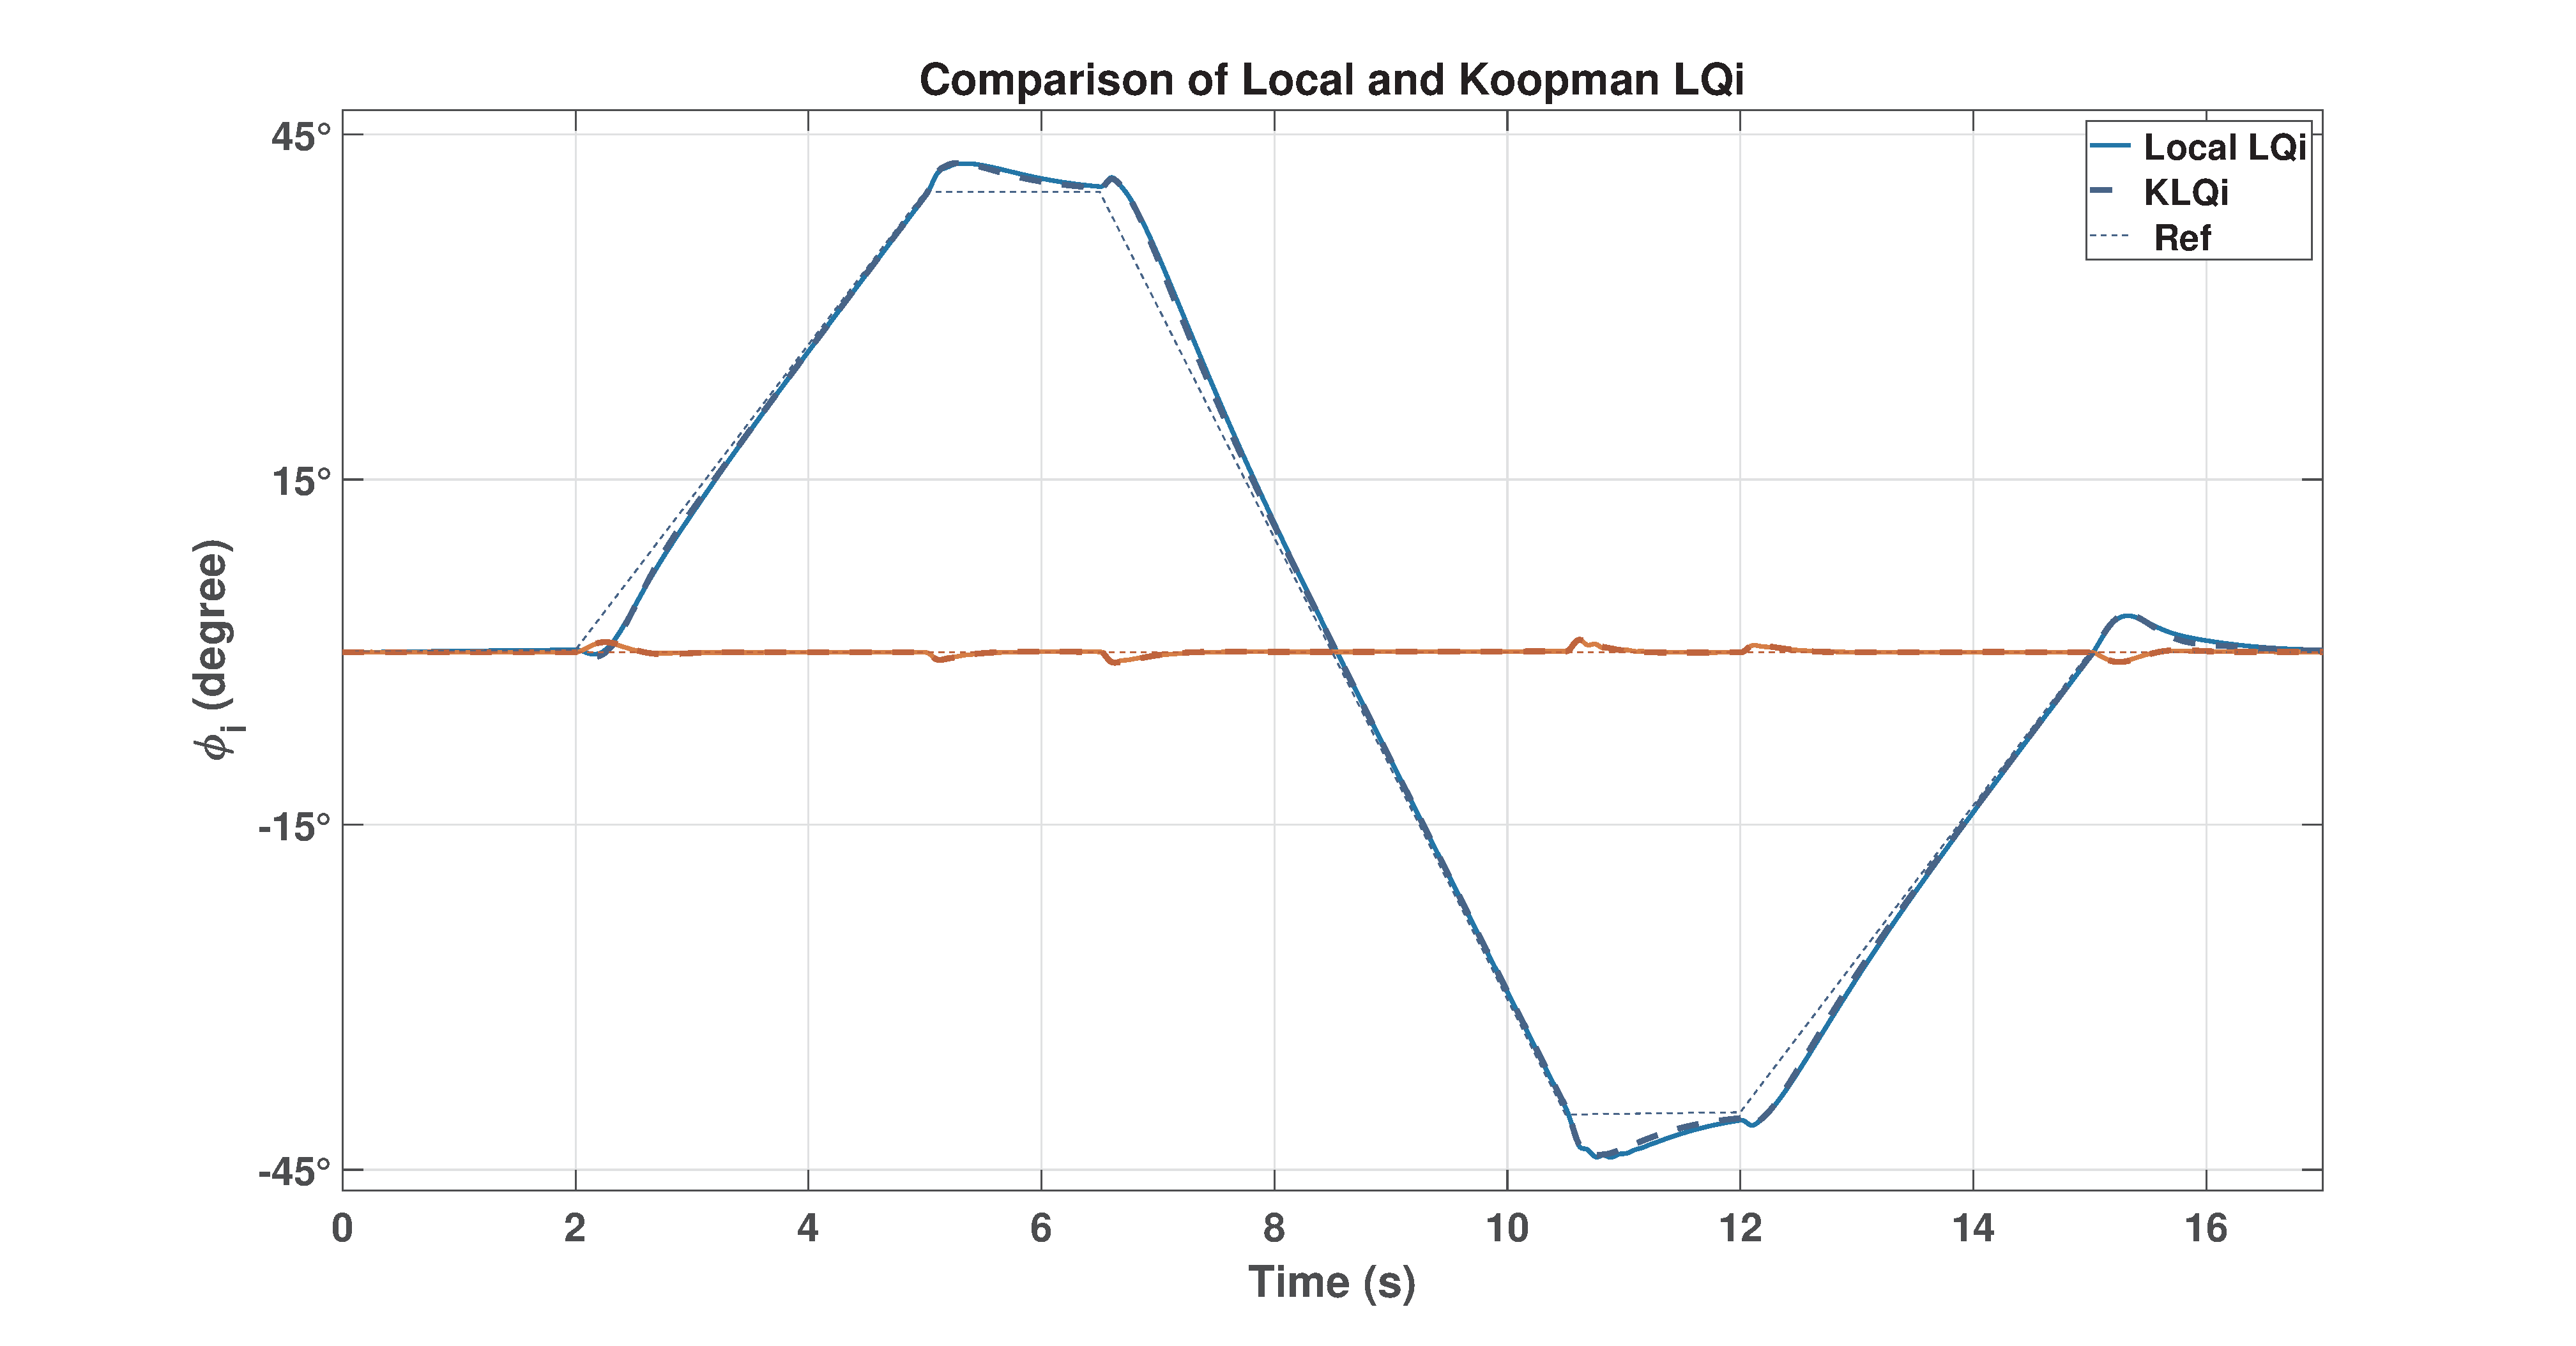
\includegraphics[width=1\linewidth]{figures/LQi_comp_5ms}
    \caption{Comparison of LQi applied to locally linearized model versus Koopman model with $\mathbf{\Psi_1}$}
    \label{fig: LQi_comp}
\end{figure}
% 
\begin{figure}[H]
    \centering
    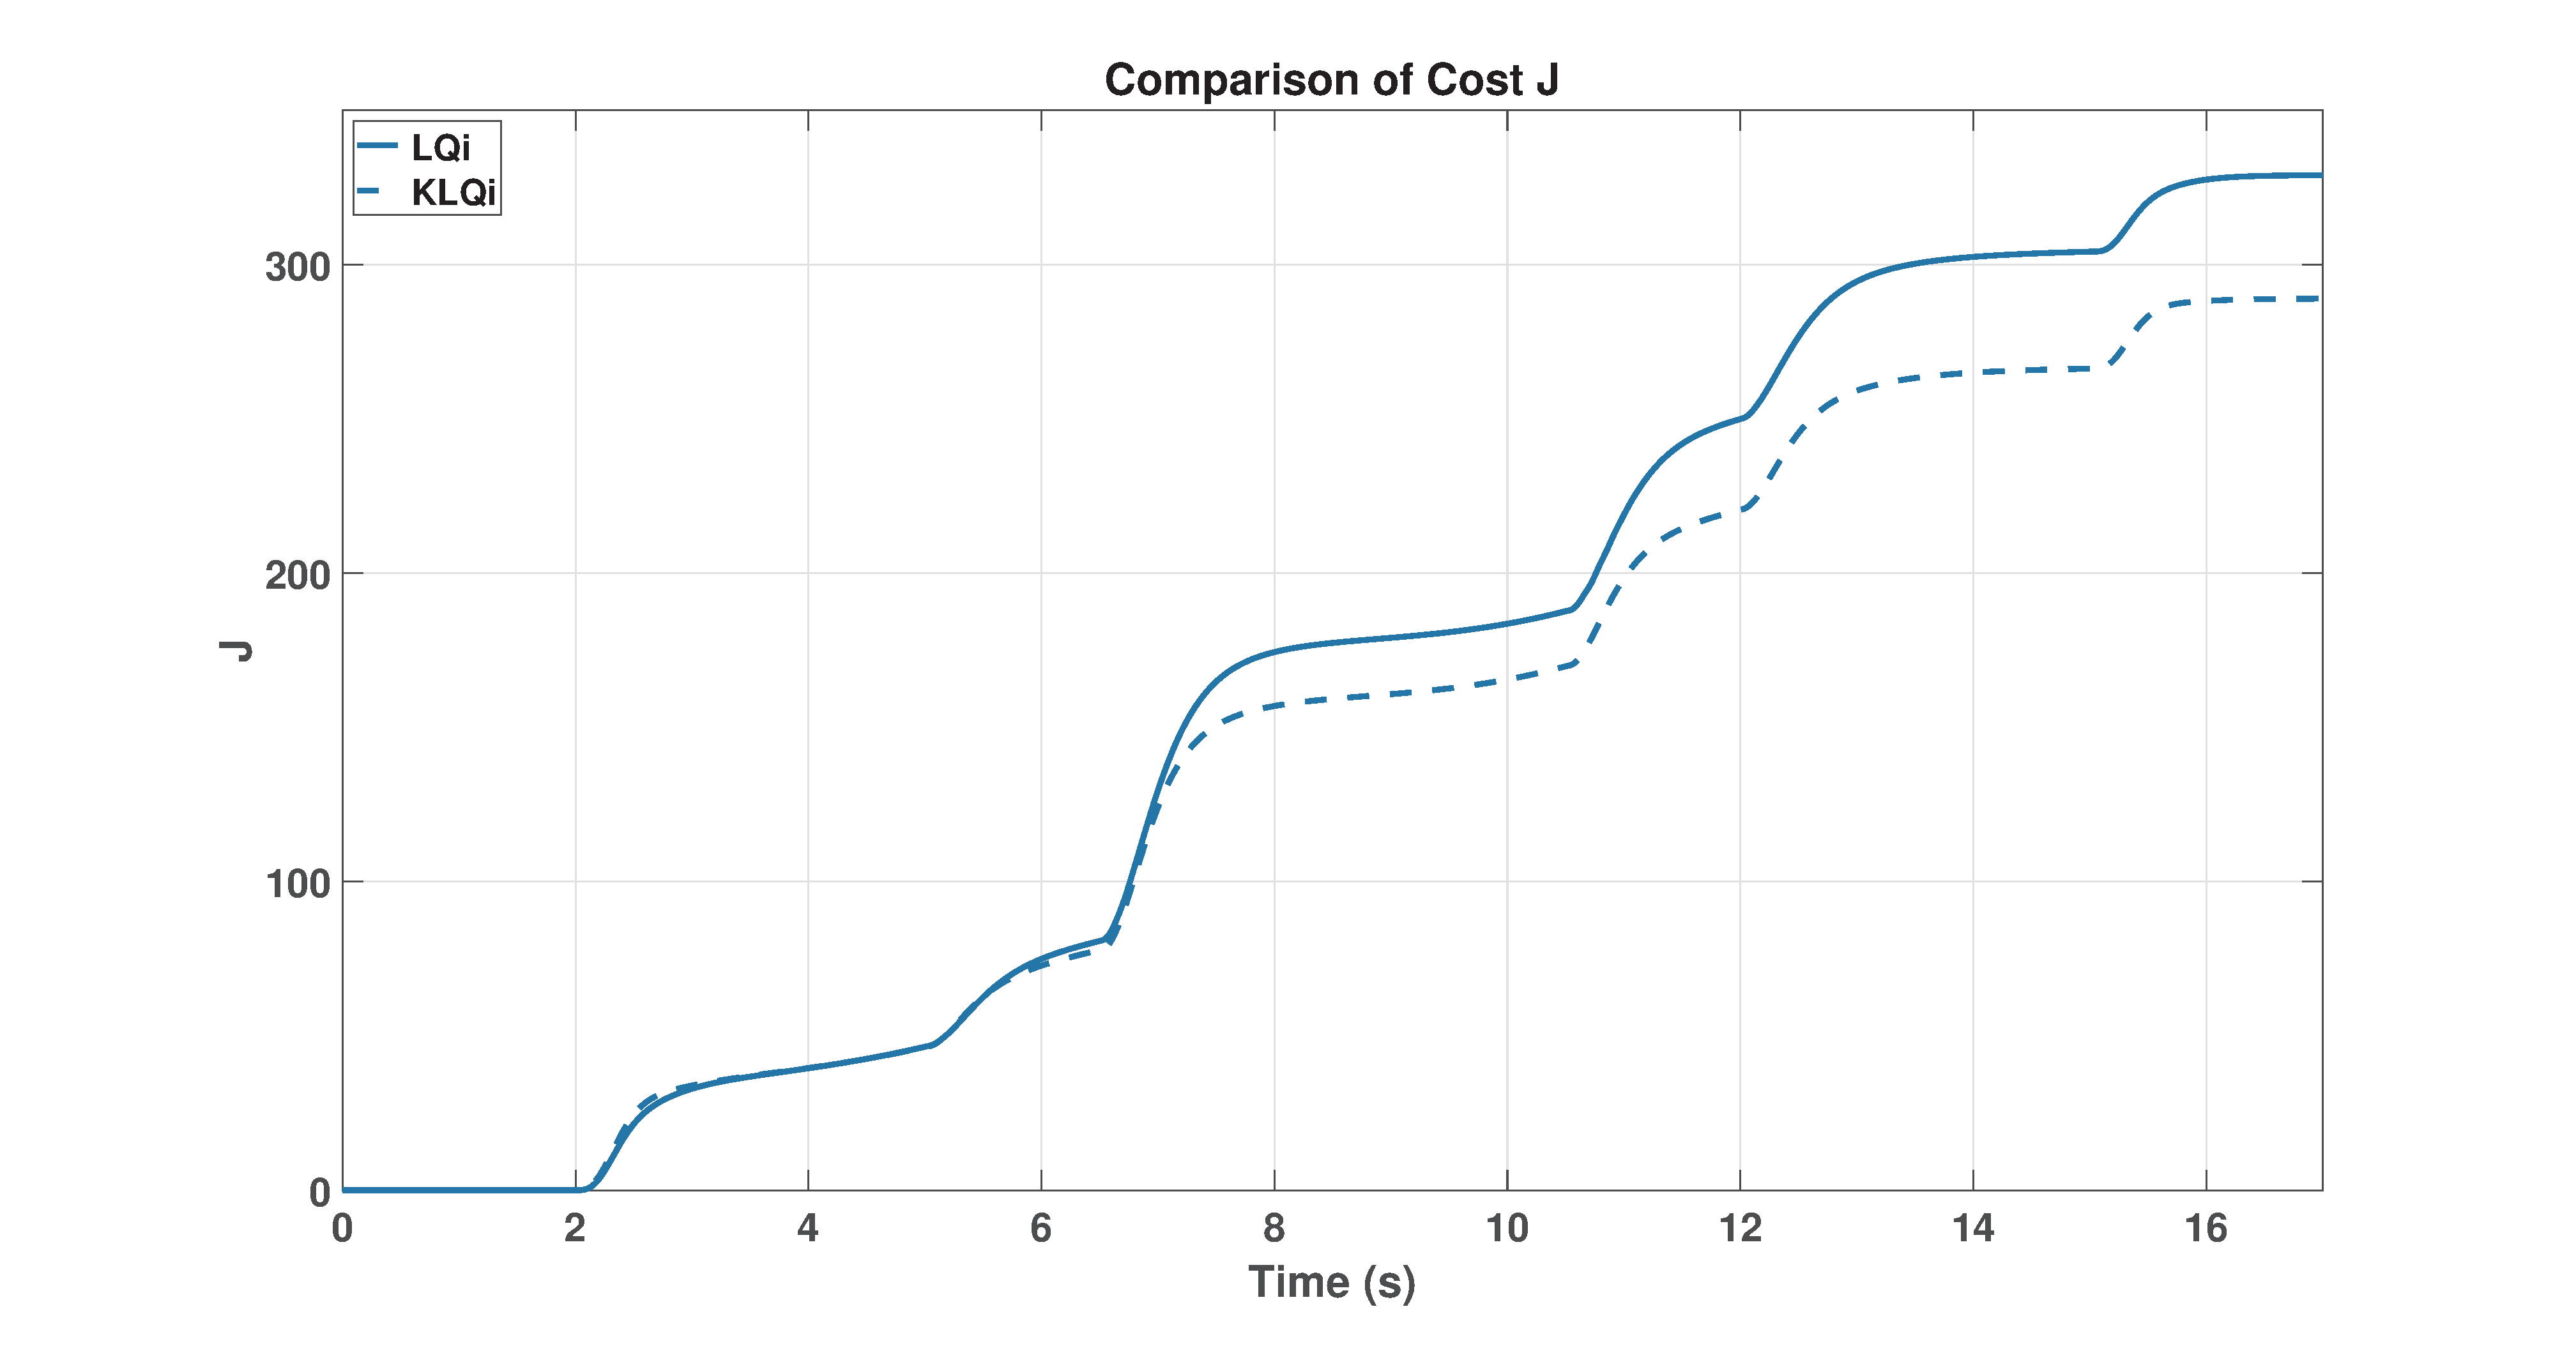
\includegraphics[width=1\linewidth]{figures/CostsLQi_5ms}
    \caption{Comparison of quadratic cost function $J$ for closed-loop tracking with local and Koopman operator approximated model}
    \label{fig: LQi_cost}
\end{figure}
% 
Next, a model predictive controller with a prediction horizon of $N_p = 200$, i.e. a prediction of 1 second into the future, was designed for the above-generated models. It was observed that the range of tracking could be increased from $40^{\circ}$ to $45^{\circ}$. This was expected as MPC almost always performs better than the linear quadratic regulator, especially more so in tracking problems. This is because, as opposed to the optimization of the quadratic cost function over an infinite time horizon as is the case with LQR (\ref{eq:Costfunc}), the MPC optimizes the cost function over a finite time horizon (\ref{eq:MPCcostfunction}) and repeatedly computes the optimal input. As a result, the controller can generate optimal control inputs valid for only a small fixed horizon instead of optimal control inputs that are valid over a very long period of time as in the case of a linear quadratic regulator. However, this comes at a cost. The optimal LQR input is computed offline and does not change during the process. In contrast, in MPC, the optimal input is computed online and, therefore, depends on the computer's computational capabilities. This cost can, however, be greatly reduced by formulating the MPC problem in a dense form (Eqs. \ref{eq:NstepComp} and \ref{eq:MPCdense}) as proposed by Korda et al. \cite{MPC_Korda}. The matrices $\mathbf{\Bar{A}}$ and $\mathbf{\Bar{B}}$ can be pre-computed offline, and one only needs to update the current state vector $\mathbf{x}_k$ online. This greatly reduces the computational effort and renders the MPC as feasible as the LQi in terms of implementation. Moreover, this dense formulation (Eq. \ref{eq:MPCdense}) is independent of the state's dimension and therefore, augmenting a state with nonlinear observables does not significantly affect the computational time of the MPC.  Figure \ref{fig: MPC_all} compares the local model's tracking performance against the Koopman model. Again, the overall quadratic cost functions are similar for local and Koopman models.
% 
\begin{figure}[H]
    \centering
    \includegraphics[width=1\linewidth]{figures/MPC_all_5ms}
    \caption{Comparison of MPC applied to local model versus Koopman model with $\mathbf{\Psi_1}$}
    \label{fig: MPC_all}
\end{figure}
% 
Table~\ref{tab:Exec_1} presents the corresponding computation times for the local and Koopman models executed with a sampling time of 5ms and 10ms. It should be noted that the controllers for the models generated from data sampled every 10ms are different from the controllers tuned for models generated from data sampled every 5ms. Both the controllers were GA-tuned to de-emphasize the effect of human bias. The comparison between the sampling times is made to highlight the trade-off between computation time and the model-controller combinations' performance. Table~\ref{tab:RMSE_1} presents the relative root-mean-square-error (in \% error w.r.t the reference trajectory of $\phi_1$) for the model-controller combinations explored until now in this section.
% 
\begin{table}[H]
    \centering
    \begin{tabular}{lcc}
         \toprule
                                  & \multicolumn{2}{c}{Average execution time~(ms)}\\
        \cmidrule{2-3}
         Model - Controller       & $T_s = 5$ms  & $T_s = 10$ms\\
         \midrule
         Local - MPC               & 0.56        & 0.17\\
         $\textup{KO}_1$ - MPC    & 0.59         & 0.18\\
         \bottomrule
    \end{tabular}
    \caption{Average execution time~(ms) of the MPC algorithms for different sampling times}
    \label{tab:Exec_1}
\end{table}
% 
\begin{table}[H]
    \centering
    \begin{tabular}{lcc}
         \toprule
                                            & \multicolumn{2}{c}{RMSE(\%)}\\
        \cmidrule{2-3}
         Model - Controller                  & $T_s = 5$ms & $T_s = 10$ms\\
         \midrule
         Local - LQi                         & 6.60       & 7.13\\
         $\textup{KO}_1$ - LQi               & 6.32       & 6.59 \\
         Local - MPC                         & 0.69       & 2.84\\
         $\textup{KO}_1$ - MPC               & 0.53       & 3.53\\
         \bottomrule
    \end{tabular}
    \caption{RMSE(\%) of tracking errors for different sampling times}
    \label{tab:RMSE_1}
\end{table}
% 
As observed in Section \ref{sec:Results_ident}, the choice of observables also plays an important role in approximating the system's dynamics farther away from the point of linearization. While there is no rule book which exactly governs the selection of such observables, it is often possible to work with proven basis functions used to approximate nonlinear dynamics in general. The only issue is that this space of observables spans infinite dimensions and therefore, one may or may not find the `correct' observables, which will serve the purpose. It is also important to note that not all nonlinear functions of the state approximate the Koopman operator. Some `observables' may even corrupt the system and/or drive the system to instability. Examples of such approximations are given in Kaiser et al. \cite{kaiser2020datadriven}. The choice of observables, therefore, is particular to the system of interest. In this thesis, the state was augmented with radial basis functions with randomly chosen centres as previously explained in Chapter \ref{Chapter:Data}. Figure~\ref{fig: LocalKMPC12} compares the performance of an MPC controller acting on the local model, a data-driven model approximated with 4 observables ($\mathbf{\Psi}_1$) that are simply the measurements of the state and another data-driven model with the state vector augmented by 50 radial basis functions ($\mathbf{\Psi}_4$, refer Sec. \ref{Chapter:Data}), respectively to track a reference trajectory of up to $45^\circ$. \par
Furthermore, it was observed that the range of tracking with MPC applied to the data-driven model approximated with an augmented vector of RBFs could be extended to almost $60^{\circ}$. Figure \ref{fig: KPMC_comp} compares the MPC controller designed for a Koopman model approximated with observables vector $\mathbf{\Psi}_1$, which could only track a reference trajectory as good as the local model (w.r.t the range), against a Koopman model approximated with the observables vector $\mathbf{\Psi}_4$ which could extend the range of tracking by almost $50\%$ for a wise choice of observables. As a result, one may hypothesize that there may exist a set of observables that could further extend the tracking range. An efficient way of arriving at such observables, however, is left to further research.
% 
\begin{figure}[H]
    \centering
    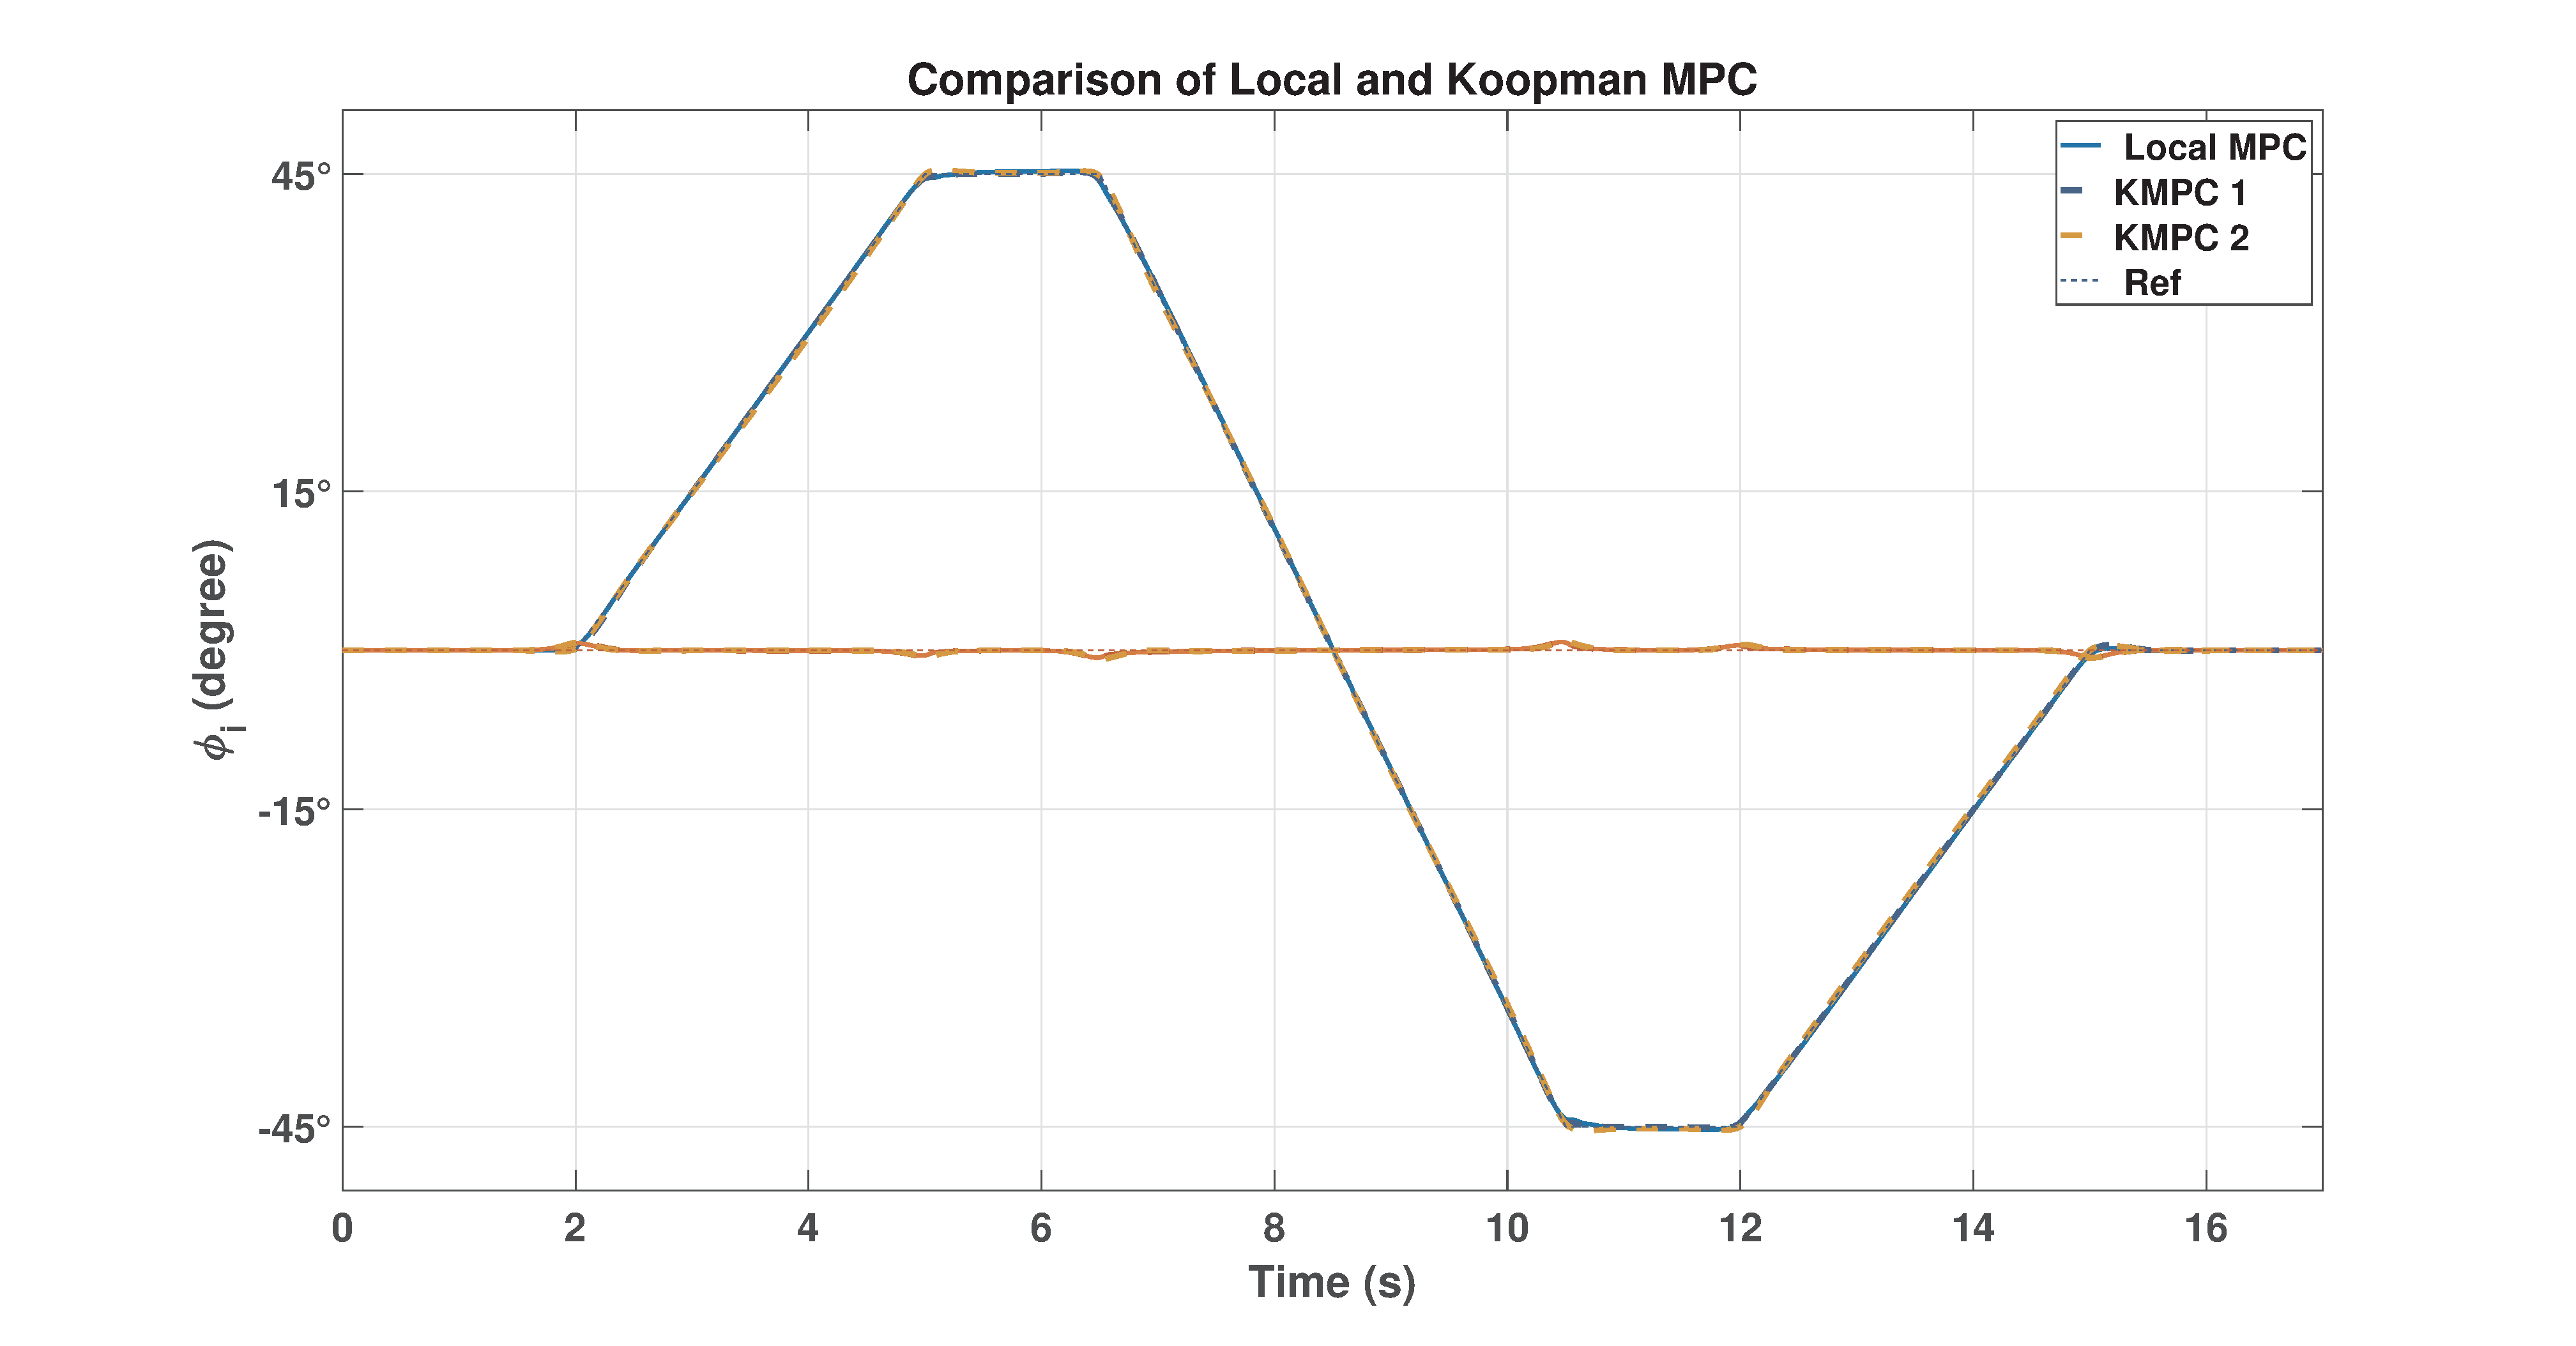
\includegraphics[width=1\linewidth]{figures/LocalKMPC12_5ms}
    \caption{Comparison of Local MPC, Koopman MPC for $\mathbf{\Psi_1}$ (KMPC1) and $\mathbf{\Psi}_4$} (KMPC2)
    \label{fig: LocalKMPC12}
\end{figure}
% 
% 
\begin{figure}[H]
    \centering
    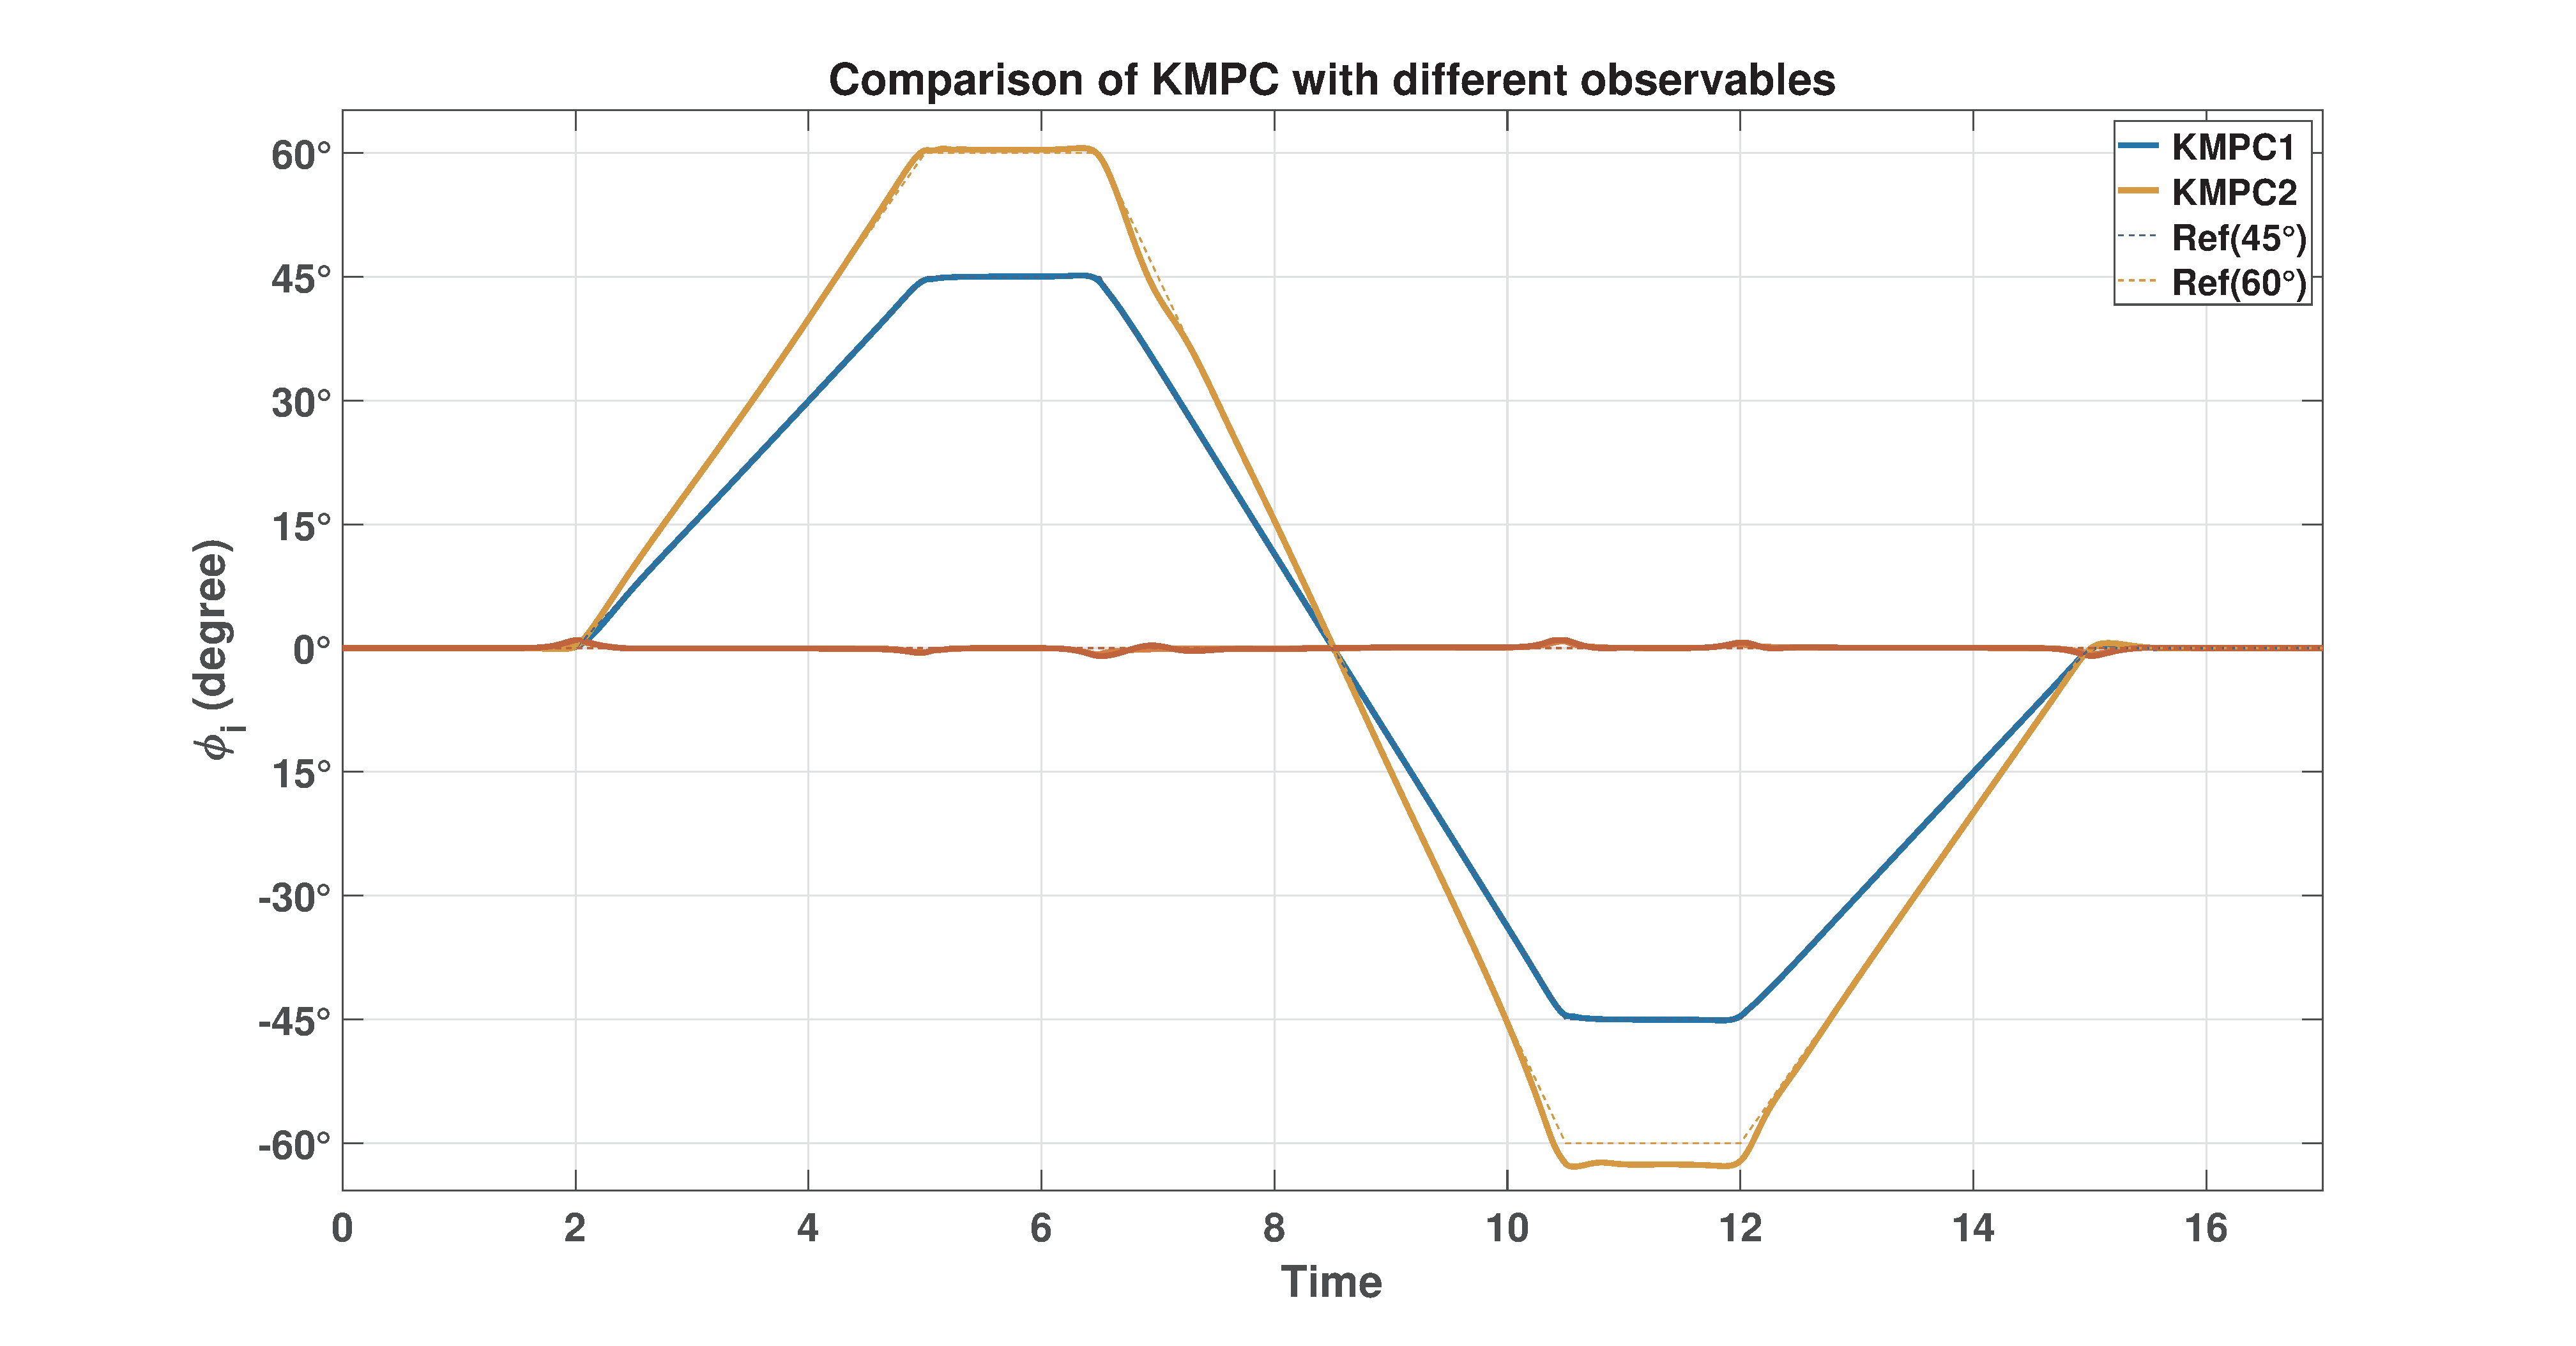
\includegraphics[width=1\linewidth]{figures/KMPC_comp_5ms}
    \caption{Comparison of Koopman MPC for $\mathbf{\Psi_1}$ (KMPC~1) and $\mathbf{\Psi}_4$} (KMPC~2)
    \label{fig: KPMC_comp}
\end{figure}
% 
Table~\ref{tab:Exec} and Table~\ref{tab:RMSE_2} compare the average execution times and relative RMSE for the above presented model-controller combinations, respectively. It can be seen that while the range of tracking could successfully be increased from $45^\circ$ to $60^\circ$ by augmenting the state vector with RBFs, there is no significant increase in the computation time or the relative RMSE (for $45^\circ$ reference trajectory). This is due to the dense formulation of the MPC, as discussed previously. The slight increase in computation time is because one needs to lift the system's state at every computation step. However, the augmented state would have a negligible effect on the computation time of the optimal control input as the matrices $\mathbf{\Bar{A}}$ and $\mathbf{\Bar{B}}$ are pre-computed offline. \par
In the following tables in this section, $\textup{KO}_1$ and $\textup{KO}_2$ are the data-driven models generated by the observables $\mathbf{\Psi}_1$ and $\mathbf{\Psi}_4$, respectively.
\begin{table}[H]
    \centering
    \begin{tabular}{lcc}
         \toprule
                                  & \multicolumn{2}{c}{Average execution time~(ms)}\\
        \cmidrule{2-3}
         Model - Controller       & $T_s = 5$ms  & $T_s = 10$ms\\
         \midrule
         Local - MPC               & 0.56        & 0.17\\
         $\textup{KO}_1$ - MPC    & 0.59         & 0.18\\
         $\textup{KO}_2$ - MPC    & 0.69         & 0.28\\
         \bottomrule
    \end{tabular}
    \caption{Average execution time~(ms) of the MPC algorithms for different sampling times}
    \label{tab:Exec}
\end{table}
% 
\begin{table}[H]
    \centering
    \begin{tabular}{lcc}
         \toprule
                                            & \multicolumn{2}{c}{RMSE(\%)}\\
        \cmidrule{2-3}
         Model - Controller                  & $T_s = 5$ms & $T_s = 10$ms\\
         \midrule
         Local - LQi                         & 6.60       & 7.13\\
         $\textup{KO}_1$ - LQi               & 6.32       & 6.59 \\
         Local - MPC                         & 0.69       & 2.84\\
         $\textup{KO}_1$ - MPC               & 0.53       & 3.53\\
         $\textup{KO}_2$ - MPC - $45^\circ$  & 0.72       & 3.49\\
         $\textup{KO}_2$ - MPC - $60^\circ$  & 2.67       & 2.45\\
         \bottomrule
    \end{tabular}
    \caption{RMSE(\%) of tracking errors for different sampling times}
    \label{tab:RMSE_2}
\end{table}
Next, the robustness of tracking is tested for the synthesized controller. Originally, the controller was synthesized (GA-tuned) for the trajectory shown in Fig.~\ref{fig:ReferenceTraj} where the time to reach the extreme points was $T = 3s$. It is interesting to observe this controller's behaviour on trajectories with steeper slopes, for example, with $T = 1.5s$ and $T = 1s$. Table~\ref{tab:RMSE_diffslopes} presents the results of such a comparison. The values shown in red correspond to the percentage increase in the relative RMSE to the relative RMSE of the model-controller combinations for the original reference trajectory, presented in the first column. It must be noted that from here on, the comparisons are made for data-driven models approximated with data sampled at 5ms. The reason 5ms was selected is that the computation times (Table~\ref{tab:Exec}) are well within the hardware capabilities of the computer and the relative RMSE (Table~\ref{tab:RMSE_2}) for $T_s = 5$ms is much lesser in all the cases when compared to $T_s = 10$ms, making the sampling time of 5ms an obvious choice.
\begin{table}[H]
    \centering
    \begin{tabular}{llll}
         \toprule
                                            & \multicolumn{3}{c}{RMSE(\%)}\\
        \cmidrule{2-4}
         Model - Controller                  & $T = 3$s & $T = 1.5$s & $T = 1$s \\
         \midrule
         Local - LQi                         & 7.13       & 10.03~(\textcolor{red}{+40.7\%})      & 13.35~(\textcolor{red}{+87.2\%})\\
         $\textup{KO}_1$ - LQi               & 6.59       & 9.26~(\textcolor{red}{+40.5\%})       & 12.55~(\textcolor{red}{+90.4\%})\\
         Local - MPC                         & 0.69       & 0.94~(\textcolor{red}{+36.2\%})       & 1.26~(\textcolor{red}{+82.6\%})\\
         $\textup{KO}_1$ - MPC               & 0.53       & 0.85~(\textcolor{red}{+60.3\%})       & 1.29~(\textcolor{red}{+143.4\%})\\
         $\textup{KO}_2$ - MPC - $45^\circ$  & 0.72       & 0.86~(\textcolor{red}{+19.4\%})       & 1.58~(\textcolor{red}{+119.4\%})\\
         $\textup{KO}_2$ - MPC               & 2.67       & 2.87~(\textcolor{red}{-})       & 2.67~(\textcolor{red}{-})\\
         \bottomrule
    \end{tabular}
    \caption{RMSE(\%) of tracking errors for different target times $T$}
    \label{tab:RMSE_diffslopes}
\end{table}
A few observations are in order. 
\begin{itemize}
    \item Firstly, consider the first two rows; it can be seen that the percentage increase in the relative RMSE for the local model and Koopman model $\textup{KO}_1$ is comparable, which means that the recorded data captured most of the dynamics of the underlying nonlinear dynamical system. This consequently validates the approach employed in Section~\ref{sec:Results_ident} to record the data and highlights the effectiveness of the data-driven regression methods described in Chapter~\ref{Chapter:Prelims}.
    \item Next, comparing rows 1 and 3 it can be seen that the MPC controller performs slightly better compared to the LQi, which is of course expected. Also, note that the relative RMSE was significantly lower for the MPC controller to start with.
    \item The comparison of rows 4 and 5 shows that the model with state vector augmented with RBFs seems to capture relatively more relevant dynamics than just the state vector as observables, and consequently, the relative increase in the RMSE for varying slopes is much lesser, i.e., the model-controller combination, ($\textup{KO}_2 - \textup{MPC}$), seems to track the various trajectories much closer than the $\textup{KO}_1 - \textup{MPC}$ combination.
    \item It is seen that the result of comparison between row 2 and row 4, LQi and MPC controller applied to the $\textup{KO}_1$ model, respectively, is not as expected. The MPC controller performs relatively worse than an LQi controller. A possible explanation for this could not be ascertained. It could only be guessed that the $\textup{KO}_1-\textup{MPC}$ combination has the lowest relative RMSE of all the combinations for $T = 3s$, and a small but reasonable increase in the RMSE contributes much more than compared to the same in the case of KLQi.
    \item The last row presents some important insight into the choice of observables.\\Figure~\ref{fig: cont_traj} visualizes the results of the last row. It can be seen that as the slope becomes steeper, the tracking range of the model-controller combination decreases. A potential explanation to this could be that the choice of observables, while good, may not be the best, and there may exist some other combination of RBFs which perform better. This is left to further research. It can also be construed as a possible limitation of data-driven models, and that these models may not perform as well as a model derived from first principles. This can be seen in the following results. 
\end{itemize}
% 
\begin{figure}[H]
    \centering
    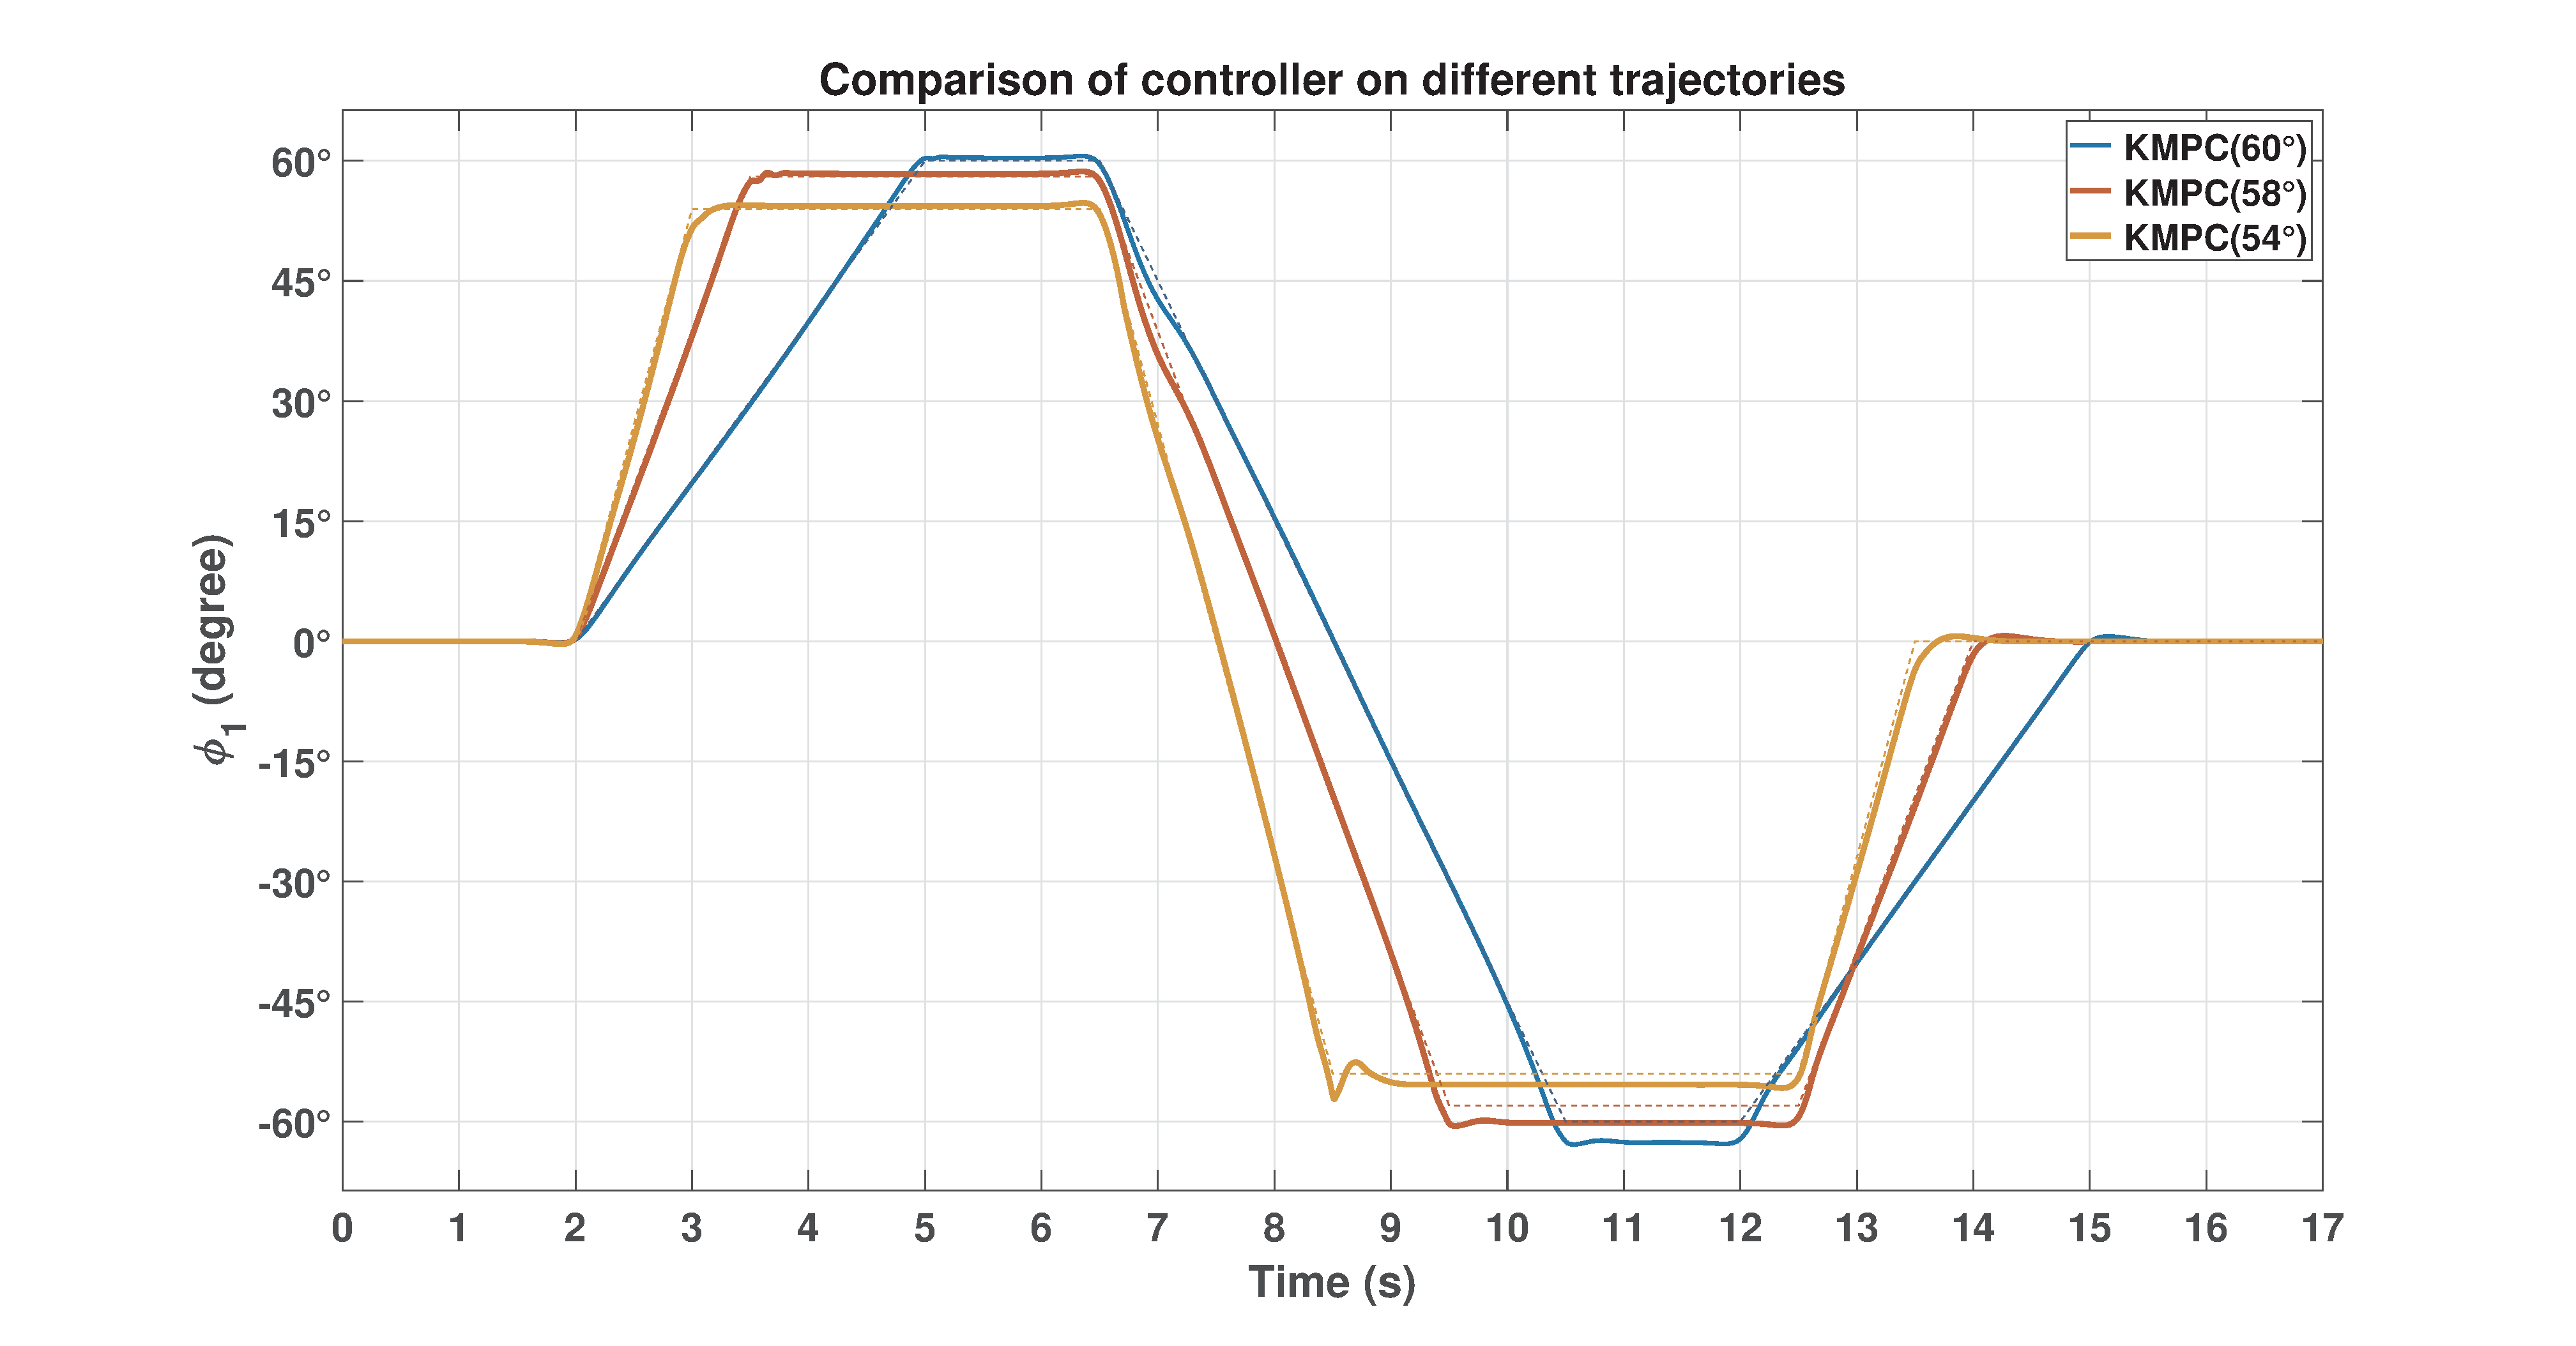
\includegraphics[width=1\linewidth]{figures/Cont_diffTraj}
    \caption{Comparison of the synthesized controller on reference trajectories with different degrees of slopes for Koopman model approximated using $\mathbf{\Psi}_4$. (\textcolor{blue}{\textbf{--}}) -- $T = 3s$,(\textcolor{red}{\textbf{--}}) -- $T = 1.5s$, and (\textcolor{orange}{\textbf{--}}) -- $T = 1s$}
    \label{fig: cont_traj}
\end{figure}
% 
Consider a quasi-linear parameter varying~(qLPV) model of the ADIP parameterized with scheduling parameters $\rho = [\phi_1 \quad \Dot{\phi}_1]$ as described by Cisneros et al. \cite{qLMPC}. A corresponding MPC controller is synthesized for this model, tuned by a GA. The tuning parameters are $\mathbf{Q} = \textup{diag}(1884.43,~1777.43,~80.16,~0.76)$ and $\textup{R} = 26.13$ and $\mathbf{Q}_N = 2219.42\mathbf{Q}$.\par
It is important to note that the prediction horizon for the qLPV-MPC (here-on, qLMPC) is taken as $N_p = 40$, as against $N_p = 200$, which was the prediction horizon considered previously. The reason to choose a lower prediction horizon in the case of qLMPC is that, at every time step, a linear model is computed for which a new MPC is synthesized which then returns the optimal control input for the next time step and this process is repeated. This is a computationally costly process, and the computation cost further increases exponentially with the increase in the prediction horizon. Table~\ref{tab:Exec_predHor} illustrates this. 
\begin{table}[H]
    \centering
    \begin{tabular}{lcc}
         \toprule
                                  & \multicolumn{2}{c}{Average execution time~(ms) for $T_s$ = 5ms}\\
        \cmidrule{2-3}
         Model - Controller       & $N_p = 200$  & $N_p = 40$\\
         \midrule
         Local - MPC               & 0.56        & 0.05\\
         $\textup{KO}_1$ - MPC    & 0.59         & 0.06\\
         $\textup{KO}_2$ - MPC    & 0.69         & 0.16\\
         $\textup{qLPMC}$         & 10.2         & 0.40\\
         \bottomrule
    \end{tabular}
    \caption{Average execution time~(ms) of the MPC algorithms for different prediction horizons}
    \label{tab:Exec_predHor}
\end{table}
It can be seen that for a prediction horizon of $N_p = 200$, the computation time is more than 10ms for the qLMPC, whereas it is 0.40ms for a prediction horizon of $N_p = 40.$ Moreover, the results obtained with $N_p = 40$ can be considered good enough, and there is actually no need to increase the prediction horizon further. In previously considered models, however, the possibility of a longer prediction horizon enables better results. One can use the prediction horizon of $N_p = 200$, simply because the computational cost is well within the hardware requirements. The corresponding results are quite good. The average execution time of the MPC for the local model and data-driven model is significantly low even with a prediction horizon of $N_p = 200$ because the MPC here is based on a linear model whose matrices are pre-computed offline as against online computation of the linear matrices in the case of qLMPC. \par
Figure~\ref{fig: cont_traj_qLMPC} presents a qLMPC version of the comparison made previously in Fig.~\ref{fig: cont_traj}. 
% 
\begin{figure}[H]
    \centering
    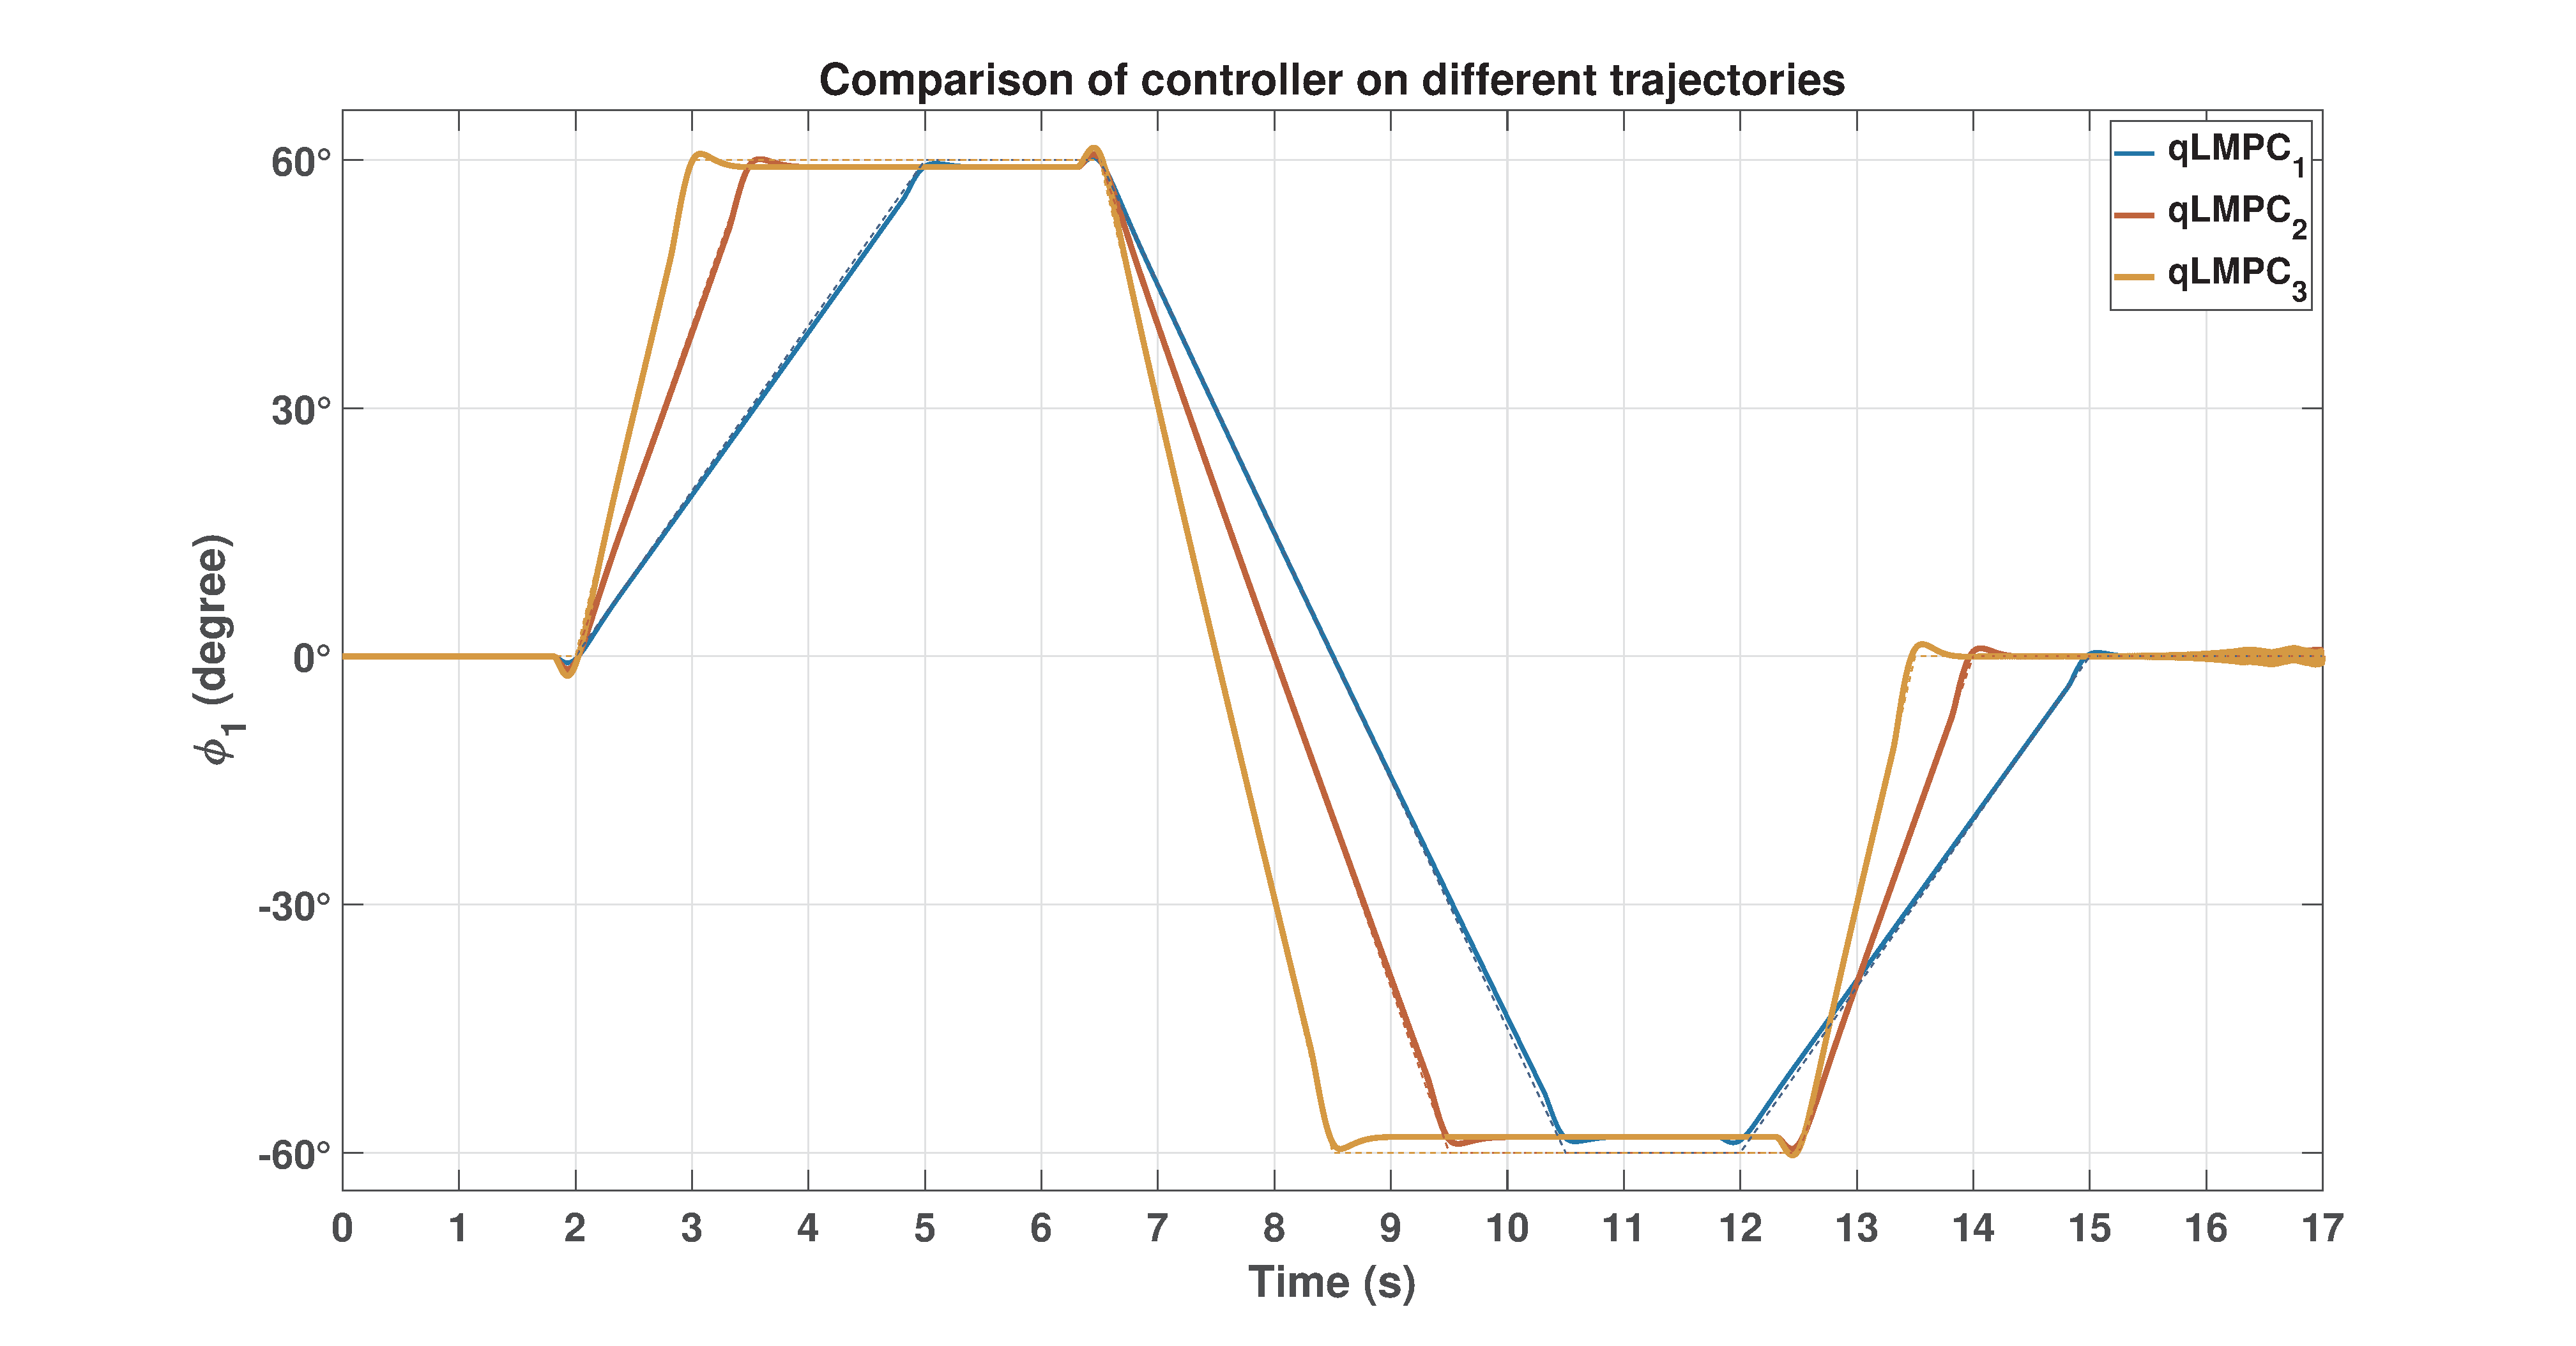
\includegraphics[width=1\linewidth]{figures/qLMPC_comp}
    \caption{Comparison of the synthesized qLMPC controller on reference trajectories with different degrees of slopes. (\textcolor{blue}{\textbf{--}}) -- $T = 3s$,(\textcolor{red}{\textbf{--}}) -- $T = 1.5s$, and (\textcolor{orange}{\textbf{--}}) -- $T = 1s$}
    \label{fig: cont_traj_qLMPC}
\end{figure}
% 
The corresponding relative RMSE values are presented in Table~\ref{tab:RMSE_diffslopes_qlmpc}.
\begin{table}[H]
    \centering
    \begin{tabular}{lccc}
         \toprule
                                            & \multicolumn{3}{c}{RMSE(\%)}\\
        \cmidrule{2-4}
         Model - Controller                  & $T = 3$s & $T = 1.5$s & $T = 1$s \\
         \midrule
         qLPV - MPC                         & 2.15       & 2.24     & 2.43\\
         \bottomrule
    \end{tabular}
    \caption{RMSE(\%) of tracking errors for different target times}
    \label{tab:RMSE_diffslopes_qlmpc}
\end{table}
% 
An important observation can be made from Fig.~\ref{fig: cont_traj_qLMPC} and Table~\ref{tab:RMSE_diffslopes_qlmpc}; the relative RMSE does not increase significantly with change in the slope of the reference trajectory, and also, the RMSE for qLMPC is lesser than that of a data-driven model with MPC approximated with $\mathbf{\Psi}_4$. Furthermore, the qLMPC can track up to $60^\circ$ for all the degrees of slope considered whereas, the $\textup{KO}_2-\textup{MPC}$ failed to track the desired target for steeper slopes of the reference trajectory. This points out a key limitation of data-driven models. A data-driven model might work better than a locally linearized first-principles model in the region where training data is captured, but it is possible that the data models may not perform on par with a quasi-linear parameter varying model. With the increase in computational capabilities, the qLPV approach seems much more promising. Nevertheless, one must note that an important assumption made here is the availability of a mathematical model of the system. Without this, the qLPV approach is not possible and the data-driven model stands as the obvious choice. \par
During the course of implementation, two additional important observations were made. First, although the Koopman approximated system is a linear representation of the underlying nonlinear dynamics, and in theory one can use any of the model-based linear control techniques to control the system, it is highly recommended to use a predictive controller like the MPC rather than a non-predictive controller like LQi for tracking tasks. This is because the extended state of observables more often than not contains nonlinear functions of the state. The LQi which computes the cost over the infinite horizon fails to solve the optimal control problem. It requires careful handpicking of observables to overcome this. Whereas, since the MPC predicts only over a reasonably small time horizon, it is often easier to manage any irregularities caused by nonlinear observables' evolution. Therefore, when working with data-driven models, MPC is a better choice than non-predictive controllers.\par
Second, as an additional exercise, the possibility of identifying and controlling a highly unstable system like the ADIP itself in the absence of an optimal controller was explored. At the beginning of this chapter, it was assumed that a plant model was already available. Therefore, an optimal controller, such as the linear quadratic regulator could be synthesized. A Koopman approximated linear system could then be modelled and controlled from just the measured closed-loop data. In the absence of such a controller, one may synthesize a non-model based PID controller that may not have the optimal tuning parameters for it to cover the necessary range of the desired trajectory. It was observed that it is possible to extend this range by recursively applying the EDMD approximation on the obtained data to generate a new linear model at every step for which a powerful model-based controller could be designed and consequently extend the range.\par
As an example, assume that the measurement data could be recorded for only $5^\circ$ from the up-up configuration after which the controller fails to track, as opposed to data recorded for a range of $40^\circ$ with an LQi controller(as shown in Fig \ref{fig:ReferenceTraj}). DMD could then be applied to such data to generate a linear model. With a linear model's availability, one could synthesize a model-based linear controller like the LQi or MPC. It is also possible to generate GA optimized tuning parameters for maximum reach. In this particular case, the range of tracking could be extended by an additional $10^\circ$ with an MPC's help and with the original measured state as the observable vector. Data was then recorded from this new system with a range of $15^\circ$, and the same process was applied to extend the range at each step. Finally, it was observed that the closed-loop tracking performance of the model-controller($\textup{KO}_3$-MPC) combination so obtained was comparable to that obtained from original data with the observable vector $\mathbf{\Psi}_1$. Figure~\ref{fig:diffdata} and Table \ref{tab:RMSE_3} illustrate the tracking performance of such a model with the same controller as used previously with other models. The results can be significantly improved with a controller specifically tuned for this model. However, it failed to perform as well with the $\mathbf{\Psi}_4$, i.e., with the observable vector containing the state and previously defined thin-plate spline RBFs. A potential reason for this might be the RBFs' choice, and there could be some combination of RBFs that may result in better performance. This is left to future research.
% 
\begin{figure}[H]
    \centering
    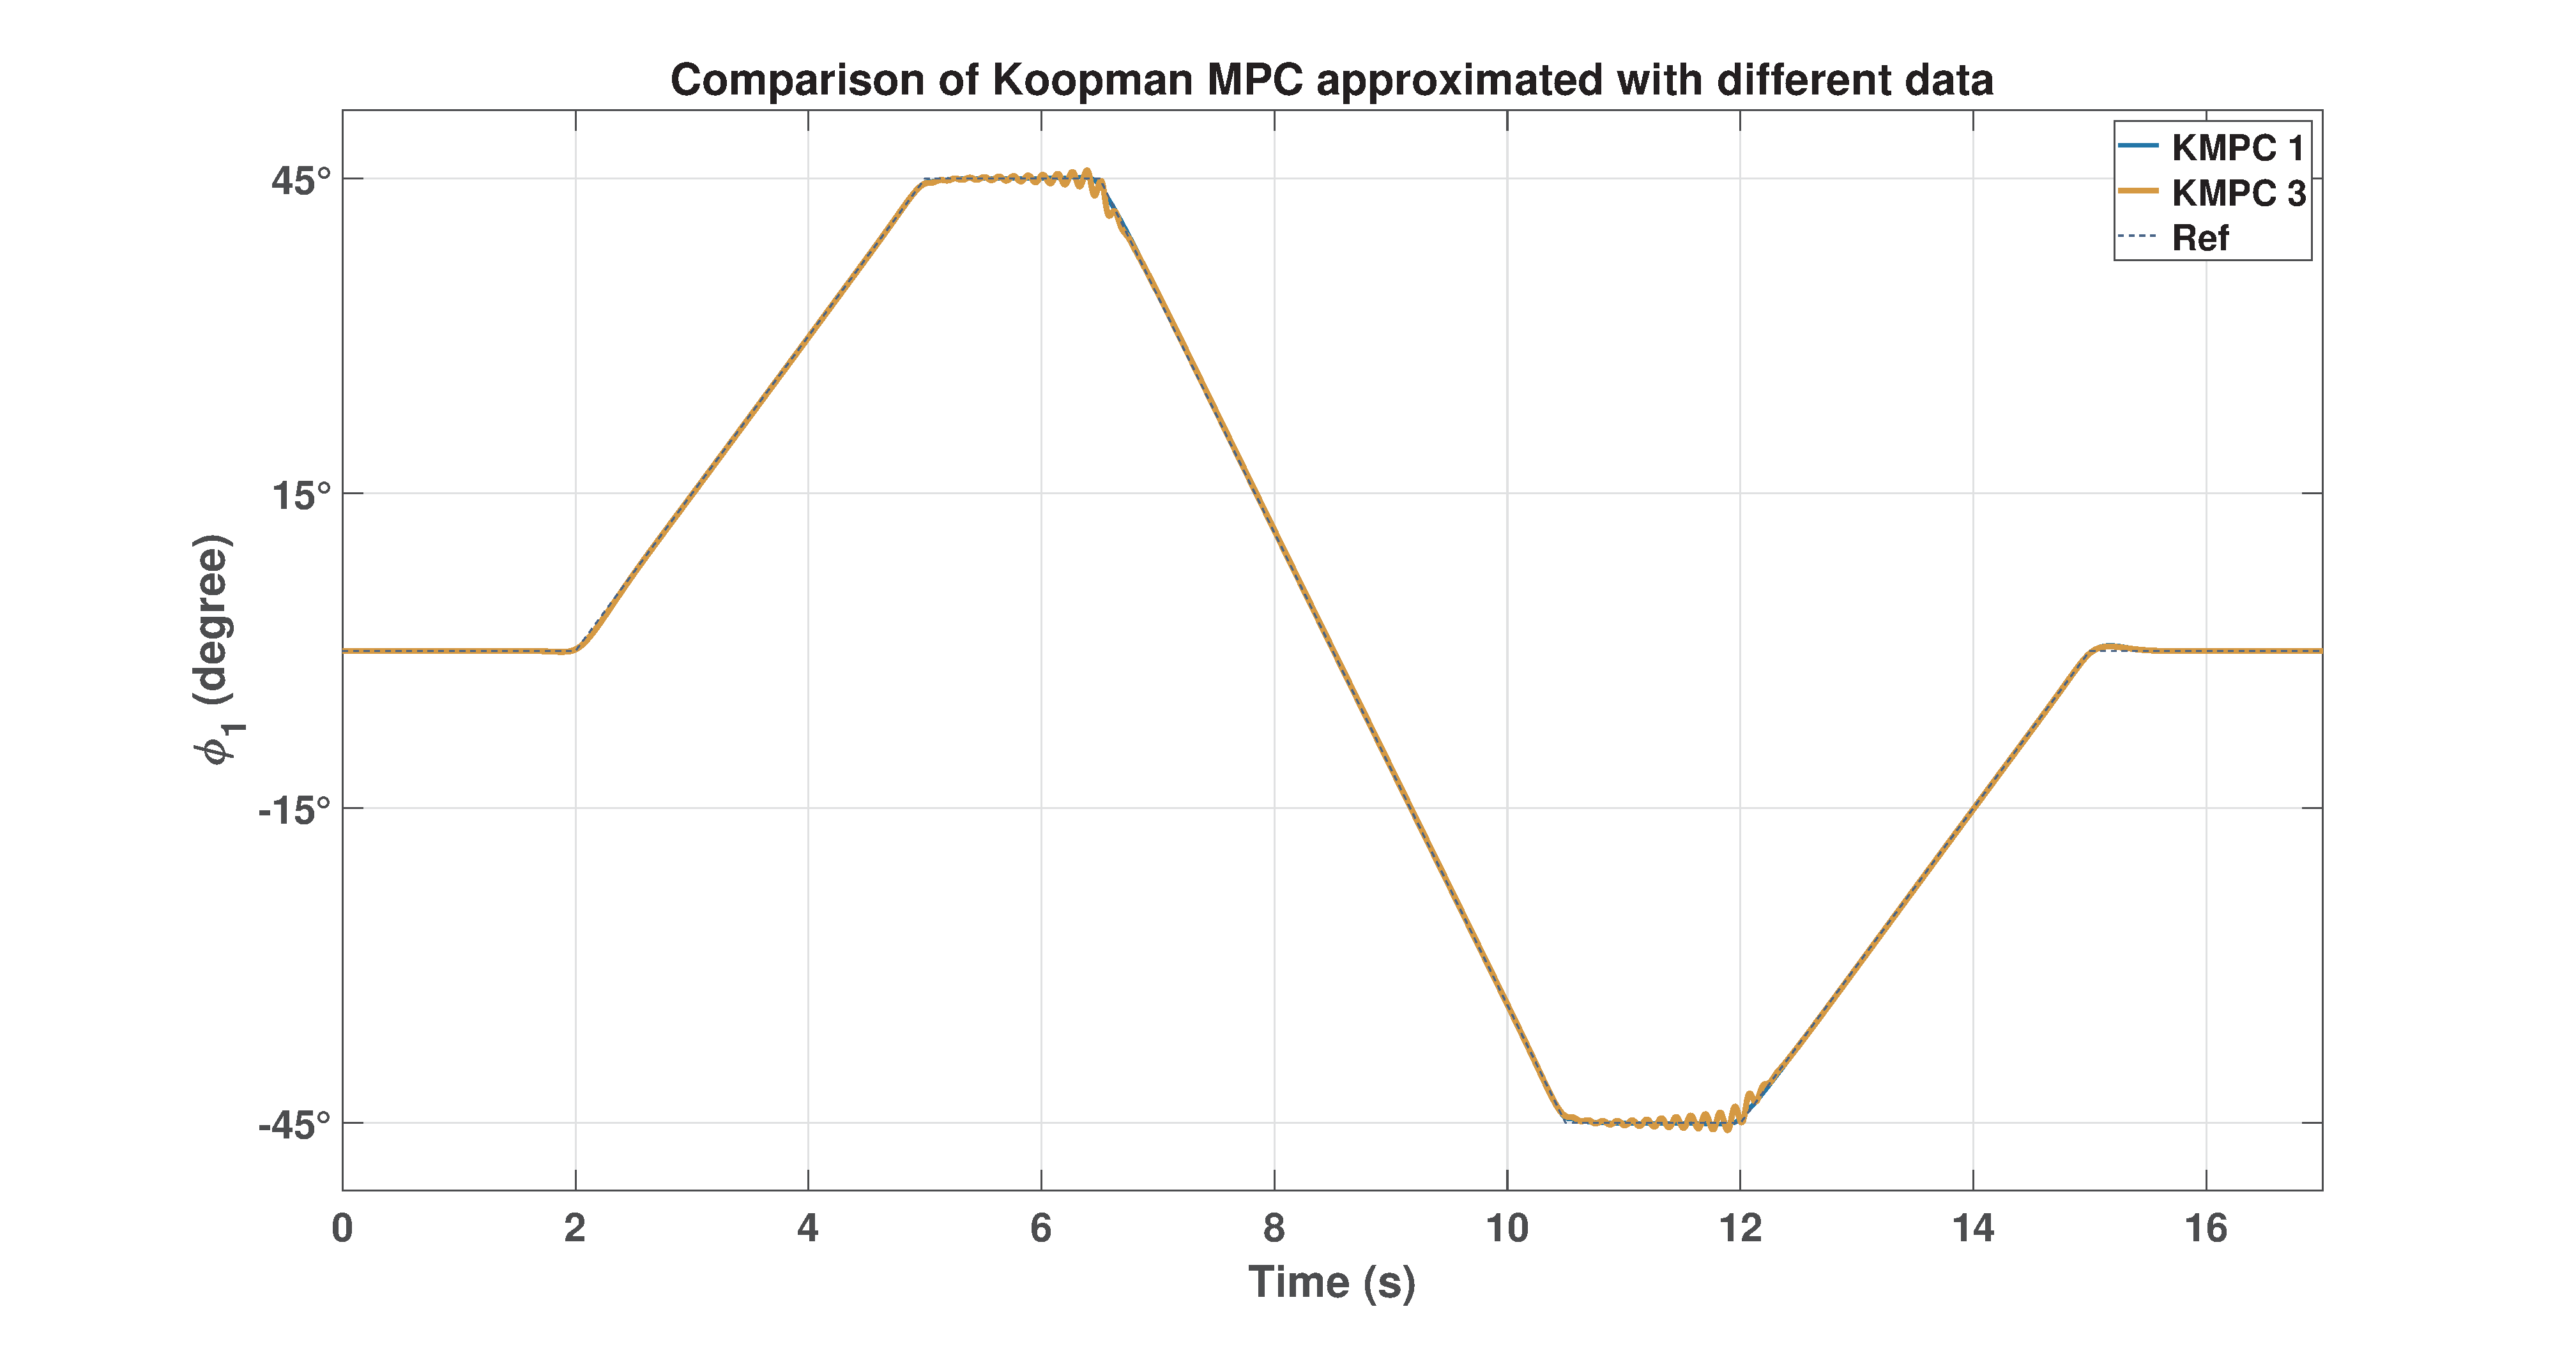
\includegraphics[width=1\linewidth]{figures/KMPC_diffdata}
    \caption{Comparison of Koopman MPC on data-driven model generated with data over a range of upto $40^\circ$ ($\textup{KO}_1$) versus data-driven model ($\textup{KO}_3$) constructed recursively with data generated over a range of upto $5^\circ$}
    \label{fig:diffdata}
\end{figure}
% 
% 
\vspace{-0.5cm}
\begin{table}[H]
    \centering
    \begin{tabular}{lc}
         \toprule
         Model - Controller                  & $T_s = 5$ms\\
         \midrule
         $\textup{KO}_1$ - MPC               & 0.53\\
         $\textup{KO}_3$ - MPC               & 0.95\\
         \bottomrule
    \end{tabular}
    \caption{RMSE(\%) of tracking errors for ($\textup{KO}_1$) and ($\textup{KO}_3$)}
    \label{tab:RMSE_3}
\end{table}
\vspace{-0.5cm}
It is important to reiterate two important assumptions made during the course of this implementation. First, the reference trajectories are fixed and are assumed to be known \textit{a priori}. This is important because the MPC controllers synthesized during the implementation are supplied with future values of the reference to enable the controller to `see' into the future and anticipate any changes in the trajectory. The controller then acts accordingly. This is different from the normally implemented MPC controllers, where only a current value of the reference is supplied. Figure~\ref{fig:antici} visualises this difference. When the controller is supplied with a reference signal of the next $N_p$ steps, it can anticipate the change in trajectory and respond accordingly. 
% 
\begin{figure}[H]
    \centering
    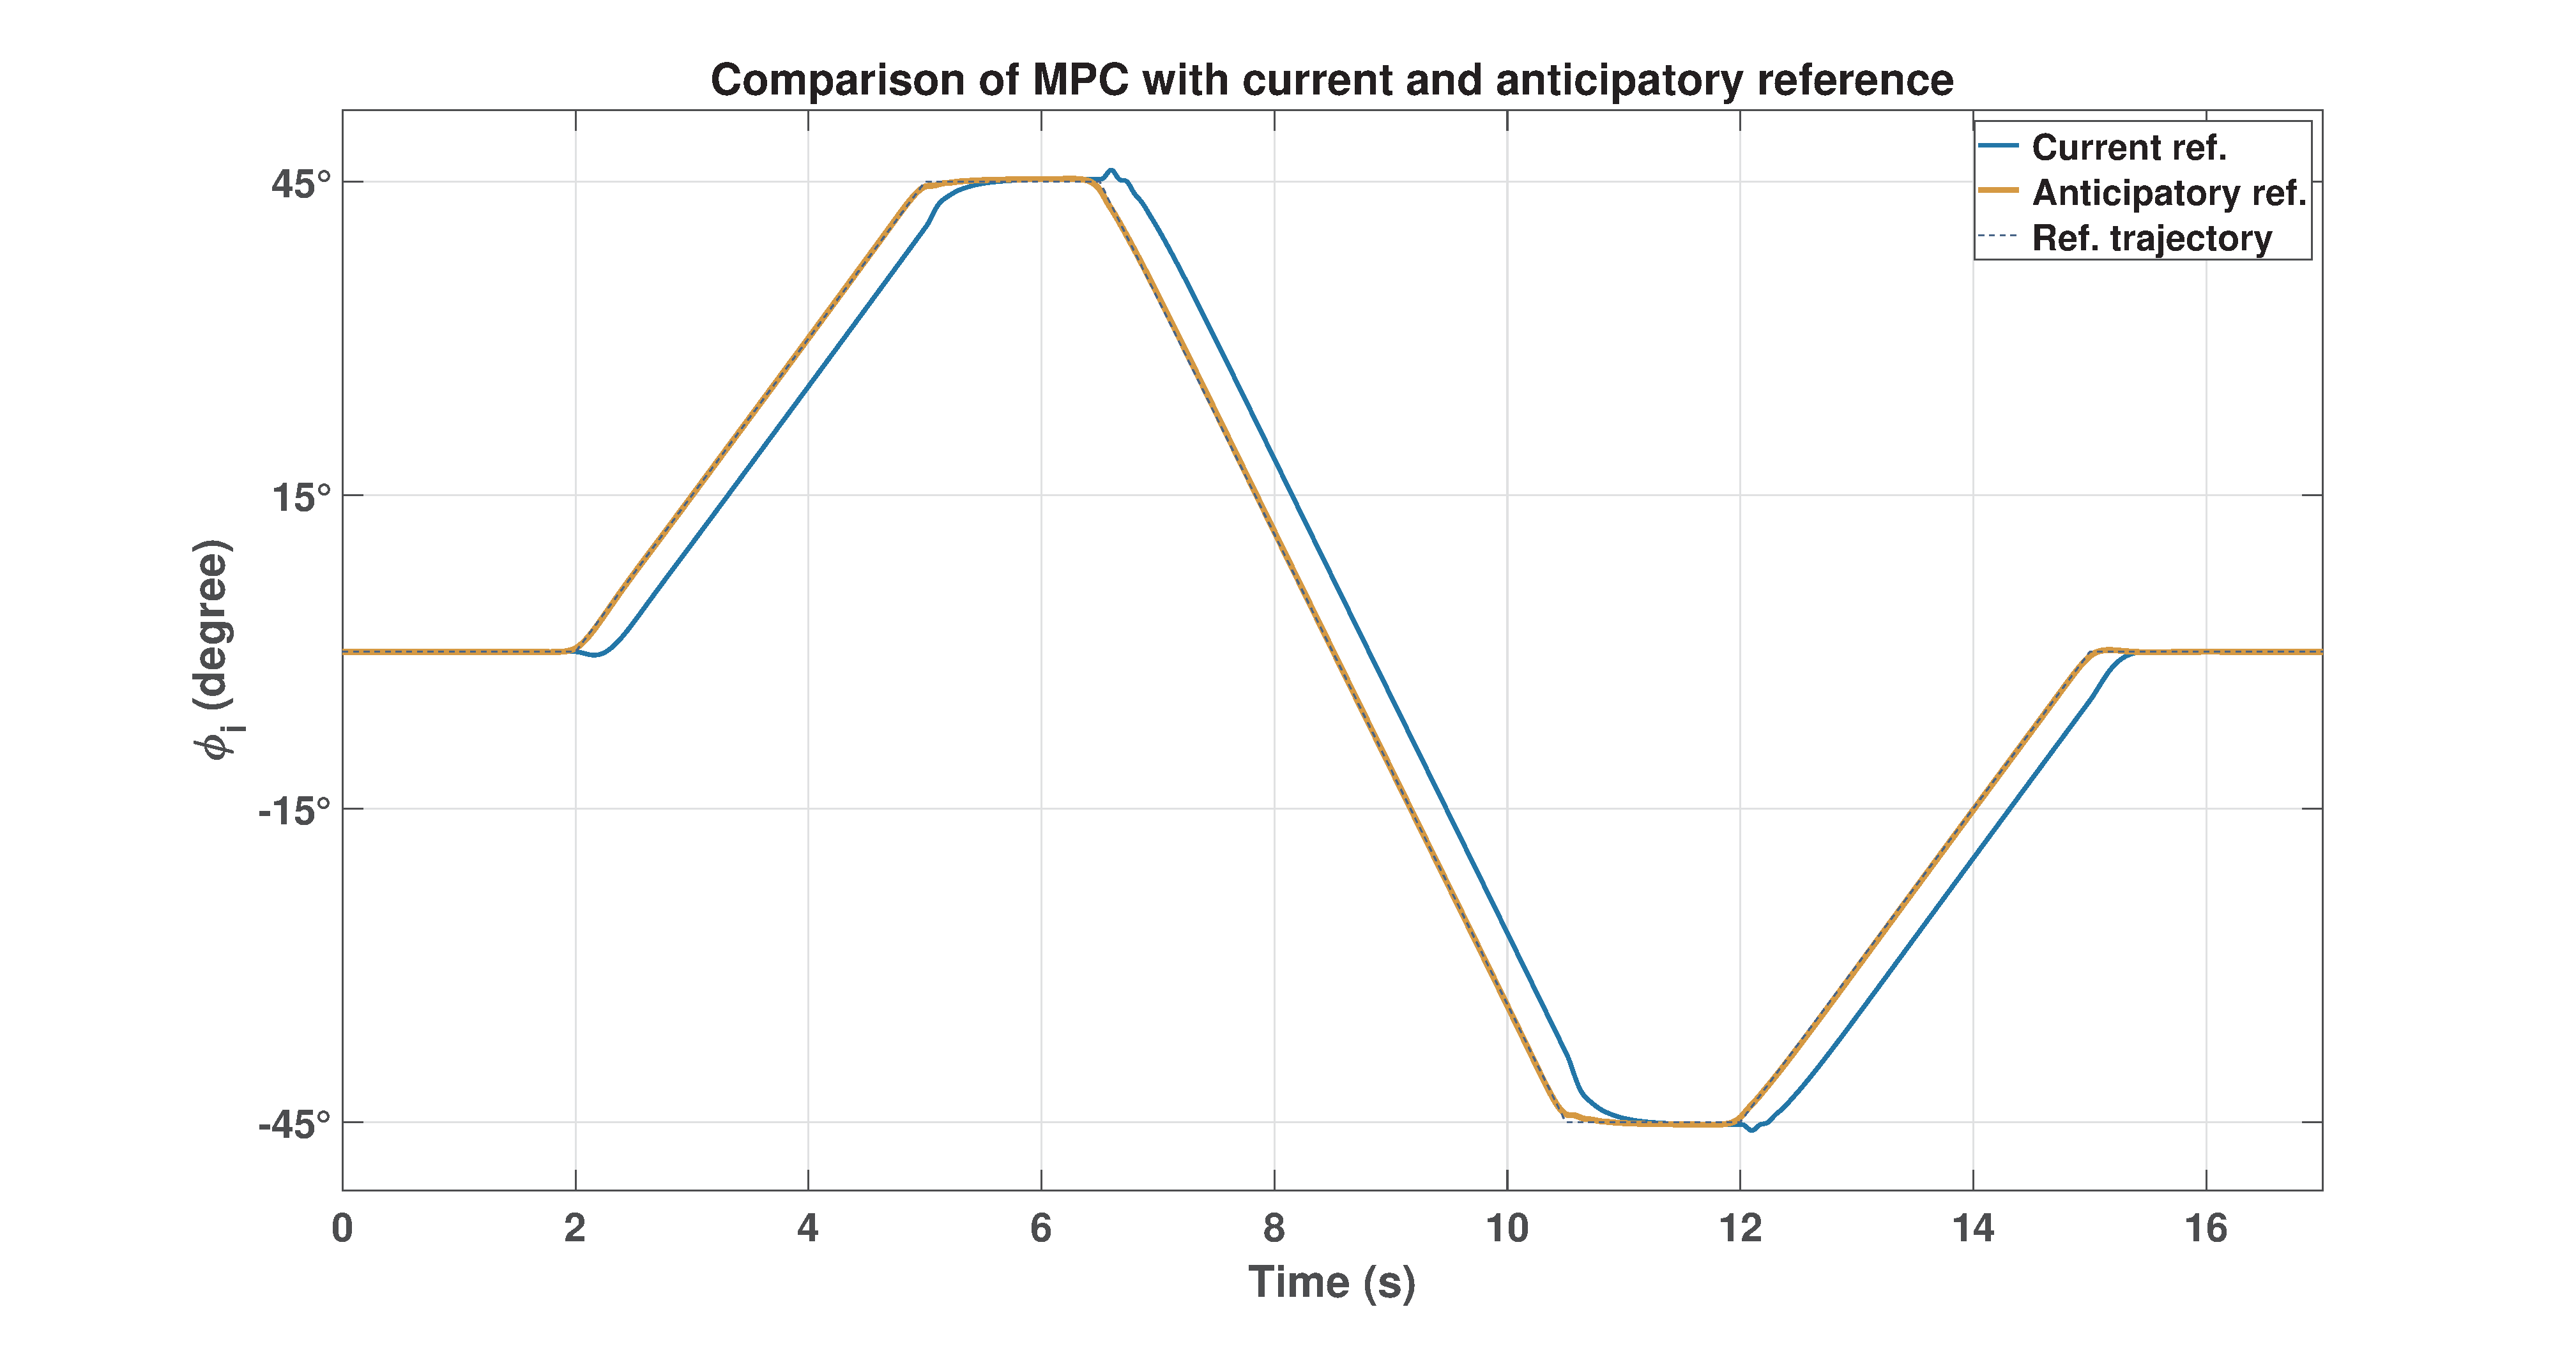
\includegraphics[width=1\linewidth]{figures/anticipatory}
    \caption{Comparison of controller acting on current reference versus anticipatory reference}
    \label{fig:antici}
\end{figure}
% 
\vspace{-0.55cm}
Second, a major assumption made during the genetic algorithm (GA) powered tuning of parameters in this thesis was that it was assumed a nonlinear simulation model of the plant (ADIP) is available to run the GA at all times. This may not always be the case, especially when dealing with systems where the dynamics are unknown. In such a case, one has to either resort to intuition and knowledge of tuning parameters or estimate a nonlinear black-box model of the unknown plant.
\vspace{-0.20cm}




\subsection{Swing-up}
\label{sec:Results_swingup}
Finally, a comparison of two different strategies for swing-up is presented in this section. Both the swing-up strategies are model-based. The first strategy is an energy-based swing-up law adopted from Fantoni et al.~\cite{Fantoni}. Figure \ref{fig:swing_up} shows the evolution of the arm and pendulum angles from down-down configuration at $\phi_1 = \phi_2 = 180^\circ$ to up-up configuration with $\phi_1 = \phi_2 = 0^\circ.$ The approach presented in \cite{Fantoni} ensures that the arm swings up and brings the pendulum into a homoclinic orbit where a stabilizing controller takes over from the energy-based controller and thereafter performs a regulation task to the up-up configuration. The parameters were tuned by a GA which resulted in $k_E = 4.55 $, $k_P = 0.4$, and $k_D = 0.8$. Similarly, Figure~\ref{fig:swing_up_qLMPC} shows the evolution of arm and pendulum angles for a swing-up approach based on the previously introduced qLPV-MPC approach. Here, only one controller is sufficient for both swinging up the pendulum and stabilizing it about the up-up configuration. The swing-up parameters were GA tuned; the parameters are $\mathbf{Q} = \textup{diag}(2623,~746.36,~46.65,~0.51))$ and $\textup{R} = 61.4$ and $\mathbf{Q}_N = 427.25\mathbf{Q}$. Furthermore, Figure \ref{fig:Etilda} shows the change in the system's total energy. The energy-based swing-up law performs significantly better than the qLMPC swing-up law. However, the latter has the advantage that it is just a single controller, unlike the former, which requires an additional stabilizing controller. 
% 
\begin{figure}[H]
    \centering
    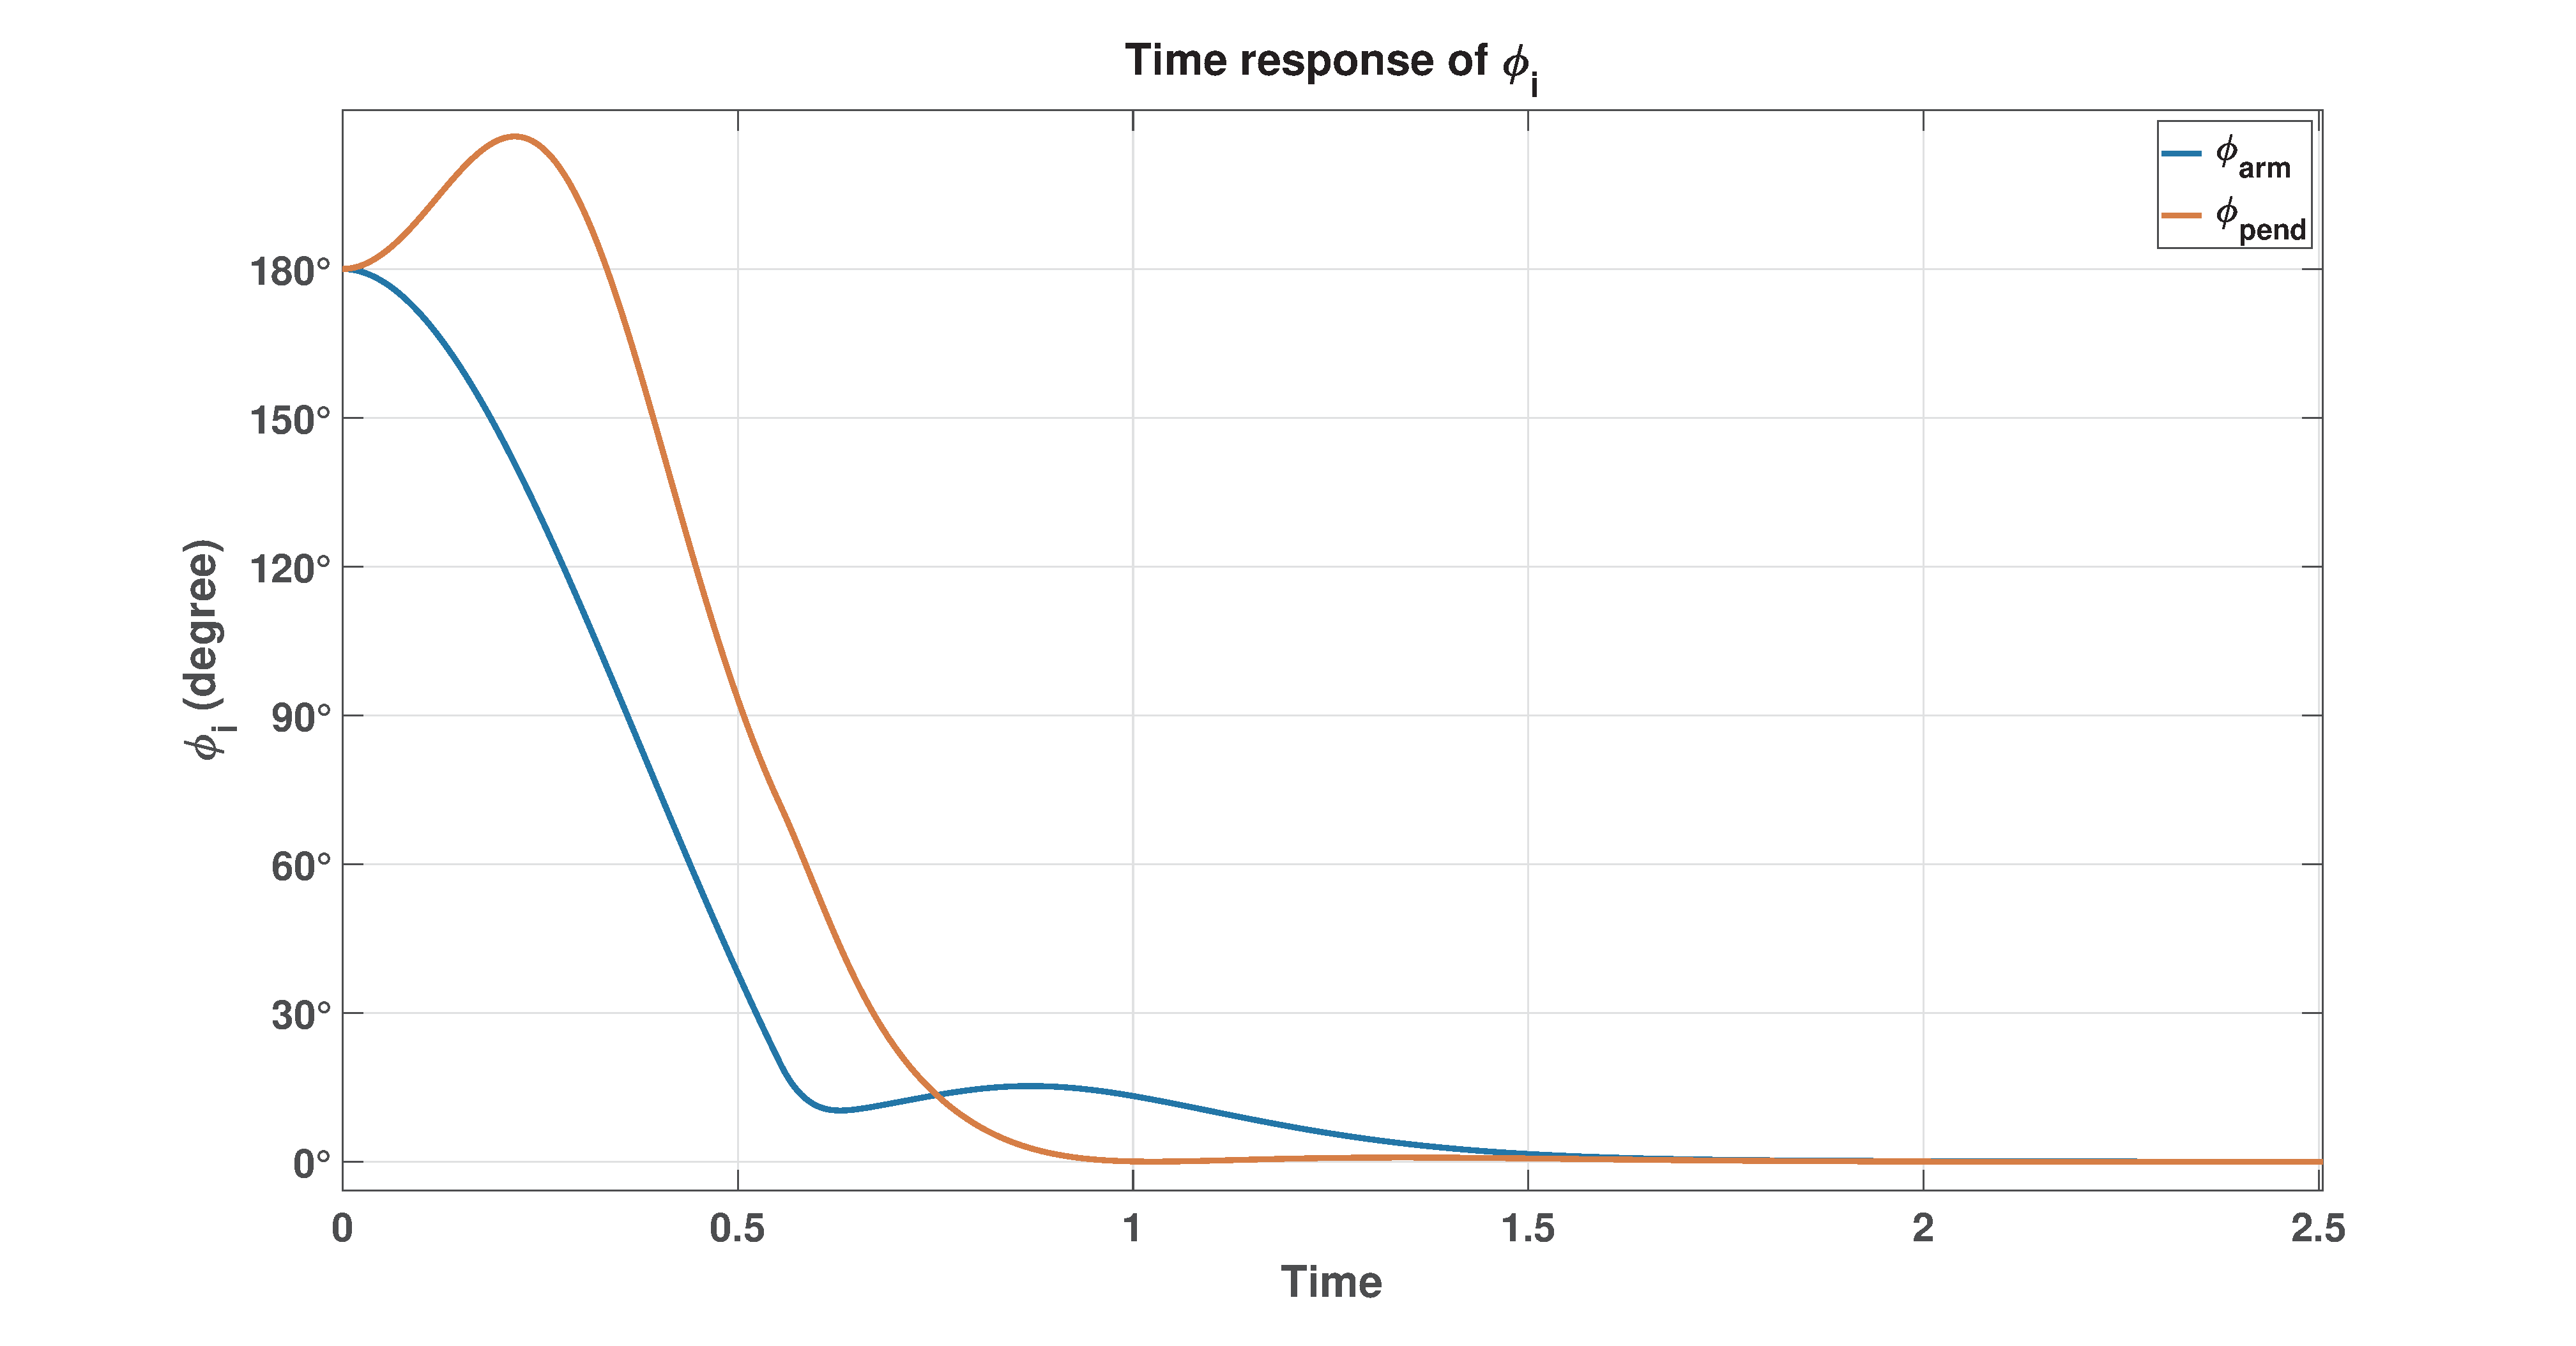
\includegraphics[width=0.84\textwidth]{figures/Swing_up}
    \caption{Swing-up performed by energy-based controller and a stabilizing LQR.}
    \label{fig:swing_up}
% \end{figure}
\vspace{0.004em}
% \begin{figure}[ht]
    \centering
    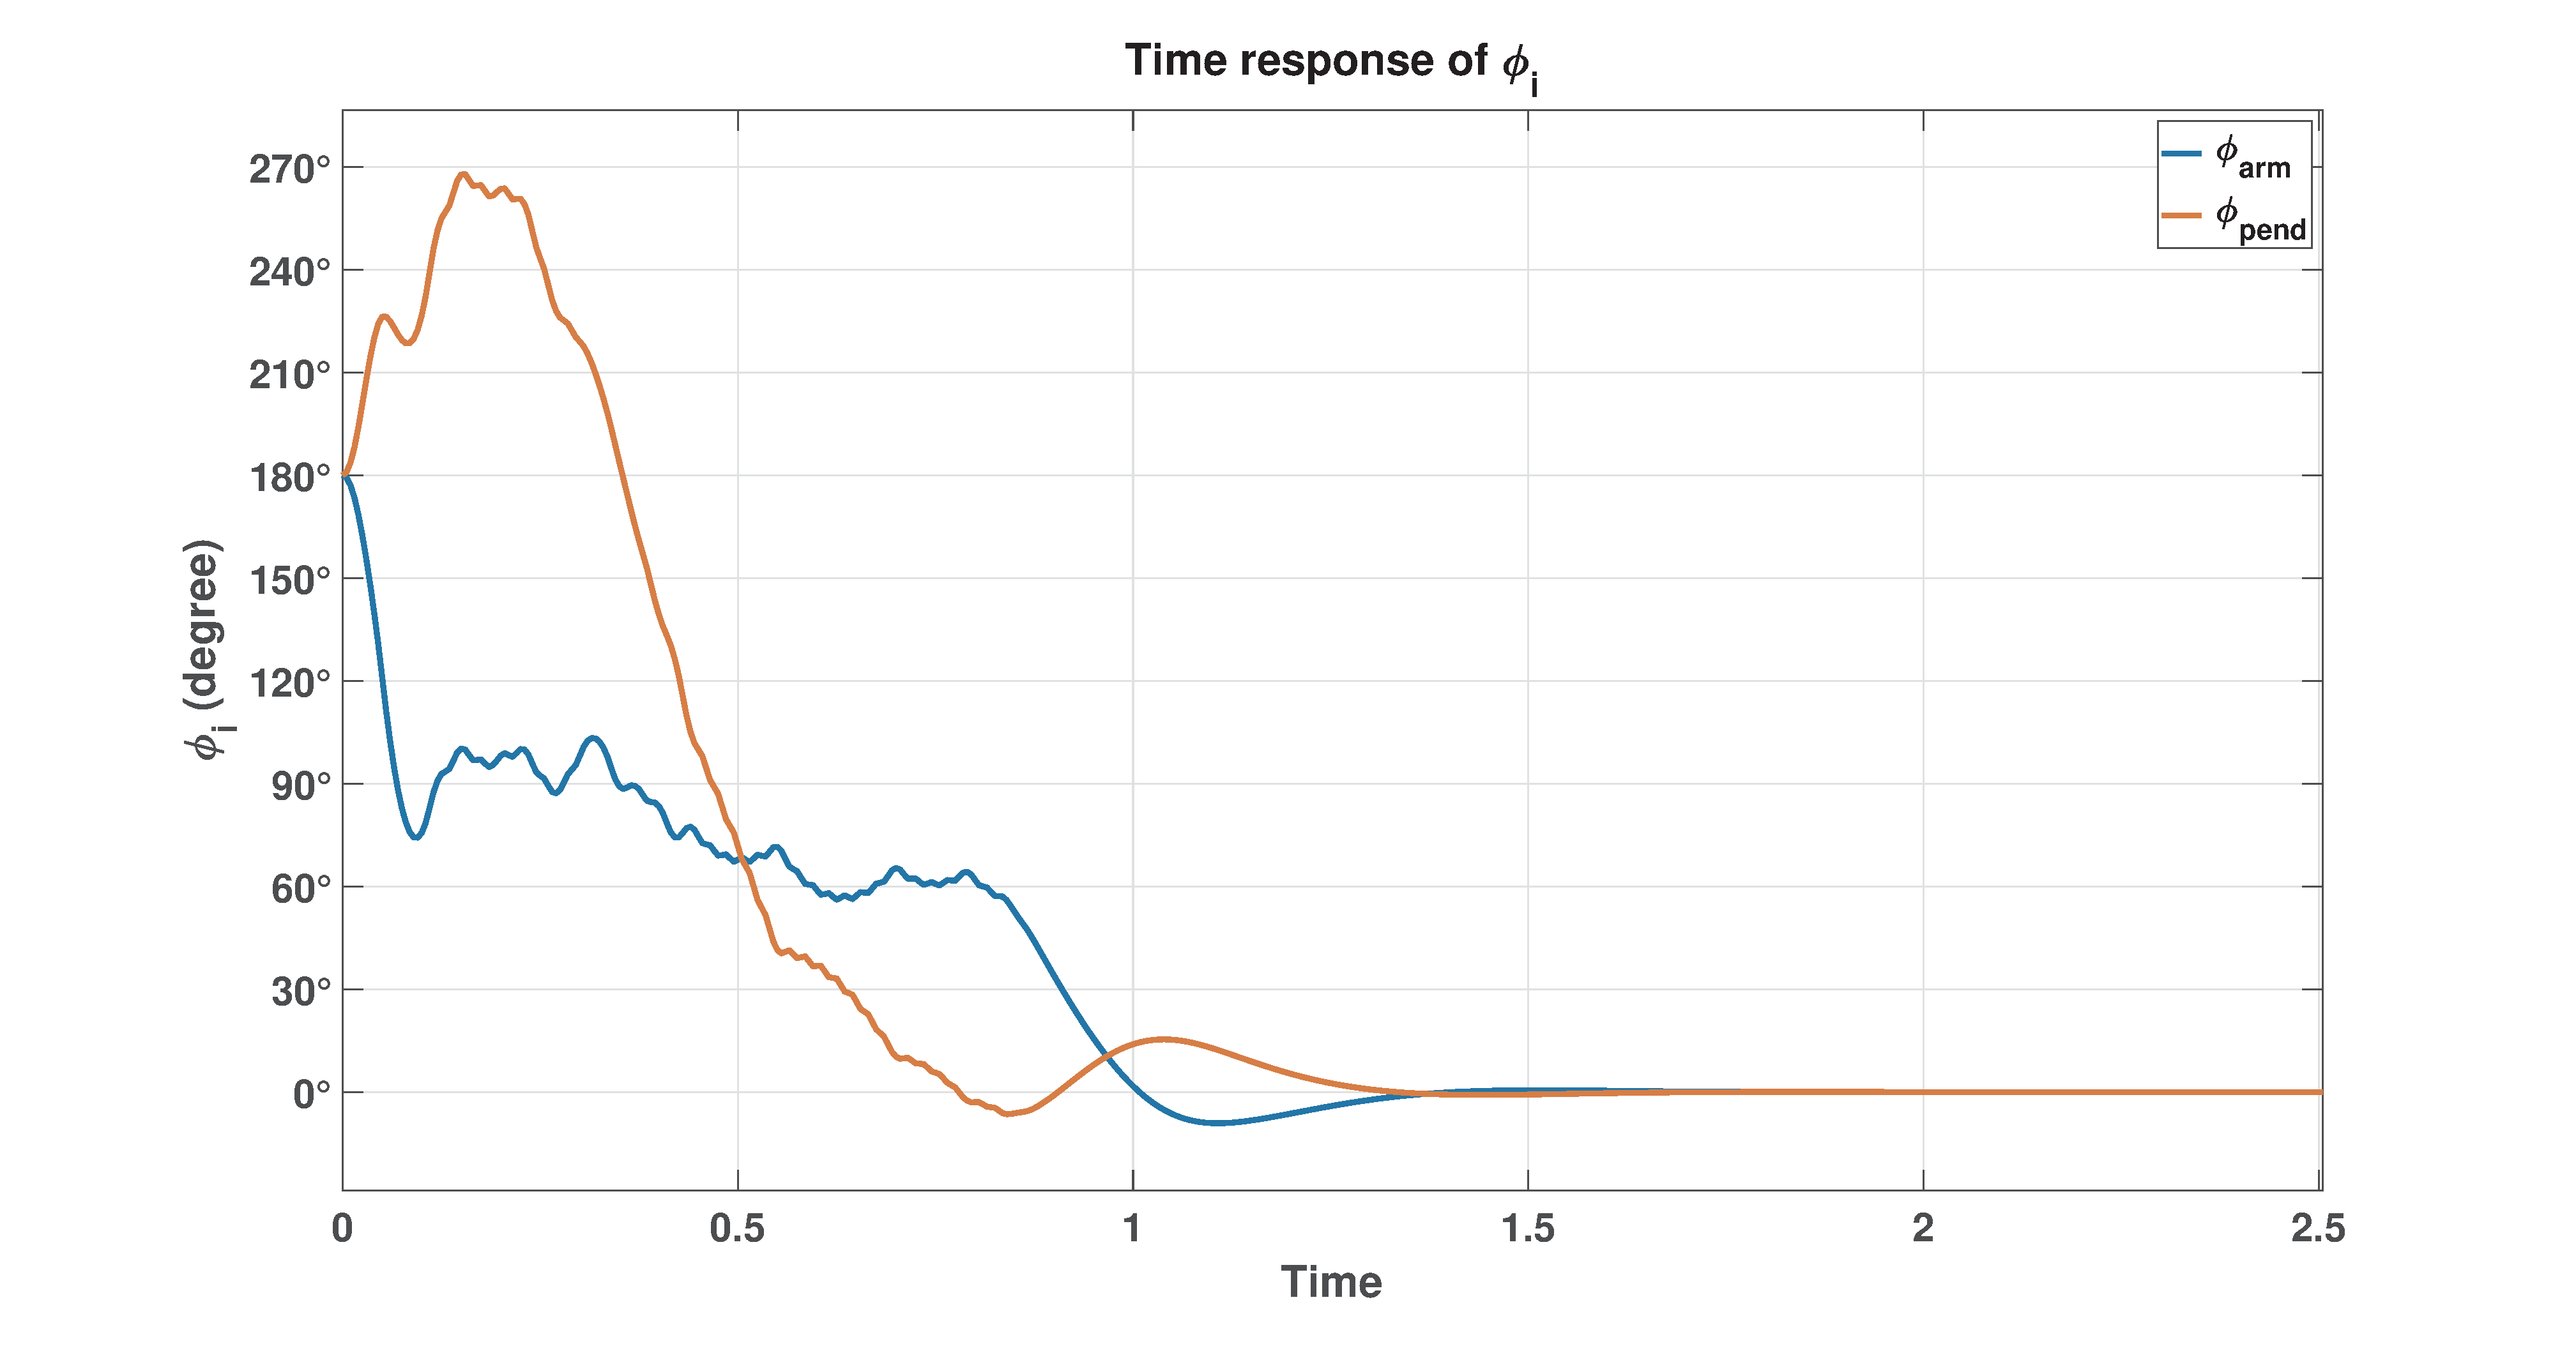
\includegraphics[width=0.84\textwidth]{figures/qLMPC_swingup}
    \caption{Swing-up performed by qLPV-MPC controller}
    \label{fig:swing_up_qLMPC}
% \end{figure}%
\vspace{0.004em}
% \begin{figure}[ht]
    \centering
    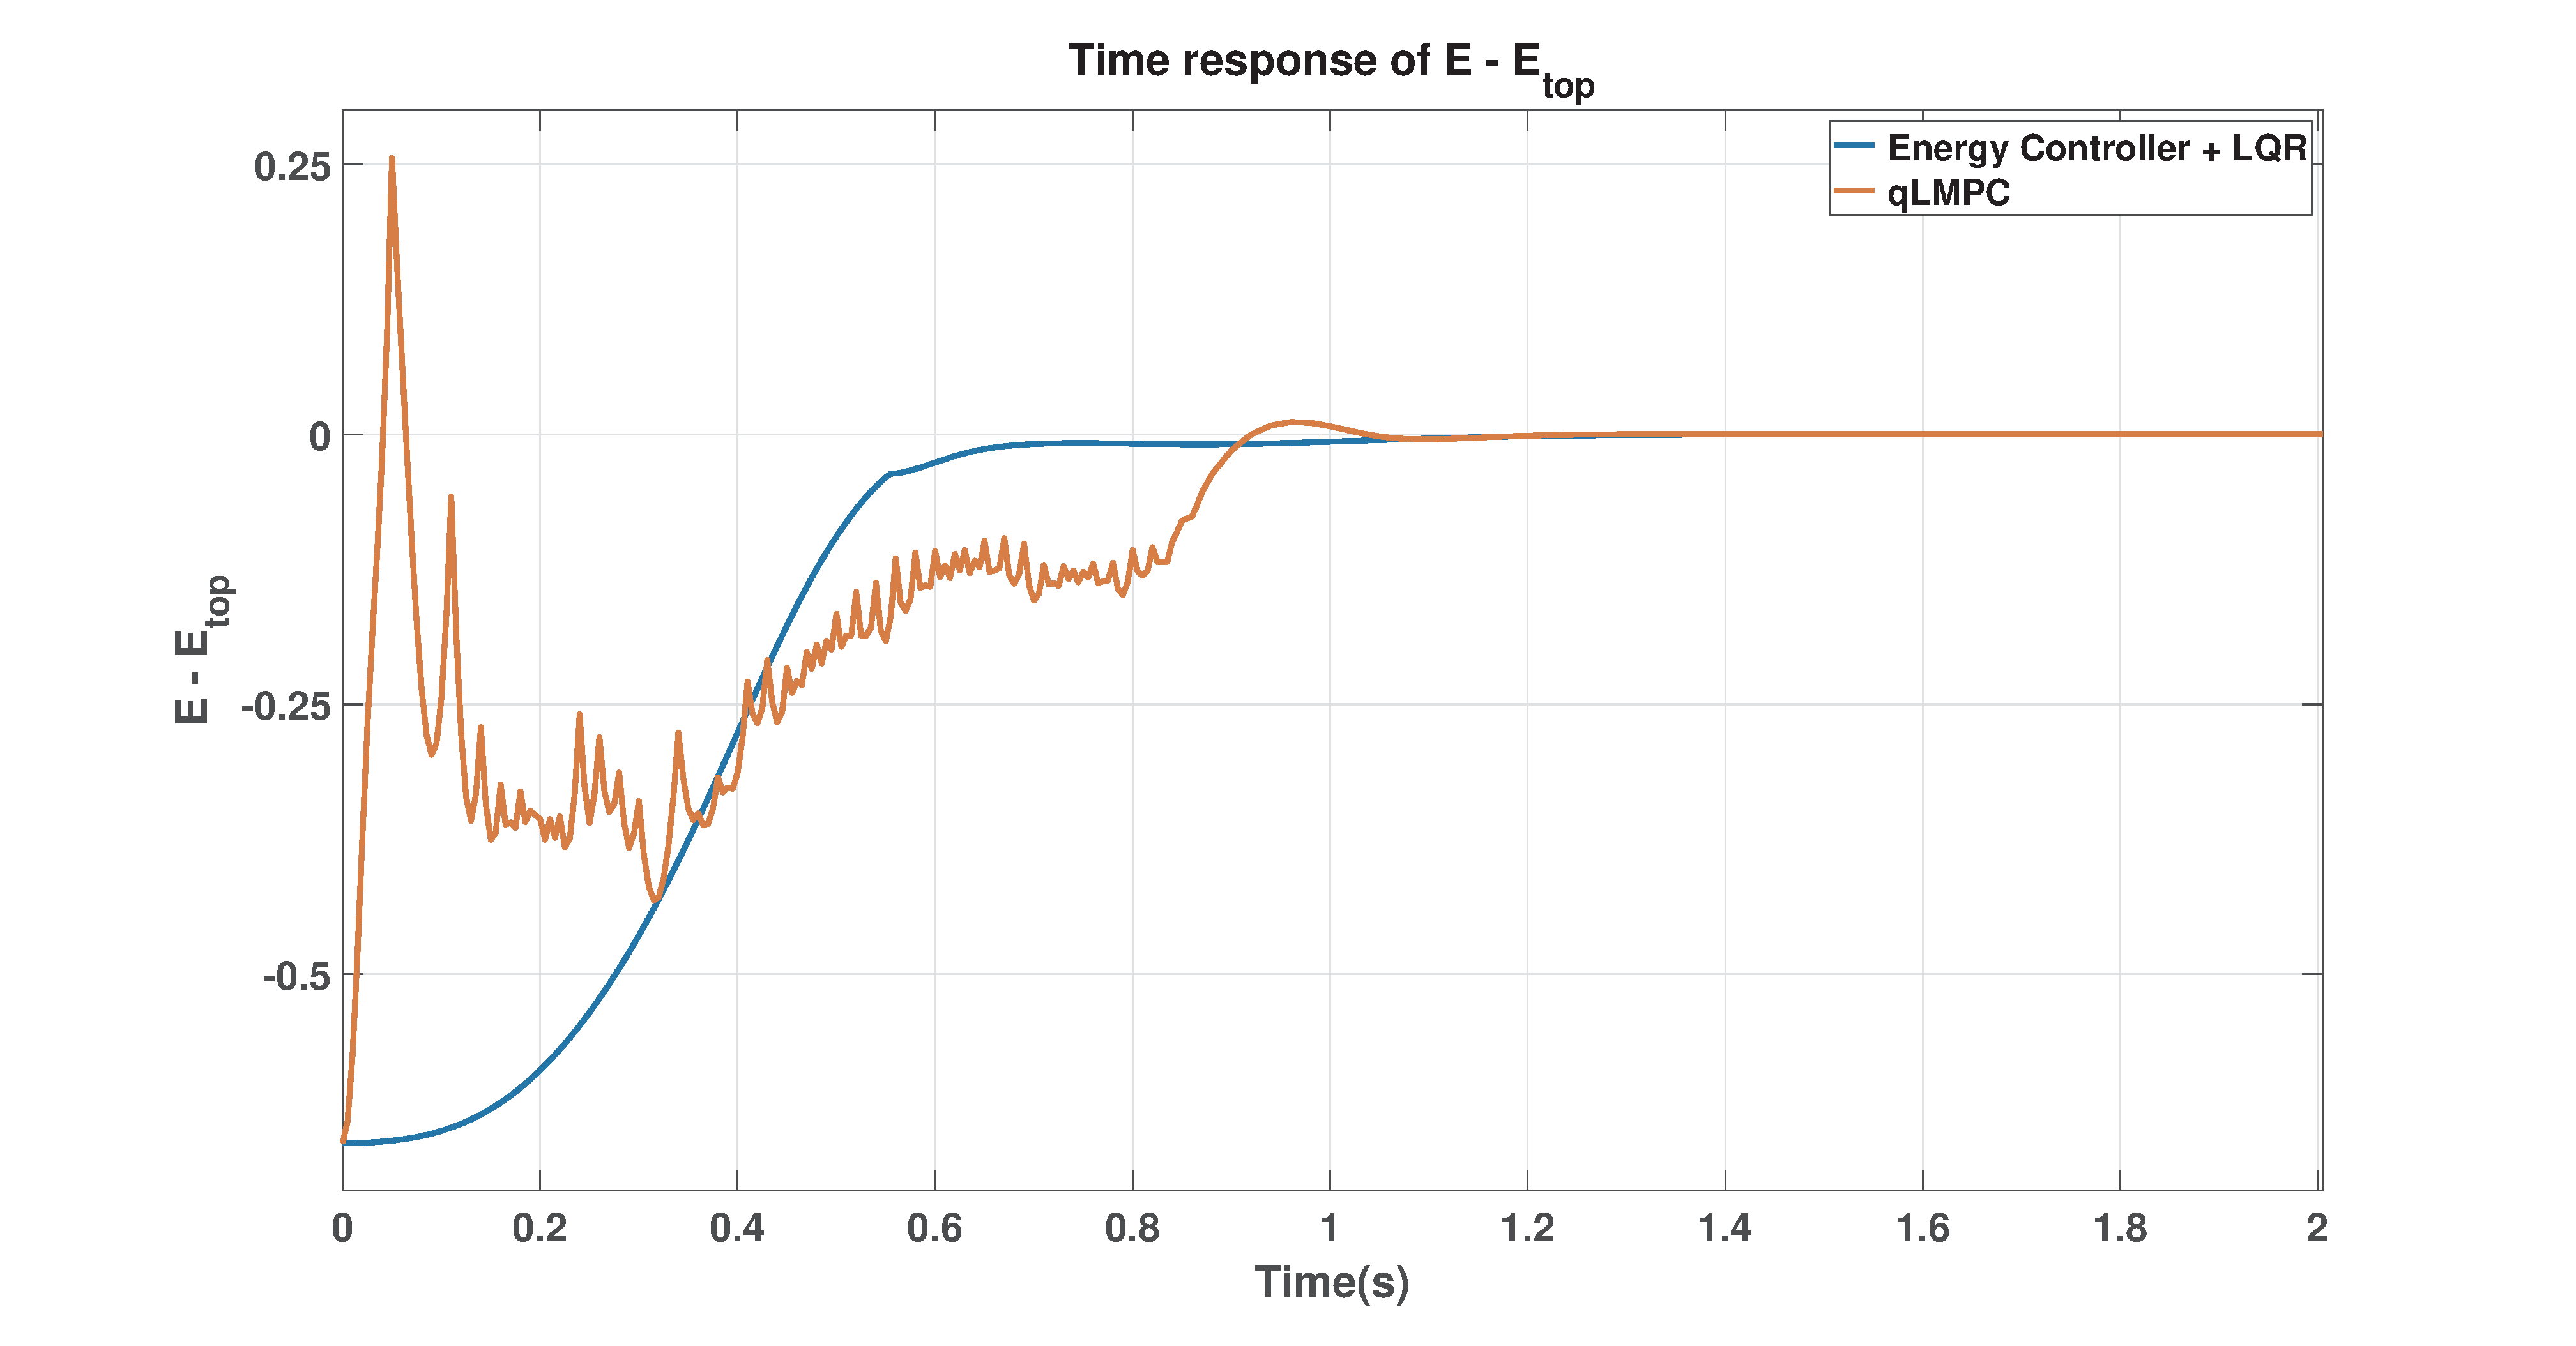
\includegraphics[width=0.84\textwidth]{figures/Etilda_comb}
    \caption{Time response of $\tilde{E}$.}
    \label{fig:Etilda}
\end{figure}
    % ~
    % \begin{subfigure}[t]{0.485\textwidth}
    % \centering
    % 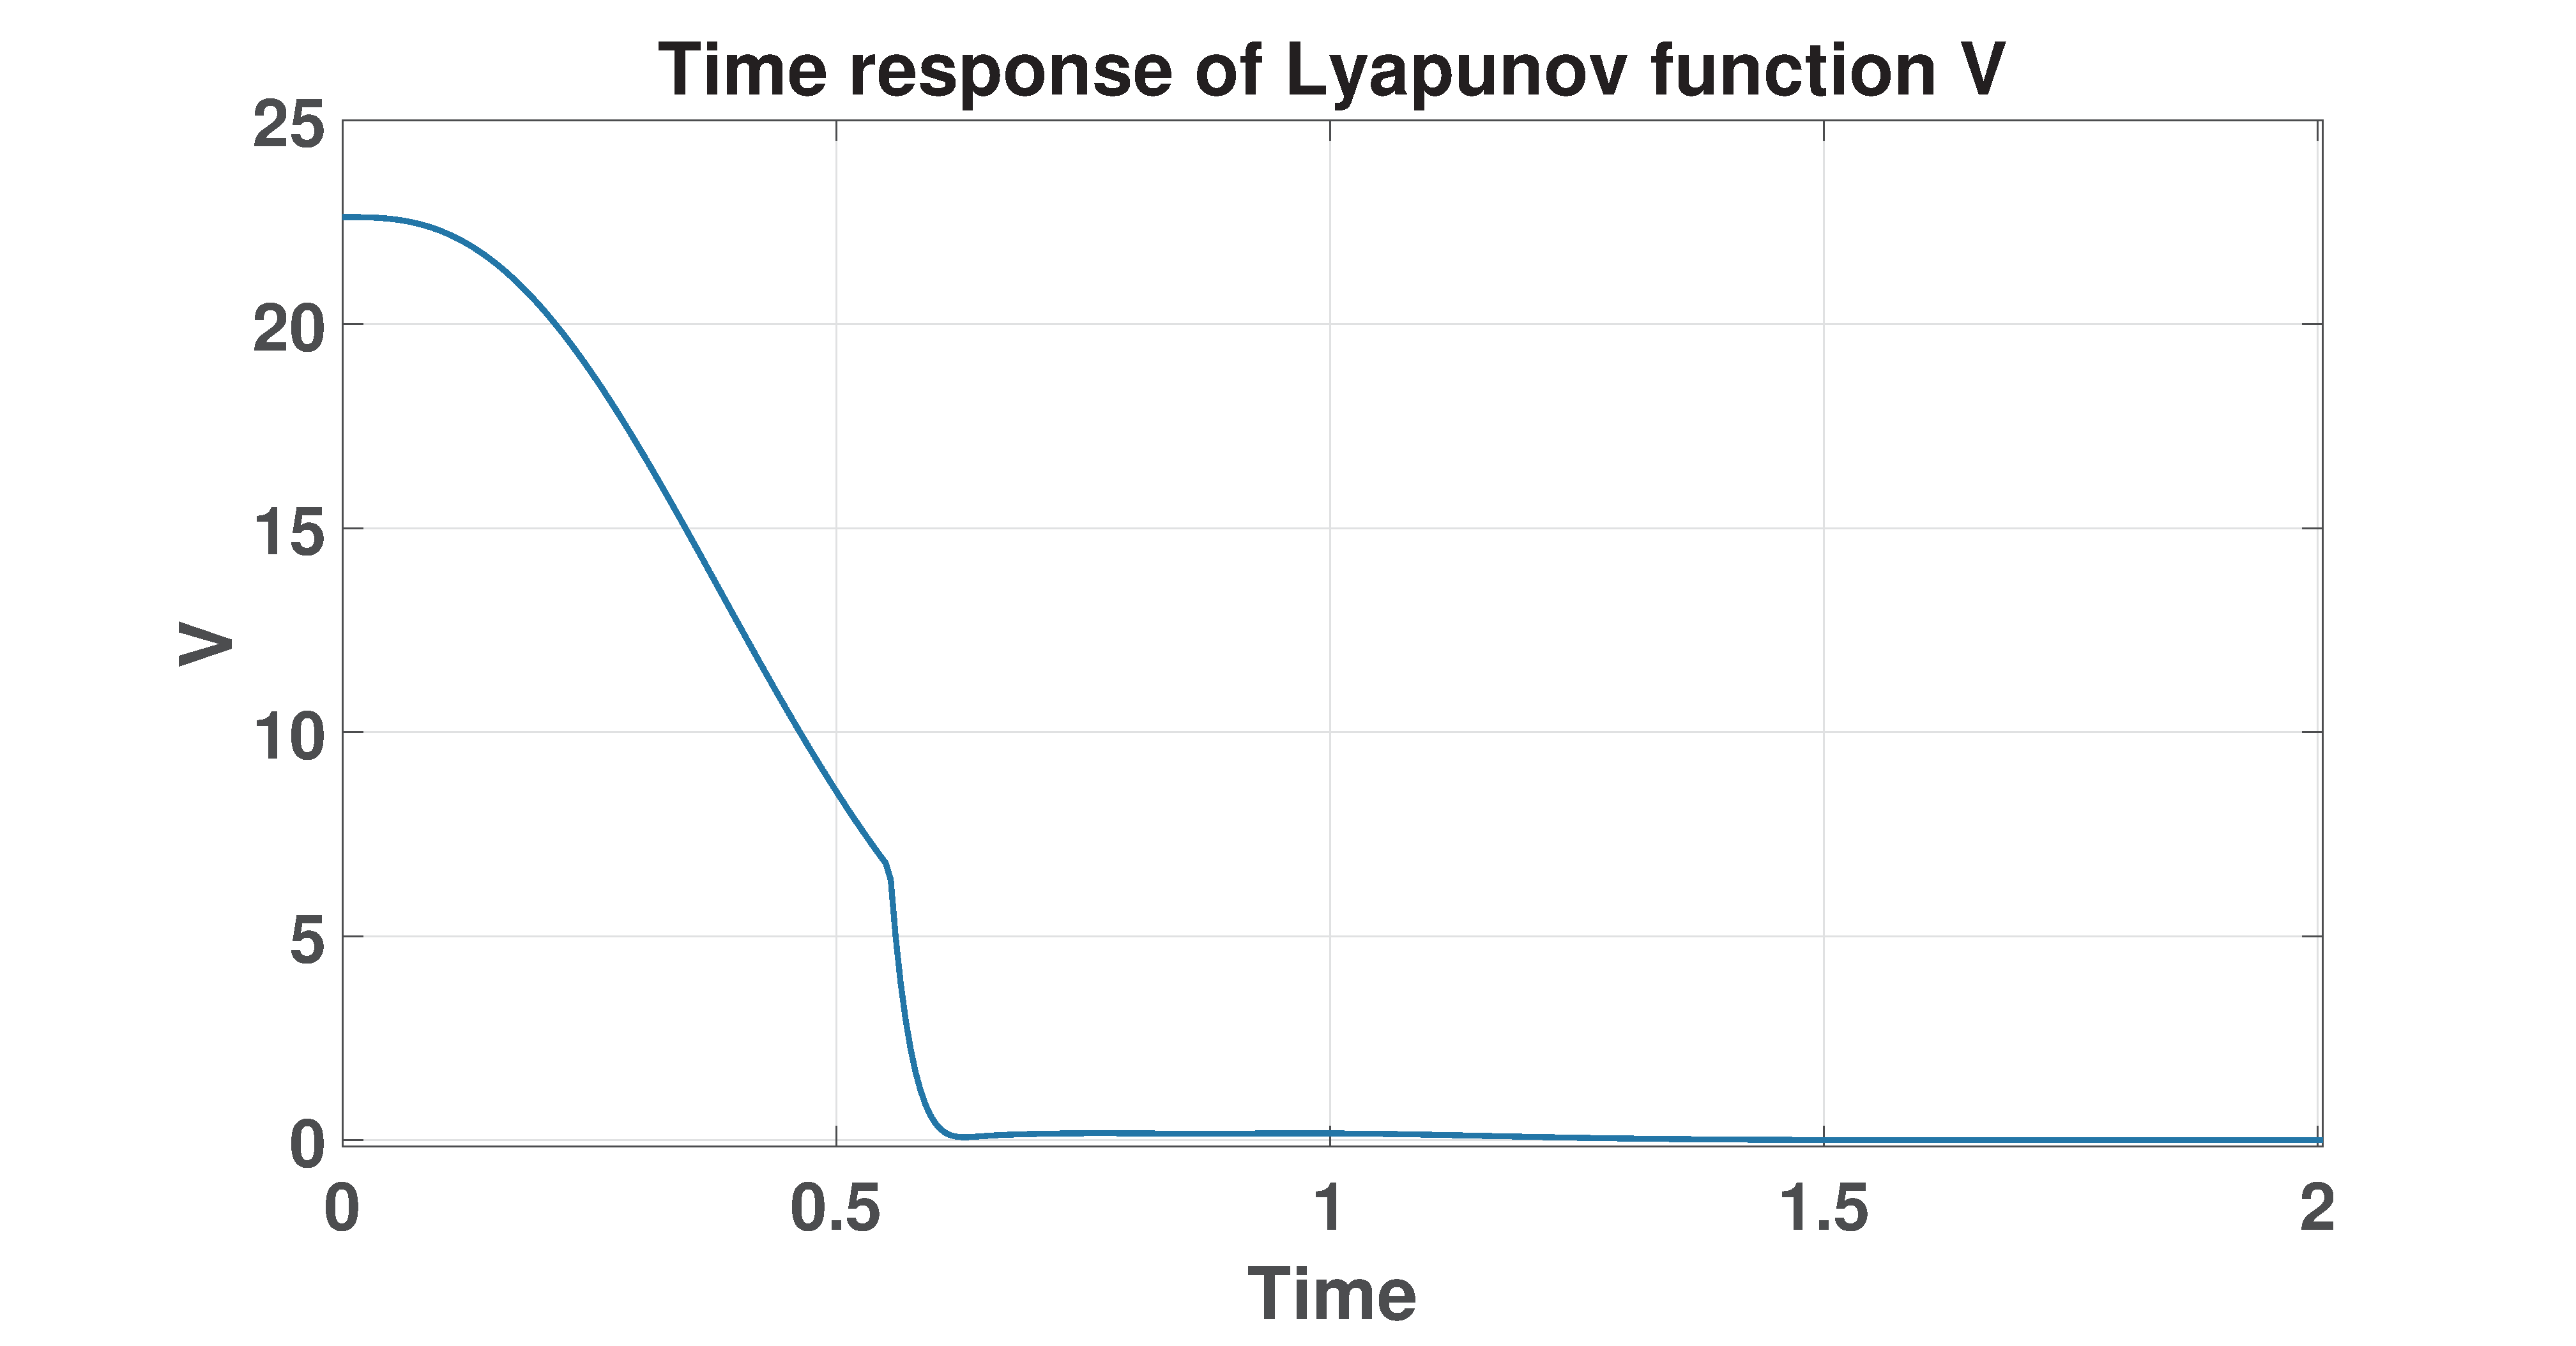
\includegraphics[width=\textwidth]{figures/Lyapunov}
    % \caption{Time response of Lyapunov function $V$.}
    % \label{fig:Lyapunov}
    % \end{subfigure}
    % \caption{Time responses}
% \end{figure}
% % 
% % There was also an attempt to isolate the dominant dynamics at the stable equillibrium and use them as observables at the unstable point, but this proved to be futile since things don't exactly work that easily. Talk about this.



}		% Simulation & Results
	{\include{contents/kapitel_5}} 	        %
    % 	
	\ifthenelse{\equal{\isenglish}{true}}%
	{\section{Conclusion and Future Scope}
\label{Chapter:Conc}
This thesis work focuses on the merits and demerits of implementing the Koopman operator theory for model-based control. The central idea of the Koopman operator framework is to lift the nonlinear dynamics of a system to a higher dimensional space where the evolution of dynamics becomes approximately linear. Such linear data-driven models were derived using known regression techniques like DMD~(Sec.~\ref{sec:DMD}) and EDMD~(Sec.~\ref{sec:EDMD}). Model-based controllers were then synthesized for such data-driven models, and the performance of the controllers was evaluated on a trajectory tracking problem. The data-driven models on a whole exhibit superior performance as compared to locally linearized models and moreover, linear control design methods could be readily applied to these models. It was observed that increasing the `complexity' of candidate functions, or in simple words, augmenting the state vector with nonlinear functions of the state further improved the performance of data-driven approximation models. For example, in the open-loop identification~(Sec~\ref{sec:Results_ident}), with the increasing complexity of the candidate functions, the SINDy regression algorithm could predict the state's evolution over a longer time period and for different operating conditions. It was also found that the prediction could be further improved when the data are sampled from various trajectories. The flexibility of data approximation methods allows for data from multiple trajectories and missing data points to be used. Furthermore, it was observed that the volume of data and its distribution across the state space has a significant effect on the computation of the Koopman operator.  \par
These vital observations obtained from open-loop identification were applied in recording the data for closed-loop identification since the Up-Up configuration is where the focus of this thesis work lies. The closed-loop performance of the data-driven controllers was compared to that of the locally linearized controllers. To this end, a first-principles model was derived~(Sec.~\ref{Sec:firstprinci}) and locally linearized by Jacobian linearization at the Up-Up position. Both a non-predictive controller such as the linear quadratic regulator and a predictive controller such as the model predictive controller were synthesized to compare the tracking performance in combination with the data-driven model. It was observed that non-predictive controllers do not perform as well as predictive controllers when the state is augmented with certain nonlinear functions of the state. It is hard to predict which functions might fail non-predictive controllers, and therefore, when working with data-driven models, it is recommended to work with predictive controllers. Moreover, the tracking performance of the predictive controller was far greater than the non-predictive controller~(Tab.~\ref{tab:RMSE_2}). And, with the recent advancement in computational capabilities, predictive control is much less cost-intensive than previously. Also, it must be noted that the computational complexity of a high-dimensional lifted system is rendered virtually independent of the dimension of the state by formulating the MPC problem using the so-called dense-form \cite{MPC_Korda}. Additionally, with a judicious choice of observables, it was observed that the data-driven models could capture nonlinearities that are otherwise not captured by locally linearized models. As a result, the tracking range of data-driven model-controllers could be significantly improved over the locally linearized model-controllers or even other data-driven models that are approximated with only measurements of state~(Fig.~\ref{fig: KPMC_comp}).\newpage
The robustness of tracking performance was tested for the data-driven model approximated with nonlinear functions of the state~(Fig.~\ref{fig: cont_traj}). It was observed that as the slope of trajectory became steeper, the performance of the data-driven model controller decreased. There could be two potential reasons for this. First, the set of observables or the nonlinear functions of the state may not be optimal in the sense of capturing the necessary nonlinearities, and there may exist some other combination of observables that perform better. The possibility of finding these `best' observables is left to the scope of future research. Second, the data-driven model's performance degradation may also be construed as a possible limitation of data-driven models. It must be noted that `extended' tracking range here means that the controller can track a trajectory beyond the range of trajectories used for training the data-driven model. Although the controller could successfully track an extended trajectory in a fairly good manner, as the slope of the trajectory increased, the controller could not perform as efficiently as desired. This could mean that the state-space in which the data-driven controllers can perform equally well or even better than the locally linearized first-principles model-controllers is limited to the range of training data. Nevertheless, the possibility of extending the range of a controller by simply augmenting the state with a wise choice of observables seems to be a promising area of research.\par
Moreover, the data-driven model was compared with a quasi-linear parameter varying model~(Fig.~\ref{fig: cont_traj_qLMPC}). Some interesting insights could be derived from this comparison. Firstly, although the qLMPC is a computationally expensive process compared with Koopman MPC, the computation time was well within the acceptable hardware limit. Second, the relative RMSE for a qLMPC was significantly lesser than that of the Koopman MPC. Moreover, Cisneros et al. \cite{qLMPC} were able to achieve up to $80^\circ$ as the maximum range of tracking. Therefore, it can be concluded that the first-principles model-based qLMPC performs much better than the Koopman MPC, which heavily depends on the choice of observables. However, one major assumption that is made here is the availability of the first-principles model. In the absence of a first-principles model, the Koopman model is a powerful and useful approximation of the underlying nonlinear dynamics. Thus, it can be said that the choice of model depends on the particular use case. \par
Finally, two different strategies to swing-up the pendulum from its stable equilibrium and balance it about its unstable equilibrium were evaluated. This comparison was made to investigate the possibility of swing-up using MPC controller and evaluate it against a proven swing-up law. The energy-based swing-up law proposed by Fantoni et al.~\cite{Fantoni} could achieve successful swing-up in just one swing as the swing-up law ensures the convergence of the pendulum trajectory to a homoclinic orbit around the unstable equilibrium. When the pendulum enters this homoclinic orbit, the controller is switched from an energy-based controller to a stabilizing controller such as the LQR to stabilize the pendulum about its unstable equilibrium. This is unlike the second strategy which employs the qLPV approach to linearize the plant at every time step and synthesize a corresponding model predictive controller. Although both the controllers achieve swing-up and stabilization in approximately the same time~(Sec.~\ref{sec: swingup}), it must be noted that the former approach employed two controllers, one for swing-up and one for stabilizing the pendulum, whereas the latter employs only a single controller to achieve both the swing-up and stabilization tasks.
\newpage
\subsubsection*{Future Scope}
In this thesis work, the observables, especially the RBFs, were chosen at random from a defined set. Although it became evident that a fortuitous set of observables significantly improved the performance of a tracking controller, the case for data-driven controllers can be strengthened if one could find a mathematical approach to exactly identify such observables. The SINDy algorithm is a good start in this research direction. One could also utilise any prior information of the particular dynamical system to discover such observables. However, one must think of a way to validate any such potential observables obtained based on physical insight or intuitive knowledge of the dynamics. Future work should also focus on proving or imposing closed-loop stability guarantees. An interesting direction for future work of this particular thesis work can be in the area of online-learning or active-learning, wherein a new Koopman model is learned online whenever novel dynamics are encountered. This is similar to a linear parameter varying model based on first-principles and has been explored for a Control Moment Gyroscope by Cisneros et al.~\cite{Cisneros.2020}.}		        % Conclusion
	{\section {Zusammenfassung und Ausblick}

Der vorliegenden Text gibt Studentinnen und Studenten, die am
Beginn der Niederschrift Ihrer Bachelor- oder Masterarbeit am
Arbeitsbereich Regelungstechnik sind eine Anleitung, welche Punkte
zu beachten sind, damit diese Arbeit gelingt.


Sicherlich wurden nicht alle Aspekte des Schreibens aufgeführt.
Für weitere Fragen steht Ihnen ja Ihr Betreuer ebenso zu
Verfügung. Nutzen Sie den Dialog nach der Korrektur einzelner
Abschnitte als geeignetes Mittel zur Verbesserung Ihres
schriftlichen Textes!
} 	        % Zusammenfassung
	
\printbibliography[title=\bibnamem]
\end{refsection} 

 %% Appendix ---------------------------------------------
\appendix

\end{document}

